\documentclass[british,a4paper,order=firstname]{mathscript}
\usepackage{mathoperators}

\title{\textbf{Applied statistics (spring term 2019)}}
\author{readers: Dr \person{Ksenia Shalonova} and Dr \person{Nikolai Bode}}
\date{written by \person{Henry Haustein}}

\begin{document}
\pagenumbering{roman}
\pagestyle{plain}

\maketitle

\hypertarget{tocpage}{}
\tableofcontents
\bookmark[dest=tocpage,level=1]{Table of contents}

\pagebreak
\pagenumbering{arabic}
\pagestyle{fancy}

\section{Estimating parameters}
\subsection{Confidence and tolerance intervals}

In statistical analysis we want to estimate a population from a \begriff{random sample}. This is called \begriff{interference} about the parameter. Random samples are used to provide information about parameters in an underlying \begriff{population distribution}. Rather than estimating the full shape of the underlying distribution, we usually focus on one or two parameters.

We want the error distribution to be centered on zero. Such an estimator is called \begriff{unbiased}. An biased estimator tends to have negative/positive errors, i.e. it usually underestimates/overestimates the parameter that is being estimated.

We also want \begriff{error distribution} to be tightly concentrated on zero, i.e. to have a small spread.

A good estimator should have a small bias and small standard error. These two criteria can be combined with into single value called the estimator's \begriff{mean squared error}. Most estimators that we will consider are unbiased, the spread of the error distribution is most important. 

\begin{definition}[Standard error]
    The \begriff{standard error} (SE) of an estimator $\hat{\theta}$ of a parameter $\theta$ is defined to be its standard deviation.
\end{definition}

\begin{example}
    Standard error of the mean:
    \begin{itemize}
        \item Bias ($\mu$ error) = 0, i.e. $E(\hat{\theta})=\theta$
        \item When population standard deviation is known: $\text{SE} = \frac{\sigma}{\sqrt{n}}$
        \item When population standard deviation is unknown: $\text{SE} = \frac{s}{\sqrt{n}}$
    \end{itemize}
\end{example}

Do not confuse SD (sample standard deviation) ($\to$ one sample) and SE (standard deviation of the sample mean $\bar{x}$) ($\to$ error from hypothetical samples)!

\begin{definition}[Confidence interval for $\mu$ with known $\sigma$]
    We can be $(1-\alpha)\cdot 100\%$ confident that the estimate for $\mu$ will be in the interval
    \begin{align}
        \bar{x} - z_{\nicefrac{\alpha}{2}}\frac{\sigma}{\sqrt{n}} < \mu < \bar{x} + z_{\nicefrac{\alpha}{2}}\frac{\sigma}{\sqrt{n}} \notag
    \end{align}
    
    Common exact values of $z_{\nicefrac{\alpha}{2}}$ with critical values from normal distribution:
    \begin{center}
        \begin{tabular}{c|c}
            \textbf{confidence} & \textbf{value of $z_{\nicefrac{\alpha}{2}}$} \\
            \hline
            90\% & 1.645 \\
            95\% & 1.96 \\
            99\% & 2.575 \\
        \end{tabular}
    \end{center}
\end{definition}

\begin{definition}[Confidence interval for $\mu$ when $\sigma$ is unknown]
    If we simply replace $\sigma$ by its sample variance the confidence level will be lower than 95\%. When the sample size is large, the confidence level is close to 95\% but the confidence level can be much lower if the sample size is small. 
    
    Critical value comes from the \person{Students} t distribution. The value of $t_{\nicefrac{\alpha}{2}}$ depends on the sample size through the use of degrees of freedom. The confidence interval is
    \begin{align}
        \bar{x} - t_{\nicefrac{\alpha}{2}}\frac{s}{\sqrt{n}} < \mu < \bar{x} + t_{\nicefrac{\alpha}{2}}\frac{s}{\sqrt{n}} \notag
    \end{align}
\end{definition}

Consider estimation of a population mean, $\mu$, from a random sample of size $n$. A confidence interval will be of the form $\bar{x}\pm t_{\nicefrac{\alpha}{2}}\frac{s}{\sqrt{n}}$. If we want our estimate to be within $k$ of $\mu$, then we need $n$ to be large enough so that $t_{\nicefrac{\alpha}{2}}\frac{s}{\sqrt{n}} < k$. For 95\% confidence interval if $n$ is reasonably large the t-value in the inequality will be approximately 1.96: $1.96\frac{s}{\sqrt{n}}<k$ that can be re-written as $n>\left(\frac{1.96s}{k}\right)^2$. In practice, it is best to increase $n$ a little over this value in case the sample deviation was wrongly guessed.

\begin{example}
    If we expect that a particular type of measurement will have a standard deviation of about 8, and we want to estimate its mean, $\mu$, to within 2 of its correct value with probability 0.95, the sample size should be:
    \begin{align}
        n>\left(\frac{1.96\cdot 8}{2}\right)^2 = 61.5\notag
    \end{align}
    This suggests a sample size of at least 62. The more accurate trial-and-error method using a t-value would give a sample size of 64.
\end{example}

The sample proportion of successes is denoted by $\hat{p}$ and is an estimate of $p$. The estimation error is $\hat{p}-p$.
\begin{align}
    \hat{p} = \frac{\text{number of successes in sample}}{\text{sample size}} \notag
\end{align}
A 95\% confidence interval is $\hat{p} \pm 2\cdot\sqrt{\frac{p(1-p)}{n}}$

\begin{example}
    In a random sample of $n=36$ values, there were $x=17$ successes. We estimate the population proportion $\hat{p}$ with $\hat{p}=\frac{17}{36}=0.472$. A 95\% confidence interval for $\hat{p}$ is $0.472\pm 0.166$. We are therefor 95\% confident that the population of successes is between 30.6\% and 63.8\%. A sample size of $n=36$ is clearly too small to give a very accurate estimate.
    
    If the sample  size $n$ is small or $\hat{p}$ is close to either 0 or 1, this normal approximation is inaccurate and the confidence level for the interval can be considerably less than 95\%. Classical theory recommends to use the confidence interval for $\hat{p}$ only when $n>30$, $n\hat{p}>5$ and $n(1-\hat{p})>5$.
\end{example}

\begin{*anmerkung}[z-value or t-value?]
    \begin{itemize}
        \item If you know the variance of the population, then you should use the z-value from normal distribution.
        \item If you don't know the variance of the population or the population is non-normal, then you should formally always use the t-value.
        \item For most non-normal population distributions, the distribution of the sample mean becomes close to normal when the sample size increases (\begriff{Central Limit Theorem})
        \item Even for relatively small samples, the distributions are virtually the same. Therefore, it is common to approximate the t-distribution using normal distribution for sufficiently large samples (e.g. $n>30$).
    \end{itemize}
\end{*anmerkung}

\begin{definition}[Tolerance interval]
    A $(1-\alpha)\cdot 100\%$ \begriff{tolerance interval} for $\gamma\cdot 100\%$ of the measurements in a normal population is given by $\bar{x}\pm Ks$ where $K$ is a tolerance factor. \begriff{Tolerance limits} are the endpoints of the tolerance interval.
\end{definition}

Do not mix up with confidence intervals! We focus on $\gamma$ (a certain percentage of measurements) rather than on a population parameter.

If we knew $\mu$ and $\sigma$ then the tolerance factor $K$ is 1. Otherwise the tolerance factor depends on the level of confidence, $\gamma$ and the sample size $n$. 

\begin{example}
    A corporation manufactures field rifles. To monitor the process, an inspector randomly selected 50 firing pins from the production line. The sample mean $\bar{x}$ for all observations is 0.9958 inch and standard deviation $s$ is 0.0333. Assume that the distribution of pin lengths is normal. Find a 95\% tolerance interval for 90\% of the firing pin lengths.
    
    Given $n=50$, $\gamma=0.9$ and $\alpha=0.05$, work out $K$ (you can either use a special table or MATLAB function). $K=1.996$. The 95\% tolerance interval is (0.9293, 1.0623). Approximately 95 of 100 similarly constructed tolerance intervals will contain 90\% of the firing pin lengths in the population.
\end{example}
\subsection{Maximum Likelihood Estimate}

\begin{definition}[likelihood function]
    If random variables have joint probability $p(x_1,...,x_n\vert \theta)$ then the function $L(\theta\vert x_1,...,x_n)=p(x_1,...,x_n\vert\theta)$ is called the \begriff{likelihood function} of $\theta$.
\end{definition}

The likelihood function tells the probability of getting the data that were observed if the parameter value was really $\theta$.

\begin{definition}[maximum likelihood estimate]
    The \begriff{maximum likelihood estimate} of a parameter $\theta$ is the value that maximizes the likelihood function $L(\theta\vert x_1,...,x_n) = p(x_1,...,x_n\vert\theta)$.
\end{definition}

In practice they maximize the logarithm of the likelihood function and solve the following equation:
\begin{align}
    \frac{\mathrm{d}\log L(\theta\vert x_1,...,x_n)}{\mathrm{d}\theta}\notag
\end{align}

The following formula can find an approximate numerical value for the standard error of almost any maximum likelihood estimator:
\begin{align}
    \SE(\hat{\theta}) \approx\sqrt{-\frac{1}{l''(\hat{\theta})}}\notag
\end{align}
For the 95\% confidence interval we can write:
\begin{align}
    \hat{\theta} - 1.96\cdot\SE(\hat{\theta}) < \theta < \hat{\theta} + 1.96\cdot\SE(\hat{\theta}) \notag
\end{align}
For the 90\% confidence interval we can write:
\begin{align}
    \hat{\theta} - 1.645\cdot\SE(\hat{\theta}) < \theta < \hat{\theta} + 1.645\cdot\SE(\hat{\theta}) \notag
\end{align}

\begin{example}
    The probability density function (PDF) of exponential distribution is
    \begin{align}
        \PDF = \begin{cases}
            \lambda e^{-\lambda x} & x\ge 0 \\ 0 & \text{otherwise}
        \end{cases}\notag
    \end{align}
    We want to estimate the parameter $\lambda$. 
    \begin{center}
       \begin{tabular}{p{4cm}|p{7cm}}
            Likelihood function & $L(\lambda\vert x_1,...,x_n) = \lambda^n e^{-\lambda\sum x_i}$ \\
            \hline
            log-likelihood function & $l(\lambda\vert x_1,...,x_n) = n\log(\lambda)-\lambda\sum x_i$ \\
            \hline
            MLE & $l'(\lambda\vert x_1,...,x_n) = \frac{n}{\lambda} - \sum x_i \overset{!}{=} 0\Rightarrow \hat{\lambda} = \frac{1}{\bar{x}}$ \\
            \hline
            Standard error & $\SE(\hat{\lambda}) = \sqrt{-\frac{1}{l''(\hat{\lambda})}} = \frac{\hat{\lambda}}{\sqrt{n}} = \frac{1}{\sqrt{n}\bar{x}}$ where $l''(\lambda) = -\frac{n}{\lambda^2}$ \\
            \hline
            95\% confidence interval & $\frac{1}{\bar{x}}\pm 1.96\cdot\frac{1}{\sqrt{n}\bar{x}}$
       \end{tabular}
    \end{center}
    
    Lets assume that the mean time between failures of 199 air-conditioners is $\bar{x} = 90.92$ hours. The MLE for the estimated failure rate $\lambda$ is $\frac{1}{\bar{x}} = 0.0110$ failure per hour. \\
    $\Rightarrow$ 95\% confidence interval for the failure rate:
    \begin{align}
        \frac{1}{\bar{x}} \pm 1.96\cdot\frac{1}{\sqrt{n}\bar{x}} \Rightarrow \lambda\in [0.00974,0.01253]\notag
    \end{align}
\end{example}    
    
Given a sample, we can estimate two unknown parameters in a probability distribution, for example, estimate parameters $\mu$ and $\sigma$ in a normal distribution.
    
\begin{definition}[likelihood function for two parameters]
    If random variables have joint probability $p(x_1,...,x_n\vert \theta,\phi)$ then the function $L(\theta,\phi\vert x_1,...,x_n)=p(x_1,...,x_n\vert\theta,\phi)$ is called the \begriff{likelihood function} of $\theta$ and $\phi$.
\end{definition}

The likelihood function is maximised at a turning point of the likelihood function and could therefore be found by setting the partial derivatives of $L(\theta,\phi)$ with respect to $\theta$ and $\phi$ to zero.

There are two important properties of the maximum likelihood estimator $\hat{\theta}$ of a parameter $\theta$ based on a random sample of size $n$ from a distribution with a probability function $p(x_1,...,x_n\vert\theta)$:
\begin{itemize}
    \item Asymptotically unbiased: $E(\hat{\theta})\to\theta$ when $n\to\infty$
    \item Asymptotically has a normal distribution: $\hat{\theta}\to$ normal distribution when $n\to\infty$ that can be used to generate confidence intervals.
    \item Maximum likelihood estimators have low mean squared error if the sample size is large enough. MLE can be heavily biased for small samples!
\end{itemize}

\subsection{Continuous distributions}

The \begriff{lognormal distribution} is used in situations where values are positively skewed, for example, for financial analysis of stock prices. Note that the uncertain variable can increase without limits but cannot take negative values.
\begin{center}
    \begin{tikzpicture}
            \begin{axis}[
		    xmin=0, xmax=2, xlabel=$x$,
		    ymin=0, ymax=1, ylabel=$y$,
		    samples=400,
		    axis y line=middle,
		    axis x line=middle,
		    restrict y to domain=0:1,
		    ]
		    \addplot+[mark=none] {1/(x*sqrt(2*pi))*exp(-0.5*(ln(x))^2)};
		    \addlegendentry{$\mu=0$, $\sigma=1$}
		    \end{axis}
        \end{tikzpicture}
\end{center}

In the \begriff{beta distribution} the uncertain variable is a random value between 0 and  positive value. The distribution is frequently used for estimating the proportions and probabilities (i.e. values between 0 and 1). The shape of the distribution is specified by two positive parameters.

The \begriff{\person{Students} t distribution} is the most widely used distribution in confidence intervals and hypothesis testing. The distribution can be used to estimate the mean of a normally distributed population when the sample size is small. The t distribution comes to approximate the normal distribution as the degrees of freedom (or sample size) increases.
\begin{center}
    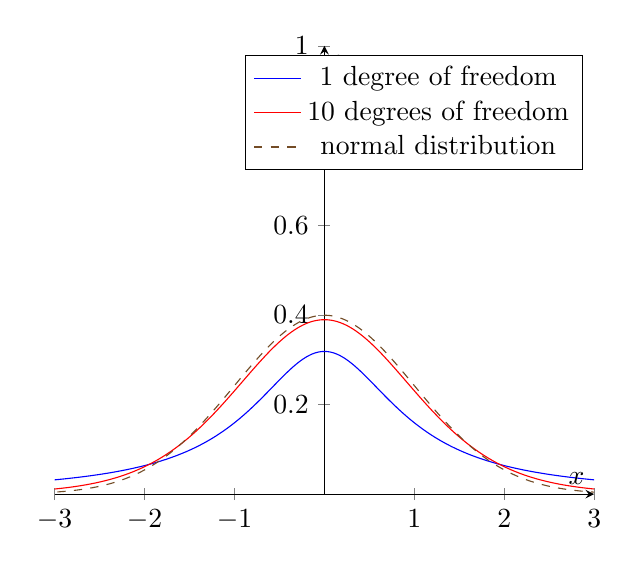
\begin{tikzpicture}
            \begin{axis}[
		    xmin=-3, xmax=3, xlabel=$x$,
		    ymin=0, ymax=1, ylabel=$y$,
		    samples=400,
		    axis y line=middle,
		    axis x line=middle,
		    ]
		    \addplot+[mark=none] {(1)/(pi*(x^2+1))};
		    \addlegendentry{1 degree of freedom}
		    \addplot+[mark=none] {0.389108/((1+x^2/10)^5.5)};
		    \addlegendentry{10 degrees of freedom}
		    \addplot+[dashed,mark=none] {1/(sqrt(2*pi))*exp(-0.5*x^2)};
		    \addlegendentry{normal distribution}
		    \end{axis}
        \end{tikzpicture}
\end{center}

The \begriff{chi-square distribution} is usually used for estimating the variance in a normal distribution.
\begin{center}
	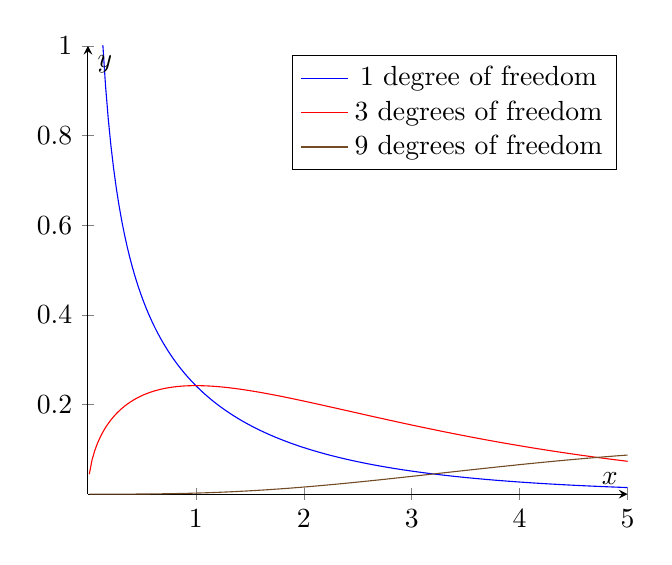
\begin{tikzpicture}
	\begin{axis}[
	xmin=0, xmax=5, xlabel=$x$,
	ymin=0, ymax=1, ylabel=$y$,
	samples=400,
	axis y line=middle,
	axis x line=middle,
	]
	\addplot+[mark=none] {exp(-x/2)/(sqrt(2*pi) * sqrt(x))};
	\addlegendentry{1 degree of freedom}
	\addplot+[mark=none] {exp(-x/2) * sqrt(x)/sqrt(2*pi)};
	\addlegendentry{3 degrees of freedom}
	\addplot+[mark=none] {exp(-x/2) * x^(7/2)/(105 * sqrt(2*pi))};
	\addlegendentry{9 degrees of freedom}
	\end{axis}
	\end{tikzpicture}
\end{center}

In a homogeneous \person{Poisson} process with a rate $\lambda$ events per unit time, the time until the first event happens has a distribution called an \begriff{exponential distribution}. All exponential distributions have their highest probability density at $x=0$ and steadily decrease as $x$ increases.
\begin{center}
    \begin{tikzpicture}
            \begin{axis}[
		    xmin=0, xmax=2, xlabel=$x$,
		    ymin=0, ymax=1, ylabel=$y$,
		    samples=400,
		    axis y line=middle,
		    axis x line=middle,
		    restrict y to domain=0:1,
		    ]
		    \addplot+[mark=none] {exp(-x)};
		    \addlegendentry{$\mu=1$}
		    \end{axis}
        \end{tikzpicture}
\end{center}

The \begriff{\person{Weibull} distribution} can be used as a model for items that either deteriorate or improve over time. It's basic version has two parameters: shape and scale.
\begin{center}
    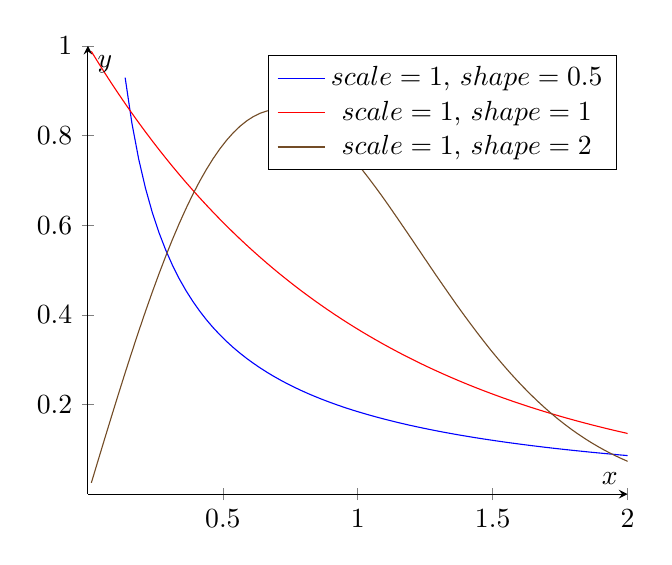
\begin{tikzpicture}
            \begin{axis}[
		    xmin=0, xmax=2, xlabel=$x$,
		    ymin=0, ymax=1, ylabel=$y$,
		    samples=400,
		    axis y line=middle,
		    axis x line=middle,
		    restrict y to domain=0:1,
		    ]
		    \addplot+[mark=none] {0.5*x^(-0.5)*exp(-x^0.5)};
		    \addlegendentry{$scale=1$, $shape=0.5$}
		    \addplot+[mark=none] {1/exp(x)};
		    \addlegendentry{$scale=1$, $shape=1$}
		    \addplot+[mark=none] {2*x^(1)*exp(-x^2)};
		    \addlegendentry{$scale=1$, $shape=2$}
		    \end{axis}
    \end{tikzpicture}
\end{center}
\begin{itemize}
    \item $shape>1$: the hazard function is increasing so the item becomes less reliable as it gets older.
    \item $shape<1$: the hazard function is decreasing so the item becomes more reliable as it gets older.
    \item $shape=1$: the hazard function is constant so the lifetime distribution becomes exponential.
\end{itemize}

The \begriff{survival function} (probability of surviving until a particular time) is $R(t) = 1-F(t)$. The \begriff{hazard rate function} (failure rate) is worked out by the formula:
\begin{align}
    h(t) &= \frac{f(t)}{1-F(t)} \notag \\
    &= \frac{f(t)}{R(t)} \notag
\end{align}
where $f(t)$ and $F(t)$ are PDF and CDF of the distribution.

The hazard function describes how an item ages where $t$ affects its risk of failure. This constant hazard function in the exponential distribution corresponds to the \person{Poisson} process without memory, i.e. the chance of failing does not depend on what happened before and how long the item has already survived.
\pagebreak
\section{Hypothesis testing}
There are two types of questions in statistical interference:
\begin{itemize}
    \item \textbf{Parameter estimation:} What parameter values would be consistent with the sample data?
    \item \textbf{Hypothesis testing:} Are the sample data consistent with some statement about the parameters?
\end{itemize}

The \begriff{Null Hypothesis} $H_0$ often specifies a single value for the unknown parameter such as "$\alpha = \dots$". It is a default value that can be accepted as holding if there is no evidence against it. A researcher often collects data with the express hope of disapproving the null hypothesis.

If the null hypothesis is not true, we say that the \begriff{alternative hypothesis} $H_A$ holds. If the data are not consistent with the null hypothesis, then we can conclude that the alternative hypothesis must be true. Either the null hypothesis or the alternative hypothesis must be true.

\begin{example}
    The data show the number of operating hours between successive failures of air-conditioning equipment in ten aircrafts. The sample of 199 values is a \begriff{test statistic}. We can test the manufacturer's claim that the rate of failures is no more than one per 110 hours of use.
    \begin{align}
        H_0: \lambda &\le \frac{1}{100}\text{ (claim of a manufacturer)} \notag \\
        H_A: \lambda &> \frac{1}{100} \notag
    \end{align}
    This can be simplified: \\
    \begin{align}
        H_0: \lambda &= \frac{1}{100}\text{ (claim of a manufacturer)} \notag \\
        H_A: \lambda &> \frac{1}{100} \notag
    \end{align}
\end{example}

\subsection{The P-value (Probability value)}

In an industrial process some measurement is normally distributed with standard deviation $\sigma = 10$. Its mean should be $\mu = 520$, but can differ a little bit. Samples of $n=10$ measurements are regularly collected as part of quality control. If a sample had $\bar{x}=529$, does the process need to be adjusted?

\begin{center}
    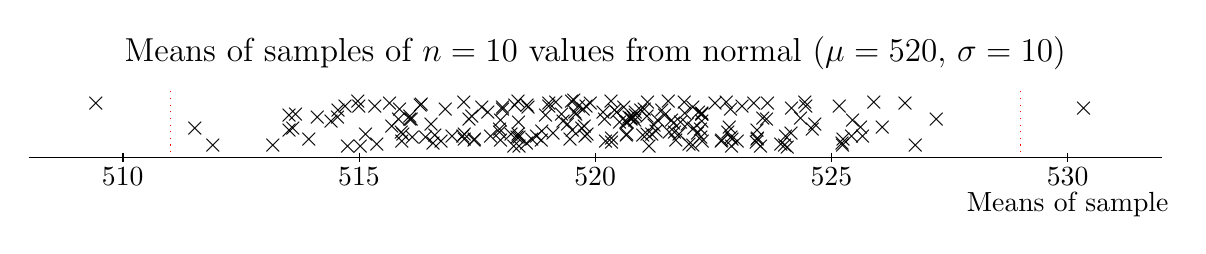
\begin{tikzpicture}[scale=0.6]
		\node at (525.23,0.09) (1) {$\times$};
		\node at (521.10,0.67) (2) {$\times$};
		\node at (519.55,1.00) (3) {$\times$};
		\node at (518.37,0.28) (4) {$\times$};
		\node at (522.27,0.13) (5) {$\times$};
		\node at (522.26,0.55) (6) {$\times$};
		\node at (509.43,0.93) (7) {$\times$};
		\node at (518.28,0.02) (8) {$\times$};
		\node at (522.19,0.74) (9) {$\times$};
		\node at (520.17,0.75) (10) {$\times$};
		\node at (520.22,0.13) (11) {$\times$};
		\node at (519.52,0.37) (12) {$\times$};
		\node at (519.65,0.88) (13) {$\times$};
		\node at (519.50,0.98) (14) {$\times$};
		\node at (515.93,0.28) (15) {$\times$};
		\node at (517.45,0.18) (16) {$\times$};
		\node at (524.65,0.49) (17) {$\times$};
		\node at (520.52,0.54) (18) {$\times$};
		\node at (517.60,0.85) (19) {$\times$};
		\node at (524.15,0.30) (20) {$\times$};
		\node at (521.90,0.73) (21) {$\times$};
		\node at (520.34,0.99) (22) {$\times$};
		\node at (521.04,0.82) (23) {$\times$};
		\node at (525.24,0.06) (24) {$\times$};
		\node at (513.66,0.70) (25) {$\times$};
		\node at (518.39,0.02) (26) {$\times$};
		\node at (520.46,0.76) (27) {$\times$};
		\node at (515.86,0.82) (28) {$\times$};
		\node at (515.90,0.32) (29) {$\times$};
		\node at (519.11,0.31) (30) {$\times$};
		\node at (518.38,0.54) (31) {$\times$};
		\node at (514.55,0.65) (32) {$\times$};
		\node at (524.35,0.63) (33) {$\times$};
		\node at (520.66,0.26) (34) {$\times$};
		\node at (522.26,0.72) (35) {$\times$};
		\node at (519.90,0.94) (36) {$\times$};
		\node at (521.55,0.99) (37) {$\times$};
		\node at (524.03,0.25) (38) {$\times$};
		\node at (521.99,0.07) (39) {$\times$};
		\node at (513.94,0.18) (40) {$\times$};
		\node at (521.20,0.28) (41) {$\times$};
		\node at (524.44,0.97) (42) {$\times$};
		\node at (518.39,0.22) (43) {$\times$};
		\node at (518.56,0.89) (44) {$\times$};
		\node at (518.95,0.69) (45) {$\times$};
		\node at (522.26,0.71) (46) {$\times$};
		\node at (530.34,0.84) (47) {$\times$};
		\node at (516.74,0.13) (48) {$\times$};
		\node at (520.68,0.54) (49) {$\times$};
		\node at (521.57,0.33) (50) {$\times$};
		\node at (523.36,0.93) (51) {$\times$};
		\node at (518.58,0.86) (52) {$\times$};
		\node at (519.83,0.28) (53) {$\times$};
		\node at (519.77,0.45) (54) {$\times$};
		\node at (517.39,0.67) (55) {$\times$};
		\node at (521.89,0.97) (56) {$\times$};
		\node at (514.41,0.56) (57) {$\times$};
		\node at (525.90,0.97) (58) {$\times$};
		\node at (521.62,0.59) (59) {$\times$};
		\node at (523.65,0.93) (60) {$\times$};
		\node at (521.68,0.33) (61) {$\times$};
		\node at (522.09,0.41) (62) {$\times$};
		\node at (519.02,0.88) (63) {$\times$};
		\node at (521.95,0.50) (64) {$\times$};
		\node at (514.71,0.88) (65) {$\times$};
		\node at (521.41,0.79) (66) {$\times$};
		\node at (523.43,0.37) (67) {$\times$};
		\node at (521.81,0.53) (68) {$\times$};
		\node at (521.29,0.34) (69) {$\times$};
		\node at (523.50,0.03) (70) {$\times$};
		\node at (520.85,0.76) (71) {$\times$};
		\node at (522.87,0.82) (72) {$\times$};
		\node at (522.07,0.86) (73) {$\times$};
		\node at (521.25,0.48) (74) {$\times$};
		\node at (521.78,0.28) (75) {$\times$};
		\node at (519.72,0.42) (76) {$\times$};
		\node at (522.24,0.22) (77) {$\times$};
		\node at (515.84,0.61) (78) {$\times$};
		\node at (522.90,0.17) (79) {$\times$};
		\node at (515.03,0.03) (80) {$\times$};
		\node at (520.84,0.59) (81) {$\times$};
		\node at (523.55,0.63) (82) {$\times$};
		\node at (517.79,0.24) (83) {$\times$};
		\node at (520.65,0.54) (84) {$\times$};
		\node at (518.35,0.22) (85) {$\times$};
		\node at (522.88,0.22) (86) {$\times$};
		\node at (514.12,0.65) (87) {$\times$};
		\node at (517.22,0.96) (88) {$\times$};
		\node at (515.34,0.88) (89) {$\times$};
		\node at (511.53,0.42) (90) {$\times$};
		\node at (518.22,0.28) (91) {$\times$};
		\node at (519.59,0.71) (92) {$\times$};
		\node at (522.17,0.31) (93) {$\times$};
		\node at (524.46,0.87) (94) {$\times$};
		\node at (520.20,0.60) (95) {$\times$};
		\node at (518.04,0.86) (96) {$\times$};
		\node at (525.25,0.18) (97) {$\times$};
		\node at (518.30,0.90) (98) {$\times$};
		\node at (517.44,0.16) (99) {$\times$};
		\node at (518.04,0.82) (100) {$\times$};
		\node at (516.83,0.81) (101) {$\times$};
		\node at (522.26,0.70) (102) {$\times$};
		\node at (520.81,0.65) (103) {$\times$};
		\node at (520.61,0.85) (104) {$\times$};
		\node at (522.54,0.95) (105) {$\times$};
		\node at (522.07,0.05) (106) {$\times$};
		\node at (515.14,0.28) (107) {$\times$};
		\node at (521.14,0.04) (108) {$\times$};
		\node at (516.08,0.61) (109) {$\times$};
		\node at (516.57,0.10) (110) {$\times$};
		\node at (525.45,0.59) (111) {$\times$};
		\node at (521.47,0.68) (112) {$\times$};
		\node at (516.13,0.21) (113) {$\times$};
		\node at (518.00,0.16) (114) {$\times$};
		\node at (524.16,0.84) (115) {$\times$};
		\node at (518.87,0.34) (116) {$\times$};
		\node at (515.00,0.88) (117) {$\times$};
		\node at (519.75,0.81) (118) {$\times$};
		\node at (520.41,0.80) (119) {$\times$};
		\node at (522.23,0.39) (120) {$\times$};
		\node at (523.63,0.61) (121) {$\times$};
		\node at (526.56,0.94) (122) {$\times$};
		\node at (521.32,0.58) (123) {$\times$};
		\node at (526.08,0.43) (124) {$\times$};
		\node at (513.60,0.42) (125) {$\times$};
		\node at (520.35,0.19) (126) {$\times$};
		\node at (517.73,0.75) (127) {$\times$};
		\node at (517.23,0.29) (128) {$\times$};
		\node at (517.98,0.38) (129) {$\times$};
		\node at (515.38,0.08) (130) {$\times$};
		\node at (516.11,0.61) (131) {$\times$};
		\node at (513.18,0.06) (132) {$\times$};
		\node at (519.81,0.87) (133) {$\times$};
		\node at (517.20,0.24) (134) {$\times$};
		\node at (520.76,0.62) (135) {$\times$};
		\node at (516.53,0.50) (136) {$\times$};
		\node at (514.76,0.03) (137) {$\times$};
		\node at (513.52,0.68) (138) {$\times$};
		\node at (521.10,0.29) (139) {$\times$};
		\node at (511.91,0.05) (140) {$\times$};
		\node at (519.47,0.18) (141) {$\times$};
		\node at (522.84,0.43) (142) {$\times$};
		\node at (527.22,0.61) (143) {$\times$};
		\node at (525.62,0.44) (144) {$\times$};
		\node at (514.56,0.79) (145) {$\times$};
		\node at (515.91,0.13) (146) {$\times$};
		\node at (521.01,0.26) (147) {$\times$};
		\node at (523.44,0.20) (148) {$\times$};
		\node at (517.98,0.32) (149) {$\times$};
		\node at (515.70,0.45) (150) {$\times$};
		\node at (524.60,0.39) (151) {$\times$};
		\node at (518.86,0.16) (152) {$\times$};
		\node at (518.55,0.09) (153) {$\times$};
		\node at (521.11,0.97) (154) {$\times$};
		\node at (518.76,0.24) (155) {$\times$};
		\node at (519.29,0.70) (156) {$\times$};
		\node at (518.37,0.98) (157) {$\times$};
		\node at (519.79,0.24) (158) {$\times$};
		\node at (520.72,0.65) (159) {$\times$};
		\node at (520.76,0.60) (160) {$\times$};
		\node at (523.01,0.13) (161) {$\times$};
		\node at (523.41,0.12) (162) {$\times$};
		\node at (524.07,0.01) (163) {$\times$};
		\node at (522.68,0.15) (164) {$\times$};
		\node at (521.71,0.15) (165) {$\times$};
		\node at (516.41,0.22) (166) {$\times$};
		\node at (523.11,0.88) (167) {$\times$};
		\node at (523.43,0.18) (168) {$\times$};
		\node at (525.66,0.25) (169) {$\times$};
		\node at (522.78,0.97) (170) {$\times$};
		\node at (513.52,0.37) (171) {$\times$};
		\node at (519.57,0.75) (172) {$\times$};
		\node at (522.67,0.13) (173) {$\times$};
		\node at (520.85,0.69) (174) {$\times$};
		\node at (523.93,0.07) (175) {$\times$};
		\node at (519.32,0.55) (176) {$\times$};
		\node at (520.67,0.29) (177) {$\times$};
		\node at (515.65,0.93) (178) {$\times$};
		\node at (522.89,0.03) (179) {$\times$};
		\node at (519.17,0.96) (180) {$\times$};
		\node at (518.00,0.58) (181) {$\times$};
		\node at (517.23,0.18) (182) {$\times$};
		\node at (526.78,0.05) (183) {$\times$};
		\node at (518.66,0.18) (184) {$\times$};
		\node at (520.97,0.80) (185) {$\times$};
		\node at (516.08,0.67) (186) {$\times$};
		\node at (516.97,0.25) (187) {$\times$};
		\node at (520.35,0.12) (188) {$\times$};
		\node at (516.30,0.90) (189) {$\times$};
		\node at (514.98,0.99) (190) {$\times$};
		\node at (524.01,0.05) (191) {$\times$};
		\node at (517.33,0.60) (192) {$\times$};
		\node at (519.02,0.93) (193) {$\times$};
		\node at (516.61,0.27) (194) {$\times$};
		\node at (525.17,0.87) (195) {$\times$};
		\node at (516.32,0.91) (196) {$\times$};
		\node at (525.43,0.24) (197) {$\times$};
		\node at (522.81,0.33) (198) {$\times$};
		\node at (519.42,0.50) (199) {$\times$};
		\node at (521.66,0.51) (200) {$\times$};
		
		\draw (508,-0.2) -- (532,-0.2);
		\draw (510,-0.1) -- (510,-0.3);
		\node at (510,-0.6) (510) {510};
		\draw (515,-0.1) -- (515,-0.3);
		\node at (515,-0.6) (515) {515};
		\draw (520,-0.1) -- (520,-0.3);
		\node at (520,-0.6) (520) {520};
		\draw (525,-0.1) -- (525,-0.3);
		\node at (525,-0.6) (525) {525};
		\draw (530,-0.1) -- (530,-0.3);
		\node at (530,-0.6) (530) {530};
		
		\draw[red,dotted] (511,1.2) -- (511,-0.2);
		\draw[red,dotted] (529,1.2) -- (529,-0.2);
		
		\node at (530,-1.2) (axis) {Means of sample};
		\node at (520,2) (top) {\large Means of samples of $n=10$ values from normal ($\mu=520$, $\sigma=10$)};
	\end{tikzpicture}
\end{center}

From the 200 simulated samples above (\person{Monte Carlo} simulation), it seems very unlikely that a sample mean of 529 would have been recorded if $\mu = 529$. There is strong evidence that the industrial process no longer has a mean of $\mu = 520$ and needs to be adjusted.

\begin{definition}[p-value]
    A \begriff{p-value} describes the \textbf{evidence against} $H_0$. A p-value is evaluated from a random sample so it has a distribution in the same way that a sample mean has a distribution.
\end{definition}

\begin{center}
    \begin{tabular}{p{4cm}|p{7cm}}
        \textbf{p-value} & \textbf{Interpretation} \\
        \hline
        over 0.1 & no evidence that $H_0$ does not hold \\
        between 0.05 and 0.1 & very weak evidence that $H_0$ does not hold \\
        between 0.01 and 0.05 & moderately strong evidence that $H_0$ does not hold \\
        under 0.01 & strong evidence that $H_0$ does not hold
    \end{tabular}
\end{center}

\begin{example}[normal distribution with known $\sigma$, one-tailed test]
    We are given a random sample of $n=30$ with $\bar{x}=16.8$. Does the population have mean $\mu=18.3$ and standard deviation $\sigma=7.1$, or is the mean now lower than 18.3?
    \begin{align}
        H_0: \mu &= 18.3 \notag \\
        H_A: \mu &< 18.3 \notag
    \end{align}
    The p-value can be evaluated using the statistical distance of 16.8 from 18.3 (a z statistic).
    \begin{align}
        z = \frac{\bar{x} - 18.3}{\underbrace{\frac{7.1}{\sqrt{30}}}_{\text{standard error}}} = -1.157 \notag
    \end{align}
    \begin{center}
    \begin{tikzpicture}
            \begin{axis}[
		    xmin=-3, xmax=3, xlabel=$z$,
		    ymin=0, ymax=0.6,
		    samples=400,
		    axis y line=middle,
		    axis x line=middle,
		    ]
		    \addplot[name path=f,blue] {1/(sqrt(2*pi))*exp(-0.5*x^2)};
		    \path[name path=axis] (axis cs:-3,0) -- (axis cs:-1.157,0);
		    \addplot [thick,color=blue,fill=blue,fill opacity=0.3] fill between[of=f and axis,soft clip={domain=-3:-1.157},];
		    \draw [dotted] (axis cs:-1.157,0) -- (axis cs:-1.157,0.6);
		    \node at (axis cs:-2.5,0.25) (node) {p-value};
		    \draw (axis cs:-2.5,0.23) -- (axis cs:-1.5,0.08);
		    \end{axis}
    \end{tikzpicture}
    \end{center}
    \begin{align}
        \text{p-value} = P(z \le -1.157) = 0.124 \notag
    \end{align}
    The p-value is reasonably large, meaning that a sample mean as low as 16.8 would not be unusual if $\mu=18.3$, so there is no evidence against $H_0$.
\end{example}

\begin{*anmerkung}
	To compute the p-value you can use
	\begin{align}
		\text{p-value} = \texttt{CDF(NormalDistribution(0,1),-1.157)}\notag
	\end{align}
\end{*anmerkung}

\begin{example}[normal distribution with known $\sigma$, two-tailed test]
    Companies test their products to ensure that the amount of active ingredient is within some limits. However the chemical analysis is not precise and repeated measurements of the same specimen usually differ slightly. One type of analysis gives results that are normally distributed with a mean that depend on the actual product being tested and standard deviation 0.0068 grams per litre. A product is tested three times with the following concentrations of the active ingredient: 0.8403, 0.8363, 0.8447 grams per litre. are the data consistent with the target concentration of 0.85 grams per litre?
    \begin{center}
       \begin{tabular}{p{4cm}|p{7cm}}
            null hypothesis & $H_0$: $\mu=0.85$ \\
            \hline
            alternative hypothesis & $H_A$: $\mu\neq 0.85$ \\
            \hline
            test statistic & $\bar{x} = 0.8404$, $z=\frac{0.8404-0.85}{\frac{0.0068}{\sqrt{3}}} = -2.437$, $P(z\le -2.437) = 0.00741$ \\
            \hline
            p-value & $2\cdot 0.00741 = 0.0148$ \\
            \hline
            p-value interpretation & There is moderately strong evidence that the true concentration is not 0.85.
       \end{tabular}
    \end{center}
	\begin{center}
		\begin{tikzpicture}
			\begin{axis}[
				xmin=-3, xmax=3, xlabel=$z$,
				ymin=0, ymax=0.6,
				samples=400,
				axis y line=middle,
				axis x line=middle,
				]
				\addplot[name path=f,blue] {1/(sqrt(2*pi))*exp(-0.5*x^2)};
				\path[name path=axis] (axis cs:-3,0) -- (axis cs:-2.437,0);
				\path[name path=axis2] (axis cs:2.437,0) -- (axis cs:3,0);
				\addplot [thick,color=blue,fill=blue,fill opacity=0.3] fill between[of=f and axis,soft clip={domain=-3:-2.437},];
				\addplot [thick,color=blue,fill=blue,fill opacity=0.3] fill between[of=f and axis2,soft clip={domain=2.437:3},];
				\draw [dotted] (axis cs:-2.437,0) -- (axis cs:-2.437,0.6);
				\draw [dotted] (axis cs:2.437,0) -- (axis cs:2.437,0.6);
				\node at (axis cs:-1.5,0.25) (node) {p-value};
				\draw (axis cs:-1.7,0.23) -- (axis cs:-2.7,0.002);
				\draw (axis cs:-1.3,0.23) -- (axis cs:2.7,0.002);
			\end{axis}
		\end{tikzpicture}
	\end{center}
\end{example}

\begin{example}[normal distribution with unknown $\sigma$, one-tailed test]
    Both cholesterol and saturated fats are often avoided by people who are trying to lose weight or reduce their blood cholesterol level. Cooking oil made from soybeans has little cholesterol and has been claimed to have only 15\% saturated fat. A clinician believes that the saturated fat content is greater than 15\% and randomly samples 13 bottles of soybean cooking oil for testing with the following percentage saturated fat: 15.2, 12.4, 15.4, 13.5, 15.9, 17.1, 16.9, 14.3, 19.1, 18.2, 15.5, 16.3, 20.0.
    \begin{center}
       \begin{tabular}{p{4cm}|p{7cm}}
            null hypothesis & $H_0$: $\mu=15$ \\
            \hline
            alternative hypothesis & $H_A$: $\mu > 15$ \\
            \hline
            T-test for $\mu$ & $\bar{x} = 16.138$, $t=\frac{16.138-15}{\frac{2.154}{\sqrt{13}}} = 1.906$, $P(t\ge 1.906) = 0.040$ (t-distribution with 12 degrees of freedom) \\
            \hline
            p-value interpretation & Since this is below 0.05, we conclude that there is moderately strong evidence that the mean saturated fat content of the oils is higher than the claimed 15\%.
       \end{tabular}
    \end{center}
	\begin{center}
		 \begin{tikzpicture}
			\begin{axis}[
				xmin=-3, xmax=3, xlabel=$z$,
				ymin=0, ymax=0.6,
				samples=400,
				axis y line=middle,
				axis x line=middle,
				]
				\addplot[name path=f,blue] {4041576*(1/(x^2 + 12))^(13/2)};
				\path[name path=axis] (axis cs:-3,0) -- (axis cs:-1.906,0);
				\addplot [thick,color=blue,fill=blue,fill opacity=0.3] fill between[of=f and axis,soft clip={domain=-3:-1.906},];
				\draw [dotted] (axis cs:-1.906,0) -- (axis cs:-1.906,0.6);
				\node at (axis cs:-2.5,0.25) (node) {p-value};
				\draw (axis cs:-2.5,0.23) -- (axis cs:-2.2,0.03);
			\end{axis}
		\end{tikzpicture}
	\end{center}
\end{example}

A hypothesis test is based on two competing hypotheses about the value of a parameter $\theta$. \\
Null hypothesis $H_0$: $\theta = \theta_0$ \\
Alternative hypothesis (one-tailed test) $H_A$: $\theta > \theta_0$

The hypothesis test is based on a test statistic that is some function of the data values:
\begin{align}
    Q = g(x_1,...,x_n\vert\theta_0) \notag
\end{align}
whose distribution is fully known when $H_0$ is true (i.e. when $\theta_0$ is the true parameter value). We evaluate the test statistic to assess whether it is unusual enough to throw doubt on the null hypothesis.

\begin{center}
    \begin{tikzpicture}
            \begin{axis}[
		    xmin=0, xmax=4,
		    ymin=0, ymax=1,
		    samples=400,
		    axis y line=middle,
		    axis x line=middle,
		    restrict y to domain=0:1,
		    ]
		    \addplot[name path=f,blue] {1/(x*sqrt(2*pi))*exp(-0.5*(ln(x))^2)};
		    \path[name path=axis] (axis cs:2,0) -- (axis cs:4,0);
		    \addplot [thick,color=blue,fill=blue,fill opacity=0.3] fill between[of=f and axis,soft clip={domain=2:4}];
		    \draw [dotted] (axis cs:2,0) -- (axis cs:2,0.55);
		    \node at (axis cs:3,0.5) (1) {observed value of $Q$};
		    \node at (axis cs:1.7,0.75) (2) {distribution of $Q$ when $H_0$ is true};
		    \node at (axis cs:3,0.3) (3) {p-value};
		    \draw (axis cs:3,0.25) -- (axis cs:2.5,0.05);
		    \end{axis}
        \end{tikzpicture}
\end{center}

\begin{theorem}
    P-values close to zero throw doubt on the null hypothesis.
\end{theorem}

\subsection{The significance level}

\begin{definition}[significance level]
    The \begriff{significance level} is the probability of wrongly concluding that $H_0$ does not hold when it actually does.
\end{definition}

\begin{itemize}
    \item \textbf{One-tailed test:} For example, it may be acceptable to have a 5\% chance of concluding that $\theta<\theta_0$ when actually $\theta=\theta_0$. This means a significance level (tail area of the test statistic's distribution) of this test is $\alpha=0.05$.
    \item \textbf{Two-tailed test:} Values at both tails of the distribution of the test statistic result in rejection of $H_0$, so the corresponding tail areas should each have area $\frac{\alpha}{2}$ for a test with significance level $\alpha$.
\end{itemize}

\begin{example}
    Cooking oil made from soybeans has little cholesterol and has been claimed to have only 15\% saturated fat. A clinician believes that the saturated fat content is greater than 15\% and randomly samples 13 bottles of soybean cooking oil for testing: 15.2, 12.4, 15.4, 13.5, 15.9, 17.1, 16.9, 14.3, 19.1, 18.2, 15.5, 16.3, 20.0.
    \begin{center}
        \begin{tabular}{p{4cm}|p{7cm}}
        Null hypothesis & $H_0$: $\mu=15$ \\
        \hline
        Alternative hypothesis & $H_A$: $\mu > 15$ \\
        \hline
        \multicolumn{2}{p{11cm}}{A significance level of $\alpha=0.05$ means that the clinician is willing to wrongly conclude that the saturated fat content is over 15\% when it really is 15\% with probability 0.05.} \\
        \hline
        t-statistic & $t=\frac{\bar{x}-15}{\frac{s}{\sqrt{13}}} = 1.906$ \\
        \hline
        rejection region & $P(T>1.782) = 0.05$ (t distribution with 12 degrees of freedom) \\
        \hline
        Conclusion & $t$ lies in the rejection region so $H_0$ is rejected at the 5\% significance level.
    \end{tabular}
    \end{center}
	\begin{center}
		\begin{tikzpicture}
		\begin{axis}[
		xmin=-3, xmax=3, xlabel=$x$,
		ymin=0, ymax=1, ylabel=$y$,
		samples=400,
		axis y line=middle,
		axis x line=middle,
		domain=-3:3,
		restrict y to domain=0:1,
		width = 16cm,
		height = 8cm,
		]
		\addplot[name path=f,blue] {4041576/((x^2+12)^(6.5))};
		\path[name path=axis] (axis cs:1.782,0) -- (axis cs:3,0);
		\draw (axis cs:1.782,0) -- (axis cs:1.782,1);
		\draw [dotted] (axis cs:1.906,0) -- (axis cs:1.906,0.6);
		\node at (axis cs:1,0.5) (a) {0.05};
		\draw (axis cs:1, 0.46) -- (axis cs: 2.2,0.02);
		\node at (axis cs: 2.0,0.95) (b) {1.782};
		\node at (axis cs: 2.1,0.55) (c) {1.906};
		\node[red] at (axis cs: 2.4,0.78) (d) {rejection region};
		\begin{scope}[transparency group]
		\begin{scope}[blend mode=multiply]
			\addplot [thick,color=blue,fill=blue,fill opacity=0.3] fill between[of=f and axis,soft clip={domain=1.782:3},];
			\draw[red,fill=red,opacity=0.2] (axis cs: 1.782,0) -- (axis cs: 1.782,1) -- (axis cs: 3,1) -- (axis cs: 3,0) -- (axis cs: 1.782,0);
		\end{scope}
		\end{scope}
		\end{axis}
		\end{tikzpicture}
	\end{center}
\end{example}

\begin{definition}[Type 1 + 2 error]
    The \begriff{Type 1 error} is the significance level of the test. The decision rule is usually defined to make the significance level 5\% or 1\%.
    
    The \begriff{Type 2 error} is wrongly accepting $H_0$ when it is false.
\end{definition}

Instead of the probability of a Type 2 error, it is common to use the \begriff{power} of a test, defined as one minus the probability of a Type 2 error. The power of a test is the probability of correctly rejecting $H_0$ when it is false.
\begin{center}
    \begin{tabular}{p{2cm}p{2cm}|p{3cm}|p{3cm}}
     & & \multicolumn{2}{|c}{Decision} \\
     \cline{3-4}
     & & accept $H_0$ & reject $H_0$ \\
     \hline
     \multirow{3}{*}{Truth} & \multicolumn{1}{|l|}{$H_0$ is true} & \cellcolor{green} & \cellcolor{red}significance level = P(Type 1 error) \\
     \cline{2-4}
     & \multicolumn{1}{|l|}{$H_0$ is false} & \cellcolor{red}$P(\text{Type 2 error})$ & \cellcolor{green}Power = 1 - P(Type 2 error) \\
\end{tabular}
\end{center}

Computer software can provide the p-value for a hypothesis test at 5\% or 1\% significance level (Type 1 error).

It is clearly desirable to use a test whose power is as close to 1 as possible. There are three different ways to increase the power:
\begin{itemize}
    \item \textbf{Increase the significance level:} If the critical value for the test is adjusted, increasing the probability of a Type 1 error decreases the probability of a Type 2 error and therefore increase the power.
    \item \textbf{Use a different decision rule:} For example, in a test about the mean of a normal population, a decision rule based on the sample median has lower power than a decision rule based on the sample mean.
    \item \textbf{Increase the sample size:} By increasing the amount of data on which we base our decision about whether to accept or reject $H_0$, the probabilities of making errors can be reduced.
\end{itemize}

When the significance level is fixed, increasing the sample size is therefore usually the only way to improve the power.

Ideally there should be a trade-off between low significance level (Type 1 error) and high power. The desired power of the test is usually 0.8. The power of a test is not a single value since the alternative hypothesis allows for a range of different parameter values. It is represented by a power function that can be graphed against the possible parameter values. MATLAB \texttt{sampsizepwr} can compute the sample size to obtain a particular power for a hypothesis test, given the parameter value of the alternative hypothesis.

\begin{center}
    	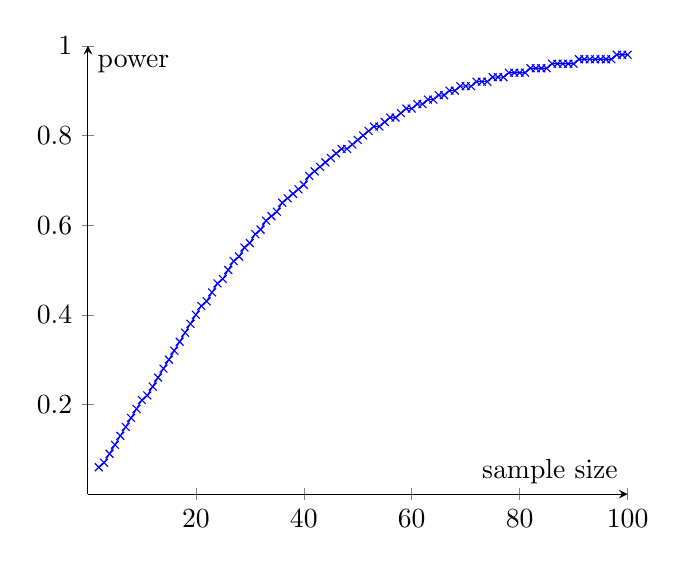
\begin{tikzpicture}
		\begin{axis}[
		xmin=0, xmax=100, xlabel=sample size,
		ymin=0, ymax=1, ylabel=power,
		samples=401,
		axis y line=middle,
		axis x line=middle,
		restrict y to domain=0:1,
		]
		\addplot[mark=x, blue] coordinates {
			(  2,0.06)
			(  3,0.07)
			(  4,0.09)
			(  5,0.11)
			(  6,0.13)
			(  7,0.15)
			(  8,0.17)
			(  9,0.19)
			( 10,0.21)
			( 11,0.22)
			( 12,0.24)
			( 13,0.26)
			( 14,0.28)
			( 15,0.30)
			( 16,0.32)
			( 17,0.34)
			( 18,0.36)
			( 19,0.38)
			( 20,0.40)
			( 21,0.42)
			( 22,0.43)
			( 23,0.45)
			( 24,0.47)
			( 25,0.48)
			( 26,0.50)
			( 27,0.52)
			( 28,0.53)
			( 29,0.55)
			( 30,0.56)
			( 31,0.58)
			( 32,0.59)
			( 33,0.61)
			( 34,0.62)
			( 35,0.63)
			( 36,0.65)
			( 37,0.66)
			( 38,0.67)
			( 39,0.68)
			( 40,0.69)
			( 41,0.71)
			( 42,0.72)
			( 43,0.73)
			( 44,0.74)
			( 45,0.75)
			( 46,0.76)
			( 47,0.77)
			( 48,0.77)
			( 49,0.78)
			( 50,0.79)
			( 51,0.80)
			( 52,0.81)
			( 53,0.82)
			( 54,0.82)
			( 55,0.83)
			( 56,0.84)
			( 57,0.84)
			( 58,0.85)
			( 59,0.86)
			( 60,0.86)
			( 61,0.87)
			( 62,0.87)
			( 63,0.88)
			( 64,0.88)
			( 65,0.89)
			( 66,0.89)
			( 67,0.90)
			( 68,0.90)
			( 69,0.91)
			( 70,0.91)
			( 71,0.91)
			( 72,0.92)
			( 73,0.92)
			( 74,0.92)
			( 75,0.93)
			( 76,0.93)
			( 77,0.93)
			( 78,0.94)
			( 79,0.94)
			( 80,0.94)
			( 81,0.94)
			( 82,0.95)
			( 83,0.95)
			( 84,0.95)
			( 85,0.95)
			( 86,0.96)
			( 87,0.96)
			( 88,0.96)
			( 89,0.96)
			( 90,0.96)
			( 91,0.97)
			( 92,0.97)
			( 93,0.97)
			( 94,0.97)
			( 95,0.97)
			( 96,0.97)
			( 97,0.97)
			( 98,0.98)
			( 99,0.98)
			(100,0.98)
		};
		\end{axis}
		\end{tikzpicture}
\end{center}

There are a many number of statistical tests for assessing normality: \person{Shapiro-Wilk} test, \person{Kolmogorov-Smirnov} test, \person{Jacque-Bera} test, etc. The \person{Shapiro-Wilk} test ($n<50$) can be used to verify whether data come from a normal distribution: \\
$H_0$: sample data are not significantly different than a normal population. \\
$H_A$: sample data are significantly different than a normal population. \\
P-value $>0.05$ mean the data are normal \\
P-value $<0.05$ mean the data are not normal \\
\person{Monte Carlo} simulations proved the efficiency of \person{Shapiro-Wilk} test. It s preferable that normality is assessed visually as well! The \person{Kolmogorov-Smirnov} non-parametric test ($n>50$) examines if scores are likely to follow some distribution in some population (not necessarily normal).
\subsection{Likelihood ratio test}

In some cases we need to perform a hypothesis test to compare two models: big "general" model ($M_B$) and small "simple" model ($M_S$) nested into the bigger model. \\
$H_0$: $M_S$ fits the data \\
$H_A$: $M_S$ does not fit the data and $M_B$ should be used instead. \\

We need to verify if $M_B$ fits the data significantly better.
\begin{itemize}
	\item \textbf{Measure how well a model fits the data:} The fit of any model can be described by the maximum possible likelihood for that model:
	\begin{align}
		L(M) = \max\{P(data\vert model)\}\notag
	\end{align}
	Calculate the maximum likelihood estimates for all unknown parameters and insert them into the likelihood function.
	\item \textbf{Work out the \begriff{likelihood ratio}:} 
	\begin{align}
		R = \frac{L(M_B)}{L(M_S)} \ge 1\notag
	\end{align}
	Big values of $R$ suggests that $M_S$ does not fit as well as $M_B$.
	\item \textbf{Work out log of likelihood ratio:} 
	\begin{align}
		\log(R) = l(M_B) - l(M_S) \ge 0\notag
	\end{align}
	Big values of $R$ suggests that $M_S$ does not fit as well as $M_B$.
\end{itemize}

\begin{example}
	There are a number of defective items on  a production line in 20 days that follow \person{Poisson}($\lambda$) distribution: 1, 2, 3, 4, 2, 3, 2, 5, 5, 2, 4, 3, 5, 1, 2, 4, 0, 2, 2, 6. \\
	$M_S$: the sample comes from \person{Poission}(2) \\
	$M_B$: the sample comes from \person{Poission}($\lambda$) \\
\end{example}

\begin{example}
	Clinical records give the survival time for 30 people: 9.73,5.56, 4.28, 4.87, 1.55, 6.20, 1.08, 7.17, 28.65, 6.10, 16.16, 9.92, 2.40, 6.19. In a clinical trial of a new drug treatment 20 people had survival times of: 22.07, 12.47, 6.42, 8.15, 0.64, 20.04, 17.49, 2.22, 3.00. Is there any difference in survival times for those using the new drug? \\
	$M_S$: Both examples come from the same exponential($\lambda$) distribution. \\
	$M_B$: The first sample comes from exponential($\lambda_1$) and the second sample from exponential($\lambda_2$).
\end{example}

\begin{definition}
	If the data come from $L(M_S)$, and $L(M_B)$ has $k$ more parameters than $L(M_S)$ then
	\begin{align}
		X^2 &= 2\log(R) \notag \\
		&= 2\big(l(M_B) - l(M_S)\big) \notag \\
		&\approx \chi^2(k \text{ degrees of freedom}) \notag
	\end{align}
\end{definition}

The main steps for the likelihood ratio test are:
\begin{enumerate}[label=\textbf{\arabic*.}]
	\item Work out maximum likelihood estimates of all unknown parameters in $M_S$.
	\item Work out maximum likelihood estimates of all unknown parameters in $M_B$.
	\item Evaluate the test statistic: $\chi^2 = 2\big(l(M_B) - l(M_S)\big)$
	\item The degrees of freedom for the test are the difference between the numbers of unknown parameters in two models. The p-value for the test is the upper tail probability of the $\chi^2(k \text{ degrees of freedom})$ distribution given the test statistic.
	\item Interpret the p-value: small values give evidence that the null hypothesis ($M_S$ model) does not hold.
\end{enumerate}

\begin{example}
	There are a number of defective items on  a production line in 20 days that follow \person{Poisson}($\lambda$) distribution: 1, 2, 3, 4, 2, 3, 2, 5, 5, 2, 4, 3, 5, 1, 2, 4, 0, 2, 2, 6.
	\begin{center}
		$\begin{array}{ccp{4cm}|p{7cm}}
		&&null hypothesis & $H_0$: $\lambda = 2$ small model $M_S$ \\
		\cline{3-4}
		&&alternative hypothesis & $H_A$: $\lambda \neq 2$ big model $M_B$\\
		\cline{3-4}
		&&log-likelihood for the Poisson distribution & $l(\lambda) = \left(\sum_{i=1}^{20} x_i\right)\log(\lambda) - n\lambda$ \\
		\cline{3-4}
		\multirow{3.7}{3mm}{$M_B$}& \ldelim\{{3.5}{2mm}  & MLE for the unknown parameter& $\hat{\lambda} = \frac{\sum x_i}{n} = 2.9$ \\ \cline{3-4}
		&  & Maximum possible value for the log-likelihood & $l(M_B) = 58\log(2.9) - 20\cdot 2.9 = 3.7532$ \\ \cline{3-4}
		\multirow{3.7}{3mm}{$M_S$}& \ldelim\{{3.5}{2mm}  & MLE for the unknown parameter& no unknown parameter \\ \cline{3-4}
		&  & Maximum possible value for the log-likelihood & $l(M_S) = 58\log(2) - 20\cdot 2 = 0.2025$ \\ \cline{3-4}
		&&Likelihood ratio test & $\chi^2 = 2\big(l(M_B) - l(M_S)\big) = 7.101$ \\
		\cline{3-4}
		&&\multicolumn{2}{p{11cm}}{It should be compared to $\chi^2(1\text{ degree of freedom})$ since the difference in unknown parameters is equal to 1.} \\
		\cline{3-4}
		&&p-value & The p-value is 0.008 (the upper tail probability above 7.101) \\
		\cline{3-4}
		&&Interpreting p-value & The p-value is very small and we can conclude that there is  strong evidence that $M_B$ fits the data better than $M_S$: $\lambda\neq 2$.
		\end{array}$
	\end{center}
	\begin{center}
		\begin{tikzpicture}[scale=0.9]
		\begin{axis}[
		xmin=0, xmax=10, xlabel=$x$,
		ymin=0, ymax=1, ylabel=$y$,
		samples=50,
		axis y line=middle,
		axis x line=middle,
		domain=0:10,
		restrict y to domain=0:1,
		]
		\addplot[name path=f,blue] {exp(-x/2)/(sqrt(2*pi) * sqrt(x))};
		\path[name path=axis] (axis cs:7.101,0) -- (axis cs:10,0);
		\addplot [thick,color=blue,fill=blue,fill opacity=0.3] fill between[of=f and axis,soft clip={domain=7.101:10},];
		\draw [dotted] (axis cs:7.101,0) -- (axis cs:7.101,0.6);
		\node at (axis cs:8.5,0.4) (a) {p-value};
		\draw (axis cs:8.5, 0.36) -- (axis cs: 7.5,0.0002);
		\end{axis}
		\end{tikzpicture}
		\begin{tikzpicture}[scale=0.9]
		\begin{axis}[
		xmin=6, xmax=10, xlabel=$x$,
		ymin=0, ymax=0.01, ylabel=$y$,
		samples=50,
		axis y line=middle,
		axis x line=middle,
		domain=0:10,
		restrict y to domain=0:0.01,
		]
		\addplot[name path=f,blue] {exp(-x/2)/(sqrt(2*pi) * sqrt(x))};
		\path[name path=axis] (axis cs:7.101,0) -- (axis cs:10,0);
		\addplot [thick,color=blue,fill=blue,fill opacity=0.3] fill between[of=f and axis,soft clip={domain=7.101:10},];
		\draw [dotted] (axis cs:7.101,0) -- (axis cs:7.101,0.006);
		\node at (axis cs:8.5,0.006) (a) {p-value};
		\draw (axis cs:8.5, 0.0056) -- (axis cs: 7.5,0.002);
		\end{axis}
		\end{tikzpicture}
	\end{center}
\end{example}

A \begriff{two-sample t-test} should be used to compare group means when you have independent samples. A \begriff{paired t-test} is needed when each sampled item in one group is associated with an item sampled from the other group.

\subsection{Two-sample t-test}

We can carry out a hypothesis test to verify if the two means are equal: \\
$H_0$: $\mu_1 = \mu_2$ \\
$H_A$: $\mu_1\neq\mu_2$ (The corresponding one-tailed alternative also holds.)

\begin{definition}
	If $\bar{x_1}$ and $\bar{x_2}$ come from Normal($\mu_1,\sigma$) and Normal($\mu_2,\sigma$) with sample sizes $n_1$ and $n_2$ then
	\begin{align}
		T = \frac{\bar{x_1}-\bar{x_2}}{\SE(\bar{x_1}-\bar{x_2})} \approx t(n_1+n_2-2\text{ degrees of freedom})\notag
	\end{align}
	provided $\mu_1=\mu_2$. For relatively large sample sizes (Central Limit Theorem) we can use Z-test instead of t-test.
\end{definition} 

\begin{example}
	A botanist is interested in comparing the growth response of dwarf pea stems to two different levels of the hormone indoleacetic acid (IAA). The botanist measured the growth of pea stem segments in millimetres for $0.5\cdot 10^{-4}$ IAA level: 0.8, 1.8, 1.0, 0.1, 0.9, 1.7, 1.0, 1.4, 0.9, 1.2, 0.5 and for $10^{-4}$ IAA level: 1.0, 1.8, 0.8, 2.5, 1.6, 1.4, 2.6, 1.9, 1.3, 2.0, 1.1, 1.2. Test whether the larger hormone concentration results in greater growth of the pea plants.
	\begin{center}
		\begin{tabular}{p{4cm}|p{7cm}}
			independent samples & $n_x = 11$, $n_y=12$ \\
			\hline
			Null hypothesis & $H_0$: $\mu_x=\mu_y$ \\
			\hline
			Alternative hypothesis & $H_A$: $\mu_x < \mu_y$ \\
			\hline
			The \begriff{pooled estimate} assumes that the variance is the same in both groups & $s^2 = \frac{10s_x^2 + 11s_y^2}{21} = 0.2896$ \\
			\hline
			test statistic & $t=\frac{1.027-1.6}{\sqrt{0.2896(\frac{1}{11} + \frac{1}{12})}} = -2.5496$ \\
			\hline
			p-value for 21 degrees of freedom in t-distribution & $P(t\le -2.5496) = 0.0093$ \\
			\hline
			Interpretation & There is very strong evidence that the mean growth of the peas is higher at the higher hormone concentration.
		\end{tabular}
	\end{center}
	\begin{center}
		\begin{tikzpicture}
		\begin{axis}[
		xmin=-3, xmax=3, xlabel=$x$,
		ymin=0, ymax=1, ylabel=$y$,
		samples=400,
		axis y line=middle,
		axis x line=middle,
		domain=-3:3,
		restrict y to domain=0:1,
		]
		\addplot[name path=f,blue] {(1.38087*10^(14))/((x^2+21)^(11))};
		\path[name path=axis] (axis cs:-3,0) -- (axis cs:-2.5496,0);
		\addplot [thick,color=blue,fill=blue,fill opacity=0.3] fill between[of=f and axis,soft clip={domain=-3:-2.5496},];
		\draw [dotted] (axis cs:-2.5496,0) -- (axis cs:-2.5496,0.6);
		\node at (axis cs:-1.7,0.3) (a) {p-value};
		\draw (axis cs:-1.7, 0.26) -- (axis cs: -2.7,0.01);
		\end{axis}
		\end{tikzpicture}
	\end{center}
\end{example}

\begin{*anmerkung}[pooled variance]
	In statistics, pooled variance (also known as combined, composite, or overall variance) is a method for estimating variance of several different populations when the mean of each population may be different, but one may assume that the variance of each population is the same. The numerical estimate resulting from the use of this method is also called the pooled variance.
	
	Under the assumption of equal population variances, the pooled sample variance provides a higher precision estimate of variance than the individual sample variances. This higher precision can lead to increased statistical power when used in statistical tests that compare the populations, such as the t-test.
	\begin{align}
		s^2 = \frac{\sum_{i=1}^k (n_i-1)s_i^2}{\sum_{i=1}^k (n_i-1)} \notag
	\end{align}
	Adapted from \url{https://en.wikipedia.org/wiki/Pooled_variance}.
\end{*anmerkung}

\subsection{Paired t-test}

Testing whether two paired measurements $X$ and $Y$ have equal means is done in terms of the difference $D=Y-X$. The hypothesis \\
$H_0$: $\mu_x = \mu_y$ \\
$H_A$: $\mu_x\neq \mu_y$ \\
can be re-written as \\
$H_0$: $\mu_d=0$ \\
$H_A$: $\mu_d\neq 0$. \\
This can reduce the paired data set to a univariate data set of differences. The hypothesis can be assigned using t-test:
\begin{align}
	t = \frac{\bar{d}-0}{\frac{s_d}{\sqrt{n}}} \notag
\end{align}
Z-test can be used for relatively large sample sizes.

\begin{example}
	A researcher studying congenital heard disease wants to compare the development of cyanotic children with normal children. Among the measurement of interest is the age at which the children speak their first word.
	\begin{center}
		\begin{tabular}{c|cc|c}
			\textbf{pair of siblings} & \textbf{cyanotic sibling} & \textbf{normal sibling} & \textbf{difference} \\
			\hline
			1 & 11.8 & 9.8 & 2.0 \\
			2 & 20.8 & 16.5 & 4.3 \\
			3 & 14.5 & 14.5 & 0.0 \\
			4 & 9.5 & 15.2 & -5.7 \\
			5 & 13.5 & 11.8 & 1.7 \\
			6 & 22.6 & 12.2 & 10.4 \\
			7 & 11.1 & 15.2 & -4.1 \\
			8 & 14.9 & 15.6 & -0.7 \\
			9 & 16.5 & 17.2 & -0.7 \\
			10 & 16.5 & 10.5 & 6.0 \\
		\end{tabular}
	\end{center}
	The researcher wants to test whether cyanotic children speak their first word later on average than children without the disease.
	\begin{center}
		\begin{tabular}{p{4cm}|p{7cm}}
			Null hypothesis & $H_0$: $\mu_d = 0$ \\
			\hline
			Alternative hypothesis & $H_A$: $\mu_d > 0$ \\
			\hline
			test statistic & $t = \frac{\bar{d}-0}{\frac{s_d}{\sqrt{n}}} = 0.8802$ \\
			\hline
			Interpretation & The p-value is well above zero (0.1997), so there is no evidence that the cyanotic children learn to speak later.
		\end{tabular}
	\end{center}
	\begin{center}
		\begin{tikzpicture}
		\begin{axis}[
		xmin=-3, xmax=3, xlabel=$x$,
		ymin=0, ymax=1, ylabel=$y$,
		samples=400,
		axis y line=middle,
		axis x line=middle,
		domain=-3:3,
		restrict y to domain=0:1,
		]
		\addplot[name path=f,blue] {(984375)/(8*(x^2+10)^(5.5))};
		\path[name path=axis] (axis cs:0.8802,0) -- (axis cs:3,0);
		\addplot [thick,color=blue,fill=blue,fill opacity=0.3] fill between[of=f and axis,soft clip={domain=0.8802:3},];
		\draw [dotted] (axis cs:0.8802,0) -- (axis cs:0.8802,0.6);
		\node at (axis cs:1.7,0.4) (a) {p-value};
		\draw (axis cs:1.7, 0.36) -- (axis cs: 1.2,0.08);
		\end{axis}
		\end{tikzpicture}
	\end{center}
\end{example}

\begin{example}
	The blood pressure of 15 college-aged woman was measured before starting to take the pill and after 6 months of use.
	\begin{center}
		\begin{tabular}{c|cc}
			 & \multicolumn{2}{c}{\textbf{blood pressure}} \\
			 \textbf{subject} & \textbf{before pill} & \textbf{after pill} \\
			 \hline
			 1 & 70 & 68 \\
			 2 & 80 & 72 \\
			 3 & 72 & 62 \\
			 4 & 76 & 70 \\
			 5 & 76 & 58 \\
			 6 & 76 & 66 \\
			 7 & 72 & 68 \\
			 8 & 78 & 52 \\
			 9 & 82 & 64 \\
			 10 & 64 & 72 \\
			 11 & 74 & 74 \\
			 12 & 92 & 60 \\
			 13 & 74 & 74 \\
			 14 & 68 & 72 \\
			 15 & 84 & 74 \\
		\end{tabular}
	\end{center}
	A two-tailed test is used as the pill might either increase or decrease blood pressure.
	\begin{center}
		\begin{tabular}{p{4cm}|p{7cm}}
			Null hypothesis & $H_0$: $\mu_d = 0$ \\
			\hline
			Alternative hypothesis & $H_A$: $\mu_d \neq 0$ \\
			\hline
			test statistic & $t = \frac{\bar{d}-0}{\frac{s_d}{\sqrt{n}}} = -3.1054$ \\
			\hline
			Interpretation & The p-value (0.0072) is very small that gives strong evidence that the blood pressure has changed. The negative t-value suggests that the blood pressure has decreased.
		\end{tabular}
	\end{center}
	\begin{center}
		\begin{tikzpicture}[scale=0.9]
		\begin{axis}[
		xmin=-4, xmax=4, xlabel=$x$,
		ymin=0, ymax=1, ylabel=$y$,
		samples=400,
		axis y line=middle,
		axis x line=middle,
		domain=-4:4,
		restrict y to domain=0:1,
		]
		\addplot[name path=f,blue] {(116640000000*sqrt(15))/(143*pi*(x^2+15)^(8))};
		\path[name path=axis] (axis cs:-4,0) -- (axis cs:-3.1054,0);
		\addplot [thick,color=blue,fill=blue,fill opacity=0.3] fill between[of=f and axis,soft clip={domain=-4:-3.1054},];
		\draw [dotted] (axis cs:-3.1054,0) -- (axis cs:-3.1054,0.6);
		\node at (axis cs:-2.2,0.4) (a) {p-value};
		\draw (axis cs:-2.2, 0.36) -- (axis cs: -3.2,0.001);
		\end{axis}
		\end{tikzpicture}
		\begin{tikzpicture}[scale=0.9]
		\begin{axis}[
		xmin=-4, xmax=-2, xlabel=$x$,
		ymin=0, ymax=0.1, ylabel=$y$,
		samples=400,
		axis y line=middle,
		axis x line=middle,
		domain=-4:-2,
		restrict y to domain=0:0.1,
		]
		\addplot[name path=f,blue] {(116640000000*sqrt(15))/(143*pi*(x^2+15)^(8))};
		\path[name path=axis] (axis cs:-4,0) -- (axis cs:-3.1054,0);
		\addplot [thick,color=blue,fill=blue,fill opacity=0.3] fill between[of=f and axis,soft clip={domain=-4:-3.1054},];
		\draw [dotted] (axis cs:-3.1054,0) -- (axis cs:-3.1054,0.06);
		\node at (axis cs:-3.6,0.05) (a) {p-value};
		\draw (axis cs:-3.6, 0.046) -- (axis cs: -3.2,0.003);
		\end{axis}
		\end{tikzpicture}
	\end{center}
\end{example}
\pagebreak
\section{Bootstrapping}
\subsection{A word of warning}

The limitation of the bootstrap is the assumption that the distribution of the data represented by one sample is an accurate estimate of the population distribution. If the sample does not reflect the population distribution, then the random sampling performed in the bootstrap procedure may add another level of sampling error, resulting in inaccurate statistical estimations.

It is important to get quality data that accurately reflects the population being sampled. The smaller the original sample, the less likely it is to accurately represent the entire population.

We use bootstrap if
\begin{itemize}
	\item we have a small but representative random sample or
	\item we have a not-normal distribution or aren't sure about it.
\end{itemize}

\subsection{Why to use it?}

In normal population the mean $\mu$ is the parameter that is most often estimated. But other parameters are possible too:
\begin{itemize}
	\item standard deviation
	\item interquartile range (upper quartile - lower quartile)
	\item median
	\item other percentiles (e.g. upper quartile)
\end{itemize}
These parameters can be estimated using the corresponding summary statistic from a random sample, but the error distribution may be difficult to obtain theoretically.

Resampling techniques are normally used to estimate parameters and confidence intervals from sample data when parametric test assumptions are not met or for small samples from non-normal distributions.
\begin{itemize}
	\item non-parametric bootstrap
	\item \textcolor{gray}{parametric bootstrap}
	\item \textcolor{gray}{Jackknife}
	\item \textcolor{gray}{permutation tests}
\end{itemize}
Non-parametric bootstrap means that only a random sample is known and no prior knowledge on the population density function.

\begin{example}
	Monthly rainfall in Dodoma, Tanzania has a skew distribution in some months. The distribution of a sample is provided below.
	
	\begin{center}
	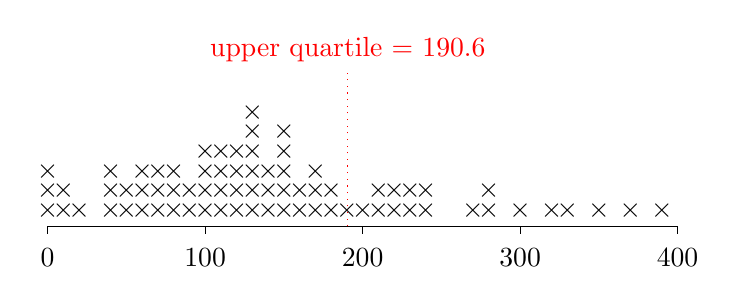
\begin{tikzpicture}
		\node at (0.00,0.25) (1) {$\times$};
		\node at (0.00,0.50) (1) {$\times$};
		\node at (0.00,0.75) (1) {$\times$};
		\node at (0.20,0.25) (1) {$\times$};
		\node at (0.20,0.50) (1) {$\times$};
		\node at (0.40,0.25) (1) {$\times$};
		\node at (0.80,0.25) (1) {$\times$};
		\node at (0.80,0.50) (1) {$\times$};
		\node at (0.80,0.75) (1) {$\times$};
		\node at (1.00,0.25) (1) {$\times$};
		\node at (1.00,0.50) (1) {$\times$};
		\node at (1.20,0.25) (1) {$\times$};
		\node at (1.20,0.50) (1) {$\times$};
		\node at (1.20,0.75) (1) {$\times$};
		\node at (1.40,0.25) (1) {$\times$};
		\node at (1.40,0.50) (1) {$\times$};
		\node at (1.40,0.75) (1) {$\times$};
		\node at (1.60,0.25) (1) {$\times$};
		\node at (1.60,0.50) (1) {$\times$};
		\node at (1.60,0.75) (1) {$\times$};
		\node at (1.80,0.25) (1) {$\times$};
		\node at (1.80,0.50) (1) {$\times$};
		\node at (2.00,0.25) (1) {$\times$};
		\node at (2.00,0.50) (1) {$\times$};
		\node at (2.00,0.75) (1) {$\times$};
		\node at (2.00,1.00) (1) {$\times$};
		\node at (2.20,0.25) (1) {$\times$};
		\node at (2.20,0.50) (1) {$\times$};
		\node at (2.20,0.75) (1) {$\times$};
		\node at (2.20,1.00) (1) {$\times$};
		\node at (2.40,0.25) (1) {$\times$};
		\node at (2.40,0.50) (1) {$\times$};
		\node at (2.40,0.75) (1) {$\times$};
		\node at (2.40,1.00) (1) {$\times$};
		\node at (2.60,0.25) (1) {$\times$};
		\node at (2.60,0.50) (1) {$\times$};
		\node at (2.60,0.75) (1) {$\times$};
		\node at (2.60,1.00) (1) {$\times$};
		\node at (2.60,1.25) (1) {$\times$};
		\node at (2.60,1.50) (1) {$\times$};
		\node at (2.80,0.25) (1) {$\times$};
		\node at (2.80,0.50) (1) {$\times$};
		\node at (2.80,0.75) (1) {$\times$};
		\node at (3.00,0.25) (1) {$\times$};
		\node at (3.00,0.50) (1) {$\times$};
		\node at (3.00,0.75) (1) {$\times$};
		\node at (3.00,1.00) (1) {$\times$};
		\node at (3.00,1.25) (1) {$\times$};
		\node at (3.20,0.25) (1) {$\times$};
		\node at (3.20,0.50) (1) {$\times$};
		\node at (3.40,0.25) (1) {$\times$};
		\node at (3.40,0.50) (1) {$\times$};
		\node at (3.40,0.75) (1) {$\times$};
		\node at (3.60,0.25) (1) {$\times$};
		\node at (3.60,0.50) (1) {$\times$};
		\node at (3.80,0.25) (1) {$\times$};
		\node at (4.00,0.25) (1) {$\times$};
		\node at (4.20,0.25) (1) {$\times$};
		\node at (4.20,0.50) (1) {$\times$};
		\node at (4.40,0.25) (1) {$\times$};
		\node at (4.40,0.50) (1) {$\times$};
		\node at (4.60,0.25) (1) {$\times$};
		\node at (4.60,0.50) (1) {$\times$};
		\node at (4.80,0.25) (1) {$\times$};
		\node at (4.80,0.50) (1) {$\times$};
		\node at (5.40,0.25) (1) {$\times$};
		\node at (5.60,0.25) (1) {$\times$};
		\node at (5.60,0.50) (1) {$\times$};
		\node at (6.00,0.25) (1) {$\times$};
		\node at (6.40,0.25) (1) {$\times$};
		\node at (6.60,0.25) (1) {$\times$};
		\node at (7.00,0.25) (1) {$\times$};
		\node at (7.40,0.25) (1) {$\times$};
		\node at (7.80,0.25) (1) {$\times$};
		
		\draw (0,0.05) -- (8,0.05);
		\draw (0,0.05) -- (0,-0.05);
		\draw (2,0.05) -- (2,-0.05);
		\draw (4,0.05) -- (4,-0.05);
		\draw (6,0.05) -- (6,-0.05);
		\draw (8,0.05) -- (8,-0.05);
		
		\node at (0,-0.35) (0) {0};
		\node at (2,-0.35) (0) {100};
		\node at (4,-0.35) (0) {200};
		\node at (6,-0.35) (0) {300};
		\node at (8,-0.35) (0) {400};
		
		\draw[red,dotted] (3.812,0.05) -- (3.812,2);
		\node[red] at (3.812,2.3) (up) {upper quartile = 190.6};
	\end{tikzpicture}
\end{center}
	
	If a normal distribution does not seem a reasonable model, an alternative is to treat the actual sample as the "population" for the simulation and take random samples with replacement from this sample. Such samples are called \begriff{bootstrap samples}. A simulation with these bootstrap samples can again show the error distribution and provide approximate values for the bias and standard error.
	
	\begin{center}
	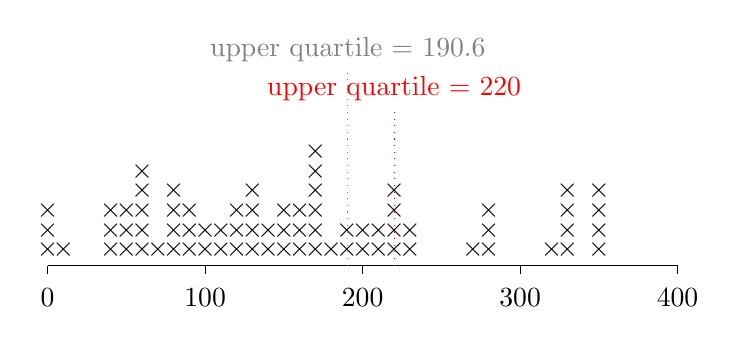
\begin{tikzpicture}
		\node at (0.00,0.25) (1) {$\times$};
		\node at (0.00,0.50) (1) {$\times$};
		\node at (0.00,0.75) (1) {$\times$};
		\node at (0.20,0.25) (1) {$\times$};
		\node at (0.80,0.25) (1) {$\times$};
		\node at (0.80,0.50) (1) {$\times$};
		\node at (0.80,0.75) (1) {$\times$};
		\node at (1.00,0.25) (1) {$\times$};
		\node at (1.00,0.50) (1) {$\times$};
		\node at (1.00,0.75) (1) {$\times$};
		\node at (1.20,0.25) (1) {$\times$};
		\node at (1.20,0.50) (1) {$\times$};
		\node at (1.20,0.75) (1) {$\times$};
		\node at (1.20,1.00) (1) {$\times$};
		\node at (1.20,1.25) (1) {$\times$};
		\node at (1.40,0.25) (1) {$\times$};
		\node at (1.60,0.25) (1) {$\times$};
		\node at (1.60,0.50) (1) {$\times$};
		\node at (1.60,0.75) (1) {$\times$};
		\node at (1.60,1.00) (1) {$\times$};
		\node at (1.80,0.25) (1) {$\times$};
		\node at (1.80,0.50) (1) {$\times$};
		\node at (1.80,0.75) (1) {$\times$};
		\node at (2.00,0.25) (1) {$\times$};
		\node at (2.00,0.50) (1) {$\times$};
		\node at (2.20,0.25) (1) {$\times$};
		\node at (2.20,0.50) (1) {$\times$};
		\node at (2.40,0.25) (1) {$\times$};
		\node at (2.40,0.50) (1) {$\times$};
		\node at (2.40,0.75) (1) {$\times$};
		\node at (2.60,0.25) (1) {$\times$};
		\node at (2.60,0.50) (1) {$\times$};
		\node at (2.60,0.75) (1) {$\times$};
		\node at (2.60,1.00) (1) {$\times$};
		\node at (2.80,0.25) (1) {$\times$};
		\node at (2.80,0.50) (1) {$\times$};
		\node at (3.00,0.25) (1) {$\times$};
		\node at (3.00,0.50) (1) {$\times$};
		\node at (3.00,0.75) (1) {$\times$};
		\node at (3.20,0.25) (1) {$\times$};
		\node at (3.20,0.50) (1) {$\times$};
		\node at (3.20,0.75) (1) {$\times$};
		\node at (3.40,0.25) (1) {$\times$};
		\node at (3.40,0.50) (1) {$\times$};
		\node at (3.40,0.75) (1) {$\times$};
		\node at (3.40,1.00) (1) {$\times$};
		\node at (3.40,1.25) (1) {$\times$};
		\node at (3.40,1.50) (1) {$\times$};
		\node at (3.60,0.25) (1) {$\times$};
		\node at (3.80,0.25) (1) {$\times$};
		\node at (3.80,0.50) (1) {$\times$};
		\node at (4.00,0.25) (1) {$\times$};
		\node at (4.00,0.50) (1) {$\times$};
		\node at (4.20,0.25) (1) {$\times$};
		\node at (4.20,0.50) (1) {$\times$};
		\node at (4.40,0.25) (1) {$\times$};
		\node at (4.40,0.50) (1) {$\times$};
		\node at (4.40,0.75) (1) {$\times$};
		\node at (4.40,1.00) (1) {$\times$};
		\node at (4.60,0.25) (1) {$\times$};
		\node at (4.60,0.50) (1) {$\times$};
		\node at (5.40,0.25) (1) {$\times$};
		\node at (5.60,0.25) (1) {$\times$};
		\node at (5.60,0.50) (1) {$\times$};
		\node at (5.60,0.75) (1) {$\times$};
		\node at (6.40,0.25) (1) {$\times$};
		\node at (6.60,0.25) (1) {$\times$};
		\node at (6.60,0.50) (1) {$\times$};
		\node at (6.60,0.75) (1) {$\times$};
		\node at (6.60,1.00) (1) {$\times$};
		\node at (7.00,0.25) (1) {$\times$};
		\node at (7.00,0.50) (1) {$\times$};
		\node at (7.00,0.75) (1) {$\times$};
		\node at (7.00,1.00) (1) {$\times$};
		
		\draw (0,0.05) -- (8,0.05);
		\draw (0,0.05) -- (0,-0.05);
		\draw (2,0.05) -- (2,-0.05);
		\draw (4,0.05) -- (4,-0.05);
		\draw (6,0.05) -- (6,-0.05);
		\draw (8,0.05) -- (8,-0.05);
		
		\node at (0,-0.35) (0) {0};
		\node at (2,-0.35) (0) {100};
		\node at (4,-0.35) (0) {200};
		\node at (6,-0.35) (0) {300};
		\node at (8,-0.35) (0) {400};
		
		\draw[gray,dotted] (3.812,0.05) -- (3.812,2.5);
		\node[gray] at (3.812,2.8) (up) {upper quartile = 190.6};
		\draw[red,dotted] (4.4,0.05) -- (4.4,2);
		\node[red] at (4.4,2.3) (up) {upper quartile = 220};
	\end{tikzpicture}
\end{center}
	\begin{center}
	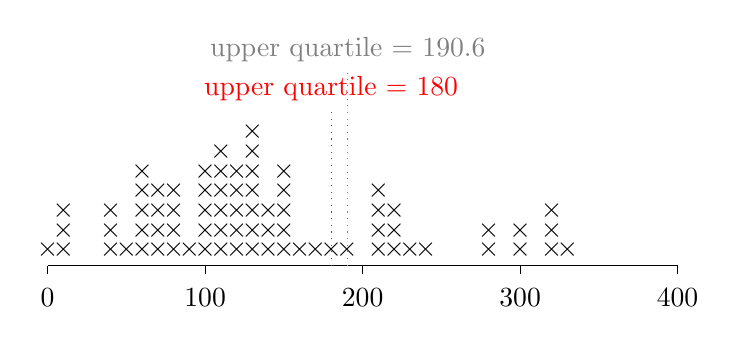
\begin{tikzpicture}
		\node at (0.00,0.25) (1) {$\times$};
		\node at (0.20,0.25) (1) {$\times$};
		\node at (0.20,0.50) (1) {$\times$};
		\node at (0.20,0.75) (1) {$\times$};
		\node at (0.80,0.25) (1) {$\times$};
		\node at (0.80,0.50) (1) {$\times$};
		\node at (0.80,0.75) (1) {$\times$};
		\node at (1.00,0.25) (1) {$\times$};
		\node at (1.20,0.25) (1) {$\times$};
		\node at (1.20,0.50) (1) {$\times$};
		\node at (1.20,0.75) (1) {$\times$};
		\node at (1.20,1.00) (1) {$\times$};
		\node at (1.20,1.25) (1) {$\times$};
		\node at (1.40,0.25) (1) {$\times$};
		\node at (1.40,0.50) (1) {$\times$};
		\node at (1.40,0.75) (1) {$\times$};
		\node at (1.40,1.00) (1) {$\times$};
		\node at (1.60,0.25) (1) {$\times$};
		\node at (1.60,0.50) (1) {$\times$};
		\node at (1.60,0.75) (1) {$\times$};
		\node at (1.60,1.00) (1) {$\times$};
		\node at (1.80,0.25) (1) {$\times$};
		\node at (2.00,0.25) (1) {$\times$};
		\node at (2.00,0.50) (1) {$\times$};
		\node at (2.00,0.75) (1) {$\times$};
		\node at (2.00,1.00) (1) {$\times$};
		\node at (2.00,1.25) (1) {$\times$};
		\node at (2.20,0.25) (1) {$\times$};
		\node at (2.20,0.50) (1) {$\times$};
		\node at (2.20,0.75) (1) {$\times$};
		\node at (2.20,1.00) (1) {$\times$};
		\node at (2.20,1.25) (1) {$\times$};
		\node at (2.20,1.50) (1) {$\times$};
		\node at (2.40,0.25) (1) {$\times$};
		\node at (2.40,0.50) (1) {$\times$};
		\node at (2.40,0.75) (1) {$\times$};
		\node at (2.40,1.00) (1) {$\times$};
		\node at (2.40,1.25) (1) {$\times$};
		\node at (2.60,0.25) (1) {$\times$};
		\node at (2.60,0.50) (1) {$\times$};
		\node at (2.60,0.75) (1) {$\times$};
		\node at (2.60,1.00) (1) {$\times$};
		\node at (2.60,1.25) (1) {$\times$};
		\node at (2.60,1.50) (1) {$\times$};
		\node at (2.60,1.75) (1) {$\times$};
		\node at (2.80,0.25) (1) {$\times$};
		\node at (2.80,0.50) (1) {$\times$};
		\node at (2.80,0.75) (1) {$\times$};
		\node at (3.00,0.25) (1) {$\times$};
		\node at (3.00,0.50) (1) {$\times$};
		\node at (3.00,0.75) (1) {$\times$};
		\node at (3.00,1.00) (1) {$\times$};
		\node at (3.00,1.25) (1) {$\times$};
		\node at (3.20,0.25) (1) {$\times$};
		\node at (3.40,0.25) (1) {$\times$};
		\node at (3.60,0.25) (1) {$\times$};
		\node at (3.80,0.25) (1) {$\times$};
		\node at (4.20,0.25) (1) {$\times$};
		\node at (4.20,0.50) (1) {$\times$};
		\node at (4.20,0.75) (1) {$\times$};
		\node at (4.20,1.00) (1) {$\times$};
		\node at (4.40,0.25) (1) {$\times$};
		\node at (4.40,0.50) (1) {$\times$};
		\node at (4.40,0.75) (1) {$\times$};
		\node at (4.60,0.25) (1) {$\times$};
		\node at (4.80,0.25) (1) {$\times$};
		\node at (5.60,0.25) (1) {$\times$};
		\node at (5.60,0.50) (1) {$\times$};
		\node at (6.00,0.25) (1) {$\times$};
		\node at (6.00,0.50) (1) {$\times$};
		\node at (6.40,0.25) (1) {$\times$};
		\node at (6.40,0.50) (1) {$\times$};
		\node at (6.40,0.75) (1) {$\times$};
		\node at (6.60,0.25) (1) {$\times$};
		
		\draw (0,0.05) -- (8,0.05);
		\draw (0,0.05) -- (0,-0.05);
		\draw (2,0.05) -- (2,-0.05);
		\draw (4,0.05) -- (4,-0.05);
		\draw (6,0.05) -- (6,-0.05);
		\draw (8,0.05) -- (8,-0.05);
		
		\node at (0,-0.35) (0) {0};
		\node at (2,-0.35) (0) {100};
		\node at (4,-0.35) (0) {200};
		\node at (6,-0.35) (0) {300};
		\node at (8,-0.35) (0) {400};
		
		\draw[gray,dotted] (3.812,0.05) -- (3.812,2.5);
		\node[gray] at (3.812,2.8) (up) {upper quartile = 190.6};
		\draw[red,dotted] (3.6,0.05) -- (3.6,2);
		\node[red] at (3.6,2.3) (up) {upper quartile = 180};
	\end{tikzpicture}
\end{center}
\end{example}

\subsection{Bootstrap distribution}

The standard error of a statistic is the standard deviation of the sample statistic. The standard error can be calculated as the standard deviation of the sampling distribution.

Bootstrap sample is a random sample taken with replacement from the original sample, of the same size as the original sample. A bootstrap statistic is the statistic computed on a bootstrap sample. A bootstrap distribution is the distribution of many bootstrap statistics. The standard error of a statistic can be estimated using the standard deviation of the bootstrap distribution.

Let $\hat{\theta}$ a statistic calculated from a sample ($\hat{\theta} = \bar{x}$). We draw $r$ observations with replacement to create a bootstrap sample and calculate the statistic $\hat{\theta}^\ast$ for this sample.
\begin{itemize}
	\item \textbf{bootstrap standard error:} the sample standard deviation of the bootstrap distribution:
	\begin{align}
		\SE_b = \sqrt{\frac{\sum (\hat{\theta}^\ast_b - \bar{\theta}^\ast)^2}{B-1}} \notag
	\end{align}
	where $B$ is the number of bootstrap replications (usually $B>10000$)
	\item \textbf{bootstrap bias:} $\bar{\theta}^\ast-\hat{\theta}$
	\item \textbf{bootstrap confidence intervals:} bootstrap percentile interval, t confidence interval with bootstrap standard error, bootstrap t-interval, etc.
\end{itemize}

\subsection{Bootstrap methods}
\pagebreak
\section{Linear models (Simple linear regression)}
\begin{example}
	Suppose a chemical reaction produces higher yields of a product, the higher the ambient temperature
	\begin{center}
		\begin{tikzpicture}
		\begin{axis}[
		xmin=50, xmax=100, xlabel=temperature,
		ymin=100, ymax=250, ylabel=yiels,
		samples=400,
		axis x line=bottom,
		axis y line=left,
		domain=50:100,
		]
		\addplot[mark=x,only marks] coordinates {
			(50,120)
			(53,115)
			(54,125)
			(55,119)
			(56,120)
			(59,140)
			(62,145)
			(64,143)
			(67,147)
			(71,157)
			(72,160)
			(74,175)
			(75,159)
			(76,177)
			(79,180)
			(80,185)
			(82,182)
			(85,185)
			(87,188)
			(89,200)
			(93,195)
			(94,203)
			(95,204)
			(97,212)
		};
		\end{axis}
		\end{tikzpicture}
	\end{center}
	Simple linear regression is what we can use to investigate if a relationship between two variables exists when we don't know about the underlying process. We model a linear relationship between two variables and
	\begin{enumerate}[label=(\alph*)]
		\item quantify this pattern before
		\item testing if we can believe it
	\end{enumerate}
\end{example}

\subsection{Structure of simple linear regression models}

\begin{definition}[simple linear regression]
	For $n$ observed data pairs $\{(x_i,Y_i)\mid i=1,...,n\}$ \begriff{simple linear regression} assumes we have the relationship
	\begin{align}
		Y_i = \beta_0 + \beta_1x_i + \epsilon_i\notag
	\end{align}
	$Y$ is called the \begriff{respose variable} and $x$ the \begriff{explainatory variable}. $\beta_0$ and $\beta_1$ are \begriff{model parameters}. $\epsilon_i$ are error terms (spread around the regression line) and crucially, we assume $\epsilon_i\overset{i.i.d}{\sim}Normal(0,\sigma)$ in simple linear regression.
\end{definition}

\begin{definition}[alternative representations for simple linear regression models]
	\begin{enumerate}[label=(\alph*)]
		\item algebraic notation:
		\begin{align}
			Y_1 &= \beta_0 + \beta_1x_1 + \epsilon_1 \notag \\
			Y_2 &= \beta_0 + \beta_1x_2 + \epsilon_2 \notag \\
			\vdots  \notag \\
			Y_n &= \beta_0 + \beta_1x_n + \epsilon_n \notag
		\end{align}
		\item Matrix notation:
		\begin{align}
			Y = \beta X + \epsilon \notag 
		\end{align}
		Because of the error term $\epsilon$, the response $Y$ is a random variable. So, $Y_i = E(Y_i)+\epsilon_i = \beta_0+\beta_1x_i+\epsilon_i$ and thus $E(Y_i) = \beta_0+\beta_1x_i$. This leads to the following notation
		\item Random variable notation: 
		\begin{align}
			Y_i &\overset{i.i.d}{\sim}Normal(\beta_0+\beta_1x_i,\sigma) \notag \\
			Y &\sim Normal(X\beta,\mathbbm{1}\sigma) \notag
		\end{align}
		Since the mean of the response is a linear function of the explanatory variables, there are often called simple linear models.
	\end{enumerate}
\end{definition}

Given data, we want to estimate the parameters of the model. In this course, we always use Maximum Likelihood Estimation (MLE). That means, we find parameter values that maximise the likelihood of our model. The likelihood for an simple linear model is
\begin{align}
	L(\beta\mid X) = \prod_{i=1}^{n} f_{Normal}(Y_i,\mu=\beta_0+\beta_1x_i,\sigma) \notag
\end{align}
where $f_{Normal}$ is the PDF for the normal distribution with mean $\mu=\beta_0+\beta_1x_i$ and standard deviation $\sigma$ evaluated at $Y_i$. For linear models, it has been shown that MLE is equivalent to Ordinary Least Squares (OLS). For linear models exact equations for these parameter estimates exist
\begin{align}
	\hat{\beta} &= (X^TX)^{-1}X^TY \notag \\
	\hat{\sigma}^2 &= \frac{1}{n-2}(Y-X\hat{\beta})^T(Y-X\hat{\beta})\notag
\end{align}
Fitted values for the response are: $\hat{Y} = X\hat{\beta}$

\begin{center}
	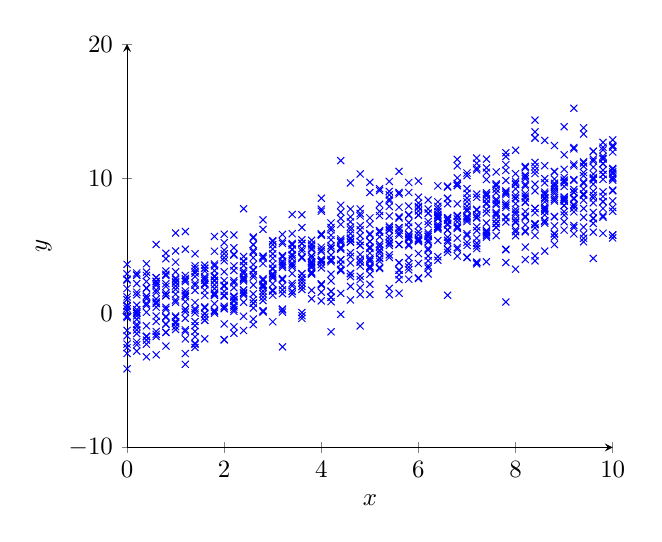
\begin{tikzpicture}[scale=0.9]
	\begin{axis}[
	xmin=0, xmax=10, xlabel=$x$,
	ymin=-10, ymax=20, ylabel=$y$,
	samples=400,
	axis x line=bottom,
	axis y line=left,
	domain=0:-10,
	]
	\addplot[mark=x,only marks, blue] coordinates {
		(0.00,-3.01)
		(0.00,3.62)
		(0.00,-0.23)
		(0.00,2.45)
		(0.00,0.99)
		(0.00,1.82)
		(0.00,-2.31)
		(0.00,2.52)
		(0.00,2.91)
		(0.00,-4.15)
		(0.00,-0.35)
		(0.00,-1.30)
		(0.00,0.31)
		(0.00,-1.70)
		(0.00,0.56)
		(0.00,1.19)
		(0.00,0.49)
		(0.00,-0.24)
		(0.00,-2.58)
		(0.00,0.12)
		(0.20,-0.84)
		(0.20,-2.36)
		(0.20,0.09)
		(0.20,-0.22)
		(0.20,0.58)
		(0.20,2.18)
		(0.20,1.35)
		(0.20,2.81)
		(0.20,-1.26)
		(0.20,-1.53)
		(0.20,0.01)
		(0.20,2.97)
		(0.20,2.81)
		(0.20,-0.05)
		(0.20,-0.99)
		(0.20,-2.84)
		(0.20,1.54)
		(0.20,0.25)
		(0.20,-2.16)
		(0.20,-0.47)
		(0.40,-3.26)
		(0.40,1.26)
		(0.40,0.05)
		(0.40,3.66)
		(0.40,-2.32)
		(0.40,2.34)
		(0.40,0.69)
		(0.40,0.57)
		(0.40,1.83)
		(0.40,2.79)
		(0.40,-1.74)
		(0.40,3.04)
		(0.40,-2.02)
		(0.40,-1.75)
		(0.40,-0.95)
		(0.40,1.87)
		(0.40,-1.74)
		(0.40,1.07)
		(0.40,1.22)
		(0.40,0.71)
		(0.60,1.71)
		(0.60,-1.75)
		(0.60,2.62)
		(0.60,0.83)
		(0.60,2.06)
		(0.60,-1.37)
		(0.60,0.70)
		(0.60,2.36)
		(0.60,2.63)
		(0.60,0.43)
		(0.60,-3.11)
		(0.60,-1.59)
		(0.60,1.04)
		(0.60,2.19)
		(0.60,1.53)
		(0.60,-0.63)
		(0.60,5.09)
		(0.60,0.74)
		(0.60,2.33)
		(0.60,-0.23)
		(0.80,-1.43)
		(0.80,2.17)
		(0.80,2.88)
		(0.80,4.44)
		(0.80,-0.26)
		(0.80,-2.46)
		(0.80,4.03)
		(0.80,1.33)
		(0.80,-1.45)
		(0.80,-0.32)
		(0.80,-0.82)
		(0.80,3.12)
		(0.80,1.98)
		(0.80,1.29)
		(0.80,1.28)
		(0.80,-0.84)
		(0.80,2.79)
		(0.80,1.49)
		(0.80,0.28)
		(0.80,0.43)
		(1.00,0.80)
		(1.00,-0.77)
		(1.00,2.48)
		(1.00,3.78)
		(1.00,5.95)
		(1.00,2.01)
		(1.00,-0.64)
		(1.00,1.40)
		(1.00,-1.01)
		(1.00,-0.23)
		(1.00,-0.32)
		(1.00,-0.67)
		(1.00,1.76)
		(1.00,-1.23)
		(1.00,2.33)
		(1.00,2.59)
		(1.00,3.07)
		(1.00,0.96)
		(1.00,2.24)
		(1.00,4.61)
		(1.20,1.31)
		(1.20,0.84)
		(1.20,4.74)
		(1.20,-3.82)
		(1.20,0.29)
		(1.20,6.06)
		(1.20,0.26)
		(1.20,0.08)
		(1.20,-1.25)
		(1.20,2.79)
		(1.20,-3.02)
		(1.20,-0.40)
		(1.20,2.33)
		(1.20,1.20)
		(1.20,2.45)
		(1.20,1.45)
		(1.20,2.56)
		(1.20,-1.37)
		(1.20,1.64)
		(1.20,-1.93)
		(1.40,2.97)
		(1.40,0.78)
		(1.40,2.71)
		(1.40,0.33)
		(1.40,2.06)
		(1.40,3.51)
		(1.40,-2.56)
		(1.40,-2.33)
		(1.40,-2.26)
		(1.40,3.10)
		(1.40,2.21)
		(1.40,-0.00)
		(1.40,4.40)
		(1.40,1.68)
		(1.40,-1.77)
		(1.40,-0.64)
		(1.40,-1.37)
		(1.40,3.31)
		(1.40,0.20)
		(1.40,-0.94)
		(1.60,0.45)
		(1.60,-0.07)
		(1.60,3.31)
		(1.60,2.55)
		(1.60,2.20)
		(1.60,2.43)
		(1.60,1.69)
		(1.60,-0.30)
		(1.60,2.68)
		(1.60,-0.04)
		(1.60,-0.54)
		(1.60,-0.55)
		(1.60,3.34)
		(1.60,3.56)
		(1.60,-1.92)
		(1.60,1.30)
		(1.60,2.10)
		(1.60,0.38)
		(1.60,3.12)
		(1.60,2.11)
		(1.80,1.49)
		(1.80,0.69)
		(1.80,3.15)
		(1.80,3.50)
		(1.80,2.74)
		(1.80,1.32)
		(1.80,3.64)
		(1.80,-0.01)
		(1.80,2.09)
		(1.80,4.59)
		(1.80,1.42)
		(1.80,0.11)
		(1.80,5.69)
		(1.80,1.31)
		(1.80,2.68)
		(1.80,0.19)
		(1.80,2.38)
		(1.80,2.73)
		(1.80,1.81)
		(1.80,2.45)
		(2.00,4.41)
		(2.00,-0.81)
		(2.00,2.41)
		(2.00,-1.98)
		(2.00,2.06)
		(2.00,5.86)
		(2.00,3.88)
		(2.00,1.99)
		(2.00,1.32)
		(2.00,3.06)
		(2.00,4.11)
		(2.00,2.03)
		(2.00,5.23)
		(2.00,0.37)
		(2.00,-2.00)
		(2.00,0.50)
		(2.00,1.60)
		(2.00,1.25)
		(2.00,0.31)
		(2.00,4.67)
		(2.20,-1.03)
		(2.20,1.22)
		(2.20,0.26)
		(2.20,1.25)
		(2.20,0.87)
		(2.20,3.16)
		(2.20,0.12)
		(2.20,0.56)
		(2.20,2.40)
		(2.20,4.37)
		(2.20,-1.51)
		(2.20,5.80)
		(2.20,0.44)
		(2.20,3.50)
		(2.20,4.30)
		(2.20,4.85)
		(2.20,1.17)
		(2.20,2.25)
		(2.20,1.88)
		(2.20,0.99)
		(2.40,2.94)
		(2.40,3.12)
		(2.40,1.70)
		(2.40,2.66)
		(2.40,7.75)
		(2.40,2.38)
		(2.40,3.82)
		(2.40,1.47)
		(2.40,1.34)
		(2.40,1.71)
		(2.40,3.53)
		(2.40,0.80)
		(2.40,-1.31)
		(2.40,2.51)
		(2.40,1.53)
		(2.40,2.96)
		(2.40,2.57)
		(2.40,3.86)
		(2.40,4.20)
		(2.40,-0.25)
		(2.60,-0.45)
		(2.60,3.60)
		(2.60,3.21)
		(2.60,0.72)
		(2.60,5.07)
		(2.60,2.67)
		(2.60,2.85)
		(2.60,3.15)
		(2.60,4.11)
		(2.60,5.65)
		(2.60,2.08)
		(2.60,-0.86)
		(2.60,4.63)
		(2.60,0.74)
		(2.60,5.09)
		(2.60,1.42)
		(2.60,5.58)
		(2.60,0.99)
		(2.60,0.37)
		(2.60,4.51)
		(2.80,0.07)
		(2.80,4.16)
		(2.80,3.68)
		(2.80,2.51)
		(2.80,2.12)
		(2.80,6.92)
		(2.80,2.05)
		(2.80,2.42)
		(2.80,0.92)
		(2.80,1.17)
		(2.80,1.63)
		(2.80,6.22)
		(2.80,2.02)
		(2.80,1.42)
		(2.80,1.90)
		(2.80,4.23)
		(2.80,0.17)
		(2.80,4.05)
		(2.80,0.14)
		(2.80,2.54)
		(3.00,-0.65)
		(3.00,4.07)
		(3.00,4.39)
		(3.00,1.62)
		(3.00,3.64)
		(3.00,3.33)
		(3.00,5.32)
		(3.00,3.26)
		(3.00,5.08)
		(3.00,2.77)
		(3.00,1.70)
		(3.00,2.92)
		(3.00,2.60)
		(3.00,4.76)
		(3.00,2.89)
		(3.00,1.32)
		(3.00,2.69)
		(3.00,5.38)
		(3.00,2.17)
		(3.00,1.68)
		(3.20,5.17)
		(3.20,3.40)
		(3.20,2.47)
		(3.20,1.72)
		(3.20,0.24)
		(3.20,3.51)
		(3.20,2.57)
		(3.20,3.84)
		(3.20,0.29)
		(3.20,5.84)
		(3.20,4.17)
		(3.20,0.07)
		(3.20,5.31)
		(3.20,2.02)
		(3.20,3.80)
		(3.20,3.64)
		(3.20,1.44)
		(3.20,-2.52)
		(3.20,4.27)
		(3.20,2.52)
		(3.40,2.20)
		(3.40,4.24)
		(3.40,2.02)
		(3.40,4.74)
		(3.40,3.70)
		(3.40,1.42)
		(3.40,5.07)
		(3.40,4.35)
		(3.40,5.90)
		(3.40,1.61)
		(3.40,1.61)
		(3.40,4.03)
		(3.40,4.73)
		(3.40,5.06)
		(3.40,3.41)
		(3.40,2.93)
		(3.40,4.71)
		(3.40,7.33)
		(3.40,5.17)
		(3.40,3.57)
		(3.60,2.45)
		(3.60,4.60)
		(3.60,2.63)
		(3.60,4.08)
		(3.60,5.16)
		(3.60,5.45)
		(3.60,4.78)
		(3.60,6.36)
		(3.60,7.30)
		(3.60,-0.20)
		(3.60,0.04)
		(3.60,1.75)
		(3.60,-0.40)
		(3.60,2.89)
		(3.60,2.93)
		(3.60,4.10)
		(3.60,4.17)
		(3.60,2.23)
		(3.60,1.97)
		(3.60,5.19)
		(3.80,3.04)
		(3.80,1.06)
		(3.80,3.82)
		(3.80,4.21)
		(3.80,2.98)
		(3.80,5.13)
		(3.80,4.25)
		(3.80,3.37)
		(3.80,3.71)
		(3.80,4.72)
		(3.80,2.92)
		(3.80,1.69)
		(3.80,3.49)
		(3.80,4.06)
		(3.80,4.82)
		(3.80,3.74)
		(3.80,2.89)
		(3.80,4.99)
		(3.80,3.57)
		(3.80,5.41)
		(4.00,3.82)
		(4.00,3.99)
		(4.00,3.82)
		(4.00,2.16)
		(4.00,2.15)
		(4.00,2.08)
		(4.00,7.57)
		(4.00,3.60)
		(4.00,5.88)
		(4.00,4.70)
		(4.00,7.72)
		(4.00,5.85)
		(4.00,1.55)
		(4.00,3.35)
		(4.00,5.78)
		(4.00,4.58)
		(4.00,8.53)
		(4.00,3.90)
		(4.00,0.90)
		(4.00,4.89)
		(4.20,2.38)
		(4.20,4.30)
		(4.20,6.36)
		(4.20,4.82)
		(4.20,4.80)
		(4.20,3.81)
		(4.20,3.91)
		(4.20,3.99)
		(4.20,-1.40)
		(4.20,4.99)
		(4.20,6.18)
		(4.20,1.60)
		(4.20,1.16)
		(4.20,5.44)
		(4.20,1.18)
		(4.20,0.84)
		(4.20,5.78)
		(4.20,2.89)
		(4.20,6.69)
		(4.20,1.62)
		(4.40,3.17)
		(4.40,4.88)
		(4.40,5.50)
		(4.40,5.34)
		(4.40,4.78)
		(4.40,3.94)
		(4.40,3.24)
		(4.40,5.36)
		(4.40,3.63)
		(4.40,5.24)
		(4.40,6.58)
		(4.40,-0.10)
		(4.40,8.01)
		(4.40,3.14)
		(4.40,7.03)
		(4.40,7.50)
		(4.40,1.46)
		(4.40,4.75)
		(4.40,11.33)
		(4.40,3.97)
		(4.60,5.57)
		(4.60,5.26)
		(4.60,7.14)
		(4.60,6.78)
		(4.60,2.71)
		(4.60,3.72)
		(4.60,5.29)
		(4.60,4.48)
		(4.60,9.67)
		(4.60,5.48)
		(4.60,5.48)
		(4.60,2.92)
		(4.60,1.98)
		(4.60,6.19)
		(4.60,4.21)
		(4.60,5.90)
		(4.60,2.94)
		(4.60,6.39)
		(4.60,0.97)
		(4.60,7.73)
		(4.80,6.49)
		(4.80,5.02)
		(4.80,2.48)
		(4.80,4.00)
		(4.80,5.31)
		(4.80,7.22)
		(4.80,2.73)
		(4.80,7.39)
		(4.80,10.34)
		(4.80,3.81)
		(4.80,5.74)
		(4.80,3.49)
		(4.80,1.37)
		(4.80,7.74)
		(4.80,6.19)
		(4.80,3.78)
		(4.80,5.03)
		(4.80,4.34)
		(4.80,1.88)
		(4.80,-0.96)
		(5.00,4.91)
		(5.00,4.08)
		(5.00,3.85)
		(5.00,3.31)
		(5.00,1.37)
		(5.00,3.96)
		(5.00,5.32)
		(5.00,2.88)
		(5.00,5.90)
		(5.00,4.45)
		(5.00,4.80)
		(5.00,2.14)
		(5.00,3.47)
		(5.00,5.82)
		(5.00,3.42)
		(5.00,5.32)
		(5.00,8.96)
		(5.00,6.59)
		(5.00,7.07)
		(5.00,9.72)
		(5.20,7.55)
		(5.20,6.00)
		(5.20,9.10)
		(5.20,3.39)
		(5.20,3.84)
		(5.20,9.24)
		(5.20,6.11)
		(5.20,5.12)
		(5.20,6.12)
		(5.20,4.67)
		(5.20,4.62)
		(5.20,4.43)
		(5.20,4.09)
		(5.20,3.31)
		(5.20,5.08)
		(5.20,4.05)
		(5.20,8.08)
		(5.20,5.67)
		(5.20,7.24)
		(5.20,4.92)
		(5.40,5.24)
		(5.40,7.92)
		(5.40,8.34)
		(5.40,5.47)
		(5.40,8.78)
		(5.40,6.35)
		(5.40,6.14)
		(5.40,9.78)
		(5.40,8.47)
		(5.40,7.21)
		(5.40,6.20)
		(5.40,4.32)
		(5.40,5.17)
		(5.40,9.04)
		(5.40,1.36)
		(5.40,4.13)
		(5.40,5.02)
		(5.40,5.70)
		(5.40,1.83)
		(5.40,6.46)
		(5.60,7.06)
		(5.60,3.72)
		(5.60,5.08)
		(5.60,3.17)
		(5.60,8.85)
		(5.60,6.35)
		(5.60,5.10)
		(5.60,3.75)
		(5.60,5.80)
		(5.60,8.97)
		(5.60,6.15)
		(5.60,6.31)
		(5.60,3.20)
		(5.60,5.93)
		(5.60,7.15)
		(5.60,2.84)
		(5.60,7.86)
		(5.60,10.53)
		(5.60,2.48)
		(5.60,1.47)
		(5.80,5.65)
		(5.80,7.32)
		(5.80,5.64)
		(5.80,5.48)
		(5.80,5.81)
		(5.80,3.67)
		(5.80,2.51)
		(5.80,8.96)
		(5.80,6.39)
		(5.80,3.42)
		(5.80,7.95)
		(5.80,3.21)
		(5.80,5.56)
		(5.80,7.28)
		(5.80,4.12)
		(5.80,5.10)
		(5.80,5.86)
		(5.80,9.70)
		(5.80,6.72)
		(5.80,5.00)
		(6.00,5.55)
		(6.00,5.44)
		(6.00,8.61)
		(6.00,5.43)
		(6.00,4.42)
		(6.00,6.48)
		(6.00,5.81)
		(6.00,7.59)
		(6.00,7.92)
		(6.00,8.17)
		(6.00,7.29)
		(6.00,7.27)
		(6.00,9.81)
		(6.00,3.68)
		(6.00,5.31)
		(6.00,2.61)
		(6.00,7.84)
		(6.00,6.04)
		(6.00,5.40)
		(6.00,2.56)
		(6.20,6.57)
		(6.20,5.68)
		(6.20,3.49)
		(6.20,3.89)
		(6.20,4.68)
		(6.20,5.70)
		(6.20,2.90)
		(6.20,5.84)
		(6.20,7.43)
		(6.20,5.45)
		(6.20,4.80)
		(6.20,6.81)
		(6.20,8.40)
		(6.20,5.31)
		(6.20,5.27)
		(6.20,3.33)
		(6.20,4.24)
		(6.20,7.41)
		(6.20,5.97)
		(6.20,7.73)
		(6.40,7.74)
		(6.40,7.15)
		(6.40,7.93)
		(6.40,9.45)
		(6.40,7.55)
		(6.40,7.25)
		(6.40,6.31)
		(6.40,3.92)
		(6.40,5.39)
		(6.40,7.05)
		(6.40,4.18)
		(6.40,7.34)
		(6.40,7.05)
		(6.40,6.60)
		(6.40,7.00)
		(6.40,6.45)
		(6.40,6.36)
		(6.40,6.38)
		(6.40,8.26)
		(6.40,6.22)
		(6.60,1.32)
		(6.60,5.63)
		(6.60,6.99)
		(6.60,8.52)
		(6.60,9.36)
		(6.60,4.72)
		(6.60,8.12)
		(6.60,7.08)
		(6.60,6.18)
		(6.60,6.65)
		(6.60,6.54)
		(6.60,6.88)
		(6.60,7.08)
		(6.60,5.26)
		(6.60,4.51)
		(6.60,8.53)
		(6.60,6.16)
		(6.60,9.43)
		(6.60,4.75)
		(6.60,5.41)
		(6.80,9.64)
		(6.80,9.62)
		(6.80,4.74)
		(6.80,7.21)
		(6.80,9.48)
		(6.80,9.47)
		(6.80,4.23)
		(6.80,10.04)
		(6.80,8.12)
		(6.80,7.25)
		(6.80,6.35)
		(6.80,4.87)
		(6.80,6.99)
		(6.80,6.29)
		(6.80,11.42)
		(6.80,7.18)
		(6.80,6.45)
		(6.80,6.77)
		(6.80,5.57)
		(6.80,10.94)
		(7.00,8.27)
		(7.00,7.15)
		(7.00,9.25)
		(7.00,6.93)
		(7.00,6.80)
		(7.00,5.89)
		(7.00,5.77)
		(7.00,10.21)
		(7.00,8.54)
		(7.00,7.17)
		(7.00,10.41)
		(7.00,7.05)
		(7.00,7.58)
		(7.00,4.16)
		(7.00,7.95)
		(7.00,4.11)
		(7.00,5.02)
		(7.00,8.90)
		(7.00,7.70)
		(7.00,5.26)
		(7.20,6.40)
		(7.20,7.71)
		(7.20,7.64)
		(7.20,3.78)
		(7.20,4.79)
		(7.20,3.65)
		(7.20,7.06)
		(7.20,3.76)
		(7.20,8.60)
		(7.20,5.19)
		(7.20,4.99)
		(7.20,10.78)
		(7.20,11.52)
		(7.20,5.56)
		(7.20,7.13)
		(7.20,11.13)
		(7.20,6.12)
		(7.20,10.64)
		(7.20,8.84)
		(7.20,7.31)
		(7.40,6.69)
		(7.40,10.79)
		(7.40,8.82)
		(7.40,6.13)
		(7.40,8.19)
		(7.40,5.64)
		(7.40,7.70)
		(7.40,10.46)
		(7.40,8.46)
		(7.40,5.88)
		(7.40,8.10)
		(7.40,6.00)
		(7.40,11.44)
		(7.40,3.81)
		(7.40,6.08)
		(7.40,8.94)
		(7.40,5.76)
		(7.40,7.44)
		(7.40,8.71)
		(7.40,9.92)
		(7.60,5.75)
		(7.60,7.26)
		(7.60,6.66)
		(7.60,7.37)
		(7.60,8.34)
		(7.60,6.36)
		(7.60,9.20)
		(7.60,8.45)
		(7.60,6.66)
		(7.60,8.15)
		(7.60,9.57)
		(7.60,9.59)
		(7.60,8.94)
		(7.60,7.47)
		(7.60,6.36)
		(7.60,8.05)
		(7.60,6.67)
		(7.60,6.94)
		(7.60,9.45)
		(7.60,10.49)
		(7.80,8.99)
		(7.80,11.91)
		(7.80,4.74)
		(7.80,7.85)
		(7.80,7.99)
		(7.80,11.03)
		(7.80,8.80)
		(7.80,7.15)
		(7.80,8.91)
		(7.80,9.08)
		(7.80,8.17)
		(7.80,3.75)
		(7.80,9.85)
		(7.80,0.82)
		(7.80,8.02)
		(7.80,4.70)
		(7.80,7.09)
		(7.80,10.60)
		(7.80,6.77)
		(7.80,11.63)
		(8.00,9.56)
		(8.00,7.51)
		(8.00,6.19)
		(8.00,7.01)
		(8.00,8.75)
		(8.00,3.26)
		(8.00,9.23)
		(8.00,8.56)
		(8.00,9.64)
		(8.00,12.10)
		(8.00,7.35)
		(8.00,6.04)
		(8.00,10.36)
		(8.00,9.79)
		(8.00,7.71)
		(8.00,6.81)
		(8.00,8.50)
		(8.00,5.74)
		(8.00,8.13)
		(8.00,6.72)
		(8.20,6.56)
		(8.20,10.14)
		(8.20,8.26)
		(8.20,10.90)
		(8.20,6.03)
		(8.20,8.68)
		(8.20,6.11)
		(8.20,9.44)
		(8.20,10.81)
		(8.20,10.25)
		(8.20,3.97)
		(8.20,9.56)
		(8.20,8.22)
		(8.20,8.87)
		(8.20,7.11)
		(8.20,4.90)
		(8.20,9.99)
		(8.20,7.19)
		(8.20,7.54)
		(8.20,8.54)
		(8.40,13.47)
		(8.40,12.99)
		(8.40,5.76)
		(8.40,7.45)
		(8.40,10.37)
		(8.40,4.25)
		(8.40,10.89)
		(8.40,7.77)
		(8.40,11.20)
		(8.40,6.64)
		(8.40,6.56)
		(8.40,13.03)
		(8.40,9.58)
		(8.40,7.78)
		(8.40,6.33)
		(8.40,10.61)
		(8.40,9.08)
		(8.40,3.87)
		(8.40,6.59)
		(8.40,14.34)
		(8.60,8.58)
		(8.60,4.60)
		(8.60,6.82)
		(8.60,7.76)
		(8.60,9.99)
		(8.60,8.27)
		(8.60,8.80)
		(8.60,8.56)
		(8.60,6.68)
		(8.60,10.95)
		(8.60,7.87)
		(8.60,7.67)
		(8.60,8.99)
		(8.60,8.47)
		(8.60,7.56)
		(8.60,8.85)
		(8.60,12.83)
		(8.60,9.68)
		(8.60,7.29)
		(8.60,6.86)
		(8.80,8.32)
		(8.80,5.65)
		(8.80,12.45)
		(8.80,9.21)
		(8.80,6.47)
		(8.80,9.04)
		(8.80,5.91)
		(8.80,9.96)
		(8.80,8.44)
		(8.80,8.88)
		(8.80,9.52)
		(8.80,10.51)
		(8.80,7.18)
		(8.80,5.87)
		(8.80,8.59)
		(8.80,7.15)
		(8.80,9.65)
		(8.80,5.09)
		(8.80,10.52)
		(8.80,9.41)
		(9.00,6.78)
		(9.00,8.37)
		(9.00,10.68)
		(9.00,13.85)
		(9.00,8.30)
		(9.00,11.76)
		(9.00,7.28)
		(9.00,9.41)
		(9.00,8.59)
		(9.00,9.68)
		(9.00,8.00)
		(9.00,6.16)
		(9.00,8.46)
		(9.00,9.88)
		(9.00,7.99)
		(9.00,8.63)
		(9.00,9.80)
		(9.00,10.08)
		(9.00,7.53)
		(9.00,8.46)
		(9.20,10.94)
		(9.20,9.86)
		(9.20,6.50)
		(9.20,12.30)
		(9.20,7.97)
		(9.20,7.80)
		(9.20,6.35)
		(9.20,8.98)
		(9.20,8.99)
		(9.20,8.55)
		(9.20,7.52)
		(9.20,5.88)
		(9.20,15.22)
		(9.20,12.20)
		(9.20,8.48)
		(9.20,8.97)
		(9.20,9.92)
		(9.20,9.18)
		(9.20,8.06)
		(9.20,11.07)
		(9.40,7.12)
		(9.40,13.31)
		(9.40,5.87)
		(9.40,8.75)
		(9.40,11.15)
		(9.40,9.64)
		(9.40,6.39)
		(9.40,11.24)
		(9.40,9.73)
		(9.40,7.77)
		(9.40,10.21)
		(9.40,10.91)
		(9.40,13.77)
		(9.40,9.21)
		(9.40,8.81)
		(9.40,8.39)
		(9.40,5.55)
		(9.40,10.44)
		(9.40,5.29)
		(9.40,8.86)
		(9.60,9.05)
		(9.60,11.29)
		(9.60,4.06)
		(9.60,11.44)
		(9.60,8.56)
		(9.60,7.01)
		(9.60,9.58)
		(9.60,10.07)
		(9.60,8.75)
		(9.60,6.66)
		(9.60,12.01)
		(9.60,9.99)
		(9.60,8.19)
		(9.60,12.03)
		(9.60,10.33)
		(9.60,7.06)
		(9.60,10.84)
		(9.60,6.01)
		(9.60,7.48)
		(9.60,9.90)
		(9.80,10.62)
		(9.80,9.94)
		(9.80,5.93)
		(9.80,11.44)
		(9.80,12.32)
		(9.80,12.13)
		(9.80,8.66)
		(9.80,9.01)
		(9.80,7.77)
		(9.80,10.30)
		(9.80,10.30)
		(9.80,8.26)
		(9.80,11.64)
		(9.80,11.50)
		(9.80,11.11)
		(9.80,8.29)
		(9.80,7.12)
		(9.80,11.10)
		(9.80,12.69)
		(9.80,7.22)
		(10.00,5.58)
		(10.00,12.87)
		(10.00,9.88)
		(10.00,12.36)
		(10.00,11.97)
		(10.00,7.56)
		(10.00,9.14)
		(10.00,8.33)
		(10.00,10.36)
		(10.00,12.33)
		(10.00,10.11)
		(10.00,5.80)
		(10.00,12.47)
		(10.00,10.01)
		(10.00,9.08)
		(10.00,5.79)
		(10.00,10.75)
		(10.00,10.49)
		(10.00,10.68)
		(10.00,7.84)
	};
	\end{axis}
	\end{tikzpicture}
	\begin{tikzpicture}[scale=0.9]
	\begin{axis}[
	xmin=-0.5, xmax=2.5, xlabel=$\beta_1$,
	ymin=-8000, ymax=0, ylabel=log(likelihood),
	yticklabel style={font=\scriptsize},
	samples=400,
	axis x line=top,
	axis y line=left,
	domain=-0.5:2.5,
	]
	\addplot[mark=none,blue] {-4300*x^2+8600*x-6500};
	\draw[dotted] (axis cs:-0.5,-2200) -- (axis cs:1,-2200);
	\draw[dotted] (axis cs:1,0) -- (axis cs:1,-2200);
	\end{axis}
	\end{tikzpicture}
\end{center}

In $Y_i=\beta_0+\beta_1x_i+\epsilon_i$, assuming we know $\beta_0=0$and $\sigma$, we can see that the likelihood is maximal for $\beta_1=1$. Seeming plausible given the data on the left.

\subsection{Assumptions of simple linear models}

All statistical models make assumptions. Linear models are no exception. They assume, most importantly:
\begin{itemize}
	\item \textbf{Linearity:} response variable is a linear combination of the explanatory variables
	\item \textbf{Normality:} errors follow a normal distribution
	\item \textbf{Constant error variance (homoscedasticity):} variance of the response variable (or errors) does not depend on the value of the explanatory variables. If this assumption is invalid it's called heteroscedasticity.
	\item \textbf{Independence:} the errors are uncorrelated (ideally statistically independent). This means that the response variable observations are conditionally independent. Need this for the product in the likelihood function.
	\item \textbf{Weak exogeneity:} the explanatory variables can be treated as fixed values, rather than random variables.
\end{itemize}
It is important to check that the most important assumptions hold (approximately) when fitting linear models to data.

To check if the model assumptions hold, we look at the errors, or \begriff{residuals}: $\epsilon=Y-X\hat{\beta}$. Hypothesis testing on residuals is possible, but we will focus on residual plots for model checking. Perfect residual plots look like this:

\begin{center}
	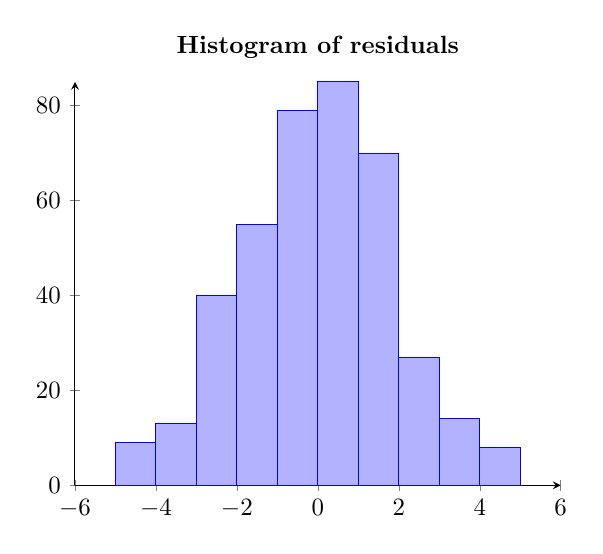
\begin{tikzpicture}[scale=0.9]
	\begin{axis}[
	ybar,
	ymin=0,
	axis y line=left,
	axis x line=bottom,
	domain=-6:-6,
	xmin=-6,
	xmax=6,
	title=\textbf{Histogram of residuals}
	]
	\addplot +[
	hist={
		bins=10,
		data min=-5,
		data max=5
	}   
	] table [y index=0] {
		dist
		-1.8970
		0.8230
		1.3540
		1.7155
		-1.3823
		0.8988
		0.2013
		1.6521
		1.0723
		1.7958
		-0.2639
		-0.2944
		2.0155
		-4.2473
		-1.0092
		-2.5412
		-0.7652
		1.2974
		1.6515
		-2.0299
		-0.9421
		0.2740
		-0.5837
		0.6036
		0.7999
		-1.8599
		-0.3537
		-4.2642
		2.2907
		-1.2582
		-2.4077
		-0.5079
		-2.8573
		-0.0417
		-1.1213
		4.3556
		2.2769
		-4.9938
		0.8827
		-2.7963
		-0.5101
		0.3288
		1.4955
		-0.5461
		3.1526
		-0.9619
		0.6550
		1.3295
		0.1704
		1.7619
		0.6464
		-1.5683
		-3.6107
		3.7172
		-1.2091
		0.2067
		1.1263
		0.2272
		-1.8095
		-0.9354
		-0.2498
		2.9579
		-1.7216
		1.5693
		0.6172
		-0.4677
		-2.1139
		-0.5683
		-0.1734
		-2.9388
		0.3844
		-1.6446
		-0.1885
		0.6724
		-1.8093
		-0.5765
		0.7001
		-3.6717
		2.0720
		4.8489
		1.9188
		-0.6315
		0.8572
		-2.0720
		3.7557
		1.8814
		1.5747
		-1.7517
		0.6399
		-1.1166
		-0.6229
		-1.1400
		-2.0515
		-1.8175
		-0.4198
		-3.3977
		1.2152
		-0.2356
		1.3983
		0.5393
		0.9886
		-2.9662
		-2.0405
		-0.8940
		0.2193
		2.2575
		-0.5799
		2.5231
		0.9508
		2.3482
		0.2539
		-1.3136
		-2.9628
		0.3110
		1.6371
		-0.5852
		-1.0816
		-0.6173
		-2.1932
		-0.9860
		-0.3615
		0.0917
		-0.1276
		1.2227
		0.2186
		3.6280
		0.6240
		3.6090
		-1.4462
		1.0531
		-0.5205
		1.2003
		1.1879
		-4.3720
		-2.6541
		-2.8820
		0.8037
		2.9404
		-0.6536
		1.6246
		1.0911
		-2.1033
		0.7949
		-1.5038
		3.0325
		-0.0651
		3.2720
		-0.8501
		1.1789
		-0.1256
		-4.0439
		-1.9643
		1.2250
		-0.1098
		-2.2375
		-1.2528
		0.4990
		-1.9860
		1.9499
		-1.2814
		3.6177
		-2.1597
		0.3984
		-3.0421
		-1.4473
		-1.1865
		0.8027
		1.8843
		0.6010
		-0.7461
		1.6310
		1.5978
		0.2404
		1.1425
		0.8256
		-1.9739
		1.5191
		-1.3144
		-1.2078
		0.3539
		-0.6150
		-0.2636
		1.1907
		2.0937
		-0.3959
		0.6554
		-0.4766
		0.4592
		0.8800
		-1.2337
		0.5497
		1.2022
		0.1846
		3.4597
		-1.2171
		-1.4741
		-3.4998
		1.8210
		1.7342
		-0.1598
		1.7970
		0.3674
		0.5816
		0.2259
		0.8799
		0.2033
		5.5747
		-2.3333
		-3.7086
		-2.2814
		-2.1867
		-0.8672
		-0.3369
		-0.4371
		1.0827
		0.7785
		1.5025
		3.5565
		2.4461
		-2.5665
		-4.6579
		1.8039
		-3.6713
		0.1335
		0.0710
		4.4543
		-0.1384
		-1.0146
		0.4716
		0.4916
		0.1401
		-1.2172
		-2.4452
		0.6330
		-2.6857
		-2.0644
		2.6624
		-0.8378
		-0.2806
		1.7996
		-0.6002
		2.0587
		-0.6901
		2.0256
		1.2587
		-0.4260
		-1.7314
		-2.0862
		-0.5401
		-0.8763
		-0.8173
		1.9671
		-0.5954
		2.2874
		-1.0632
		1.9451
		-1.0445
		0.3532
		1.9415
		-0.8279
		-0.8765
		4.0068
		1.9020
		-0.8640
		1.2979
		-0.7202
		1.4118
		2.8317
		-3.2090
		2.0577
		2.9159
		0.0949
		3.4925
		0.3108
		-2.4742
		-4.3870
		-0.6668
		1.4271
		0.6348
		0.8272
		-1.1542
		0.2880
		-3.2773
		-1.5202
		-1.6376
		1.0395
		-0.0283
		-2.3111
		-0.0190
		-1.3796
		-1.3334
		1.7283
		0.2268
		0.7967
		1.7679
		0.3605
		1.1017
		1.3659
		2.3412
		0.9517
		2.8245
		0.0452
		-0.0957
		3.4027
		-1.0194
		-0.0057
		1.8397
		0.2996
		2.8099
		2.0682
		0.5831
		-1.5554
		1.1334
		-2.7652
		0.4889
		1.6169
		0.4261
		1.7594
		4.0778
		1.8479
		0.5338
		1.2833
		0.8510
		-2.6294
		-0.8328
		2.4494
		-0.0872
		1.1648
		-2.0130
		0.1290
		1.2006
		-2.7230
		0.6952
		-0.3637
		-1.8791
		-0.0751
		-3.7926
		-4.2560
		-2.3538
		-1.9811
		-2.3461
		-3.4509
		0.5765
		-3.1884
		0.2204
		1.5741
		-0.0045
		0.1862
		-0.7563
		-2.9654
		-0.0876
		1.9217
		3.4765
		-0.8604
		-3.2546
		0.3327
		0.7525
		-0.4539
		-2.2978
		4.0487
		-4.7190
		-1.0199
		-2.6433
		-1.2723
		0.6357
		0.2761
		-1.4215
		1.5540
		1.2448
		1.2948
		-0.8513
		2.0972
		1.3214
		5.0175
		2.1269
		2.3138
		0.1060
		-2.5768
		-0.7424
		-1.5156
		-1.1279
		1.1103
		-1.1136
		-1.7902
		-0.8187
		-0.3218
		0.8187
		-1.9053
		0.6346
		0.1560
		2.6488
		-0.4263
		-0.2690
		-2.3427
		-2.7705
		0.6210
		-0.4990
		1.0075
		-1.7853
		3.8170
	};
	\end{axis}
	\end{tikzpicture}
	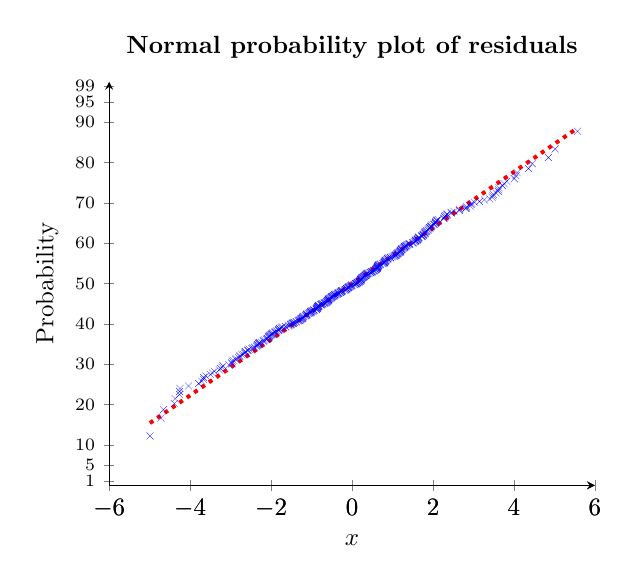
\begin{tikzpicture}[scale=0.9]
	\begin{axis}[
	xmin=-6, xmax=6, xlabel=$x$,
	ymin=-4, ymax=4, ylabel=$y$,
	samples=400,
	axis x line=bottom,
	axis y line=none,
	domain=-6:-6,
	title=\textbf{Normal probability plot of residuals}
	]
	\addplot[mark=x,blue, only marks, ultra thin] coordinates {
		(-4.99,-3.02)
		(-4.72,-2.67)
		(-4.66,-2.50)
		(-4.39,-2.38)
		(-4.37,-2.28)
		(-4.26,-2.20)
		(-4.26,-2.14)
		(-4.25,-2.08)
		(-4.04,-2.03)
		(-3.79,-1.98)
		(-3.71,-1.94)
		(-3.67,-1.90)
		(-3.67,-1.86)
		(-3.61,-1.83)
		(-3.50,-1.80)
		(-3.45,-1.77)
		(-3.40,-1.74)
		(-3.28,-1.71)
		(-3.25,-1.68)
		(-3.21,-1.66)
		(-3.19,-1.63)
		(-3.04,-1.61)
		(-2.97,-1.59)
		(-2.97,-1.57)
		(-2.96,-1.54)
		(-2.94,-1.52)
		(-2.88,-1.50)
		(-2.86,-1.49)
		(-2.80,-1.47)
		(-2.77,-1.45)
		(-2.77,-1.43)
		(-2.72,-1.41)
		(-2.69,-1.40)
		(-2.65,-1.38)
		(-2.64,-1.36)
		(-2.63,-1.35)
		(-2.58,-1.33)
		(-2.57,-1.32)
		(-2.54,-1.30)
		(-2.47,-1.29)
		(-2.45,-1.27)
		(-2.41,-1.26)
		(-2.35,-1.25)
		(-2.35,-1.23)
		(-2.34,-1.22)
		(-2.33,-1.21)
		(-2.31,-1.19)
		(-2.30,-1.18)
		(-2.28,-1.17)
		(-2.24,-1.16)
		(-2.19,-1.14)
		(-2.19,-1.13)
		(-2.16,-1.12)
		(-2.11,-1.11)
		(-2.10,-1.10)
		(-2.09,-1.09)
		(-2.07,-1.07)
		(-2.06,-1.06)
		(-2.05,-1.05)
		(-2.04,-1.04)
		(-2.03,-1.03)
		(-2.01,-1.02)
		(-1.99,-1.01)
		(-1.98,-1.00)
		(-1.97,-0.99)
		(-1.96,-0.98)
		(-1.91,-0.97)
		(-1.90,-0.96)
		(-1.88,-0.95)
		(-1.86,-0.94)
		(-1.82,-0.93)
		(-1.81,-0.92)
		(-1.81,-0.91)
		(-1.79,-0.90)
		(-1.79,-0.89)
		(-1.75,-0.88)
		(-1.73,-0.87)
		(-1.72,-0.86)
		(-1.64,-0.86)
		(-1.64,-0.85)
		(-1.57,-0.84)
		(-1.56,-0.83)
		(-1.52,-0.82)
		(-1.52,-0.81)
		(-1.50,-0.80)
		(-1.47,-0.79)
		(-1.45,-0.78)
		(-1.45,-0.78)
		(-1.42,-0.77)
		(-1.38,-0.76)
		(-1.38,-0.75)
		(-1.33,-0.74)
		(-1.31,-0.73)
		(-1.31,-0.73)
		(-1.28,-0.72)
		(-1.27,-0.71)
		(-1.26,-0.70)
		(-1.25,-0.69)
		(-1.23,-0.69)
		(-1.22,-0.68)
		(-1.22,-0.67)
		(-1.21,-0.66)
		(-1.21,-0.65)
		(-1.19,-0.65)
		(-1.15,-0.64)
		(-1.14,-0.63)
		(-1.13,-0.62)
		(-1.12,-0.62)
		(-1.12,-0.61)
		(-1.11,-0.60)
		(-1.08,-0.59)
		(-1.06,-0.59)
		(-1.04,-0.58)
		(-1.02,-0.57)
		(-1.02,-0.56)
		(-1.01,-0.56)
		(-1.01,-0.55)
		(-0.99,-0.54)
		(-0.96,-0.54)
		(-0.94,-0.53)
		(-0.94,-0.52)
		(-0.89,-0.51)
		(-0.88,-0.51)
		(-0.88,-0.50)
		(-0.87,-0.49)
		(-0.86,-0.49)
		(-0.86,-0.48)
		(-0.85,-0.47)
		(-0.85,-0.46)
		(-0.84,-0.46)
		(-0.83,-0.45)
		(-0.83,-0.44)
		(-0.82,-0.44)
		(-0.82,-0.43)
		(-0.77,-0.42)
		(-0.76,-0.42)
		(-0.75,-0.41)
		(-0.74,-0.40)
		(-0.72,-0.40)
		(-0.69,-0.39)
		(-0.67,-0.38)
		(-0.65,-0.38)
		(-0.63,-0.37)
		(-0.62,-0.36)
		(-0.62,-0.36)
		(-0.62,-0.35)
		(-0.60,-0.34)
		(-0.60,-0.34)
		(-0.59,-0.33)
		(-0.58,-0.32)
		(-0.58,-0.32)
		(-0.58,-0.31)
		(-0.57,-0.30)
		(-0.55,-0.30)
		(-0.54,-0.29)
		(-0.52,-0.28)
		(-0.51,-0.28)
		(-0.51,-0.27)
		(-0.50,-0.26)
		(-0.48,-0.26)
		(-0.47,-0.25)
		(-0.45,-0.24)
		(-0.44,-0.24)
		(-0.43,-0.23)
		(-0.43,-0.22)
		(-0.42,-0.22)
		(-0.40,-0.21)
		(-0.36,-0.21)
		(-0.36,-0.20)
		(-0.35,-0.19)
		(-0.34,-0.19)
		(-0.32,-0.18)
		(-0.29,-0.17)
		(-0.28,-0.17)
		(-0.27,-0.16)
		(-0.26,-0.15)
		(-0.26,-0.15)
		(-0.25,-0.14)
		(-0.24,-0.14)
		(-0.19,-0.13)
		(-0.17,-0.12)
		(-0.16,-0.12)
		(-0.14,-0.11)
		(-0.13,-0.10)
		(-0.13,-0.10)
		(-0.11,-0.09)
		(-0.10,-0.08)
		(-0.09,-0.08)
		(-0.09,-0.07)
		(-0.08,-0.07)
		(-0.07,-0.06)
		(-0.04,-0.05)
		(-0.03,-0.05)
		(-0.02,-0.04)
		(-0.01,-0.03)
		(-0.00,-0.03)
		(0.05,-0.02)
		(0.07,-0.02)
		(0.09,-0.01)
		(0.09,-0.00)
		(0.11,0.00)
		(0.13,0.01)
		(0.13,0.02)
		(0.14,0.02)
		(0.16,0.03)
		(0.17,0.03)
		(0.18,0.04)
		(0.19,0.05)
		(0.20,0.05)
		(0.20,0.06)
		(0.21,0.07)
		(0.22,0.07)
		(0.22,0.08)
		(0.22,0.08)
		(0.23,0.09)
		(0.23,0.10)
		(0.23,0.10)
		(0.24,0.11)
		(0.25,0.12)
		(0.27,0.12)
		(0.28,0.13)
		(0.29,0.14)
		(0.30,0.14)
		(0.31,0.15)
		(0.31,0.15)
		(0.33,0.16)
		(0.33,0.17)
		(0.35,0.17)
		(0.35,0.18)
		(0.36,0.19)
		(0.37,0.19)
		(0.38,0.20)
		(0.40,0.21)
		(0.43,0.21)
		(0.46,0.22)
		(0.47,0.22)
		(0.49,0.23)
		(0.49,0.24)
		(0.50,0.24)
		(0.53,0.25)
		(0.54,0.26)
		(0.55,0.26)
		(0.58,0.27)
		(0.58,0.28)
		(0.58,0.28)
		(0.60,0.29)
		(0.60,0.30)
		(0.62,0.30)
		(0.62,0.31)
		(0.62,0.32)
		(0.63,0.32)
		(0.63,0.33)
		(0.63,0.34)
		(0.64,0.34)
		(0.64,0.35)
		(0.65,0.36)
		(0.66,0.36)
		(0.66,0.37)
		(0.67,0.38)
		(0.70,0.38)
		(0.70,0.39)
		(0.75,0.40)
		(0.78,0.40)
		(0.79,0.41)
		(0.80,0.42)
		(0.80,0.42)
		(0.80,0.43)
		(0.80,0.44)
		(0.82,0.44)
		(0.82,0.45)
		(0.83,0.46)
		(0.83,0.46)
		(0.85,0.47)
		(0.86,0.48)
		(0.88,0.49)
		(0.88,0.49)
		(0.88,0.50)
		(0.90,0.51)
		(0.95,0.51)
		(0.95,0.52)
		(0.99,0.53)
		(1.01,0.54)
		(1.04,0.54)
		(1.05,0.55)
		(1.07,0.56)
		(1.08,0.56)
		(1.09,0.57)
		(1.10,0.58)
		(1.11,0.59)
		(1.13,0.59)
		(1.13,0.60)
		(1.14,0.61)
		(1.16,0.62)
		(1.18,0.62)
		(1.19,0.63)
		(1.19,0.64)
		(1.20,0.65)
		(1.20,0.65)
		(1.20,0.66)
		(1.22,0.67)
		(1.22,0.68)
		(1.23,0.69)
		(1.24,0.69)
		(1.26,0.70)
		(1.28,0.71)
		(1.29,0.72)
		(1.30,0.73)
		(1.30,0.73)
		(1.32,0.74)
		(1.33,0.75)
		(1.35,0.76)
		(1.37,0.77)
		(1.40,0.78)
		(1.41,0.78)
		(1.43,0.79)
		(1.50,0.80)
		(1.50,0.81)
		(1.52,0.82)
		(1.55,0.83)
		(1.57,0.84)
		(1.57,0.85)
		(1.57,0.86)
		(1.60,0.86)
		(1.62,0.87)
		(1.62,0.88)
		(1.63,0.89)
		(1.64,0.90)
		(1.65,0.91)
		(1.65,0.92)
		(1.72,0.93)
		(1.73,0.94)
		(1.73,0.95)
		(1.76,0.96)
		(1.76,0.97)
		(1.77,0.98)
		(1.80,0.99)
		(1.80,1.00)
		(1.80,1.01)
		(1.80,1.02)
		(1.82,1.03)
		(1.84,1.04)
		(1.85,1.05)
		(1.88,1.06)
		(1.88,1.07)
		(1.90,1.09)
		(1.92,1.10)
		(1.92,1.11)
		(1.94,1.12)
		(1.95,1.13)
		(1.95,1.14)
		(1.97,1.16)
		(2.02,1.17)
		(2.03,1.18)
		(2.06,1.19)
		(2.06,1.21)
		(2.07,1.22)
		(2.07,1.23)
		(2.09,1.25)
		(2.10,1.26)
		(2.13,1.27)
		(2.26,1.29)
		(2.28,1.30)
		(2.29,1.32)
		(2.29,1.33)
		(2.31,1.35)
		(2.34,1.36)
		(2.35,1.38)
		(2.45,1.40)
		(2.45,1.41)
		(2.52,1.43)
		(2.65,1.45)
		(2.66,1.47)
		(2.81,1.49)
		(2.82,1.50)
		(2.83,1.52)
		(2.92,1.54)
		(2.94,1.57)
		(2.96,1.59)
		(3.03,1.61)
		(3.15,1.63)
		(3.27,1.66)
		(3.40,1.68)
		(3.46,1.71)
		(3.48,1.74)
		(3.49,1.77)
		(3.56,1.80)
		(3.61,1.83)
		(3.62,1.86)
		(3.63,1.90)
		(3.72,1.94)
		(3.76,1.98)
		(3.82,2.03)
		(4.01,2.08)
		(4.05,2.14)
		(4.08,2.20)
		(4.36,2.28)
		(4.45,2.38)
		(4.85,2.50)
		(5.02,2.67)
		(5.57,3.02)
	};
	\addplot[dotted,red,ultra thick] coordinates {
		(-4.9938,-2.7658)
		(5.5747,3.0865)
	};
	\end{axis}
	\begin{axis}[
	xmin=-6,
	xmax=6,
	ymin=0,
	ymax=100,
	ylabel=Probability,
	axis y line=left,
	axis x line=bottom,
	yticklabel style={font=\scriptsize},
	ytick={1,5,10,20,30,40,50,60,70,80,90,95,99},
	]
	\end{axis}
	\end{tikzpicture}
\end{center}
\begin{center}
	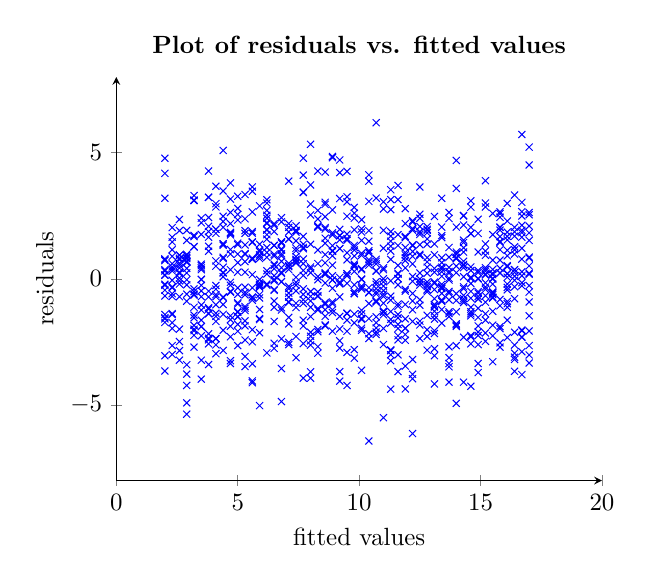
\begin{tikzpicture}[scale=0.9]
	\begin{axis}[
		xmin=0, xmax=20, xlabel=fitted values,
		ymin=-8, ymax=8, ylabel=residuals,
		samples=400,
		axis x line=bottom,
		axis y line=left,
		domain=0:20,
		title=\textbf{Plot of residuals vs. fitted values}
	]
		\addplot[mark=x,blue, only marks] coordinates {
			(2.00,-0.26)
			(2.00,-1.54)
			(2.00,4.78)
			(2.00,0.15)
			(2.00,0.75)
			(2.00,0.79)
			(2.00,-0.22)
			(2.00,-3.66)
			(2.00,4.18)
			(2.00,0.72)
			(2.00,-1.59)
			(2.00,-0.45)
			(2.00,3.19)
			(2.00,0.31)
			(2.00,0.36)
			(2.00,-0.68)
			(2.00,-3.05)
			(2.00,-1.42)
			(2.00,-1.73)
			(2.00,0.14)
			(2.30,0.31)
			(2.30,-0.36)
			(2.30,1.46)
			(2.30,-0.70)
			(2.30,0.47)
			(2.30,-1.74)
			(2.30,-1.97)
			(2.30,-0.59)
			(2.30,1.65)
			(2.30,0.39)
			(2.30,0.60)
			(2.30,-1.42)
			(2.30,-1.38)
			(2.30,1.15)
			(2.30,0.89)
			(2.30,-2.65)
			(2.30,-3.00)
			(2.30,2.03)
			(2.30,-0.06)
			(2.30,-0.32)
			(2.60,0.76)
			(2.60,-0.21)
			(2.60,0.43)
			(2.60,0.94)
			(2.60,-3.23)
			(2.60,0.03)
			(2.60,-0.08)
			(2.60,0.81)
			(2.60,0.61)
			(2.60,-2.49)
			(2.60,0.26)
			(2.60,-2.00)
			(2.60,-0.71)
			(2.60,0.21)
			(2.60,1.91)
			(2.60,0.93)
			(2.60,0.53)
			(2.60,-2.85)
			(2.60,0.22)
			(2.60,2.35)
			(2.90,-4.23)
			(2.90,0.92)
			(2.90,-4.92)
			(2.90,-0.61)
			(2.90,0.80)
			(2.90,-3.41)
			(2.90,1.52)
			(2.90,0.41)
			(2.90,1.92)
			(2.90,0.97)
			(2.90,-0.89)
			(2.90,0.65)
			(2.90,-0.04)
			(2.90,-3.78)
			(2.90,0.68)
			(2.90,0.68)
			(2.90,0.85)
			(2.90,0.23)
			(2.90,-0.24)
			(2.90,-5.37)
			(3.20,3.10)
			(3.20,-1.85)
			(3.20,-1.44)
			(3.20,1.67)
			(3.20,-1.13)
			(3.20,-2.00)
			(3.20,1.28)
			(3.20,-0.51)
			(3.20,-2.24)
			(3.20,3.30)
			(3.20,-0.61)
			(3.20,-1.55)
			(3.20,-2.71)
			(3.20,-0.65)
			(3.20,3.11)
			(3.20,1.26)
			(3.20,-2.06)
			(3.20,-0.40)
			(3.20,1.72)
			(3.20,3.12)
			(3.50,-0.26)
			(3.50,-1.64)
			(3.50,0.58)
			(3.50,-2.26)
			(3.50,1.76)
			(3.50,-1.89)
			(3.50,-1.24)
			(3.50,-3.98)
			(3.50,-1.90)
			(3.50,0.52)
			(3.50,2.40)
			(3.50,2.22)
			(3.50,-3.23)
			(3.50,-0.71)
			(3.50,-0.02)
			(3.50,-0.03)
			(3.50,0.43)
			(3.50,0.36)
			(3.50,-1.04)
			(3.50,-0.48)
			(3.80,-1.39)
			(3.80,-1.37)
			(3.80,1.87)
			(3.80,-2.42)
			(3.80,-0.72)
			(3.80,-2.36)
			(3.80,1.29)
			(3.80,-2.18)
			(3.80,-3.40)
			(3.80,-2.58)
			(3.80,1.09)
			(3.80,4.27)
			(3.80,-1.15)
			(3.80,1.65)
			(3.80,3.23)
			(3.80,2.43)
			(3.80,3.23)
			(3.80,-1.20)
			(3.80,2.08)
			(3.80,-0.49)
			(4.10,-2.97)
			(4.10,-0.71)
			(4.10,0.71)
			(4.10,3.67)
			(4.10,1.80)
			(4.10,0.50)
			(4.10,1.97)
			(4.10,-1.03)
			(4.10,-2.62)
			(4.10,-1.37)
			(4.10,-2.37)
			(4.10,1.96)
			(4.10,-0.27)
			(4.10,-2.38)
			(4.10,-0.41)
			(4.10,-1.69)
			(4.10,-0.63)
			(4.10,2.85)
			(4.10,2.98)
			(4.10,-1.49)
			(4.40,-0.75)
			(4.40,0.85)
			(4.40,0.23)
			(4.40,-1.02)
			(4.40,2.04)
			(4.40,-2.84)
			(4.40,5.09)
			(4.40,-0.72)
			(4.40,0.80)
			(4.40,-1.41)
			(4.40,-2.04)
			(4.40,2.27)
			(4.40,0.08)
			(4.40,0.46)
			(4.40,0.25)
			(4.40,1.39)
			(4.40,3.48)
			(4.40,1.33)
			(4.40,1.38)
			(4.40,2.48)
			(4.70,1.80)
			(4.70,-2.30)
			(4.70,-0.53)
			(4.70,-3.25)
			(4.70,1.16)
			(4.70,3.80)
			(4.70,3.16)
			(4.70,1.84)
			(4.70,-1.88)
			(4.70,-1.47)
			(4.70,0.36)
			(4.70,-0.26)
			(4.70,1.74)
			(4.70,2.63)
			(4.70,-0.50)
			(4.70,-0.14)
			(4.70,2.19)
			(4.70,0.98)
			(4.70,-3.36)
			(4.70,-1.62)
			(5.00,-1.50)
			(5.00,-2.65)
			(5.00,-0.36)
			(5.00,0.26)
			(5.00,2.79)
			(5.00,1.41)
			(5.00,2.33)
			(5.00,-1.51)
			(5.00,0.64)
			(5.00,3.27)
			(5.00,-1.30)
			(5.00,1.35)
			(5.00,2.55)
			(5.00,-2.08)
			(5.00,0.98)
			(5.00,-1.81)
			(5.00,-0.95)
			(5.00,-1.33)
			(5.00,-1.00)
			(5.00,-0.62)
			(5.30,-1.67)
			(5.30,-1.26)
			(5.30,1.00)
			(5.30,3.34)
			(5.30,-3.08)
			(5.30,-0.54)
			(5.30,0.68)
			(5.30,0.97)
			(5.30,1.91)
			(5.30,0.26)
			(5.30,-3.48)
			(5.30,1.34)
			(5.30,1.80)
			(5.30,-1.10)
			(5.30,-0.64)
			(5.30,-1.17)
			(5.30,-0.33)
			(5.30,-1.87)
			(5.30,2.38)
			(5.30,-2.43)
			(5.60,-0.76)
			(5.60,2.65)
			(5.60,0.77)
			(5.60,-0.72)
			(5.60,-0.85)
			(5.60,0.77)
			(5.60,1.81)
			(5.60,1.44)
			(5.60,3.47)
			(5.60,-2.02)
			(5.60,-0.36)
			(5.60,-4.05)
			(5.60,0.82)
			(5.60,1.47)
			(5.60,0.16)
			(5.60,-3.37)
			(5.60,-4.12)
			(5.60,3.64)
			(5.60,-2.50)
			(5.60,1.87)
			(5.90,-0.34)
			(5.90,-0.16)
			(5.90,-1.22)
			(5.90,1.14)
			(5.90,-0.31)
			(5.90,-2.14)
			(5.90,-0.63)
			(5.90,-0.03)
			(5.90,-0.26)
			(5.90,0.89)
			(5.90,0.80)
			(5.90,-5.03)
			(5.90,-1.58)
			(5.90,-0.23)
			(5.90,0.95)
			(5.90,1.37)
			(5.90,1.08)
			(5.90,-0.76)
			(5.90,2.89)
			(5.90,-1.62)
			(6.20,-2.94)
			(6.20,0.85)
			(6.20,1.93)
			(6.20,1.94)
			(6.20,1.04)
			(6.20,1.75)
			(6.20,0.32)
			(6.20,3.13)
			(6.20,2.71)
			(6.20,0.19)
			(6.20,1.57)
			(6.20,2.22)
			(6.20,3.00)
			(6.20,-0.26)
			(6.20,2.52)
			(6.20,2.19)
			(6.20,1.95)
			(6.20,2.40)
			(6.20,-0.21)
			(6.20,1.24)
			(6.50,2.18)
			(6.50,-0.88)
			(6.50,-2.56)
			(6.50,1.32)
			(6.50,0.40)
			(6.50,0.90)
			(6.50,-0.03)
			(6.50,-1.69)
			(6.50,0.97)
			(6.50,1.87)
			(6.50,0.58)
			(6.50,-0.43)
			(6.50,-0.08)
			(6.50,-0.46)
			(6.50,-2.76)
			(6.50,0.53)
			(6.50,2.12)
			(6.50,0.12)
			(6.50,-1.13)
			(6.50,1.33)
			(6.80,2.42)
			(6.80,0.91)
			(6.80,0.99)
			(6.80,0.44)
			(6.80,-1.15)
			(6.80,0.26)
			(6.80,2.26)
			(6.80,-0.11)
			(6.80,1.41)
			(6.80,-0.12)
			(6.80,1.18)
			(6.80,-1.24)
			(6.80,-2.38)
			(6.80,-4.87)
			(6.80,1.46)
			(6.80,0.69)
			(6.80,1.46)
			(6.80,1.14)
			(6.80,-3.56)
			(6.80,0.21)
			(7.10,3.87)
			(7.10,1.86)
			(7.10,-0.30)
			(7.10,-0.94)
			(7.10,-0.73)
			(7.10,0.52)
			(7.10,0.37)
			(7.10,-1.79)
			(7.10,-0.91)
			(7.10,-0.57)
			(7.10,2.19)
			(7.10,2.04)
			(7.10,0.61)
			(7.10,-2.52)
			(7.10,0.48)
			(7.10,1.57)
			(7.10,-0.39)
			(7.10,-2.61)
			(7.10,-1.53)
			(7.10,1.57)
			(7.40,-0.14)
			(7.40,0.77)
			(7.40,0.62)
			(7.40,1.50)
			(7.40,1.91)
			(7.40,0.88)
			(7.40,1.11)
			(7.40,0.73)
			(7.40,-2.29)
			(7.40,1.85)
			(7.40,2.10)
			(7.40,0.66)
			(7.40,-0.48)
			(7.40,-1.14)
			(7.40,-3.13)
			(7.40,0.06)
			(7.40,1.21)
			(7.40,1.92)
			(7.40,-0.25)
			(7.40,-0.97)
			(7.70,3.44)
			(7.70,3.42)
			(7.70,4.78)
			(7.70,-1.87)
			(7.70,-2.57)
			(7.70,0.33)
			(7.70,0.78)
			(7.70,1.37)
			(7.70,-0.98)
			(7.70,-0.40)
			(7.70,-0.62)
			(7.70,-3.94)
			(7.70,-1.64)
			(7.70,0.13)
			(7.70,-0.83)
			(7.70,1.68)
			(7.70,1.19)
			(7.70,0.60)
			(7.70,1.24)
			(7.70,4.11)
			(8.00,-0.50)
			(8.00,5.33)
			(8.00,3.72)
			(8.00,2.53)
			(8.00,-3.94)
			(8.00,-1.13)
			(8.00,-2.63)
			(8.00,0.40)
			(8.00,-2.12)
			(8.00,-0.88)
			(8.00,2.96)
			(8.00,-2.46)
			(8.00,-3.69)
			(8.00,-1.50)
			(8.00,-0.51)
			(8.00,1.37)
			(8.00,0.24)
			(8.00,-0.70)
			(8.00,0.47)
			(8.00,-2.28)
			(8.30,0.60)
			(8.30,2.07)
			(8.30,-0.04)
			(8.30,2.37)
			(8.30,-0.67)
			(8.30,2.04)
			(8.30,-2.69)
			(8.30,0.09)
			(8.30,1.14)
			(8.30,-2.10)
			(8.30,-2.95)
			(8.30,-1.18)
			(8.30,-0.52)
			(8.30,2.71)
			(8.30,-2.01)
			(8.30,2.09)
			(8.30,-0.52)
			(8.30,-1.24)
			(8.30,-0.70)
			(8.30,4.27)
			(8.60,-1.23)
			(8.60,3.03)
			(8.60,0.17)
			(8.60,-1.01)
			(8.60,1.41)
			(8.60,0.24)
			(8.60,-0.17)
			(8.60,0.96)
			(8.60,-0.95)
			(8.60,4.23)
			(8.60,0.20)
			(8.60,1.61)
			(8.60,2.03)
			(8.60,-1.87)
			(8.60,2.95)
			(8.60,1.97)
			(8.60,-1.49)
			(8.60,0.63)
			(8.60,-1.83)
			(8.60,2.46)
			(8.90,-0.05)
			(8.90,1.82)
			(8.90,0.12)
			(8.90,0.54)
			(8.90,-0.99)
			(8.90,-0.92)
			(8.90,-0.38)
			(8.90,4.85)
			(8.90,1.74)
			(8.90,1.12)
			(8.90,1.10)
			(8.90,4.80)
			(8.90,0.91)
			(8.90,1.31)
			(8.90,-1.23)
			(8.90,-0.04)
			(8.90,-2.08)
			(8.90,1.09)
			(8.90,-1.34)
			(8.90,2.73)
			(9.20,1.96)
			(9.20,-0.13)
			(9.20,-0.72)
			(9.20,-2.75)
			(9.20,1.70)
			(9.20,1.72)
			(9.20,-0.20)
			(9.20,4.21)
			(9.20,1.19)
			(9.20,1.20)
			(9.20,0.05)
			(9.20,1.54)
			(9.20,-1.49)
			(9.20,-0.19)
			(9.20,-1.99)
			(9.20,-2.46)
			(9.20,-3.68)
			(9.20,3.18)
			(9.20,-4.06)
			(9.20,4.71)
			(9.50,1.53)
			(9.50,-4.23)
			(9.50,-0.18)
			(9.50,1.77)
			(9.50,-1.38)
			(9.50,1.59)
			(9.50,-2.08)
			(9.50,0.20)
			(9.50,3.05)
			(9.50,0.75)
			(9.50,2.48)
			(9.50,0.13)
			(9.50,-1.36)
			(9.50,1.03)
			(9.50,0.11)
			(9.50,4.26)
			(9.50,-1.64)
			(9.50,0.20)
			(9.50,-2.92)
			(9.50,3.25)
			(9.80,1.32)
			(9.80,2.83)
			(9.80,-0.51)
			(9.80,0.90)
			(9.80,2.60)
			(9.80,-0.59)
			(9.80,1.14)
			(9.80,-2.81)
			(9.80,-0.59)
			(9.80,-0.24)
			(9.80,-1.40)
			(9.80,-3.15)
			(9.80,0.58)
			(9.80,0.48)
			(9.80,1.24)
			(9.80,1.94)
			(9.80,-1.75)
			(9.80,0.52)
			(9.80,0.29)
			(9.80,2.40)
			(10.10,1.85)
			(10.10,-1.57)
			(10.10,-3.63)
			(10.10,-1.62)
			(10.10,1.98)
			(10.10,-0.01)
			(10.10,-0.41)
			(10.10,-1.39)
			(10.10,-1.25)
			(10.10,0.93)
			(10.10,1.52)
			(10.10,1.01)
			(10.10,0.36)
			(10.10,2.34)
			(10.10,-0.36)
			(10.10,-0.03)
			(10.10,-1.96)
			(10.10,0.40)
			(10.10,-0.29)
			(10.10,-2.04)
			(10.40,1.11)
			(10.40,0.54)
			(10.40,4.12)
			(10.40,1.03)
			(10.40,1.04)
			(10.40,-0.35)
			(10.40,-2.18)
			(10.40,-2.37)
			(10.40,0.68)
			(10.40,3.07)
			(10.40,0.76)
			(10.40,1.91)
			(10.40,-0.98)
			(10.40,0.63)
			(10.40,-0.53)
			(10.40,-1.58)
			(10.40,1.49)
			(10.40,-0.56)
			(10.40,-6.43)
			(10.40,3.87)
			(10.70,-0.60)
			(10.70,0.77)
			(10.70,-0.91)
			(10.70,0.31)
			(10.70,-0.52)
			(10.70,-0.12)
			(10.70,-0.87)
			(10.70,-2.21)
			(10.70,-0.92)
			(10.70,0.59)
			(10.70,-0.39)
			(10.70,3.20)
			(10.70,6.19)
			(10.70,-1.51)
			(10.70,-1.74)
			(10.70,-2.11)
			(10.70,-1.95)
			(10.70,-0.22)
			(10.70,0.69)
			(10.70,0.31)
			(11.00,-2.61)
			(11.00,3.05)
			(11.00,1.92)
			(11.00,-1.97)
			(11.00,-0.47)
			(11.00,-0.97)
			(11.00,-0.12)
			(11.00,-1.28)
			(11.00,-1.43)
			(11.00,0.36)
			(11.00,-0.61)
			(11.00,-0.00)
			(11.00,-0.70)
			(11.00,-0.29)
			(11.00,0.43)
			(11.00,-1.31)
			(11.00,2.77)
			(11.00,1.21)
			(11.00,-5.51)
			(11.00,-1.33)
			(11.30,1.29)
			(11.30,1.87)
			(11.30,-2.85)
			(11.30,3.53)
			(11.30,-0.08)
			(11.30,-3.01)
			(11.30,-0.85)
			(11.30,-1.30)
			(11.30,3.14)
			(11.30,-4.38)
			(11.30,-1.61)
			(11.30,0.77)
			(11.30,1.49)
			(11.30,-3.25)
			(11.30,2.74)
			(11.30,-2.82)
			(11.30,-1.76)
			(11.30,-0.69)
			(11.30,1.69)
			(11.30,1.10)
			(11.60,0.01)
			(11.60,1.75)
			(11.60,-1.09)
			(11.60,3.14)
			(11.60,0.18)
			(11.60,-3.68)
			(11.60,-1.81)
			(11.60,-1.97)
			(11.60,-2.26)
			(11.60,1.32)
			(11.60,-2.42)
			(11.60,-0.00)
			(11.60,-0.24)
			(11.60,-1.55)
			(11.60,0.22)
			(11.60,-1.41)
			(11.60,3.70)
			(11.60,-3.02)
			(11.60,0.53)
			(11.60,-1.00)
			(11.90,-0.42)
			(11.90,-3.46)
			(11.90,1.68)
			(11.90,0.43)
			(11.90,2.19)
			(11.90,1.24)
			(11.90,-1.59)
			(11.90,-2.44)
			(11.90,-1.02)
			(11.90,1.04)
			(11.90,-2.21)
			(11.90,-0.49)
			(11.90,-4.37)
			(11.90,-1.97)
			(11.90,0.95)
			(11.90,1.63)
			(11.90,2.78)
			(11.90,0.84)
			(11.90,0.72)
			(11.90,-1.96)
			(12.20,-3.96)
			(12.20,1.99)
			(12.20,1.08)
			(12.20,0.89)
			(12.20,1.31)
			(12.20,-0.88)
			(12.20,2.25)
			(12.20,1.92)
			(12.20,-0.58)
			(12.20,-1.23)
			(12.20,-0.10)
			(12.20,1.34)
			(12.20,2.30)
			(12.20,1.98)
			(12.20,-3.79)
			(12.20,0.59)
			(12.20,-6.14)
			(12.20,-3.20)
			(12.20,-1.69)
			(12.20,0.09)
			(12.50,-0.12)
			(12.50,-0.25)
			(12.50,2.07)
			(12.50,0.23)
			(12.50,1.76)
			(12.50,-0.15)
			(12.50,-1.83)
			(12.50,-2.37)
			(12.50,2.40)
			(12.50,-0.83)
			(12.50,0.97)
			(12.50,-0.01)
			(12.50,-1.05)
			(12.50,0.92)
			(12.50,-1.68)
			(12.50,1.84)
			(12.50,2.56)
			(12.50,3.64)
			(12.50,1.35)
			(12.50,1.87)
			(12.80,1.58)
			(12.80,-2.02)
			(12.80,-0.23)
			(12.80,0.84)
			(12.80,-2.29)
			(12.80,-0.45)
			(12.80,-2.83)
			(12.80,-0.52)
			(12.80,0.46)
			(12.80,0.67)
			(12.80,1.37)
			(12.80,1.96)
			(12.80,-0.43)
			(12.80,1.92)
			(12.80,2.07)
			(12.80,-0.31)
			(12.80,0.22)
			(12.80,1.82)
			(12.80,-0.13)
			(12.80,-1.45)
			(13.10,-1.02)
			(13.10,-1.29)
			(13.10,-2.17)
			(13.10,2.47)
			(13.10,-4.17)
			(13.10,-0.18)
			(13.10,0.26)
			(13.10,0.41)
			(13.10,-0.43)
			(13.10,-3.05)
			(13.10,-1.09)
			(13.10,-2.06)
			(13.10,1.38)
			(13.10,-0.79)
			(13.10,0.95)
			(13.10,-0.13)
			(13.10,-1.12)
			(13.10,-1.47)
			(13.10,-2.77)
			(13.10,-1.60)
			(13.40,-1.22)
			(13.40,-0.22)
			(13.40,0.83)
			(13.40,0.46)
			(13.40,1.71)
			(13.40,0.10)
			(13.40,2.05)
			(13.40,-0.36)
			(13.40,-0.58)
			(13.40,1.63)
			(13.40,0.64)
			(13.40,0.28)
			(13.40,-0.90)
			(13.40,-0.31)
			(13.40,-1.76)
			(13.40,-0.39)
			(13.40,0.39)
			(13.40,3.19)
			(13.40,-0.88)
			(13.40,-0.84)
			(13.70,0.45)
			(13.70,0.29)
			(13.70,0.02)
			(13.70,0.22)
			(13.70,-4.10)
			(13.70,2.63)
			(13.70,1.24)
			(13.70,-0.84)
			(13.70,-1.31)
			(13.70,-1.38)
			(13.70,-3.36)
			(13.70,-0.50)
			(13.70,2.39)
			(13.70,-3.13)
			(13.70,-3.49)
			(13.70,-0.05)
			(13.70,-2.70)
			(13.70,-0.57)
			(13.70,-1.50)
			(13.70,0.86)
			(14.00,-0.86)
			(14.00,0.24)
			(14.00,0.84)
			(14.00,0.81)
			(14.00,0.97)
			(14.00,-0.59)
			(14.00,-4.94)
			(14.00,0.50)
			(14.00,-1.86)
			(14.00,1.06)
			(14.00,-2.65)
			(14.00,2.05)
			(14.00,-1.80)
			(14.00,-1.31)
			(14.00,0.80)
			(14.00,4.69)
			(14.00,-1.89)
			(14.00,3.58)
			(14.00,0.98)
			(14.00,-1.79)
			(14.30,1.53)
			(14.30,0.44)
			(14.30,-0.94)
			(14.30,-0.87)
			(14.30,-4.10)
			(14.30,-0.32)
			(14.30,1.06)
			(14.30,0.53)
			(14.30,-0.66)
			(14.30,2.13)
			(14.30,-0.79)
			(14.30,1.23)
			(14.30,-2.32)
			(14.30,-0.39)
			(14.30,0.57)
			(14.30,1.44)
			(14.30,0.08)
			(14.30,0.69)
			(14.30,2.51)
			(14.30,2.49)
			(14.60,-1.13)
			(14.60,0.47)
			(14.60,3.09)
			(14.60,0.33)
			(14.60,0.06)
			(14.60,2.84)
			(14.60,1.78)
			(14.60,-1.31)
			(14.60,0.01)
			(14.60,-2.25)
			(14.60,-0.50)
			(14.60,1.80)
			(14.60,-2.58)
			(14.60,2.04)
			(14.60,-0.77)
			(14.60,-1.39)
			(14.60,-1.47)
			(14.60,-4.26)
			(14.60,-0.19)
			(14.60,-2.30)
			(14.90,-3.36)
			(14.90,-0.01)
			(14.90,-1.17)
			(14.90,-0.80)
			(14.90,0.25)
			(14.90,0.33)
			(14.90,-0.70)
			(14.90,-0.57)
			(14.90,-0.80)
			(14.90,-0.51)
			(14.90,-1.87)
			(14.90,-2.61)
			(14.90,-2.25)
			(14.90,1.06)
			(14.90,0.01)
			(14.90,1.80)
			(14.90,2.36)
			(14.90,-1.53)
			(14.90,-2.11)
			(14.90,-3.72)
			(15.20,-0.42)
			(15.20,1.38)
			(15.20,3.00)
			(15.20,0.15)
			(15.20,-0.93)
			(15.20,0.44)
			(15.20,-1.64)
			(15.20,0.18)
			(15.20,-0.16)
			(15.20,-2.48)
			(15.20,-0.67)
			(15.20,0.93)
			(15.20,2.85)
			(15.20,1.10)
			(15.20,3.89)
			(15.20,-1.39)
			(15.20,0.37)
			(15.20,-0.33)
			(15.20,0.30)
			(15.20,-2.15)
			(15.50,-0.21)
			(15.50,-0.63)
			(15.50,-0.75)
			(15.50,-0.73)
			(15.50,-0.52)
			(15.50,0.02)
			(15.50,2.59)
			(15.50,-0.76)
			(15.50,-0.01)
			(15.50,-3.29)
			(15.50,0.37)
			(15.50,0.16)
			(15.50,-1.29)
			(15.50,0.74)
			(15.50,-0.57)
			(15.50,-0.54)
			(15.50,-2.26)
			(15.50,1.75)
			(15.50,-1.84)
			(15.50,0.22)
			(15.80,0.24)
			(15.80,1.44)
			(15.80,1.48)
			(15.80,-2.71)
			(15.80,2.58)
			(15.80,1.15)
			(15.80,-1.90)
			(15.80,-1.98)
			(15.80,-0.82)
			(15.80,-1.07)
			(15.80,1.93)
			(15.80,2.04)
			(15.80,0.42)
			(15.80,2.05)
			(15.80,0.22)
			(15.80,2.65)
			(15.80,2.44)
			(15.80,-2.54)
			(15.80,1.67)
			(15.80,0.74)
			(16.10,-0.44)
			(16.10,1.68)
			(16.10,-0.90)
			(16.10,-1.13)
			(16.10,1.13)
			(16.10,-0.21)
			(16.10,0.19)
			(16.10,2.29)
			(16.10,-0.99)
			(16.10,0.48)
			(16.10,1.54)
			(16.10,-2.33)
			(16.10,0.21)
			(16.10,-0.34)
			(16.10,0.91)
			(16.10,0.52)
			(16.10,0.06)
			(16.10,-1.64)
			(16.10,1.85)
			(16.10,2.99)
			(16.40,0.98)
			(16.40,1.69)
			(16.40,0.10)
			(16.40,-0.79)
			(16.40,0.36)
			(16.40,-3.11)
			(16.40,3.32)
			(16.40,1.86)
			(16.40,-3.67)
			(16.40,-2.63)
			(16.40,1.15)
			(16.40,-0.32)
			(16.40,-0.06)
			(16.40,-3.20)
			(16.40,0.25)
			(16.40,0.36)
			(16.40,1.27)
			(16.40,-2.95)
			(16.40,2.04)
			(16.40,-2.12)
			(16.70,0.12)
			(16.70,3.03)
			(16.70,2.66)
			(16.70,0.78)
			(16.70,2.12)
			(16.70,-2.31)
			(16.70,1.65)
			(16.70,1.83)
			(16.70,-2.06)
			(16.70,0.28)
			(16.70,5.72)
			(16.70,1.92)
			(16.70,2.49)
			(16.70,1.21)
			(16.70,-2.32)
			(16.70,-3.80)
			(16.70,-0.16)
			(16.70,-2.03)
			(16.70,-2.89)
			(16.70,-0.28)
			(17.00,0.86)
			(17.00,4.51)
			(17.00,-0.92)
			(17.00,0.18)
			(17.00,5.22)
			(17.00,-2.07)
			(17.00,0.51)
			(17.00,-0.53)
			(17.00,2.63)
			(17.00,0.22)
			(17.00,2.54)
			(17.00,0.82)
			(17.00,1.52)
			(17.00,-3.34)
			(17.00,-1.47)
			(17.00,-2.65)
			(17.00,-3.02)
			(17.00,1.82)
			(17.00,2.09)
			(17.00,-0.27)
		};
	\end{axis}
	\end{tikzpicture}
	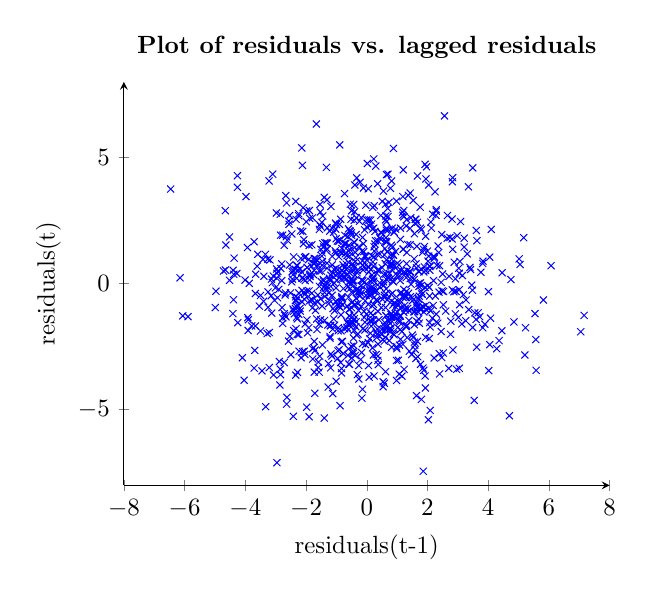
\begin{tikzpicture}[scale=0.9]
	\begin{axis}[
	xmin=-8, xmax=8, xlabel=residuals(t-1),
	ymin=-8, ymax=8, ylabel=residuals(t),
	samples=400,
	axis x line=bottom,
	axis y line=left,
	domain=-8:-8,
	title=\textbf{Plot of residuals vs. lagged residuals}
	]
	\addplot[mark=x,blue, only marks] coordinates {
		(3.67,-1.16)
		(-4.52,1.85)
		(1.72,0.01)
		(0.64,-1.27)
		(-2.62,1.72)
		(-0.87,-0.96)
		(0.69,2.98)
		(7.16,-1.26)
		(5.54,-1.19)
		(-2.70,-1.26)
		(6.07,0.71)
		(1.45,2.61)
		(-0.13,0.73)
		(1.43,1.54)
		(-0.41,2.51)
		(-0.25,-0.26)
		(2.98,1.90)
		(2.82,-0.25)
		(2.83,4.20)
		(1.34,0.52)
		(-2.41,-1.09)
		(1.43,0.20)
		(3.26,-1.47)
		(0.98,-3.05)
		(2.07,0.70)
		(1.45,0.47)
		(-0.61,1.31)
		(0.59,-1.69)
		(-1.57,-1.61)
		(1.78,-0.98)
		(-2.29,-2.01)
		(-2.14,5.38)
		(-1.62,0.74)
		(-5.89,-1.31)
		(2.88,0.85)
		(0.65,2.46)
		(-1.51,1.36)
		(2.74,1.83)
		(-3.42,0.96)
		(-0.20,-3.01)
		(-0.48,-1.52)
		(0.64,2.12)
		(0.63,-0.40)
		(-1.73,0.52)
		(-0.06,1.11)
		(-0.33,-2.04)
		(1.26,0.38)
		(2.19,-0.87)
		(2.22,-2.95)
		(-1.73,0.79)
		(0.15,-1.69)
		(-2.43,-1.01)
		(-2.23,-2.68)
		(-0.01,-1.21)
		(3.07,0.88)
		(-1.54,3.14)
		(0.74,-2.26)
		(-0.45,0.69)
		(2.23,1.05)
		(-2.18,2.09)
		(0.07,2.52)
		(1.11,-2.21)
		(2.20,0.12)
		(3.09,2.46)
		(0.17,1.09)
		(-2.98,2.80)
		(-1.48,2.43)
		(-2.12,4.69)
		(4.70,-5.24)
		(-1.23,-0.66)
		(1.50,-0.68)
		(-0.38,-2.85)
		(1.78,-1.04)
		(-1.53,2.84)
		(-2.80,0.12)
		(-2.84,1.92)
		(0.98,3.27)
		(-0.35,-0.58)
		(-0.39,-0.82)
		(2.84,-2.63)
		(0.58,-0.55)
		(0.40,-1.43)
		(3.18,-0.44)
		(-1.61,-0.45)
		(1.39,-1.46)
		(1.67,-2.29)
		(-0.49,-0.76)
		(0.43,0.03)
		(-2.33,-1.79)
		(-2.30,0.70)
		(0.21,-0.29)
		(1.44,-0.52)
		(5.17,1.82)
		(-1.33,4.61)
		(0.37,1.70)
		(-0.16,1.29)
		(-3.87,0.01)
		(-0.88,0.26)
		(-3.59,1.16)
		(1.68,-1.11)
		(-1.78,-2.99)
		(0.20,0.86)
		(-1.09,-1.40)
		(0.61,0.79)
		(-1.20,-1.66)
		(0.98,-2.51)
		(1.48,-2.81)
		(3.42,0.56)
		(-0.39,3.91)
		(-4.28,0.40)
		(-1.68,0.98)
		(2.71,0.29)
		(-2.14,0.46)
		(1.92,4.73)
		(0.25,-1.56)
		(2.87,-0.32)
		(-3.92,-1.35)
		(-0.40,1.43)
		(-2.42,0.51)
		(5.82,-0.65)
		(1.65,1.48)
		(2.76,-2.01)
		(-2.12,0.24)
		(-0.94,0.40)
		(-0.54,3.15)
		(2.20,1.08)
		(-0.56,0.07)
		(1.40,-2.68)
		(-4.10,-2.94)
		(-0.71,1.18)
		(-1.65,-1.40)
		(-3.15,-0.48)
		(1.02,-1.74)
		(0.56,0.36)
		(0.07,0.46)
		(-2.67,3.49)
		(2.25,3.64)
		(0.70,2.12)
		(-0.60,2.17)
		(0.05,-2.34)
		(-0.52,2.55)
		(-3.50,-1.88)
		(-0.57,-3.20)
		(-1.66,6.33)
		(-1.96,0.64)
		(-2.31,-1.33)
		(-1.07,0.02)
		(-4.01,0.14)
		(1.93,-4.14)
		(1.04,-1.43)
		(-0.04,1.06)
		(-0.07,0.07)
		(-1.60,-3.33)
		(2.04,-0.98)
		(-0.27,-0.30)
		(-1.43,0.16)
		(2.70,-3.36)
		(-0.45,0.51)
		(-1.18,3.06)
		(-0.59,-3.19)
		(-1.70,0.88)
		(-2.24,2.69)
		(5.05,0.76)
		(3.31,1.18)
		(0.62,-0.95)
		(-2.51,-0.37)
		(-1.73,-2.29)
		(-0.35,-0.24)
		(1.58,-1.11)
		(-2.66,-1.32)
		(-4.66,2.89)
		(-2.90,-0.23)
		(0.67,1.26)
		(0.78,0.75)
		(0.90,-2.03)
		(-0.26,-3.78)
		(0.37,-2.87)
		(-0.95,0.55)
		(1.72,-0.60)
		(-2.72,1.52)
		(0.91,-0.76)
		(-1.70,-2.64)
		(-0.67,0.19)
		(1.11,2.20)
		(2.08,0.53)
		(-2.24,-0.37)
		(2.52,-0.84)
		(1.32,2.54)
		(-0.14,1.83)
		(-0.39,-0.86)
		(-0.44,-2.69)
		(-0.61,-1.83)
		(0.05,0.67)
		(0.10,-2.19)
		(1.65,-0.77)
		(3.05,-0.24)
		(0.93,-1.32)
		(-0.42,-1.25)
		(1.25,-0.45)
		(0.37,-1.10)
		(-2.06,-2.68)
		(1.90,1.47)
		(0.61,-1.84)
		(0.27,2.07)
		(1.03,-0.69)
		(0.52,-0.62)
		(-1.88,2.59)
		(-0.32,0.52)
		(-0.29,-0.80)
		(-1.06,-1.65)
		(3.36,-1.03)
		(-1.75,0.80)
		(-0.97,1.69)
		(-1.42,0.10)
		(-2.35,-0.99)
		(-0.38,0.67)
		(-0.55,1.34)
		(3.06,-0.84)
		(-0.50,2.89)
		(-2.13,-0.73)
		(3.21,1.80)
		(2.47,1.94)
		(-0.46,0.11)
		(-3.01,-0.17)
		(-0.89,1.74)
		(-0.31,-3.61)
		(0.55,0.07)
		(-0.52,0.14)
		(0.89,0.73)
		(0.78,-1.77)
		(-2.50,-2.82)
		(-1.90,-5.28)
		(-1.48,1.09)
		(-1.02,2.16)
		(-0.64,-0.89)
		(0.02,4.76)
		(-6.06,-1.28)
		(-0.91,-2.62)
		(2.48,-0.29)
		(-2.13,0.21)
		(1.87,1.36)
		(0.70,0.24)
		(-0.06,-1.53)
		(0.36,-3.05)
		(-3.13,-1.17)
		(-0.17,-2.73)
		(3.21,1.45)
		(0.20,-0.21)
		(0.08,-3.71)
		(-1.47,0.73)
		(-0.06,-1.84)
		(0.46,2.70)
		(0.85,0.10)
		(-0.75,0.46)
		(-0.47,-1.57)
		(4.05,1.05)
		(-4.52,0.13)
		(4.46,0.43)
		(0.68,-0.64)
		(2.00,1.29)
		(-3.33,-4.88)
		(-1.18,0.33)
		(-0.56,2.10)
		(0.85,-0.38)
		(-3.34,1.16)
		(0.94,-1.19)
		(-2.43,0.35)
		(0.13,-1.17)
		(1.30,2.29)
		(0.65,0.94)
		(2.17,2.75)
		(2.01,-0.08)
		(-1.30,-0.12)
		(0.51,0.63)
		(-1.89,2.90)
		(-2.64,-4.78)
		(1.85,-3.35)
		(0.00,2.53)
		(-0.11,3.79)
		(1.82,-0.41)
		(1.19,2.71)
		(0.70,4.34)
		(2.50,0.38)
		(1.86,-0.91)
		(0.48,-0.95)
		(-1.38,-0.51)
		(-1.30,1.60)
		(2.38,-0.34)
		(-3.22,4.07)
		(-0.05,-0.68)
		(-3.90,-1.43)
		(2.04,1.09)
		(1.72,0.47)
		(0.00,0.93)
		(-0.14,-4.19)
		(-4.97,-0.30)
		(1.16,-3.67)
		(-4.38,0.37)
		(-4.64,1.53)
		(0.16,2.36)
		(-1.90,1.51)
		(0.82,0.97)
		(1.35,1.55)
		(1.72,-0.11)
		(-1.38,-0.08)
		(0.90,2.04)
		(0.20,2.17)
		(1.65,-0.94)
		(1.07,-3.59)
		(1.80,-4.59)
		(-0.26,-3.25)
		(-0.29,-2.00)
		(2.02,0.89)
		(-4.25,-1.55)
		(-1.01,-0.17)
		(-2.54,0.74)
		(-0.77,-2.77)
		(1.30,-1.70)
		(1.65,-1.50)
		(-2.03,-1.60)
		(-0.94,-0.88)
		(0.27,1.57)
		(-0.58,-1.01)
		(0.60,1.39)
		(0.80,0.68)
		(-1.86,0.38)
		(-0.35,1.95)
		(-4.26,4.28)
		(2.29,2.93)
		(-1.26,-3.17)
		(-2.41,1.06)
		(-0.51,-2.49)
		(-2.86,-4.02)
		(-0.04,-2.42)
		(-1.12,-4.36)
		(4.36,-2.26)
		(2.28,2.71)
		(-4.99,-0.95)
		(0.88,5.36)
		(-2.80,0.78)
		(-0.51,2.01)
		(0.33,-0.29)
		(1.50,-0.56)
		(-0.55,-1.57)
		(3.15,0.32)
		(-0.96,-2.97)
		(0.66,-1.70)
		(1.33,-2.14)
		(0.17,0.34)
		(1.76,3.03)
		(0.65,4.32)
		(-1.57,-3.51)
		(-3.61,0.69)
		(3.72,-1.31)
		(-1.21,-2.16)
		(0.21,0.21)
		(1.13,-0.94)
		(0.23,0.10)
		(-1.81,1.54)
		(-0.94,-1.87)
		(-0.25,-0.31)
		(2.96,-3.40)
		(-1.72,-0.77)
		(1.57,1.98)
		(0.62,-3.49)
		(-0.47,0.78)
		(-2.11,-2.70)
		(-0.57,0.44)
		(-0.17,-0.90)
		(-2.94,-0.56)
		(0.38,-3.21)
		(-1.64,-1.82)
		(-0.19,-0.39)
		(0.67,0.14)
		(-1.81,-0.38)
		(-0.58,-1.28)
		(0.70,2.66)
		(-3.67,-0.39)
		(2.07,-1.55)
		(4.85,-1.52)
		(1.92,-0.15)
		(-0.63,1.86)
		(0.86,-0.85)
		(-2.07,1.74)
		(3.76,0.45)
		(1.88,-1.13)
		(1.57,-1.63)
		(-1.75,0.35)
		(0.64,-0.21)
		(-1.12,-1.81)
		(-0.62,-1.59)
		(-1.14,1.08)
		(-2.05,1.04)
		(-1.82,-0.62)
		(-0.42,1.65)
		(-3.40,-0.70)
		(1.22,-0.23)
		(-0.24,2.47)
		(1.40,-1.08)
		(0.54,-4.09)
		(0.99,-2.58)
		(-2.97,0.58)
		(-2.04,-0.43)
		(-0.89,5.50)
		(0.22,-2.83)
		(2.26,-0.49)
		(-0.58,0.08)
		(2.52,-2.75)
		(0.95,2.16)
		(2.35,1.49)
		(0.25,3.09)
		(-1.31,1.38)
		(-2.96,-7.10)
		(0.31,-1.93)
		(1.64,0.62)
		(-0.59,-1.63)
		(-1.08,0.57)
		(-0.62,-0.13)
		(-2.19,-1.09)
		(-0.99,0.14)
		(-0.36,1.03)
		(0.09,2.29)
		(-0.13,-1.79)
		(1.22,-1.14)
		(0.22,-1.44)
		(3.63,1.70)
		(0.62,3.15)
		(3.61,2.11)
		(-1.45,2.68)
		(1.05,0.50)
		(-0.52,-1.60)
		(1.20,1.36)
		(1.19,3.45)
		(-4.37,1.01)
		(-2.65,1.86)
		(-2.88,-3.09)
		(0.80,1.14)
		(2.94,-0.31)
		(-0.65,1.11)
		(1.62,2.55)
		(1.09,-1.28)
		(-2.10,3.01)
		(0.79,-1.89)
		(-1.50,0.08)
		(3.03,0.61)
		(-0.07,2.13)
		(3.27,-0.65)
		(-0.85,-1.87)
		(1.18,2.83)
		(-0.13,0.73)
		(-4.04,-3.83)
		(-1.96,0.64)
		(1.23,-3.40)
		(-0.11,1.58)
		(-2.24,2.77)
		(-1.25,-0.37)
		(0.50,-1.82)
		(-1.99,2.45)
		(1.95,-1.02)
		(-1.28,-1.64)
		(3.62,-2.52)
		(-2.16,-2.94)
		(0.40,0.55)
		(-3.04,-0.66)
		(-1.45,1.58)
		(-1.19,-0.11)
		(0.80,-0.42)
		(1.88,-3.44)
		(0.60,-1.55)
		(-0.75,0.21)
		(1.63,-0.86)
		(1.60,2.55)
		(0.24,-3.66)
		(1.14,-0.36)
		(0.83,0.23)
		(-1.97,-1.44)
		(1.52,0.22)
		(-1.31,3.32)
		(-1.21,-2.10)
		(0.35,-0.70)
		(-0.62,-2.84)
		(-0.26,1.46)
		(1.19,-2.41)
		(2.09,-1.72)
		(-0.40,2.85)
		(0.66,1.65)
		(-0.48,-1.51)
		(0.46,2.03)
		(0.88,-1.32)
		(-1.23,0.21)
		(0.55,3.67)
		(1.20,4.51)
		(0.18,-0.89)
		(3.46,-0.06)
		(-1.22,2.08)
		(-1.47,1.22)
		(-3.50,-0.47)
		(1.82,-0.42)
		(1.73,-1.57)
		(-0.16,-4.54)
		(1.80,-0.31)
		(0.37,-2.40)
		(0.58,-0.46)
		(0.23,4.94)
		(0.88,0.07)
		(0.20,3.02)
		(5.57,-2.22)
		(-2.33,2.55)
		(-3.71,-3.35)
		(-2.28,-0.56)
		(-2.19,0.58)
		(-0.87,1.24)
		(-0.34,-0.25)
		(-0.44,-2.16)
		(1.08,-2.44)
		(0.78,-1.44)
		(1.50,-2.04)
		(3.56,-1.16)
		(2.45,-1.90)
		(-2.57,2.48)
		(-4.66,0.54)
		(1.80,0.57)
		(-3.67,-1.68)
		(0.13,0.55)
		(0.07,0.65)
		(4.45,-1.87)
		(-0.14,-2.38)
		(-1.01,-3.87)
		(0.47,1.75)
		(0.49,-2.02)
		(0.14,0.09)
		(-1.22,0.17)
		(-2.45,0.18)
		(0.63,-1.28)
		(-2.69,-0.45)
		(-2.06,-0.61)
		(2.66,2.70)
		(-0.84,-2.31)
		(-0.28,-0.41)
		(1.80,2.13)
		(-0.60,0.84)
		(2.06,-2.18)
		(-0.69,1.59)
		(2.03,-5.40)
		(1.26,-0.99)
		(-0.43,3.14)
		(-1.73,1.00)
		(-2.09,1.58)
		(-0.54,-0.19)
		(-0.88,-0.76)
		(-0.82,1.39)
		(1.97,4.63)
		(-0.60,-0.54)
		(2.29,2.87)
		(-1.06,-1.08)
		(1.95,-0.86)
		(-1.04,1.30)
		(0.35,-1.80)
		(1.94,1.88)
		(-0.83,-3.37)
		(-0.88,-4.84)
		(4.01,-0.32)
		(1.90,0.66)
		(-0.86,2.55)
		(1.30,0.24)
		(-0.72,1.91)
		(1.41,0.48)
		(2.83,1.36)
		(-3.21,-1.94)
		(2.06,-0.15)
		(2.92,-1.20)
		(0.09,-0.47)
		(3.49,4.59)
		(0.31,-2.81)
		(-2.47,0.07)
		(-4.39,-0.64)
		(-0.67,0.76)
		(1.43,3.59)
		(0.63,1.82)
		(0.83,-1.31)
		(-1.15,-2.87)
		(0.29,1.70)
		(-3.28,-1.98)
		(-1.52,-1.43)
		(-1.64,0.93)
		(1.04,-3.04)
		(-0.03,3.11)
		(-2.31,0.21)
		(-0.02,-0.47)
		(-1.38,1.62)
		(-1.33,1.61)
		(1.73,-0.50)
		(0.23,2.20)
		(0.80,0.73)
		(1.77,2.20)
		(0.36,0.53)
		(1.10,-0.38)
		(1.37,3.50)
		(2.34,-1.57)
		(0.95,1.27)
		(2.82,4.04)
		(0.05,-0.83)
		(-0.10,1.27)
		(3.40,0.64)
		(-1.02,-0.70)
		(-0.01,-0.01)
		(1.84,1.24)
		(0.30,4.66)
		(2.81,1.77)
		(2.07,-0.49)
		(0.58,-3.95)
		(-1.56,0.50)
		(1.13,0.52)
		(-2.77,-1.58)
		(0.49,2.02)
		(1.62,0.78)
		(0.43,1.17)
		(1.76,-0.97)
		(4.08,-1.37)
		(1.85,-0.93)
		(0.53,-2.22)
		(1.28,-1.05)
		(0.85,1.45)
		(-2.63,-4.51)
		(-0.83,-3.54)
		(2.45,0.05)
		(-0.09,0.66)
		(1.16,-1.90)
		(-2.01,1.07)
		(0.13,2.52)
		(1.20,1.37)
		(-2.72,-3.13)
		(0.70,-1.46)
		(-0.36,-1.71)
		(-1.88,-0.68)
		(-0.08,-1.34)
		(-3.79,-1.68)
		(-4.26,3.82)
		(-2.35,-0.67)
		(-1.98,-0.30)
		(-2.35,0.57)
		(-3.45,-3.46)
		(0.58,-2.28)
		(-3.19,0.94)
		(0.22,0.70)
		(1.57,-2.32)
		(-0.00,2.25)
		(0.19,-0.13)
		(-0.76,0.28)
		(-2.97,0.22)
		(-0.09,-1.10)
		(1.92,-3.66)
		(3.48,-0.26)
		(-0.86,-3.13)
		(-3.25,-0.33)
		(0.33,0.41)
		(0.75,0.40)
		(-0.45,-2.77)
		(-2.30,0.73)
		(4.05,-2.42)
		(-4.72,0.50)
		(-1.02,1.21)
		(-2.64,3.20)
		(-1.27,-4.10)
		(0.64,1.66)
		(0.28,-0.32)
		(-1.42,-0.15)
		(1.55,-1.12)
		(1.24,0.47)
		(1.29,-0.52)
		(-0.85,-1.24)
		(2.10,-1.08)
		(1.32,1.23)
		(5.02,0.98)
		(2.13,2.20)
		(2.31,0.73)
		(0.11,-0.29)
		(-2.58,-2.28)
		(-0.74,0.63)
		(-1.52,-0.61)
		(-1.13,0.44)
		(1.11,1.75)
		(-1.11,-0.99)
		(-1.79,-0.96)
		(-0.82,-0.52)
		(-0.32,0.43)
		(0.82,4.07)
		(-1.91,-1.75)
		(0.63,2.68)
		(0.16,-0.43)
		(2.65,1.80)
		(-0.43,0.12)
		(-0.27,-1.07)
		(-2.34,-0.52)
		(-2.77,1.92)
		(0.62,2.53)
		(-0.50,1.92)
		(1.01,-1.13)
		(-1.79,-2.58)
		(3.82,0.80)
		(0.24,1.06)
		(2.09,-5.03)
		(-0.45,0.05)
		(-0.33,4.19)
		(1.38,-0.38)
		(1.11,-1.29)
		(-2.24,-2.02)
		(-3.07,-3.62)
		(-2.20,-0.98)
		(-2.83,0.60)
		(0.12,-1.97)
		(-0.82,0.51)
		(-0.74,1.58)
		(-2.72,-1.19)
		(1.56,0.98)
		(0.88,1.13)
		(-0.18,-0.09)
		(2.04,3.91)
		(-1.75,-2.54)
		(0.83,0.55)
		(0.70,-1.85)
		(0.70,-1.44)
		(-1.46,0.88)
		(0.65,2.19)
		(-1.03,0.34)
		(-1.79,2.61)
		(-2.41,-1.86)
		(2.08,0.68)
		(-1.69,-1.06)
		(-0.35,-1.51)
		(-2.42,-5.26)
		(-0.59,1.52)
		(-6.46,3.75)
		(-2.17,1.00)
		(-2.85,2.75)
		(-2.03,0.12)
		(-0.43,-2.46)
		(-0.65,-1.74)
		(3.89,-1.61)
		(-1.14,2.20)
		(-0.50,-0.96)
		(-3.14,0.18)
		(-0.95,-2.67)
		(-2.68,-0.37)
		(0.06,-3.25)
		(1.71,-1.40)
		(0.81,1.52)
		(-1.40,3.42)
		(-3.26,0.97)
		(2.92,0.19)
		(4.10,2.15)
		(0.24,1.46)
		(-1.98,-4.90)
		(2.40,-3.58)
		(-1.19,-1.67)
		(-0.94,-1.75)
		(1.77,-3.20)
		(-2.77,-1.36)
		(-3.91,-1.86)
		(0.84,2.20)
		(0.80,-1.22)
		(0.19,-2.55)
		(0.99,-0.83)
		(2.16,-1.37)
		(1.94,0.52)
		(-1.14,-0.46)
		(1.62,-2.97)
		(0.35,1.16)
		(-1.01,-0.73)
		(-2.39,-1.20)
		(1.29,-1.70)
		(-0.71,1.59)
		(0.09,-0.22)
		(-1.59,-3.11)
		(-3.10,4.34)
		(0.34,-0.68)
		(-0.12,0.54)
		(2.40,0.71)
		(1.60,-2.61)
		(2.11,2.44)
		(-1.50,0.50)
		(-1.87,0.29)
		(-2.54,2.70)
		(1.00,0.32)
		(5.58,-3.44)
		(1.46,-0.03)
		(-1.55,2.33)
		(1.67,2.43)
		(-2.26,0.53)
		(-2.85,-3.39)
		(1.43,2.19)
		(-1.56,-0.11)
		(0.63,0.38)
		(2.81,2.56)
		(0.80,0.81)
		(1.86,-7.44)
		(-3.21,-3.33)
		(1.32,-1.66)
		(4.28,-2.58)
		(1.08,0.31)
		(-3.08,0.30)
		(-0.41,-1.39)
		(-1.00,2.34)
		(0.77,-1.58)
		(0.82,-0.69)
		(0.81,-1.33)
		(-0.73,-1.79)
		(-1.20,0.11)
		(-1.18,-2.79)
		(1.71,-0.62)
		(-3.71,1.66)
		(-0.41,1.63)
		(0.54,-3.89)
		(-1.31,0.81)
		(0.95,-0.92)
		(-0.14,0.90)
		(-1.88,0.34)
		(0.32,-0.63)
		(-0.54,-0.03)
		(-0.82,1.22)
		(-1.42,1.45)
		(0.12,-1.50)
		(-3.69,-2.65)
		(-0.80,-0.84)
		(-1.09,2.04)
		(-1.82,0.69)
		(1.31,0.79)
		(-1.47,-0.89)
		(1.08,-1.53)
		(1.95,4.15)
		(-0.31,-0.21)
		(0.56,-0.07)
		(1.28,-0.55)
		(-0.16,0.14)
		(1.08,-0.64)
		(-2.53,-2.09)
		(2.22,0.99)
		(-1.98,2.88)
		(-3.66,0.37)
		(2.77,-1.49)
		(-0.13,0.11)
		(0.90,2.04)
		(-0.73,3.57)
		(-2.04,-2.81)
		(-6.15,0.23)
		(1.25,-0.87)
		(-0.57,1.09)
		(-0.39,0.34)
		(0.81,-1.18)
		(-2.84,-3.61)
		(-1.46,-2.43)
		(2.29,-1.21)
		(1.20,-0.55)
		(-2.56,2.35)
		(-4.41,-1.19)
		(-1.14,0.74)
		(0.43,1.81)
		(1.88,0.46)
		(0.19,0.17)
		(-2.24,-1.22)
		(0.61,1.68)
		(-2.34,3.26)
		(-1.92,0.95)
		(-1.31,0.61)
		(-2.46,0.47)
		(-0.54,2.07)
		(-1.80,-0.66)
		(-0.57,-1.02)
		(-0.92,1.06)
		(-0.82,-0.61)
		(-1.01,1.78)
		(2.47,-2.93)
		(1.22,2.65)
		(0.12,-1.46)
		(-2.93,0.48)
		(-3.25,-0.94)
		(-3.93,1.43)
		(5.21,-2.83)
		(1.94,-2.13)
		(0.51,3.26)
		(-1.95,-1.95)
		(-2.29,-1.40)
		(1.10,0.12)
		(3.13,-1.60)
		(-3.39,0.29)
		(-0.90,2.35)
		(-0.17,0.14)
		(-3.98,3.45)
		(1.68,-2.90)
		(-0.83,-0.57)
		(3.82,-1.75)
		(-0.78,0.74)
		(0.82,-2.52)
		(-2.28,-3.52)
		(-1.25,-0.79)
		(-2.34,-3.63)
		(0.79,-1.80)
		(2.60,-1.09)
		(-1.19,-3.34)
		(0.87,1.13)
		(-1.01,0.61)
		(0.20,-1.25)
		(2.39,-2.78)
		(0.24,-0.55)
		(-2.07,-0.34)
		(-1.71,-4.35)
		(-0.34,2.61)
		(-0.38,0.87)
		(-1.73,-3.51)
		(0.36,3.96)
		(2.53,-0.31)
		(-0.50,-2.95)
		(-0.41,-1.85)
		(-4.40,0.53)
		(-1.55,-2.88)
		(-2.79,-0.95)
		(-0.77,-0.20)
		(1.05,-0.85)
		(3.05,0.41)
		(3.60,-1.42)
		(-0.23,-0.50)
		(-0.64,0.38)
		(1.64,-4.44)
		(0.98,-3.84)
		(1.53,-2.13)
		(1.56,0.16)
		(-2.96,0.41)
		(1.08,-1.46)
		(-0.18,2.62)
		(-1.52,2.27)
		(-1.39,-0.35)
		(2.56,6.65)
		(-1.62,-0.73)
		(-2.47,1.97)
		(0.43,-0.13)
		(4.02,-3.45)
		(0.05,3.76)
		(0.62,-2.13)
		(-1.88,0.15)
		(3.35,3.84)
		(0.25,1.29)
		(1.06,0.74)
		(-1.90,-0.29)
		(1.71,0.49)
		(0.78,3.78)
		(-2.31,-0.92)
		(0.08,-0.44)
		(-0.90,-0.91)
		(0.22,-0.82)
		(-0.50,-0.34)
		(-0.38,1.24)
		(-2.07,0.18)
		(-0.65,-1.52)
		(1.53,3.30)
		(3.49,-1.74)
		(-2.32,-0.66)
		(4.75,0.16)
		(3.05,-3.36)
		(0.34,-2.02)
		(-0.60,-2.59)
		(-1.40,-5.33)
		(1.67,4.27)
		(-1.39,-1.46)
		(-0.92,1.68)
		(1.77,0.03)
		(0.87,-1.99)
		(1.79,-0.08)
		(1.01,0.81)
		(-0.80,-2.29)
		(-1.03,2.40)
		(1.59,2.39)
		(-1.34,-0.19)
		(2.37,1.23)
		(1.58,-2.44)
		(0.58,1.14)
		(0.01,-0.26)
		(0.73,3.22)
		(7.05,-1.91)
		(-0.22,4.02)
		(-3.11,0.04)
		(3.83,0.89)
		(1.22,2.90)
		(-1.30,2.21)
		(5.23,-1.75)
		(1.10,-1.83)
		(0.59,-1.83)
		(-1.56,2.15)
		(-2.13,-0.27)
		(-3.54,-0.89)
		(-0.85,0.17)
		(-2.11,2.07)
		(1.30,-0.32)
		(-0.64,0.62)
		(3.54,-4.63)
		(3.02,-1.34)
		(0.33,-2.13)
		(-0.57,-1.28)
		(2.30,-1.52)
		(-2.29,-0.84)
		(1.35,-0.98)
		(-1.34,1.32)
	};
	\end{axis}
	\end{tikzpicture}
\end{center}

The following residual plots gone wrong. Note that these plots are not all from the same data.

\begin{center}
	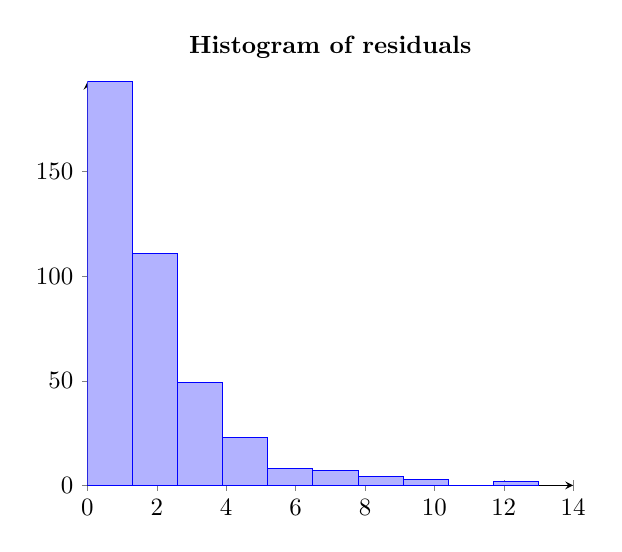
\begin{tikzpicture}[scale=0.9]
	\begin{axis}[
	ybar,
	ymin=0,
	axis y line=left,
	axis x line=bottom,
	domain=0:14,
	xmin=0,
	xmax=14,
	title=\textbf{Histogram of residuals}
	]
	\addplot +[
	hist={
		bins=10,
		data min=0,
		data max=13
	}   
	] table [y index=0] {
		dist
		3.9882
		0.8133
		0.3716
		0.7902
		3.9400
		1.9414
		0.7761
		1.3236
		0.0444
		2.6356
		0.2856
		1.9683
		3.9810
		4.9853
		0.6054
		1.9774
		1.9325
		2.3935
		2.4448
		2.6956
		1.5380
		0.0244
		1.9086
		0.1169
		3.5795
		0.1559
		0.5638
		0.3096
		1.0137
		4.4630
		1.5728
		0.8475
		5.7108
		7.7016
		2.4771
		0.1420
		1.3310
		0.2664
		1.9452
		0.2454
		1.2518
		0.2272
		4.5507
		3.1019
		0.7088
		2.0358
		13.1487
		1.9126
		2.2780
		1.8661
		3.4157
		3.1272
		1.0427
		1.0402
		3.5151
		0.1387
		5.7571
		3.2017
		1.3536
		0.5509
		3.8476
		0.1428
		1.7257
		5.7471
		0.7885
		2.5473
		0.4967
		0.0757
		0.7472
		1.3926
		4.6246
		2.4913
		1.2394
		8.9606
		2.5257
		1.0567
		3.5200
		3.5428
		0.7821
		1.1257
		1.1896
		0.0662
		0.9291
		2.2506
		1.3040
		0.2902
		0.0118
		0.3523
		2.1146
		0.5769
		0.1250
		0.8067
		1.4629
		2.5024
		1.0379
		2.1789
		0.0826
		1.6326
		0.0775
		0.7820
		0.6961
		0.0865
		0.1240
		0.3636
		3.7255
		0.3716
		1.5351
		2.4167
		1.2952
		0.3687
		1.2356
		2.6954
		2.0767
		3.3561
		2.0959
		3.3244
		0.3590
		1.9134
		9.3130
		2.3487
		0.3565
		2.5364
		0.4935
		1.2641
		3.7427
		1.2877
		2.5229
		0.6713
		0.6174
		1.5986
		3.4066
		3.9970
		2.5982
		0.9062
		0.4309
		0.8073
		2.4994
		3.8976
		2.8059
		0.7366
		5.2692
		1.3917
		0.0282
		0.1999
		1.1060
		0.5318
		0.5840
		0.7267
		0.7792
		2.5289
		1.0830
		0.9597
		0.4110
		8.2720
		3.0803
		0.0244
		0.4034
		0.9175
		0.7650
		0.4258
		2.5483
		0.8160
		7.0587
		1.2162
		1.2736
		0.2713
		3.3468
		0.1420
		0.0479
		2.2100
		0.9441
		1.2809
		1.5571
		2.0513
		2.1916
		4.9731
		1.8812
		2.8597
		1.4420
		0.7131
		3.9716
		0.3812
		0.1450
		0.3757
		1.4474
		0.8317
		1.5688
		1.7423
		6.7454
		0.1519
		6.2755
		1.4844
		1.9051
		1.2545
		0.0037
		0.2052
		8.4323
		0.4956
		1.4460
		1.8821
		0.3894
		0.2684
		0.0033
		3.2627
		0.2786
		2.3586
		1.7772
		0.4058
		1.9980
		1.7056
		4.7890
		0.8084
		0.6258
		2.4025
		2.1694
		0.6176
		0.0293
		0.7169
		4.8174
		1.5069
		0.9071
		1.2877
		3.9132
		2.5782
		0.0260
		0.4588
		0.1380
		2.1090
		3.1296
		0.7703
		2.0689
		1.6494
		0.1913
		0.3640
		1.8761
		0.6185
		2.4712
		2.4611
		2.4294
		7.3904
		0.1715
		0.7537
		2.9025
		1.3969
		0.4700
		1.9339
		3.0412
		0.6496
		0.5154
		0.7326
		0.9571
		0.5428
		1.3409
		2.2209
		13.2241
		1.0872
		3.5224
		3.2705
		3.7900
		1.3647
		8.1041
		1.5049
		6.1549
		1.6317
		3.6212
		1.1169
		0.4010
		4.9222
		2.9148
		2.8045
		2.0886
		1.7877
		4.3389
		1.7968
		0.7833
		1.2212
		2.0593
		0.8262
		0.7751
		4.0566
		1.6437
		0.1297
		1.1235
		1.0976
		0.5368
		2.7971
		0.7310
		2.4425
		1.1218
		0.9089
		1.8381
		2.7815
		0.1337
		1.6019
		1.2630
		0.9088
		0.8066
		1.6465
		3.5091
		0.7295
		0.1561
		1.9852
		0.8964
		0.2338
		1.4557
		0.9246
		1.5314
		4.4296
		4.3587
		4.4532
		1.6161
		0.1262
		0.9120
		0.1459
		5.5332
		2.3622
		0.1031
		9.1388
		3.5696
		0.5614
		0.3635
		1.0022
		1.3159
		0.1177
		0.5990
		0.7103
		0.5895
		0.2697
		0.0731
		0.0365
		0.1697
		2.5212
		5.6732
		0.3945
		3.4349
		6.7087
		0.5193
		1.2304
		2.2080
		1.0956
		0.3145
		0.8852
		1.7345
		1.2106
		3.4042
		2.8855
		3.1655
		2.6966
		0.1182
		0.8877
		0.3749
		1.8896
		3.5627
		0.6019
		0.2721
		2.0683
		3.4427
		0.0072
		0.0835
		3.7158
		0.1474
		1.7133
		3.0004
		3.9844
		2.6928
		1.2159
		4.9970
		1.0279
		7.0681
		1.5753
		2.2022
		0.1160
		2.3874
		1.6962
		0.8279
		1.9294
		3.9877
		4.6738
		2.3738
		0.3875
		0.9328
		3.1604
		0.0400
		1.6521
		0.3602
		1.2354
		7.3676
		9.9745
		0.4814
		1.6086
		2.4845
		0.2943
		0.8425
		2.5127
		0.8784
		2.6668
		3.4885
		1.9960
		1.2415
		0.1529
	};
	\end{axis}
	\end{tikzpicture}
	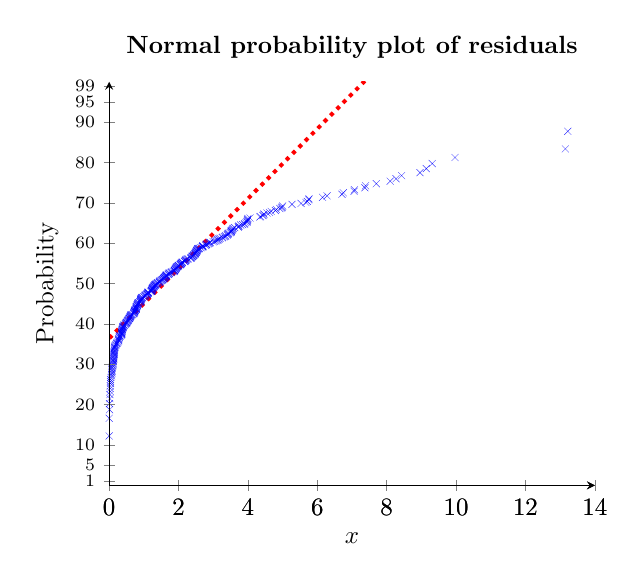
\begin{tikzpicture}[scale=0.9]
	\begin{axis}[
	xmin=0, xmax=14, xlabel=$x$,
	ymin=-4, ymax=4, ylabel=$y$,
	samples=400,
	axis x line=bottom,
	axis y line=none,
	domain=-6:-6,
	title=\textbf{Normal probability plot of residuals}
	]
	\addplot[mark=x,blue, only marks, ultra thin] coordinates {
		(0.00,-3.02)
		(0.00,-2.67)
		(0.01,-2.50)
		(0.01,-2.38)
		(0.02,-2.28)
		(0.02,-2.20)
		(0.03,-2.14)
		(0.03,-2.08)
		(0.03,-2.03)
		(0.04,-1.98)
		(0.04,-1.94)
		(0.04,-1.90)
		(0.05,-1.86)
		(0.07,-1.83)
		(0.07,-1.80)
		(0.08,-1.77)
		(0.08,-1.74)
		(0.08,-1.71)
		(0.08,-1.68)
		(0.09,-1.66)
		(0.10,-1.63)
		(0.12,-1.61)
		(0.12,-1.59)
		(0.12,-1.57)
		(0.12,-1.54)
		(0.12,-1.52)
		(0.13,-1.50)
		(0.13,-1.49)
		(0.13,-1.47)
		(0.13,-1.45)
		(0.14,-1.43)
		(0.14,-1.41)
		(0.14,-1.40)
		(0.14,-1.38)
		(0.14,-1.36)
		(0.15,-1.35)
		(0.15,-1.33)
		(0.15,-1.32)
		(0.15,-1.30)
		(0.15,-1.29)
		(0.16,-1.27)
		(0.16,-1.26)
		(0.17,-1.25)
		(0.17,-1.23)
		(0.19,-1.22)
		(0.20,-1.21)
		(0.21,-1.19)
		(0.23,-1.18)
		(0.23,-1.17)
		(0.25,-1.16)
		(0.27,-1.14)
		(0.27,-1.13)
		(0.27,-1.12)
		(0.27,-1.11)
		(0.27,-1.10)
		(0.28,-1.09)
		(0.29,-1.07)
		(0.29,-1.06)
		(0.29,-1.05)
		(0.31,-1.04)
		(0.31,-1.03)
		(0.35,-1.02)
		(0.36,-1.01)
		(0.36,-1.00)
		(0.36,-0.99)
		(0.36,-0.98)
		(0.36,-0.97)
		(0.36,-0.96)
		(0.37,-0.95)
		(0.37,-0.94)
		(0.37,-0.93)
		(0.37,-0.92)
		(0.38,-0.91)
		(0.38,-0.90)
		(0.39,-0.89)
		(0.39,-0.88)
		(0.39,-0.87)
		(0.40,-0.86)
		(0.40,-0.86)
		(0.41,-0.85)
		(0.41,-0.84)
		(0.43,-0.83)
		(0.43,-0.82)
		(0.46,-0.81)
		(0.47,-0.80)
		(0.48,-0.79)
		(0.49,-0.78)
		(0.50,-0.78)
		(0.50,-0.77)
		(0.52,-0.76)
		(0.52,-0.75)
		(0.53,-0.74)
		(0.54,-0.73)
		(0.54,-0.73)
		(0.55,-0.72)
		(0.56,-0.71)
		(0.56,-0.70)
		(0.58,-0.69)
		(0.58,-0.69)
		(0.59,-0.68)
		(0.60,-0.67)
		(0.60,-0.66)
		(0.61,-0.65)
		(0.62,-0.65)
		(0.62,-0.64)
		(0.62,-0.63)
		(0.63,-0.62)
		(0.65,-0.62)
		(0.67,-0.61)
		(0.70,-0.60)
		(0.71,-0.59)
		(0.71,-0.59)
		(0.71,-0.58)
		(0.72,-0.57)
		(0.73,-0.56)
		(0.73,-0.56)
		(0.73,-0.55)
		(0.73,-0.54)
		(0.74,-0.54)
		(0.75,-0.53)
		(0.75,-0.52)
		(0.77,-0.51)
		(0.77,-0.51)
		(0.78,-0.50)
		(0.78,-0.49)
		(0.78,-0.49)
		(0.78,-0.48)
		(0.78,-0.47)
		(0.78,-0.46)
		(0.79,-0.46)
		(0.79,-0.45)
		(0.81,-0.44)
		(0.81,-0.44)
		(0.81,-0.43)
		(0.81,-0.42)
		(0.81,-0.42)
		(0.82,-0.41)
		(0.83,-0.40)
		(0.83,-0.40)
		(0.83,-0.39)
		(0.84,-0.38)
		(0.85,-0.38)
		(0.88,-0.37)
		(0.89,-0.36)
		(0.89,-0.36)
		(0.90,-0.35)
		(0.91,-0.34)
		(0.91,-0.34)
		(0.91,-0.33)
		(0.91,-0.32)
		(0.91,-0.32)
		(0.92,-0.31)
		(0.92,-0.30)
		(0.93,-0.30)
		(0.93,-0.29)
		(0.94,-0.28)
		(0.96,-0.28)
		(0.96,-0.27)
		(1.00,-0.26)
		(1.01,-0.26)
		(1.03,-0.25)
		(1.04,-0.24)
		(1.04,-0.24)
		(1.04,-0.23)
		(1.06,-0.22)
		(1.08,-0.22)
		(1.09,-0.21)
		(1.10,-0.21)
		(1.10,-0.20)
		(1.11,-0.19)
		(1.12,-0.19)
		(1.12,-0.18)
		(1.12,-0.17)
		(1.13,-0.17)
		(1.19,-0.16)
		(1.21,-0.15)
		(1.22,-0.15)
		(1.22,-0.14)
		(1.22,-0.14)
		(1.23,-0.13)
		(1.24,-0.12)
		(1.24,-0.12)
		(1.24,-0.11)
		(1.24,-0.10)
		(1.25,-0.10)
		(1.25,-0.09)
		(1.26,-0.08)
		(1.26,-0.08)
		(1.27,-0.07)
		(1.28,-0.07)
		(1.29,-0.06)
		(1.29,-0.05)
		(1.30,-0.05)
		(1.30,-0.04)
		(1.32,-0.03)
		(1.32,-0.03)
		(1.33,-0.02)
		(1.34,-0.02)
		(1.35,-0.01)
		(1.36,-0.00)
		(1.39,0.00)
		(1.39,0.01)
		(1.40,0.02)
		(1.44,0.02)
		(1.45,0.03)
		(1.45,0.03)
		(1.46,0.04)
		(1.46,0.05)
		(1.48,0.05)
		(1.50,0.06)
		(1.51,0.07)
		(1.53,0.07)
		(1.54,0.08)
		(1.54,0.08)
		(1.56,0.09)
		(1.57,0.10)
		(1.57,0.10)
		(1.58,0.11)
		(1.60,0.12)
		(1.60,0.12)
		(1.61,0.13)
		(1.62,0.14)
		(1.63,0.14)
		(1.63,0.15)
		(1.64,0.15)
		(1.65,0.16)
		(1.65,0.17)
		(1.65,0.17)
		(1.70,0.18)
		(1.71,0.19)
		(1.71,0.19)
		(1.73,0.20)
		(1.73,0.21)
		(1.74,0.21)
		(1.78,0.22)
		(1.79,0.22)
		(1.80,0.23)
		(1.84,0.24)
		(1.87,0.24)
		(1.88,0.25)
		(1.88,0.26)
		(1.88,0.26)
		(1.89,0.27)
		(1.91,0.28)
		(1.91,0.28)
		(1.91,0.29)
		(1.91,0.30)
		(1.93,0.30)
		(1.93,0.31)
		(1.93,0.32)
		(1.94,0.32)
		(1.95,0.33)
		(1.97,0.34)
		(1.98,0.34)
		(1.99,0.35)
		(2.00,0.36)
		(2.00,0.36)
		(2.04,0.37)
		(2.05,0.38)
		(2.06,0.38)
		(2.07,0.39)
		(2.07,0.40)
		(2.08,0.40)
		(2.09,0.41)
		(2.10,0.42)
		(2.11,0.42)
		(2.11,0.43)
		(2.17,0.44)
		(2.18,0.44)
		(2.19,0.45)
		(2.20,0.46)
		(2.21,0.46)
		(2.21,0.47)
		(2.22,0.48)
		(2.25,0.49)
		(2.28,0.49)
		(2.35,0.50)
		(2.36,0.51)
		(2.36,0.51)
		(2.37,0.52)
		(2.39,0.53)
		(2.39,0.54)
		(2.40,0.54)
		(2.42,0.55)
		(2.43,0.56)
		(2.44,0.56)
		(2.44,0.57)
		(2.46,0.58)
		(2.47,0.59)
		(2.48,0.59)
		(2.48,0.60)
		(2.49,0.61)
		(2.50,0.62)
		(2.50,0.62)
		(2.51,0.63)
		(2.52,0.64)
		(2.52,0.65)
		(2.53,0.65)
		(2.53,0.66)
		(2.54,0.67)
		(2.55,0.68)
		(2.55,0.69)
		(2.58,0.69)
		(2.60,0.70)
		(2.64,0.71)
		(2.67,0.72)
		(2.69,0.73)
		(2.70,0.73)
		(2.70,0.74)
		(2.70,0.75)
		(2.78,0.76)
		(2.80,0.77)
		(2.80,0.78)
		(2.81,0.78)
		(2.86,0.79)
		(2.89,0.80)
		(2.90,0.81)
		(2.91,0.82)
		(3.00,0.83)
		(3.04,0.84)
		(3.08,0.85)
		(3.10,0.86)
		(3.13,0.86)
		(3.13,0.87)
		(3.16,0.88)
		(3.17,0.89)
		(3.20,0.90)
		(3.26,0.91)
		(3.27,0.92)
		(3.32,0.93)
		(3.35,0.94)
		(3.36,0.95)
		(3.40,0.96)
		(3.41,0.97)
		(3.42,0.98)
		(3.43,0.99)
		(3.44,1.00)
		(3.49,1.01)
		(3.51,1.02)
		(3.52,1.03)
		(3.52,1.04)
		(3.52,1.05)
		(3.54,1.06)
		(3.56,1.07)
		(3.57,1.09)
		(3.58,1.10)
		(3.62,1.11)
		(3.72,1.12)
		(3.73,1.13)
		(3.74,1.14)
		(3.79,1.16)
		(3.85,1.17)
		(3.90,1.18)
		(3.91,1.19)
		(3.94,1.21)
		(3.97,1.22)
		(3.98,1.23)
		(3.98,1.25)
		(3.99,1.26)
		(3.99,1.27)
		(4.00,1.29)
		(4.06,1.30)
		(4.34,1.32)
		(4.36,1.33)
		(4.43,1.35)
		(4.45,1.36)
		(4.46,1.38)
		(4.55,1.40)
		(4.62,1.41)
		(4.67,1.43)
		(4.79,1.45)
		(4.82,1.47)
		(4.92,1.49)
		(4.97,1.50)
		(4.99,1.52)
		(5.00,1.54)
		(5.27,1.57)
		(5.53,1.59)
		(5.67,1.61)
		(5.71,1.63)
		(5.75,1.66)
		(5.76,1.68)
		(6.15,1.71)
		(6.28,1.74)
		(6.71,1.77)
		(6.75,1.80)
		(7.06,1.83)
		(7.07,1.86)
		(7.37,1.90)
		(7.39,1.94)
		(7.70,1.98)
		(8.10,2.03)
		(8.27,2.08)
		(8.43,2.14)
		(8.96,2.20)
		(9.14,2.28)
		(9.31,2.38)
		(9.97,2.50)
		(13.15,2.67)
		(13.22,3.02)
	};
	\addplot[dotted,red,ultra thick] coordinates {
		(0.0033,-1.0838)
		(13.2241,8.0734)
	};
	\end{axis}
	\begin{axis}[
	xmin=0,
	xmax=14,
	ymin=0,
	ymax=100,
	ylabel=Probability,
	axis y line=left,
	axis x line=bottom,
	yticklabel style={font=\scriptsize},
	ytick={1,5,10,20,30,40,50,60,70,80,90,95,99},
	]
	\end{axis}
	\end{tikzpicture}
\end{center}
\begin{center}
	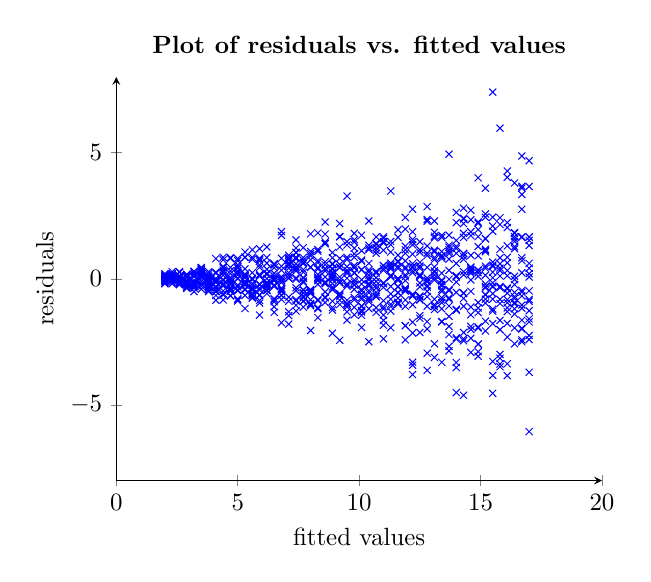
\begin{tikzpicture}[scale=0.9]
	\begin{axis}[
		xmin=0, xmax=20, xlabel=fitted values,
		ymin=-8, ymax=8, ylabel=residuals,
		samples=400,
		axis x line=bottom,
		axis y line=left,
		domain=0:20,
		title=\textbf{Plot of residuals vs. fitted values}
	]
		\addplot[mark=x,blue, only marks] coordinates {
			(2.00,0.06)
			(2.00,-0.09)
			(2.00,-0.17)
			(2.00,-0.08)
			(2.00,0.15)
			(2.00,0.05)
			(2.00,-0.11)
			(2.00,0.13)
			(2.00,-0.08)
			(2.00,-0.00)
			(2.00,-0.07)
			(2.00,-0.00)
			(2.00,-0.07)
			(2.00,-0.07)
			(2.00,-0.07)
			(2.00,0.20)
			(2.00,-0.20)
			(2.00,0.10)
			(2.00,-0.05)
			(2.00,0.06)
			(2.30,0.14)
			(2.30,-0.20)
			(2.30,0.10)
			(2.30,-0.04)
			(2.30,-0.14)
			(2.30,-0.00)
			(2.30,-0.01)
			(2.30,0.04)
			(2.30,0.06)
			(2.30,-0.04)
			(2.30,0.10)
			(2.30,0.04)
			(2.30,0.18)
			(2.30,0.20)
			(2.30,-0.07)
			(2.30,-0.04)
			(2.30,0.15)
			(2.30,0.28)
			(2.30,0.18)
			(2.30,-0.00)
			(2.60,0.04)
			(2.60,0.28)
			(2.60,-0.20)
			(2.60,-0.04)
			(2.60,-0.14)
			(2.60,0.25)
			(2.60,-0.22)
			(2.60,-0.09)
			(2.60,0.01)
			(2.60,0.06)
			(2.60,-0.07)
			(2.60,-0.18)
			(2.60,-0.06)
			(2.60,-0.06)
			(2.60,-0.21)
			(2.60,-0.24)
			(2.60,0.04)
			(2.60,0.12)
			(2.60,0.09)
			(2.60,-0.00)
			(2.90,-0.13)
			(2.90,-0.35)
			(2.90,-0.22)
			(2.90,-0.13)
			(2.90,-0.06)
			(2.90,0.05)
			(2.90,0.05)
			(2.90,0.18)
			(2.90,0.07)
			(2.90,-0.30)
			(2.90,0.17)
			(2.90,-0.23)
			(2.90,-0.10)
			(2.90,-0.16)
			(2.90,0.13)
			(2.90,-0.38)
			(2.90,0.12)
			(2.90,-0.16)
			(2.90,-0.19)
			(2.90,-0.29)
			(3.20,-0.22)
			(3.20,-0.32)
			(3.20,-0.24)
			(3.20,0.29)
			(3.20,-0.06)
			(3.20,-0.28)
			(3.20,0.29)
			(3.20,0.14)
			(3.20,0.08)
			(3.20,-0.15)
			(3.20,0.16)
			(3.20,-0.17)
			(3.20,-0.21)
			(3.20,-0.16)
			(3.20,-0.13)
			(3.20,0.12)
			(3.20,0.22)
			(3.20,-0.51)
			(3.20,-0.13)
			(3.20,-0.37)
			(3.50,0.34)
			(3.50,0.45)
			(3.50,-0.20)
			(3.50,0.24)
			(3.50,0.15)
			(3.50,0.10)
			(3.50,0.26)
			(3.50,0.21)
			(3.50,0.06)
			(3.50,-0.22)
			(3.50,0.43)
			(3.50,-0.30)
			(3.50,-0.03)
			(3.50,-0.11)
			(3.50,0.29)
			(3.50,0.34)
			(3.50,0.37)
			(3.50,0.41)
			(3.50,-0.41)
			(3.50,0.10)
			(3.80,0.00)
			(3.80,-0.21)
			(3.80,0.06)
			(3.80,-0.10)
			(3.80,-0.41)
			(3.80,-0.26)
			(3.80,-0.32)
			(3.80,-0.30)
			(3.80,-0.04)
			(3.80,0.06)
			(3.80,-0.32)
			(3.80,-0.51)
			(3.80,-0.35)
			(3.80,0.20)
			(3.80,0.28)
			(3.80,-0.47)
			(3.80,0.11)
			(3.80,-0.15)
			(3.80,-0.31)
			(3.80,0.09)
			(4.10,-0.51)
			(4.10,-0.51)
			(4.10,-0.14)
			(4.10,-0.85)
			(4.10,-0.30)
			(4.10,-0.49)
			(4.10,-0.66)
			(4.10,-0.33)
			(4.10,0.01)
			(4.10,-0.12)
			(4.10,0.80)
			(4.10,-0.07)
			(4.10,-0.33)
			(4.10,0.26)
			(4.10,0.22)
			(4.10,-0.35)
			(4.10,-0.05)
			(4.10,-0.43)
			(4.10,-0.14)
			(4.10,-0.12)
			(4.40,0.85)
			(4.40,0.27)
			(4.40,-0.48)
			(4.40,-0.59)
			(4.40,-0.29)
			(4.40,0.14)
			(4.40,0.75)
			(4.40,-0.25)
			(4.40,-0.07)
			(4.40,-0.64)
			(4.40,0.49)
			(4.40,0.24)
			(4.40,0.35)
			(4.40,0.29)
			(4.40,-0.84)
			(4.40,0.45)
			(4.40,-0.03)
			(4.40,-0.25)
			(4.40,-0.19)
			(4.40,0.44)
			(4.70,0.84)
			(4.70,0.45)
			(4.70,0.80)
			(4.70,-0.24)
			(4.70,-0.68)
			(4.70,-0.17)
			(4.70,-0.48)
			(4.70,-0.49)
			(4.70,-0.17)
			(4.70,-0.66)
			(4.70,-0.40)
			(4.70,-0.05)
			(4.70,0.05)
			(4.70,-0.35)
			(4.70,-0.12)
			(4.70,-0.01)
			(4.70,-0.16)
			(4.70,0.31)
			(4.70,-0.40)
			(4.70,0.20)
			(5.00,0.72)
			(5.00,0.80)
			(5.00,-0.25)
			(5.00,0.24)
			(5.00,-0.47)
			(5.00,0.22)
			(5.00,-0.80)
			(5.00,-0.83)
			(5.00,-0.44)
			(5.00,-0.88)
			(5.00,0.24)
			(5.00,0.03)
			(5.00,0.47)
			(5.00,0.15)
			(5.00,0.31)
			(5.00,-0.47)
			(5.00,0.42)
			(5.00,-0.01)
			(5.00,-0.32)
			(5.00,0.55)
			(5.30,0.39)
			(5.30,-0.10)
			(5.30,0.14)
			(5.30,-0.19)
			(5.30,-0.44)
			(5.30,0.11)
			(5.30,-0.14)
			(5.30,-0.20)
			(5.30,0.19)
			(5.30,-0.25)
			(5.30,-0.17)
			(5.30,0.86)
			(5.30,-1.18)
			(5.30,-0.40)
			(5.30,-0.66)
			(5.30,1.06)
			(5.30,-0.13)
			(5.30,0.85)
			(5.30,0.09)
			(5.30,0.03)
			(5.60,-0.65)
			(5.60,-0.60)
			(5.60,-0.04)
			(5.60,-0.35)
			(5.60,1.15)
			(5.60,-0.64)
			(5.60,0.77)
			(5.60,0.24)
			(5.60,-0.19)
			(5.60,-0.58)
			(5.60,-0.42)
			(5.60,-0.38)
			(5.60,-0.75)
			(5.60,0.85)
			(5.60,-0.45)
			(5.60,-0.68)
			(5.60,0.01)
			(5.60,0.01)
			(5.60,-0.77)
			(5.60,-0.26)
			(5.90,0.14)
			(5.90,0.76)
			(5.90,-0.21)
			(5.90,0.55)
			(5.90,-0.96)
			(5.90,-0.24)
			(5.90,0.10)
			(5.90,-1.44)
			(5.90,0.13)
			(5.90,-0.37)
			(5.90,-0.66)
			(5.90,0.70)
			(5.90,0.17)
			(5.90,-0.45)
			(5.90,-0.22)
			(5.90,-0.86)
			(5.90,-0.63)
			(5.90,0.81)
			(5.90,1.19)
			(5.90,0.45)
			(6.20,-0.47)
			(6.20,0.22)
			(6.20,-0.34)
			(6.20,-0.45)
			(6.20,0.62)
			(6.20,1.26)
			(6.20,0.17)
			(6.20,0.62)
			(6.20,-0.44)
			(6.20,-0.17)
			(6.20,-0.21)
			(6.20,0.84)
			(6.20,-0.28)
			(6.20,0.01)
			(6.20,0.38)
			(6.20,-0.27)
			(6.20,-0.59)
			(6.20,-0.14)
			(6.20,-0.45)
			(6.20,-0.34)
			(6.50,0.59)
			(6.50,-0.07)
			(6.50,0.55)
			(6.50,-0.91)
			(6.50,-0.07)
			(6.50,-0.83)
			(6.50,-0.01)
			(6.50,-0.79)
			(6.50,0.22)
			(6.50,0.56)
			(6.50,-0.29)
			(6.50,0.11)
			(6.50,0.57)
			(6.50,0.44)
			(6.50,0.03)
			(6.50,-1.11)
			(6.50,-0.30)
			(6.50,-1.33)
			(6.50,-0.25)
			(6.50,0.59)
			(6.80,0.34)
			(6.80,1.72)
			(6.80,-0.14)
			(6.80,0.50)
			(6.80,0.08)
			(6.80,-0.66)
			(6.80,0.02)
			(6.80,-0.40)
			(6.80,-0.65)
			(6.80,-0.43)
			(6.80,-0.14)
			(6.80,1.87)
			(6.80,-0.37)
			(6.80,-0.49)
			(6.80,-0.51)
			(6.80,-0.00)
			(6.80,0.81)
			(6.80,-0.82)
			(6.80,-1.74)
			(6.80,-0.06)
			(7.10,0.74)
			(7.10,-1.80)
			(7.10,0.57)
			(7.10,0.93)
			(7.10,0.13)
			(7.10,-1.46)
			(7.10,0.01)
			(7.10,0.42)
			(7.10,0.62)
			(7.10,0.53)
			(7.10,0.55)
			(7.10,0.84)
			(7.10,-0.89)
			(7.10,0.77)
			(7.10,-1.31)
			(7.10,0.04)
			(7.10,0.24)
			(7.10,0.82)
			(7.10,-0.73)
			(7.10,0.14)
			(7.40,1.05)
			(7.40,0.31)
			(7.40,0.59)
			(7.40,-0.02)
			(7.40,-0.47)
			(7.40,0.79)
			(7.40,0.47)
			(7.40,0.85)
			(7.40,-0.36)
			(7.40,0.04)
			(7.40,0.82)
			(7.40,-0.83)
			(7.40,0.44)
			(7.40,0.37)
			(7.40,1.22)
			(7.40,1.54)
			(7.40,1.03)
			(7.40,-0.88)
			(7.40,-1.28)
			(7.40,-1.05)
			(7.70,0.60)
			(7.70,-0.44)
			(7.70,-0.88)
			(7.70,-0.15)
			(7.70,-0.09)
			(7.70,-1.12)
			(7.70,0.02)
			(7.70,-0.90)
			(7.70,-0.69)
			(7.70,0.74)
			(7.70,-0.44)
			(7.70,-0.57)
			(7.70,1.23)
			(7.70,0.84)
			(7.70,0.36)
			(7.70,0.26)
			(7.70,-0.75)
			(7.70,-0.56)
			(7.70,0.65)
			(7.70,0.05)
			(8.00,-0.47)
			(8.00,1.78)
			(8.00,-0.51)
			(8.00,-0.57)
			(8.00,-0.43)
			(8.00,-2.05)
			(8.00,0.45)
			(8.00,0.91)
			(8.00,0.46)
			(8.00,-1.03)
			(8.00,-1.07)
			(8.00,0.75)
			(8.00,-0.55)
			(8.00,0.99)
			(8.00,-0.98)
			(8.00,0.46)
			(8.00,-0.83)
			(8.00,-0.46)
			(8.00,-0.58)
			(8.00,1.08)
			(8.30,0.72)
			(8.30,0.17)
			(8.30,1.16)
			(8.30,-0.86)
			(8.30,-1.54)
			(8.30,0.39)
			(8.30,0.05)
			(8.30,0.06)
			(8.30,-0.83)
			(8.30,0.64)
			(8.30,0.45)
			(8.30,-1.19)
			(8.30,-0.04)
			(8.30,1.09)
			(8.30,-0.08)
			(8.30,1.82)
			(8.30,0.06)
			(8.30,-0.22)
			(8.30,-1.15)
			(8.30,0.02)
			(8.60,0.56)
			(8.60,1.77)
			(8.60,-0.76)
			(8.60,-0.20)
			(8.60,0.07)
			(8.60,0.31)
			(8.60,0.40)
			(8.60,1.39)
			(8.60,0.67)
			(8.60,-0.52)
			(8.60,2.25)
			(8.60,-0.52)
			(8.60,0.40)
			(8.60,1.40)
			(8.60,1.46)
			(8.60,-0.94)
			(8.60,-0.16)
			(8.60,-0.72)
			(8.60,-0.13)
			(8.60,-0.15)
			(8.90,-1.24)
			(8.90,0.37)
			(8.90,0.41)
			(8.90,-0.19)
			(8.90,-0.43)
			(8.90,-0.33)
			(8.90,-2.16)
			(8.90,-1.14)
			(8.90,-0.89)
			(8.90,0.15)
			(8.90,0.22)
			(8.90,-0.41)
			(8.90,0.57)
			(8.90,0.25)
			(8.90,0.83)
			(8.90,-0.04)
			(8.90,0.09)
			(8.90,0.60)
			(8.90,0.03)
			(8.90,1.04)
			(9.20,-0.63)
			(9.20,0.46)
			(9.20,-0.15)
			(9.20,0.44)
			(9.20,-0.85)
			(9.20,0.81)
			(9.20,-2.44)
			(9.20,-0.70)
			(9.20,2.19)
			(9.20,1.68)
			(9.20,0.07)
			(9.20,-1.02)
			(9.20,-0.59)
			(9.20,-0.69)
			(9.20,0.57)
			(9.20,1.66)
			(9.20,-0.14)
			(9.20,-0.05)
			(9.20,-0.16)
			(9.20,1.26)
			(9.50,-0.29)
			(9.50,0.33)
			(9.50,-1.05)
			(9.50,0.77)
			(9.50,-1.31)
			(9.50,0.48)
			(9.50,-0.98)
			(9.50,3.28)
			(9.50,0.26)
			(9.50,-0.85)
			(9.50,-0.21)
			(9.50,1.34)
			(9.50,0.02)
			(9.50,-1.64)
			(9.50,0.85)
			(9.50,-0.21)
			(9.50,-0.99)
			(9.50,1.47)
			(9.50,0.21)
			(9.50,-1.12)
			(9.80,1.80)
			(9.80,1.21)
			(9.80,-1.43)
			(9.80,0.25)
			(9.80,0.85)
			(9.80,-0.83)
			(9.80,0.44)
			(9.80,-0.13)
			(9.80,-0.23)
			(9.80,-1.13)
			(9.80,1.46)
			(9.80,0.52)
			(9.80,-0.04)
			(9.80,0.22)
			(9.80,1.55)
			(9.80,-0.25)
			(9.80,-0.75)
			(9.80,0.44)
			(9.80,0.99)
			(9.80,-0.42)
			(10.10,-1.45)
			(10.10,-1.93)
			(10.10,-1.27)
			(10.10,1.73)
			(10.10,1.11)
			(10.10,-1.32)
			(10.10,-0.21)
			(10.10,0.35)
			(10.10,-0.74)
			(10.10,0.37)
			(10.10,-0.81)
			(10.10,-1.25)
			(10.10,-1.08)
			(10.10,0.69)
			(10.10,-0.49)
			(10.10,-0.43)
			(10.10,-0.04)
			(10.10,-1.10)
			(10.10,-0.61)
			(10.10,0.74)
			(10.40,1.16)
			(10.40,-0.04)
			(10.40,0.27)
			(10.40,-0.90)
			(10.40,-0.56)
			(10.40,-0.47)
			(10.40,0.61)
			(10.40,-0.29)
			(10.40,1.33)
			(10.40,-1.19)
			(10.40,0.35)
			(10.40,-0.75)
			(10.40,0.03)
			(10.40,0.14)
			(10.40,-2.50)
			(10.40,-0.24)
			(10.40,-0.81)
			(10.40,2.29)
			(10.40,1.22)
			(10.40,-0.19)
			(10.70,-0.70)
			(10.70,-0.26)
			(10.70,0.29)
			(10.70,1.23)
			(10.70,-0.11)
			(10.70,1.01)
			(10.70,-0.36)
			(10.70,1.39)
			(10.70,-0.54)
			(10.70,-1.33)
			(10.70,1.37)
			(10.70,1.12)
			(10.70,-0.63)
			(10.70,-0.71)
			(10.70,1.66)
			(10.70,-0.37)
			(10.70,0.23)
			(10.70,1.39)
			(10.70,0.04)
			(10.70,-1.15)
			(11.00,-0.34)
			(11.00,1.44)
			(11.00,-0.87)
			(11.00,1.42)
			(11.00,-0.20)
			(11.00,-1.20)
			(11.00,-1.11)
			(11.00,1.13)
			(11.00,0.41)
			(11.00,0.34)
			(11.00,-1.84)
			(11.00,1.48)
			(11.00,-0.16)
			(11.00,0.52)
			(11.00,1.66)
			(11.00,-1.44)
			(11.00,0.53)
			(11.00,-1.65)
			(11.00,-2.38)
			(11.00,1.60)
			(11.30,0.10)
			(11.30,0.55)
			(11.30,-1.28)
			(11.30,0.45)
			(11.30,-1.01)
			(11.30,0.62)
			(11.30,-1.10)
			(11.30,0.48)
			(11.30,3.48)
			(11.30,1.06)
			(11.30,-0.60)
			(11.30,-0.30)
			(11.30,-1.94)
			(11.30,0.14)
			(11.30,1.35)
			(11.30,1.48)
			(11.30,-0.81)
			(11.30,0.47)
			(11.30,0.39)
			(11.30,0.07)
			(11.60,-0.93)
			(11.60,-0.95)
			(11.60,0.01)
			(11.60,-0.55)
			(11.60,-0.56)
			(11.60,0.70)
			(11.60,0.94)
			(11.60,-0.07)
			(11.60,0.41)
			(11.60,1.64)
			(11.60,-0.77)
			(11.60,0.49)
			(11.60,0.66)
			(11.60,-0.32)
			(11.60,-0.31)
			(11.60,-0.03)
			(11.60,-0.99)
			(11.60,1.94)
			(11.60,0.01)
			(11.60,-1.01)
			(11.90,-0.44)
			(11.90,1.97)
			(11.90,-2.42)
			(11.90,0.71)
			(11.90,1.15)
			(11.90,1.01)
			(11.90,-1.86)
			(11.90,2.43)
			(11.90,-0.41)
			(11.90,0.39)
			(11.90,-0.84)
			(11.90,-0.07)
			(11.90,-1.86)
			(11.90,-0.49)
			(11.90,-1.09)
			(11.90,-0.37)
			(11.90,0.46)
			(11.90,0.08)
			(11.90,1.29)
			(11.90,0.15)
			(12.20,-3.80)
			(12.20,-0.69)
			(12.20,1.56)
			(12.20,1.46)
			(12.20,2.76)
			(12.20,-1.03)
			(12.20,1.86)
			(12.20,0.24)
			(12.20,0.98)
			(12.20,0.44)
			(12.20,0.60)
			(12.20,0.32)
			(12.20,-0.61)
			(12.20,-3.31)
			(12.20,-1.72)
			(12.20,-2.15)
			(12.20,-0.67)
			(12.20,-3.43)
			(12.20,0.49)
			(12.20,1.35)
			(12.50,-2.13)
			(12.50,-0.17)
			(12.50,-0.73)
			(12.50,-0.68)
			(12.50,1.15)
			(12.50,-0.32)
			(12.50,-0.82)
			(12.50,-1.57)
			(12.50,0.15)
			(12.50,0.42)
			(12.50,0.15)
			(12.50,0.51)
			(12.50,1.05)
			(12.50,1.47)
			(12.50,-0.84)
			(12.50,0.13)
			(12.50,0.65)
			(12.50,0.08)
			(12.50,0.49)
			(12.50,-1.46)
			(12.80,0.92)
			(12.80,-0.71)
			(12.80,-0.26)
			(12.80,2.86)
			(12.80,-0.12)
			(12.80,0.45)
			(12.80,-3.63)
			(12.80,1.30)
			(12.80,2.35)
			(12.80,-1.70)
			(12.80,-0.33)
			(12.80,-1.09)
			(12.80,-2.95)
			(12.80,-1.99)
			(12.80,-0.06)
			(12.80,0.03)
			(12.80,1.01)
			(12.80,-0.50)
			(12.80,-0.49)
			(12.80,2.28)
			(13.10,-1.10)
			(13.10,-1.22)
			(13.10,0.76)
			(13.10,0.84)
			(13.10,-0.05)
			(13.10,0.03)
			(13.10,-1.03)
			(13.10,1.84)
			(13.10,0.31)
			(13.10,1.13)
			(13.10,1.69)
			(13.10,1.07)
			(13.10,-3.12)
			(13.10,1.62)
			(13.10,-0.81)
			(13.10,0.15)
			(13.10,0.26)
			(13.10,-2.58)
			(13.10,2.29)
			(13.10,0.47)
			(13.40,1.08)
			(13.40,-0.22)
			(13.40,0.81)
			(13.40,-0.05)
			(13.40,-0.42)
			(13.40,1.64)
			(13.40,-0.10)
			(13.40,-1.69)
			(13.40,0.88)
			(13.40,-1.19)
			(13.40,-0.95)
			(13.40,-0.85)
			(13.40,1.72)
			(13.40,0.22)
			(13.40,-1.71)
			(13.40,-0.50)
			(13.40,0.92)
			(13.40,-0.28)
			(13.40,-0.75)
			(13.40,-3.31)
			(13.70,-1.89)
			(13.70,-0.02)
			(13.70,-2.86)
			(13.70,-0.76)
			(13.70,-0.81)
			(13.70,-1.08)
			(13.70,-1.49)
			(13.70,1.33)
			(13.70,-2.68)
			(13.70,1.15)
			(13.70,-0.47)
			(13.70,-0.43)
			(13.70,1.00)
			(13.70,0.78)
			(13.70,4.94)
			(13.70,-2.21)
			(13.70,1.25)
			(13.70,1.73)
			(13.70,1.08)
			(13.70,0.33)
			(14.00,1.01)
			(14.00,-4.51)
			(14.00,1.28)
			(14.00,0.61)
			(14.00,1.52)
			(14.00,-0.54)
			(14.00,0.10)
			(14.00,-0.13)
			(14.00,-2.39)
			(14.00,2.63)
			(14.00,-3.32)
			(14.00,0.07)
			(14.00,-1.21)
			(14.00,1.20)
			(14.00,0.12)
			(14.00,-3.52)
			(14.00,2.23)
			(14.00,-1.22)
			(14.00,-2.34)
			(14.00,-1.25)
			(14.30,1.00)
			(14.30,-0.58)
			(14.30,-4.62)
			(14.30,2.40)
			(14.30,-0.56)
			(14.30,1.64)
			(14.30,1.80)
			(14.30,0.77)
			(14.30,0.16)
			(14.30,2.37)
			(14.30,-2.38)
			(14.30,-1.09)
			(14.30,-2.13)
			(14.30,-0.78)
			(14.30,-2.46)
			(14.30,2.19)
			(14.30,0.28)
			(14.30,0.89)
			(14.30,1.00)
			(14.30,2.80)
			(14.60,-1.12)
			(14.60,-2.36)
			(14.60,-1.89)
			(14.60,0.93)
			(14.60,0.29)
			(14.60,0.47)
			(14.60,0.38)
			(14.60,-0.50)
			(14.60,-2.92)
			(14.60,0.34)
			(14.60,2.72)
			(14.60,-2.01)
			(14.60,1.71)
			(14.60,2.34)
			(14.60,-1.43)
			(14.60,-0.05)
			(14.60,0.44)
			(14.60,1.86)
			(14.60,1.86)
			(14.60,0.22)
			(14.90,0.24)
			(14.90,-0.94)
			(14.90,0.33)
			(14.90,-3.07)
			(14.90,0.91)
			(14.90,4.00)
			(14.90,1.95)
			(14.90,-2.59)
			(14.90,2.25)
			(14.90,-2.89)
			(14.90,2.20)
			(14.90,0.10)
			(14.90,-2.59)
			(14.90,-1.91)
			(14.90,0.35)
			(14.90,1.67)
			(14.90,-1.34)
			(14.90,-1.95)
			(14.90,-1.16)
			(14.90,1.28)
			(15.20,1.58)
			(15.20,0.14)
			(15.20,2.57)
			(15.20,-0.21)
			(15.20,1.11)
			(15.20,-1.68)
			(15.20,0.50)
			(15.20,0.42)
			(15.20,-0.81)
			(15.20,-0.64)
			(15.20,1.17)
			(15.20,1.60)
			(15.20,-2.07)
			(15.20,-0.96)
			(15.20,2.44)
			(15.20,1.07)
			(15.20,3.59)
			(15.20,-0.62)
			(15.20,-0.31)
			(15.20,-0.36)
			(15.50,-0.29)
			(15.50,2.09)
			(15.50,1.88)
			(15.50,7.40)
			(15.50,2.44)
			(15.50,-3.83)
			(15.50,-1.20)
			(15.50,0.49)
			(15.50,-1.28)
			(15.50,-0.59)
			(15.50,-0.16)
			(15.50,-0.81)
			(15.50,-3.28)
			(15.50,0.04)
			(15.50,-1.78)
			(15.50,0.54)
			(15.50,-4.54)
			(15.50,0.26)
			(15.50,-0.32)
			(15.50,0.66)
			(15.80,-0.98)
			(15.80,-2.02)
			(15.80,-0.30)
			(15.80,0.42)
			(15.80,-1.65)
			(15.80,-2.02)
			(15.80,-0.82)
			(15.80,-3.15)
			(15.80,-3.38)
			(15.80,-3.49)
			(15.80,0.59)
			(15.80,0.32)
			(15.80,0.11)
			(15.80,5.97)
			(15.80,0.83)
			(15.80,1.17)
			(15.80,-0.35)
			(15.80,-3.00)
			(15.80,2.42)
			(15.80,2.15)
			(16.10,0.85)
			(16.10,-3.84)
			(16.10,1.30)
			(16.10,0.63)
			(16.10,4.02)
			(16.10,0.12)
			(16.10,-1.30)
			(16.10,-1.77)
			(16.10,-0.57)
			(16.10,-0.83)
			(16.10,2.03)
			(16.10,4.27)
			(16.10,-2.31)
			(16.10,-0.36)
			(16.10,-0.40)
			(16.10,-3.37)
			(16.10,0.33)
			(16.10,-0.95)
			(16.10,-1.15)
			(16.10,2.23)
			(16.40,1.27)
			(16.40,-1.40)
			(16.40,1.67)
			(16.40,-0.71)
			(16.40,-1.19)
			(16.40,-0.03)
			(16.40,-1.95)
			(16.40,-0.78)
			(16.40,-0.99)
			(16.40,-0.54)
			(16.40,-0.23)
			(16.40,3.80)
			(16.40,1.48)
			(16.40,-0.94)
			(16.40,1.81)
			(16.40,1.58)
			(16.40,1.83)
			(16.40,0.10)
			(16.40,-2.58)
			(16.40,1.19)
			(16.70,0.72)
			(16.70,-1.96)
			(16.70,3.67)
			(16.70,-0.68)
			(16.70,1.64)
			(16.70,-1.99)
			(16.70,2.76)
			(16.70,-0.53)
			(16.70,-1.04)
			(16.70,1.67)
			(16.70,-0.46)
			(16.70,3.34)
			(16.70,3.60)
			(16.70,0.24)
			(16.70,4.87)
			(16.70,-1.17)
			(16.70,-1.64)
			(16.70,-2.50)
			(16.70,-2.43)
			(16.70,0.83)
			(17.00,-0.82)
			(17.00,1.52)
			(17.00,0.61)
			(17.00,-1.27)
			(17.00,-0.89)
			(17.00,-1.71)
			(17.00,0.42)
			(17.00,-0.48)
			(17.00,1.65)
			(17.00,-6.06)
			(17.00,3.66)
			(17.00,-2.25)
			(17.00,1.66)
			(17.00,-3.71)
			(17.00,1.32)
			(17.00,-2.41)
			(17.00,4.68)
			(17.00,0.07)
			(17.00,0.20)
			(17.00,-1.59)
		};
	\end{axis}
	\end{tikzpicture}
	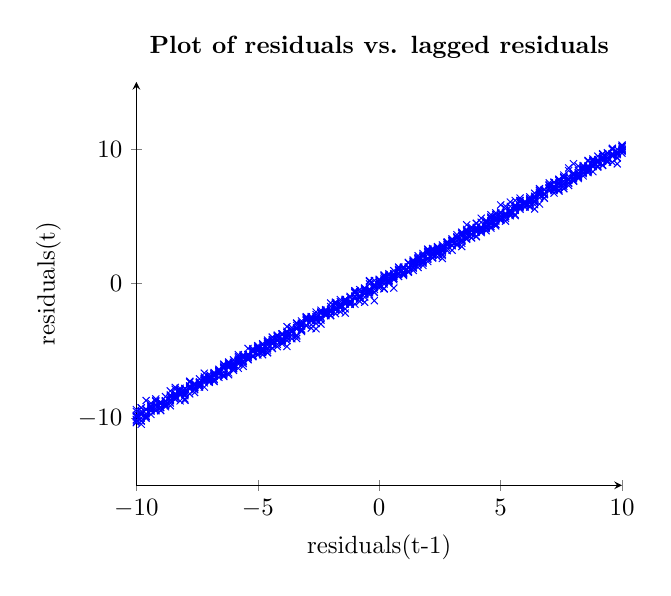
\begin{tikzpicture}[scale=0.9]
	\begin{axis}[
	xmin=-10, xmax=10, xlabel=residuals(t-1),
	ymin=-15, ymax=15, ylabel=residuals(t),
	samples=400,
	axis x line=bottom,
	axis y line=left,
	domain=-10:10,
	title=\textbf{Plot of residuals vs. lagged residuals}
	]
	\addplot[mark=x,blue, only marks] coordinates {
		(-10.00,-10.34)
		(-10.00,-10.28)
		(-10.00,-9.79)
		(-10.00,-10.14)
		(-10.00,-9.52)
		(-10.00,-9.84)
		(-10.00,-9.90)
		(-10.00,-9.37)
		(-10.00,-10.12)
		(-10.00,-9.89)
		(-9.80,-9.62)
		(-9.80,-9.99)
		(-9.80,-9.74)
		(-9.80,-10.23)
		(-9.80,-9.49)
		(-9.80,-9.23)
		(-9.80,-9.71)
		(-9.80,-10.46)
		(-9.80,-9.24)
		(-9.80,-10.18)
		(-9.60,-9.98)
		(-9.60,-9.86)
		(-9.60,-9.68)
		(-9.60,-10.02)
		(-9.60,-8.69)
		(-9.60,-9.88)
		(-9.60,-9.33)
		(-9.60,-9.39)
		(-9.60,-9.85)
		(-9.60,-9.88)
		(-9.40,-8.90)
		(-9.40,-9.18)
		(-9.40,-9.73)
		(-9.40,-9.48)
		(-9.40,-9.43)
		(-9.40,-9.21)
		(-9.40,-9.11)
		(-9.40,-9.10)
		(-9.40,-9.11)
		(-9.40,-9.31)
		(-9.20,-8.70)
		(-9.20,-9.45)
		(-9.20,-8.58)
		(-9.20,-9.00)
		(-9.20,-8.76)
		(-9.20,-9.27)
		(-9.20,-9.43)
		(-9.20,-9.04)
		(-9.20,-9.06)
		(-9.20,-9.05)
		(-9.00,-8.94)
		(-9.00,-8.80)
		(-9.00,-8.85)
		(-9.00,-9.23)
		(-9.00,-9.41)
		(-9.00,-8.86)
		(-9.00,-8.95)
		(-9.00,-8.85)
		(-9.00,-9.45)
		(-9.00,-9.19)
		(-8.80,-8.74)
		(-8.80,-8.40)
		(-8.80,-9.16)
		(-8.80,-8.76)
		(-8.80,-8.73)
		(-8.80,-8.71)
		(-8.80,-9.04)
		(-8.80,-9.05)
		(-8.80,-8.96)
		(-8.80,-8.78)
		(-8.60,-8.45)
		(-8.60,-7.98)
		(-8.60,-9.08)
		(-8.60,-8.30)
		(-8.60,-8.29)
		(-8.60,-8.63)
		(-8.60,-8.88)
		(-8.60,-8.70)
		(-8.60,-8.70)
		(-8.60,-8.43)
		(-8.40,-8.33)
		(-8.40,-8.19)
		(-8.40,-8.42)
		(-8.40,-8.22)
		(-8.40,-8.43)
		(-8.40,-7.86)
		(-8.40,-8.61)
		(-8.40,-8.18)
		(-8.40,-7.72)
		(-8.40,-8.57)
		(-8.20,-8.18)
		(-8.20,-7.97)
		(-8.20,-8.17)
		(-8.20,-7.91)
		(-8.20,-8.11)
		(-8.20,-7.79)
		(-8.20,-8.26)
		(-8.20,-8.72)
		(-8.20,-7.96)
		(-8.20,-8.31)
		(-8.00,-7.99)
		(-8.00,-7.81)
		(-8.00,-8.58)
		(-8.00,-8.11)
		(-8.00,-7.82)
		(-8.00,-8.68)
		(-8.00,-8.34)
		(-8.00,-8.24)
		(-8.00,-8.15)
		(-8.00,-7.80)
		(-7.80,-8.20)
		(-7.80,-7.84)
		(-7.80,-7.61)
		(-7.80,-7.66)
		(-7.80,-7.78)
		(-7.80,-7.63)
		(-7.80,-7.33)
		(-7.80,-7.76)
		(-7.80,-7.31)
		(-7.80,-7.26)
		(-7.60,-7.74)
		(-7.60,-7.72)
		(-7.60,-7.42)
		(-7.60,-7.83)
		(-7.60,-8.10)
		(-7.60,-7.52)
		(-7.60,-7.47)
		(-7.60,-7.54)
		(-7.60,-7.89)
		(-7.60,-7.72)
		(-7.40,-7.09)
		(-7.40,-7.35)
		(-7.40,-7.46)
		(-7.40,-7.57)
		(-7.40,-7.51)
		(-7.40,-7.39)
		(-7.40,-7.31)
		(-7.40,-7.61)
		(-7.40,-7.70)
		(-7.40,-7.39)
		(-7.20,-7.15)
		(-7.20,-7.19)
		(-7.20,-7.38)
		(-7.20,-7.70)
		(-7.20,-7.25)
		(-7.20,-6.94)
		(-7.20,-6.66)
		(-7.20,-7.04)
		(-7.20,-7.10)
		(-7.20,-7.06)
		(-7.00,-6.97)
		(-7.00,-7.24)
		(-7.00,-7.18)
		(-7.00,-7.34)
		(-7.00,-7.04)
		(-7.00,-6.94)
		(-7.00,-6.75)
		(-7.00,-7.12)
		(-7.00,-7.29)
		(-7.00,-6.90)
		(-6.80,-7.23)
		(-6.80,-7.11)
		(-6.80,-7.28)
		(-6.80,-6.78)
		(-6.80,-6.70)
		(-6.80,-7.10)
		(-6.80,-6.87)
		(-6.80,-6.61)
		(-6.80,-6.73)
		(-6.80,-6.88)
		(-6.60,-6.58)
		(-6.60,-6.65)
		(-6.60,-6.98)
		(-6.60,-6.45)
		(-6.60,-6.37)
		(-6.60,-6.52)
		(-6.60,-6.49)
		(-6.60,-6.48)
		(-6.60,-6.50)
		(-6.60,-6.74)
		(-6.40,-6.28)
		(-6.40,-6.25)
		(-6.40,-5.99)
		(-6.40,-6.91)
		(-6.40,-6.86)
		(-6.40,-6.20)
		(-6.40,-6.06)
		(-6.40,-6.31)
		(-6.40,-6.76)
		(-6.40,-6.57)
		(-6.20,-5.90)
		(-6.20,-5.83)
		(-6.20,-5.99)
		(-6.20,-6.64)
		(-6.20,-6.06)
		(-6.20,-6.78)
		(-6.20,-6.13)
		(-6.20,-6.24)
		(-6.20,-5.97)
		(-6.20,-6.24)
		(-6.00,-6.31)
		(-6.00,-6.09)
		(-6.00,-6.04)
		(-6.00,-6.45)
		(-6.00,-5.91)
		(-6.00,-6.26)
		(-6.00,-5.67)
		(-6.00,-5.85)
		(-6.00,-6.15)
		(-6.00,-6.33)
		(-5.80,-6.30)
		(-5.80,-5.53)
		(-5.80,-5.40)
		(-5.80,-5.72)
		(-5.80,-5.98)
		(-5.80,-5.66)
		(-5.80,-5.78)
		(-5.80,-5.72)
		(-5.80,-5.28)
		(-5.80,-5.86)
		(-5.60,-5.56)
		(-5.60,-5.95)
		(-5.60,-5.82)
		(-5.60,-5.29)
		(-5.60,-5.76)
		(-5.60,-6.15)
		(-5.60,-5.43)
		(-5.60,-5.43)
		(-5.60,-5.44)
		(-5.60,-5.35)
		(-5.40,-5.60)
		(-5.40,-5.29)
		(-5.40,-5.48)
		(-5.40,-5.27)
		(-5.40,-5.66)
		(-5.40,-5.32)
		(-5.40,-5.46)
		(-5.40,-4.82)
		(-5.40,-5.44)
		(-5.40,-5.27)
		(-5.20,-5.06)
		(-5.20,-5.35)
		(-5.20,-4.84)
		(-5.20,-5.08)
		(-5.20,-4.89)
		(-5.20,-5.40)
		(-5.20,-5.44)
		(-5.20,-5.04)
		(-5.20,-4.99)
		(-5.20,-5.02)
		(-5.00,-4.71)
		(-5.00,-4.98)
		(-5.00,-5.03)
		(-5.00,-5.31)
		(-5.00,-4.97)
		(-5.00,-4.83)
		(-5.00,-4.62)
		(-5.00,-5.22)
		(-5.00,-4.86)
		(-5.00,-4.78)
		(-4.80,-4.47)
		(-4.80,-4.84)
		(-4.80,-5.12)
		(-4.80,-4.93)
		(-4.80,-5.04)
		(-4.80,-4.81)
		(-4.80,-5.29)
		(-4.80,-5.00)
		(-4.80,-4.98)
		(-4.80,-4.57)
		(-4.60,-4.31)
		(-4.60,-4.44)
		(-4.60,-4.80)
		(-4.60,-4.77)
		(-4.60,-5.11)
		(-4.60,-4.20)
		(-4.60,-5.15)
		(-4.60,-4.35)
		(-4.60,-4.94)
		(-4.60,-4.58)
		(-4.40,-4.47)
		(-4.40,-4.16)
		(-4.40,-3.98)
		(-4.40,-4.48)
		(-4.40,-4.00)
		(-4.40,-4.83)
		(-4.40,-4.80)
		(-4.40,-4.20)
		(-4.40,-4.24)
		(-4.40,-4.35)
		(-4.20,-4.69)
		(-4.20,-3.97)
		(-4.20,-3.83)
		(-4.20,-4.15)
		(-4.20,-4.25)
		(-4.20,-4.51)
		(-4.20,-4.26)
		(-4.20,-3.89)
		(-4.20,-4.17)
		(-4.20,-4.20)
		(-4.00,-3.83)
		(-4.00,-4.23)
		(-4.00,-4.12)
		(-4.00,-4.37)
		(-4.00,-4.48)
		(-4.00,-4.11)
		(-4.00,-3.74)
		(-4.00,-4.12)
		(-4.00,-3.73)
		(-4.00,-4.25)
		(-3.80,-3.83)
		(-3.80,-4.02)
		(-3.80,-3.66)
		(-3.80,-3.63)
		(-3.80,-3.96)
		(-3.80,-4.06)
		(-3.80,-4.67)
		(-3.80,-4.24)
		(-3.80,-3.54)
		(-3.80,-3.20)
		(-3.60,-3.48)
		(-3.60,-3.59)
		(-3.60,-3.44)
		(-3.60,-4.10)
		(-3.60,-3.28)
		(-3.60,-3.55)
		(-3.60,-3.85)
		(-3.60,-3.60)
		(-3.60,-3.58)
		(-3.60,-3.57)
		(-3.40,-3.11)
		(-3.40,-3.36)
		(-3.40,-3.36)
		(-3.40,-2.97)
		(-3.40,-4.08)
		(-3.40,-3.28)
		(-3.40,-3.83)
		(-3.40,-3.33)
		(-3.40,-2.93)
		(-3.40,-3.91)
		(-3.20,-3.17)
		(-3.20,-3.43)
		(-3.20,-2.95)
		(-3.20,-3.11)
		(-3.20,-3.56)
		(-3.20,-3.02)
		(-3.20,-2.96)
		(-3.20,-3.48)
		(-3.20,-3.38)
		(-3.20,-2.78)
		(-3.00,-3.10)
		(-3.00,-2.73)
		(-3.00,-2.55)
		(-3.00,-2.72)
		(-3.00,-2.58)
		(-3.00,-3.13)
		(-3.00,-2.73)
		(-3.00,-2.54)
		(-3.00,-2.65)
		(-3.00,-2.46)
		(-2.80,-3.31)
		(-2.80,-2.56)
		(-2.80,-2.74)
		(-2.80,-2.73)
		(-2.80,-2.45)
		(-2.80,-2.80)
		(-2.80,-2.61)
		(-2.80,-3.06)
		(-2.80,-2.75)
		(-2.80,-2.63)
		(-2.60,-2.59)
		(-2.60,-2.74)
		(-2.60,-2.30)
		(-2.60,-2.12)
		(-2.60,-2.46)
		(-2.60,-2.96)
		(-2.60,-2.59)
		(-2.60,-2.63)
		(-2.60,-3.36)
		(-2.60,-2.69)
		(-2.40,-2.21)
		(-2.40,-2.19)
		(-2.40,-3.01)
		(-2.40,-2.48)
		(-2.40,-2.15)
		(-2.40,-2.59)
		(-2.40,-2.19)
		(-2.40,-2.71)
		(-2.40,-2.12)
		(-2.40,-1.98)
		(-2.20,-1.96)
		(-2.20,-2.25)
		(-2.20,-2.21)
		(-2.20,-2.39)
		(-2.20,-2.33)
		(-2.20,-2.01)
		(-2.20,-2.18)
		(-2.20,-2.15)
		(-2.20,-1.94)
		(-2.20,-2.03)
		(-2.00,-1.93)
		(-2.00,-1.70)
		(-2.00,-1.98)
		(-2.00,-2.39)
		(-2.00,-2.03)
		(-2.00,-1.44)
		(-2.00,-2.07)
		(-2.00,-2.35)
		(-2.00,-1.94)
		(-2.00,-2.13)
		(-1.80,-1.55)
		(-1.80,-1.44)
		(-1.80,-1.83)
		(-1.80,-1.50)
		(-1.80,-1.90)
		(-1.80,-1.95)
		(-1.80,-2.23)
		(-1.80,-1.94)
		(-1.80,-1.38)
		(-1.80,-1.72)
		(-1.60,-1.80)
		(-1.60,-1.78)
		(-1.60,-1.74)
		(-1.60,-1.34)
		(-1.60,-1.60)
		(-1.60,-1.54)
		(-1.60,-1.55)
		(-1.60,-1.63)
		(-1.60,-2.09)
		(-1.60,-1.19)
		(-1.40,-1.88)
		(-1.40,-2.19)
		(-1.40,-1.53)
		(-1.40,-1.18)
		(-1.40,-1.41)
		(-1.40,-1.48)
		(-1.40,-1.45)
		(-1.40,-1.28)
		(-1.40,-1.28)
		(-1.40,-1.17)
		(-1.20,-1.43)
		(-1.20,-1.48)
		(-1.20,-0.95)
		(-1.20,-1.29)
		(-1.20,-1.41)
		(-1.20,-1.54)
		(-1.20,-1.51)
		(-1.20,-1.31)
		(-1.20,-1.03)
		(-1.20,-1.53)
		(-1.00,-0.54)
		(-1.00,-0.55)
		(-1.00,-0.63)
		(-1.00,-0.97)
		(-1.00,-1.13)
		(-1.00,-0.68)
		(-1.00,-0.99)
		(-1.00,-0.92)
		(-1.00,-0.68)
		(-1.00,-1.53)
		(-0.80,-0.45)
		(-0.80,-0.95)
		(-0.80,-1.32)
		(-0.80,-0.88)
		(-0.80,-1.08)
		(-0.80,-1.06)
		(-0.80,-1.09)
		(-0.80,-0.62)
		(-0.80,-1.02)
		(-0.80,-0.97)
		(-0.60,-0.56)
		(-0.60,-1.01)
		(-0.60,-0.33)
		(-0.60,-1.39)
		(-0.60,-0.72)
		(-0.60,-0.78)
		(-0.60,-0.39)
		(-0.60,-0.48)
		(-0.60,-0.42)
		(-0.60,-0.75)
		(-0.40,0.16)
		(-0.40,-0.54)
		(-0.40,-0.40)
		(-0.40,-0.61)
		(-0.40,-0.02)
		(-0.40,-0.69)
		(-0.40,-0.83)
		(-0.40,-0.49)
		(-0.40,0.22)
		(-0.40,-0.48)
		(-0.20,-0.43)
		(-0.20,-0.20)
		(-0.20,-0.13)
		(-0.20,-0.29)
		(-0.20,-0.06)
		(-0.20,-0.66)
		(-0.20,-0.63)
		(-0.20,-1.27)
		(-0.20,-0.18)
		(-0.20,0.23)
		(0.00,0.07)
		(0.00,0.04)
		(0.00,0.25)
		(0.00,-0.10)
		(0.00,-0.18)
		(0.00,0.08)
		(0.00,0.22)
		(0.00,0.32)
		(0.00,-0.33)
		(0.00,-0.07)
		(0.20,-0.36)
		(0.20,0.14)
		(0.20,-0.03)
		(0.20,0.33)
		(0.20,0.34)
		(0.20,0.49)
		(0.20,0.60)
		(0.20,0.64)
		(0.20,-0.40)
		(0.20,0.21)
		(0.40,0.02)
		(0.40,0.62)
		(0.40,0.22)
		(0.40,0.21)
		(0.40,0.23)
		(0.40,0.13)
		(0.40,0.29)
		(0.40,0.73)
		(0.40,0.63)
		(0.40,0.43)
		(0.60,0.52)
		(0.60,-0.33)
		(0.60,0.41)
		(0.60,0.71)
		(0.60,0.72)
		(0.60,0.69)
		(0.60,0.28)
		(0.60,0.57)
		(0.60,0.38)
		(0.60,0.96)
		(0.80,1.22)
		(0.80,1.07)
		(0.80,0.76)
		(0.80,0.99)
		(0.80,0.53)
		(0.80,1.22)
		(0.80,1.03)
		(0.80,0.68)
		(0.80,0.99)
		(0.80,0.78)
		(1.00,1.18)
		(1.00,0.79)
		(1.00,1.07)
		(1.00,0.80)
		(1.00,0.60)
		(1.00,0.79)
		(1.00,0.85)
		(1.00,1.23)
		(1.00,0.68)
		(1.00,1.19)
		(1.20,0.92)
		(1.20,1.52)
		(1.20,1.23)
		(1.20,1.16)
		(1.20,0.84)
		(1.20,0.86)
		(1.20,1.13)
		(1.20,1.58)
		(1.20,1.22)
		(1.20,0.90)
		(1.40,1.67)
		(1.40,1.37)
		(1.40,1.66)
		(1.40,1.23)
		(1.40,1.46)
		(1.40,0.98)
		(1.40,1.15)
		(1.40,1.61)
		(1.40,1.56)
		(1.40,1.76)
		(1.60,1.75)
		(1.60,1.65)
		(1.60,1.82)
		(1.60,1.84)
		(1.60,1.94)
		(1.60,2.07)
		(1.60,1.83)
		(1.60,1.55)
		(1.60,1.20)
		(1.60,1.40)
		(1.80,1.55)
		(1.80,1.63)
		(1.80,2.24)
		(1.80,1.52)
		(1.80,2.00)
		(1.80,1.35)
		(1.80,1.71)
		(1.80,1.78)
		(1.80,1.63)
		(1.80,2.10)
		(2.00,1.90)
		(2.00,2.37)
		(2.00,1.80)
		(2.00,1.64)
		(2.00,2.18)
		(2.00,2.57)
		(2.00,2.40)
		(2.00,2.32)
		(2.00,2.19)
		(2.00,2.51)
		(2.20,2.61)
		(2.20,2.11)
		(2.20,2.24)
		(2.20,1.94)
		(2.20,2.15)
		(2.20,2.44)
		(2.20,2.32)
		(2.20,1.90)
		(2.20,2.58)
		(2.20,2.50)
		(2.40,2.75)
		(2.40,2.49)
		(2.40,2.69)
		(2.40,2.55)
		(2.40,2.57)
		(2.40,2.38)
		(2.40,2.29)
		(2.40,1.99)
		(2.40,2.36)
		(2.40,2.21)
		(2.60,2.38)
		(2.60,2.49)
		(2.60,2.72)
		(2.60,2.19)
		(2.60,2.65)
		(2.60,2.50)
		(2.60,2.08)
		(2.60,1.87)
		(2.60,2.87)
		(2.60,2.47)
		(2.80,3.00)
		(2.80,2.88)
		(2.80,2.63)
		(2.80,3.05)
		(2.80,3.05)
		(2.80,2.85)
		(2.80,3.10)
		(2.80,2.91)
		(2.80,3.02)
		(2.80,2.45)
		(3.00,3.32)
		(3.00,2.48)
		(3.00,2.85)
		(3.00,3.18)
		(3.00,2.86)
		(3.00,3.14)
		(3.00,3.17)
		(3.00,2.81)
		(3.00,3.23)
		(3.00,3.08)
		(3.20,3.21)
		(3.20,3.48)
		(3.20,3.15)
		(3.20,2.90)
		(3.20,3.38)
		(3.20,3.42)
		(3.20,2.96)
		(3.20,3.64)
		(3.20,2.86)
		(3.20,2.94)
		(3.40,3.56)
		(3.40,2.75)
		(3.40,3.00)
		(3.40,3.28)
		(3.40,3.75)
		(3.40,3.82)
		(3.40,3.15)
		(3.40,3.20)
		(3.40,3.51)
		(3.40,3.69)
		(3.60,4.37)
		(3.60,3.70)
		(3.60,3.84)
		(3.60,3.47)
		(3.60,3.30)
		(3.60,3.64)
		(3.60,3.68)
		(3.60,3.36)
		(3.60,3.95)
		(3.60,4.03)
		(3.80,3.92)
		(3.80,4.21)
		(3.80,3.64)
		(3.80,3.40)
		(3.80,3.41)
		(3.80,3.92)
		(3.80,3.70)
		(3.80,3.93)
		(3.80,4.12)
		(3.80,3.96)
		(4.00,4.18)
		(4.00,3.49)
		(4.00,3.84)
		(4.00,3.93)
		(4.00,4.46)
		(4.00,4.06)
		(4.00,3.53)
		(4.00,4.49)
		(4.00,4.15)
		(4.00,4.00)
		(4.20,4.06)
		(4.20,4.56)
		(4.20,3.95)
		(4.20,4.86)
		(4.20,4.15)
		(4.20,3.91)
		(4.20,3.79)
		(4.20,4.11)
		(4.20,4.21)
		(4.20,4.09)
		(4.40,4.19)
		(4.40,4.57)
		(4.40,4.17)
		(4.40,4.48)
		(4.40,4.32)
		(4.40,4.59)
		(4.40,3.93)
		(4.40,4.69)
		(4.40,4.09)
		(4.40,4.14)
		(4.60,4.90)
		(4.60,5.12)
		(4.60,4.47)
		(4.60,4.66)
		(4.60,4.24)
		(4.60,4.12)
		(4.60,4.95)
		(4.60,4.82)
		(4.60,4.59)
		(4.60,4.44)
		(4.80,4.43)
		(4.80,4.63)
		(4.80,5.25)
		(4.80,4.73)
		(4.80,4.97)
		(4.80,4.83)
		(4.80,4.40)
		(4.80,4.29)
		(4.80,5.12)
		(4.80,4.87)
		(5.00,5.85)
		(5.00,4.96)
		(5.00,5.20)
		(5.00,5.04)
		(5.00,4.81)
		(5.00,4.76)
		(5.00,4.70)
		(5.00,5.30)
		(5.00,4.83)
		(5.00,4.71)
		(5.20,5.15)
		(5.20,5.00)
		(5.20,5.17)
		(5.20,4.64)
		(5.20,4.84)
		(5.20,5.22)
		(5.20,4.97)
		(5.20,5.01)
		(5.20,5.75)
		(5.20,5.58)
		(5.40,5.33)
		(5.40,5.04)
		(5.40,5.12)
		(5.40,6.06)
		(5.40,5.36)
		(5.40,5.48)
		(5.40,5.41)
		(5.40,5.74)
		(5.40,5.17)
		(5.40,5.18)
		(5.60,5.06)
		(5.60,5.14)
		(5.60,5.68)
		(5.60,5.57)
		(5.60,5.83)
		(5.60,5.45)
		(5.60,5.74)
		(5.60,5.82)
		(5.60,6.18)
		(5.60,5.57)
		(5.80,5.74)
		(5.80,5.83)
		(5.80,5.82)
		(5.80,5.75)
		(5.80,6.36)
		(5.80,6.17)
		(5.80,5.64)
		(5.80,6.05)
		(5.80,6.17)
		(5.80,5.52)
		(6.00,5.68)
		(6.00,5.90)
		(6.00,6.07)
		(6.00,6.04)
		(6.00,5.97)
		(6.00,6.06)
		(6.00,5.71)
		(6.00,5.74)
		(6.00,6.10)
		(6.00,5.94)
		(6.20,6.08)
		(6.20,5.69)
		(6.20,6.26)
		(6.20,6.31)
		(6.20,5.78)
		(6.20,6.14)
		(6.20,6.19)
		(6.20,6.44)
		(6.20,5.98)
		(6.20,6.01)
		(6.40,6.16)
		(6.40,5.87)
		(6.40,6.42)
		(6.40,6.49)
		(6.40,6.16)
		(6.40,6.11)
		(6.40,6.05)
		(6.40,6.34)
		(6.40,6.72)
		(6.40,5.55)
		(6.60,5.92)
		(6.60,6.91)
		(6.60,6.38)
		(6.60,6.58)
		(6.60,6.95)
		(6.60,7.06)
		(6.60,6.61)
		(6.60,6.80)
		(6.60,6.66)
		(6.60,6.74)
		(6.80,6.69)
		(6.80,6.35)
		(6.80,6.97)
		(6.80,6.99)
		(6.80,6.68)
		(6.80,6.63)
		(6.80,6.36)
		(6.80,6.64)
		(6.80,6.62)
		(6.80,6.69)
		(7.00,7.49)
		(7.00,7.11)
		(7.00,6.88)
		(7.00,7.09)
		(7.00,7.09)
		(7.00,7.35)
		(7.00,7.26)
		(7.00,7.30)
		(7.00,7.05)
		(7.00,7.11)
		(7.20,7.52)
		(7.20,7.23)
		(7.20,6.73)
		(7.20,7.25)
		(7.20,6.92)
		(7.20,7.18)
		(7.20,7.06)
		(7.20,6.99)
		(7.20,7.54)
		(7.20,7.08)
		(7.40,7.40)
		(7.40,7.42)
		(7.40,6.97)
		(7.40,7.75)
		(7.40,7.36)
		(7.40,7.64)
		(7.40,7.48)
		(7.40,7.74)
		(7.40,7.18)
		(7.40,6.88)
		(7.60,7.45)
		(7.60,7.41)
		(7.60,7.24)
		(7.60,7.94)
		(7.60,7.88)
		(7.60,7.85)
		(7.60,7.05)
		(7.60,7.08)
		(7.60,8.07)
		(7.60,7.62)
		(7.80,7.96)
		(7.80,7.70)
		(7.80,7.29)
		(7.80,7.78)
		(7.80,7.72)
		(7.80,8.60)
		(7.80,7.45)
		(7.80,7.68)
		(7.80,7.51)
		(7.80,8.40)
		(8.00,8.21)
		(8.00,7.63)
		(8.00,8.10)
		(8.00,7.61)
		(8.00,7.90)
		(8.00,8.91)
		(8.00,8.10)
		(8.00,7.68)
		(8.00,8.07)
		(8.00,7.80)
		(8.20,7.89)
		(8.20,7.92)
		(8.20,8.23)
		(8.20,8.43)
		(8.20,8.18)
		(8.20,7.81)
		(8.20,7.97)
		(8.20,8.73)
		(8.20,8.00)
		(8.20,8.06)
		(8.40,8.78)
		(8.40,8.00)
		(8.40,8.61)
		(8.40,8.27)
		(8.40,8.18)
		(8.40,8.69)
		(8.40,8.44)
		(8.40,8.50)
		(8.40,8.50)
		(8.40,8.46)
		(8.60,8.34)
		(8.60,8.25)
		(8.60,8.76)
		(8.60,8.44)
		(8.60,9.10)
		(8.60,8.51)
		(8.60,8.71)
		(8.60,9.16)
		(8.60,8.59)
		(8.60,8.71)
		(8.80,8.74)
		(8.80,9.26)
		(8.80,8.88)
		(8.80,9.15)
		(8.80,8.69)
		(8.80,8.32)
		(8.80,8.79)
		(8.80,9.16)
		(8.80,9.03)
		(8.80,8.73)
		(9.00,9.00)
		(9.00,8.72)
		(9.00,9.21)
		(9.00,8.76)
		(9.00,9.10)
		(9.00,8.66)
		(9.00,9.03)
		(9.00,9.47)
		(9.00,9.04)
		(9.00,9.12)
		(9.20,9.12)
		(9.20,8.82)
		(9.20,9.59)
		(9.20,9.65)
		(9.20,9.30)
		(9.20,9.32)
		(9.20,9.30)
		(9.20,8.78)
		(9.20,9.24)
		(9.20,9.42)
		(9.40,9.03)
		(9.40,9.73)
		(9.40,9.14)
		(9.40,9.37)
		(9.40,9.14)
		(9.40,9.30)
		(9.40,9.69)
		(9.40,9.13)
		(9.40,9.53)
		(9.40,9.34)
		(9.60,9.66)
		(9.60,9.47)
		(9.60,9.96)
		(9.60,10.06)
		(9.60,9.62)
		(9.60,9.02)
		(9.60,9.62)
		(9.60,10.01)
		(9.60,9.65)
		(9.60,9.49)
		(9.80,9.77)
		(9.80,8.90)
		(9.80,9.73)
		(9.80,9.66)
		(9.80,9.68)
		(9.80,9.78)
		(9.80,9.38)
		(9.80,9.32)
		(9.80,9.98)
		(9.80,9.59)
		(10.00,9.85)
		(10.00,10.21)
		(10.00,9.90)
		(10.00,10.21)
		(10.00,10.07)
		(10.00,9.91)
		(10.00,9.97)
		(10.00,9.70)
		(10.00,10.19)
		(10.00,10.30)
	};
	\end{axis}
	\end{tikzpicture}
\end{center}

\subsection{Hypothesis testing on simple linear model parameters}

How to test if the $x_i$s contribute information for the prediction of $Y$ in $Y_i=\beta_0+\beta_1x_i+\epsilon_i$? One way of doing this is to test the hypothesis that $Y$ does not change as the explanatory $x$ changes. In other words, we test the hypothesis \\
$H_0$: $\beta_1=0$ \\
$H_A$: $\beta_1\neq 0$ \\
Fortunately, 'math boffins' have found that $\hat{\beta_1}$ follows a normal distribution with mean $\beta_1$ and standard error 
\begin{align}
	\sigma_{\hat{\beta_1}} = \frac{\sigma}{\sqrt{SS_{xx}}}\approx \frac{s}{\sqrt{SS_{xx}}}\notag
\end{align}
where $SS_{xx}=\sum(x_i-\bar{x})^2$ and $s^2=\frac{\sum (Y_i-\hat{Y_i})^2}{n-2}$. Since $\sigma$ is usually unknown, we need to use a \person{Student}'s t-test on
\begin{align}
	t = \frac{\hat{\beta_1}-\text{hypothesised value}}{\frac{s}{SS_{xx}}} \notag
\end{align}
with degrees of freedom based on the number of data points and model parameters. In practice, software will does this for us!
\pagebreak
\section{Linear models (Multiple linear regression)}
Last lecture we've looked at simple linear regression ($Y_i=\beta_0 + \beta_1x_i + \epsilon_i$)
\begin{center}
	\begin{tikzpicture}
	\begin{axis}[
	xmin=50, xmax=100, xlabel=temperature,
	ymin=100, ymax=250, ylabel=yiels,
	samples=400,
	axis x line=bottom,
	axis y line=left,
	domain=50:100,
	]
	\addplot[mark=x,only marks, blue] coordinates {
		(50,120)
		(53,115)
		(54,125)
		(55,119)
		(56,120)
		(59,140)
		(62,145)
		(64,143)
		(67,147)
		(71,157)
		(72,160)
		(74,175)
		(75,159)
		(76,177)
		(79,180)
		(80,185)
		(82,182)
		(85,185)
		(87,188)
		(89,200)
		(93,195)
		(94,203)
		(95,204)
		(97,212)
	};
	\end{axis}
	\end{tikzpicture}
\end{center}

This lecture we'll look at multiple linear regression (more than one predictor)
\begin{center}
		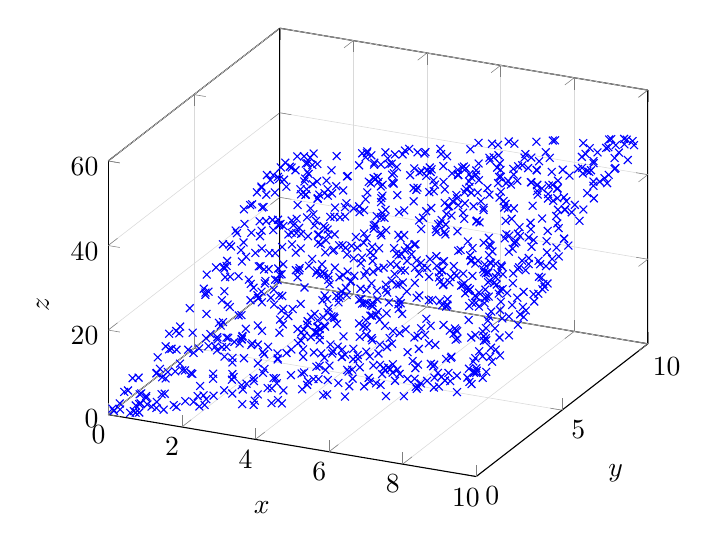
\begin{tikzpicture}
	\begin{axis}[
	xmin=0,xmax=10,xlabel=$x$,
	ymin=0,ymax=10,ylabel=$y$,
	zmin=0,zmax=60,zlabel=$z$,
	grid=both,
	grid style={line width=.2pt, draw=gray!30},
	%ytick={0,0.2,0.4,0.6,0.8,1},
	%ztick={0,0.2,0.4,0.6,0.8,1},
	]
	\addplot3[mark=x,only marks, blue] coordinates {
		(8.30,1.14,20.01)
		(8.49,7.96,40.87)
		(3.73,6.18,25.99)
		(5.93,0.70,13.97)
		(8.73,0.69,19.53)
		(9.34,1.36,22.75)
		(6.68,7.89,37.04)
		(2.07,0.92,6.91)
		(6.54,2.38,20.21)
		(0.72,2.44,8.75)
		(4.07,1.05,11.28)
		(6.67,8.58,39.09)
		(9.34,6.98,39.62)
		(8.11,7.34,38.23)
		(4.85,6.51,29.21)
		(7.57,5.16,30.62)
		(4.17,3.26,18.13)
		(9.72,6.62,39.29)
		(9.88,1.18,23.29)
		(8.64,1.48,21.72)
		(3.89,0.20,8.37)
		(4.55,9.64,38.02)
		(2.47,9.70,34.04)
		(7.84,1.24,19.40)
		(8.83,4.67,31.68)
		(9.14,6.57,37.98)
		(5.58,2.90,19.87)
		(5.99,7.55,34.61)
		(1.49,5.58,19.72)
		(9.00,4.28,30.83)
		(4.50,2.67,17.02)
		(2.06,7.54,26.73)
		(9.00,8.98,44.94)
		(7.63,7.28,37.11)
		(8.82,4.07,29.85)
		(2.85,9.38,33.85)
		(6.73,2.55,21.13)
		(6.64,5.33,29.28)
		(1.23,9.55,31.10)
		(4.07,2.68,16.18)
		(2.75,2.50,13.01)
		(7.17,9.28,42.16)
		(2.83,0.69,7.73)
		(8.96,2.99,26.91)
		(8.27,5.92,34.28)
		(3.90,2.03,13.90)
		(4.98,6.36,29.03)
		(6.95,7.98,37.85)
		(8.34,5.02,31.74)
		(6.10,6.51,31.72)
		(5.75,7.96,35.37)
		(3.26,2.33,13.52)
		(4.56,6.01,27.15)
		(7.14,1.12,17.65)
		(8.84,5.16,33.16)
		(7.21,8.38,39.55)
		(0.19,9.21,28.00)
		(6.75,4.98,28.44)
		(4.39,2.78,17.10)
		(4.38,6.53,28.33)
		(1.17,9.17,29.86)
		(8.15,5.10,31.59)
		(3.25,9.74,35.72)
		(2.46,1.97,10.84)
		(3.43,1.11,10.19)
		(3.76,2.97,16.43)
		(5.47,3.96,22.82)
		(5.62,4.21,23.86)
		(3.96,3.11,17.26)
		(3.98,6.94,28.78)
		(5.15,0.92,13.06)
		(6.58,4.02,25.21)
		(9.51,2.95,27.87)
		(7.22,3.06,23.64)
		(4.00,1.06,11.17)
		(8.32,5.94,34.45)
		(1.34,2.83,11.17)
		(0.60,1.55,5.87)
		(0.84,0.01,1.70)
		(1.64,2.84,11.79)
		(3.24,5.51,23.01)
		(3.02,8.71,32.16)
		(0.12,0.42,1.50)
		(5.40,9.05,37.94)
		(0.95,1.31,5.84)
		(1.47,8.34,27.94)
		(6.31,8.00,36.64)
		(8.59,9.18,44.72)
		(9.74,1.37,23.60)
		(5.71,5.05,26.56)
		(9.97,4.05,32.09)
		(5.54,1.74,16.28)
		(5.15,5.75,27.56)
		(3.31,6.06,24.80)
		(4.30,2.14,15.03)
		(4.92,5.20,25.43)
		(0.71,9.89,31.10)
		(8.88,4.90,32.45)
		(0.65,6.95,22.14)
		(4.36,4.11,21.07)
		(8.27,0.35,17.58)
		(3.95,2.93,16.68)
		(6.13,8.01,36.31)
		(8.19,3.47,26.77)
		(8.86,0.83,20.22)
		(9.31,5.11,33.96)
		(1.91,3.67,14.82)
		(2.59,7.39,27.36)
		(8.98,5.25,33.70)
		(5.93,8.05,36.00)
		(5.04,8.17,34.58)
		(6.13,1.89,17.94)
		(8.19,1.24,20.10)
		(5.32,8.21,35.27)
		(2.02,6.38,23.18)
		(4.54,0.16,9.56)
		(4.28,8.96,35.44)
		(9.66,5.15,34.78)
		(6.20,5.45,28.74)
		(6.95,6.06,32.10)
		(7.20,7.60,37.22)
		(3.47,8.55,32.60)
		(5.17,3.83,21.83)
		(5.57,0.85,13.67)
		(1.56,7.34,25.15)
		(5.62,3.32,21.20)
		(6.95,8.40,39.09)
		(4.26,3.72,19.68)
		(8.36,8.28,41.57)
		(7.31,1.77,19.92)
		(3.60,1.30,11.09)
		(4.54,8.80,35.48)
		(3.86,0.44,9.05)
		(7.76,6.87,36.11)
		(7.34,7.34,36.70)
		(4.30,4.37,21.72)
		(6.94,3.80,25.27)
		(9.45,9.80,48.29)
		(7.84,3.99,27.65)
		(7.06,4.40,27.32)
		(1.09,1.57,6.89)
		(3.90,3.26,17.58)
		(5.91,3.14,21.24)
		(4.59,8.95,36.02)
		(0.50,2.47,8.42)
		(2.29,3.11,13.89)
		(8.34,4.09,28.95)
		(0.16,7.08,21.55)
		(8.64,1.44,21.58)
		(0.78,8.71,27.70)
		(6.69,0.83,15.88)
		(5.00,4.62,23.86)
		(2.18,0.30,5.27)
		(5.72,7.53,34.03)
		(1.22,7.00,23.45)
		(6.71,2.15,19.86)
		(6.00,6.80,32.39)
		(0.56,5.57,17.84)
		(0.56,8.51,26.65)
		(1.53,5.59,19.81)
		(0.20,9.02,27.45)
		(4.35,4.20,21.29)
		(8.32,3.58,27.39)
		(6.17,4.89,27.02)
		(5.20,2.56,18.08)
		(8.64,9.29,45.15)
		(0.98,4.67,15.96)
		(9.08,2.54,25.78)
		(1.08,4.31,15.10)
		(5.17,7.03,31.42)
		(1.43,4.02,14.93)
		(5.59,1.82,16.64)
		(0.05,8.56,25.78)
		(7.67,5.84,32.86)
		(8.49,3.74,28.18)
		(9.17,2.22,24.99)
		(9.87,2.19,26.31)
		(5.05,5.22,25.77)
		(2.71,4.33,18.43)
		(1.01,7.41,24.25)
		(5.08,0.70,12.27)
		(5.86,8.47,37.13)
		(7.63,6.80,35.65)
		(0.83,1.37,5.76)
		(6.62,8.58,38.98)
		(5.17,2.00,16.33)
		(1.71,6.07,21.64)
		(9.39,5.43,35.06)
		(5.90,1.62,16.68)
		(4.41,0.06,8.98)
		(9.42,7.71,41.98)
		(6.56,7.65,36.06)
		(4.52,4.21,21.67)
		(8.40,0.57,18.50)
		(5.33,5.86,28.22)
		(5.54,1.74,16.30)
		(6.80,7.29,35.46)
		(3.67,5.34,23.37)
		(2.39,2.53,12.38)
		(5.79,9.17,39.09)
		(8.67,7.58,40.08)
		(4.07,8.87,34.75)
		(1.13,0.69,4.32)
		(4.44,1.84,14.38)
		(3.00,7.37,28.12)
		(4.01,6.97,28.93)
		(8.33,7.77,39.98)
		(4.04,5.02,23.13)
		(3.90,4.25,20.57)
		(3.60,6.11,25.55)
		(1.40,8.56,28.48)
		(2.60,6.71,25.33)
		(0.87,5.24,17.44)
		(4.29,2.99,17.55)
		(2.57,7.04,26.26)
		(2.98,3.82,17.40)
		(4.25,5.68,25.53)
		(1.19,8.88,29.02)
		(4.95,8.43,35.19)
		(7.06,8.99,41.09)
		(2.44,9.39,33.04)
		(7.85,8.15,40.16)
		(0.74,0.01,1.52)
		(3.94,0.03,7.97)
		(0.03,0.87,2.69)
		(2.21,2.61,12.24)
		(0.01,0.23,0.71)
		(1.89,4.24,16.51)
		(1.42,3.41,13.08)
		(2.68,5.41,21.60)
		(1.75,9.26,31.28)
		(1.39,2.98,11.73)
		(5.99,3.38,22.12)
		(9.01,8.59,43.81)
		(9.39,3.40,29.00)
		(2.21,1.38,8.57)
		(4.83,5.08,24.89)
		(3.76,8.57,33.22)
		(5.24,3.84,22.01)
		(2.65,6.96,26.17)
		(0.68,6.28,20.20)
		(4.36,4.50,22.24)
		(1.74,4.74,17.69)
		(0.26,9.50,29.01)
		(9.55,0.83,21.60)
		(4.31,2.80,17.01)
		(9.62,4.47,32.64)
		(7.62,5.88,32.88)
		(0.07,8.78,26.48)
		(6.80,4.69,27.67)
		(7.06,4.37,27.24)
		(6.45,7.46,35.29)
		(5.52,4.68,25.08)
		(2.18,8.61,30.19)
		(7.72,4.67,29.44)
		(2.28,4.98,19.50)
		(3.71,4.87,22.04)
		(8.91,2.29,24.70)
		(8.56,0.86,19.69)
		(4.02,0.67,10.07)
		(3.18,8.88,33.01)
		(6.09,2.33,19.17)
		(9.10,8.62,44.05)
		(9.09,7.12,39.53)
		(5.92,8.73,38.02)
		(3.33,9.38,34.79)
		(8.53,1.40,21.25)
		(4.42,3.94,20.66)
		(9.04,9.81,47.50)
		(0.33,6.45,20.01)
		(5.32,8.96,37.54)
		(7.16,4.82,28.80)
		(1.79,0.14,4.01)
		(3.37,6.23,25.42)
		(1.88,2.31,10.69)
		(3.22,5.27,22.26)
		(4.04,7.25,29.83)
		(5.49,6.07,29.19)
		(0.49,5.88,18.63)
		(5.53,4.33,24.06)
		(2.75,2.44,12.82)
		(2.42,4.29,17.70)
		(2.43,0.10,5.17)
		(1.54,6.09,21.35)
		(9.56,9.58,47.87)
		(9.36,0.95,21.58)
		(8.19,0.36,17.44)
		(7.28,8.86,41.15)
		(1.76,2.47,10.92)
		(3.60,0.09,7.47)
		(1.89,8.15,28.22)
		(0.01,1.40,4.24)
		(3.16,8.80,32.72)
		(7.00,0.95,16.85)
		(6.25,3.53,23.08)
		(5.43,5.93,28.66)
		(4.39,5.85,26.34)
		(2.87,6.68,25.78)
		(5.02,6.48,29.47)
		(7.62,4.33,28.23)
		(7.62,1.40,19.44)
		(5.76,7.52,34.08)
		(7.48,2.42,22.21)
		(6.46,6.50,32.42)
		(1.23,8.57,28.19)
		(5.04,0.84,12.62)
		(3.47,9.72,36.11)
		(0.92,0.31,2.79)
		(1.48,8.35,28.02)
		(1.98,8.36,29.03)
		(6.72,0.50,14.94)
		(4.32,5.46,25.01)
		(6.94,9.43,42.18)
		(2.57,3.21,14.78)
		(0.10,8.06,24.39)
		(5.32,6.01,28.69)
		(2.79,7.90,29.28)
		(9.46,7.99,42.90)
		(9.06,0.50,19.62)
		(3.93,2.83,16.35)
		(0.25,6.53,20.10)
		(6.71,4.90,28.12)
		(8.37,9.73,45.93)
		(9.71,7.48,41.88)
		(0.57,5.68,18.17)
		(4.50,2.99,17.98)
		(5.82,2.56,19.33)
		(6.87,8.87,40.33)
		(7.19,4.47,27.79)
		(6.50,8.16,37.48)
		(7.27,0.98,17.49)
		(3.74,8.60,33.26)
		(5.82,0.28,12.46)
		(1.16,8.99,29.30)
		(0.58,9.00,28.15)
		(9.80,5.24,35.32)
		(2.85,1.20,9.30)
		(5.95,1.78,17.23)
		(9.62,7.06,40.43)
		(1.86,8.31,28.66)
		(1.93,0.35,4.91)
		(3.42,7.58,29.57)
		(9.33,9.57,47.37)
		(3.91,3.43,18.10)
		(2.73,6.38,24.61)
		(1.52,3.43,13.33)
		(3.97,2.16,14.44)
		(3.75,7.86,31.08)
		(1.31,7.23,24.31)
		(4.35,2.79,17.07)
		(0.92,5.82,19.30)
		(6.15,4.21,24.92)
		(0.11,0.92,2.98)
		(5.73,0.24,12.19)
		(7.90,4.91,30.53)
		(2.35,2.78,13.06)
		(4.48,3.40,19.15)
		(5.69,2.87,20.01)
		(0.61,1.71,6.36)
		(4.96,3.99,21.90)
		(6.42,6.98,33.78)
		(2.21,2.04,10.54)
		(8.37,6.66,36.73)
		(9.71,4.43,32.71)
		(8.46,4.33,29.93)
		(5.06,1.75,15.38)
		(2.79,1.93,11.37)
		(7.47,6.16,33.42)
		(2.37,2.69,12.81)
		(9.57,5.60,35.94)
		(6.20,9.45,40.75)
		(6.00,7.14,33.44)
		(1.73,6.79,23.83)
		(0.90,9.59,30.59)
		(2.55,7.75,28.37)
		(8.59,6.08,35.40)
		(9.11,9.48,46.66)
		(7.00,0.60,15.78)
		(7.25,2.69,22.57)
		(2.30,9.87,34.20)
		(5.76,7.72,34.69)
		(8.11,4.75,30.47)
		(4.04,6.81,28.50)
		(9.88,4.17,32.28)
		(0.90,3.80,13.20)
		(3.21,2.13,12.82)
		(5.11,3.83,21.72)
		(0.61,0.30,2.10)
		(7.26,4.72,28.68)
		(5.57,3.33,21.13)
		(5.29,9.76,39.86)
		(8.30,5.55,33.26)
		(8.59,8.46,42.56)
		(7.89,4.08,28.02)
		(3.18,4.62,20.22)
		(4.52,8.26,33.83)
		(7.52,9.91,44.78)
		(1.10,5.24,17.92)
		(1.10,9.25,29.96)
		(2.70,7.39,27.57)
		(5.25,5.67,27.52)
		(9.73,9.69,48.52)
		(7.10,8.24,38.94)
		(3.12,9.60,35.03)
		(2.91,6.46,25.22)
		(8.50,3.80,28.39)
		(9.12,4.77,32.53)
		(6.39,9.12,40.14)
		(2.55,0.15,5.55)
		(0.89,1.57,6.47)
		(8.38,4.72,30.91)
		(5.85,5.43,27.98)
		(9.48,0.60,20.75)
		(0.61,6.58,20.96)
		(5.85,8.90,38.38)
		(2.85,1.10,8.99)
		(8.28,4.38,29.69)
		(1.91,2.80,12.23)
		(4.43,9.85,38.41)
		(3.93,6.09,26.13)
		(8.27,2.54,24.14)
		(6.77,1.33,17.52)
		(2.08,5.45,20.50)
		(3.18,8.28,31.20)
		(1.34,8.37,27.79)
		(6.71,8.33,38.43)
		(5.71,2.04,17.53)
		(1.70,5.44,19.73)
		(1.48,8.75,29.20)
		(4.76,1.21,13.15)
		(9.08,8.56,43.85)
		(5.52,9.00,38.04)
		(0.33,2.18,7.19)
		(0.54,0.77,3.39)
		(8.05,4.74,30.33)
		(4.51,8.35,34.08)
		(3.83,4.69,21.73)
		(7.90,4.14,28.21)
		(3.64,5.03,22.37)
		(5.32,1.25,14.41)
		(7.12,1.32,18.20)
		(8.71,8.70,43.54)
		(3.29,6.03,24.66)
		(6.50,2.65,20.96)
		(9.75,8.65,45.44)
		(0.76,0.58,3.26)
		(5.87,4.58,25.47)
		(4.14,7.22,29.94)
		(3.09,3.39,16.35)
		(2.64,4.01,17.31)
		(7.59,5.27,30.98)
		(9.95,8.94,46.73)
		(1.87,7.78,27.08)
		(7.81,0.69,17.70)
		(1.96,2.79,12.28)
		(9.92,3.79,31.23)
		(8.02,8.65,41.99)
		(4.24,4.20,21.08)
		(7.29,2.40,21.77)
		(4.98,5.98,27.90)
		(8.09,4.79,30.56)
		(3.57,8.99,34.09)
		(0.73,9.35,29.51)
		(5.91,8.18,36.36)
		(9.10,7.09,39.47)
		(1.94,7.43,26.17)
		(4.32,9.00,35.64)
		(7.49,0.65,16.94)
		(0.39,3.36,10.86)
		(9.46,0.04,19.06)
		(7.64,8.28,40.12)
		(5.59,5.07,26.40)
		(1.84,3.66,14.66)
		(4.98,2.27,16.76)
		(5.18,5.35,26.40)
		(9.94,2.89,28.57)
		(8.55,0.68,19.15)
		(9.62,0.85,21.80)
		(6.79,0.68,15.63)
		(4.04,4.10,20.36)
		(9.35,1.23,22.40)
		(4.79,4.43,22.88)
		(2.32,8.99,31.60)
		(3.96,3.54,18.53)
		(7.05,1.20,17.71)
		(5.59,5.69,28.24)
		(7.57,8.75,41.38)
		(9.95,3.49,30.37)
		(9.62,0.42,20.51)
		(5.35,1.42,14.97)
		(9.64,0.77,21.58)
		(1.16,7.41,24.53)
		(0.51,4.57,14.72)
		(3.04,6.68,26.13)
		(5.80,6.99,32.58)
		(5.31,5.71,27.76)
		(9.01,6.29,36.88)
		(5.41,8.78,37.14)
		(4.32,6.62,28.51)
		(5.43,8.75,37.12)
		(7.12,4.68,28.27)
		(0.17,1.41,4.57)
		(8.01,0.68,18.06)
		(1.43,7.14,24.28)
		(4.78,3.08,18.81)
		(2.57,6.71,25.27)
		(3.69,6.52,26.95)
		(6.62,5.31,29.17)
		(1.70,7.15,24.85)
		(2.79,5.05,20.72)
		(1.98,4.88,18.60)
		(1.95,4.98,18.84)
		(3.27,9.36,34.62)
		(8.80,3.89,29.29)
		(4.71,1.17,12.94)
		(4.04,2.40,15.29)
		(1.79,6.85,24.13)
		(9.69,8.39,44.56)
		(4.07,9.70,37.25)
		(8.44,2.15,23.34)
		(6.15,7.60,35.12)
		(3.77,5.84,25.06)
		(8.77,4.03,29.63)
		(7.85,5.10,31.00)
		(4.65,4.96,24.17)
		(8.14,6.51,35.82)
		(8.98,7.44,40.28)
		(4.29,3.02,17.64)
		(3.34,0.90,9.37)
		(5.97,8.26,36.71)
		(9.02,3.90,29.73)
		(7.02,7.75,37.30)
		(3.77,1.79,12.93)
		(7.35,1.09,17.98)
		(9.54,9.05,46.24)
		(5.43,8.76,37.15)
		(5.40,10.00,40.80)
		(3.11,8.64,32.15)
		(0.71,0.37,2.53)
		(1.82,5.45,19.98)
		(0.93,9.98,31.79)
		(4.63,5.11,24.60)
		(0.09,8.74,26.39)
		(9.15,0.70,20.41)
		(6.43,9.88,42.48)
		(0.01,9.23,27.71)
		(0.30,5.64,17.54)
		(2.08,4.31,17.11)
		(4.55,3.38,19.23)
		(1.27,7.21,24.17)
		(0.09,0.14,0.58)
		(7.27,3.74,25.76)
		(3.54,9.23,34.76)
		(7.80,5.46,32.00)
		(4.37,4.74,22.95)
		(4.37,4.97,23.63)
		(0.49,3.09,10.25)
		(0.50,9.51,29.52)
		(0.91,9.82,31.28)
		(5.94,5.14,27.29)
		(2.41,9.93,34.60)
		(8.41,4.56,30.50)
		(8.57,4.26,29.93)
		(9.64,2.13,25.67)
		(4.89,1.93,15.58)
		(2.20,8.33,29.39)
		(2.26,7.27,26.32)
		(5.37,5.30,26.63)
		(7.62,8.29,40.11)
		(3.48,5.12,22.31)
		(4.61,5.52,25.78)
		(6.39,2.13,19.19)
		(9.17,5.88,35.98)
		(1.62,1.43,7.51)
		(7.16,0.52,15.88)
		(5.78,6.83,32.05)
		(4.33,6.09,26.92)
		(8.84,2.20,24.27)
		(3.93,4.06,20.05)
		(1.79,6.30,22.48)
		(6.33,5.55,29.33)
		(6.24,1.28,16.31)
		(3.28,1.69,11.63)
		(8.03,0.01,16.09)
		(9.99,4.18,32.53)
		(9.81,4.88,34.27)
		(1.27,1.60,7.34)
		(2.32,6.67,24.65)
		(0.24,0.18,1.01)
		(6.07,1.20,15.74)
		(1.11,9.52,30.78)
		(4.07,9.76,37.42)
		(8.84,0.31,18.61)
		(5.48,4.94,25.78)
		(3.69,8.63,33.26)
		(2.08,2.43,11.45)
		(4.41,8.34,33.85)
		(9.56,8.14,43.53)
		(1.24,6.29,21.35)
		(4.71,0.02,9.48)
		(8.57,3.80,28.53)
		(0.43,9.04,28.00)
		(6.92,6.80,34.24)
		(9.79,3.79,30.94)
		(2.83,6.32,24.62)
		(1.34,2.43,9.97)
		(6.85,5.71,30.85)
		(9.09,9.82,47.64)
		(6.11,8.50,37.71)
		(9.00,2.83,26.50)
		(1.93,6.82,24.34)
		(7.54,3.58,25.83)
		(3.46,9.87,36.53)
		(4.19,0.84,10.89)
		(1.56,2.50,10.62)
		(8.19,8.11,40.72)
		(6.25,0.84,15.03)
		(7.39,5.31,30.71)
		(8.05,8.01,40.12)
		(0.67,7.39,23.51)
		(9.51,1.42,23.27)
		(4.98,4.38,23.09)
		(7.55,3.50,25.61)
		(7.42,4.78,29.20)
		(8.31,5.87,34.24)
		(1.57,1.46,7.50)
		(4.57,9.05,36.31)
		(6.18,6.40,31.57)
		(9.32,1.63,23.53)
		(8.35,5.66,33.68)
		(8.95,9.32,45.86)
		(5.83,7.83,35.14)
		(5.83,6.86,32.23)
		(8.55,4.66,31.09)
		(0.35,2.60,8.51)
		(8.85,5.69,34.79)
		(4.08,2.49,15.62)
		(0.36,3.19,10.31)
		(7.46,9.11,42.25)
		(1.55,8.85,29.65)
		(1.44,7.95,26.72)
		(6.06,9.26,39.89)
		(2.54,1.79,10.45)
		(3.24,5.18,22.01)
		(4.02,6.27,26.85)
		(4.06,9.13,35.52)
		(3.86,6.64,27.64)
		(6.10,3.89,23.87)
		(1.67,7.40,25.54)
		(1.88,8.18,28.29)
		(0.95,6.00,19.90)
		(3.23,0.85,9.01)
		(7.70,9.22,43.06)
		(2.34,0.54,6.29)
		(7.40,5.27,30.62)
		(6.93,1.19,17.42)
		(8.24,3.80,27.89)
		(8.28,8.13,40.94)
		(2.93,2.44,13.19)
		(3.09,8.84,32.72)
		(5.23,7.13,31.84)
		(3.25,3.78,17.85)
		(8.32,2.49,24.10)
		(8.10,2.53,23.79)
		(5.57,7.67,34.16)
		(2.63,0.50,6.76)
		(6.81,6.85,34.17)
		(2.34,6.20,23.28)
		(4.56,7.47,31.53)
		(3.85,9.77,37.01)
		(5.39,3.84,22.29)
		(9.92,2.60,27.64)
		(7.55,8.77,41.43)
		(9.80,8.06,43.79)
		(2.35,4.61,18.53)
		(5.29,0.91,13.30)
		(0.51,5.64,17.96)
		(7.57,1.87,20.76)
		(6.02,5.32,27.99)
		(8.57,3.55,27.79)
		(9.88,3.15,29.21)
		(9.29,7.27,40.39)
		(4.10,5.16,23.66)
		(0.00,7.91,23.73)
		(5.41,2.04,16.95)
		(2.08,6.78,24.50)
		(2.19,0.52,5.96)
		(3.26,8.01,30.55)
		(0.96,6.79,22.28)
		(7.48,9.46,43.33)
		(7.49,0.92,17.72)
		(5.43,9.08,38.12)
		(3.38,5.10,22.06)
		(8.32,6.15,35.09)
		(5.53,3.16,20.53)
		(9.58,0.77,21.48)
		(8.93,8.51,43.38)
		(3.57,1.45,11.47)
		(5.46,3.70,22.04)
		(3.47,6.22,25.61)
		(6.23,9.98,42.38)
		(7.97,5.17,31.45)
		(7.46,9.91,44.63)
		(1.26,2.27,9.31)
		(8.22,3.98,28.39)
		(0.25,6.97,21.40)
		(4.14,0.65,10.23)
		(7.31,7.48,37.06)
		(7.81,4.20,28.24)
		(3.67,8.11,31.69)
		(7.45,3.80,26.29)
		(8.92,3.19,27.42)
		(2.43,9.86,34.43)
		(1.30,7.18,24.14)
		(2.25,4.13,16.90)
		(3.50,0.99,9.96)
		(2.87,7.35,27.78)
		(9.27,6.37,37.67)
		(0.51,0.74,3.24)
		(5.93,1.21,15.47)
		(1.63,9.82,32.71)
		(8.38,4.97,31.67)
		(1.68,0.22,4.02)
		(5.02,0.54,11.66)
		(9.99,1.41,24.21)
		(3.55,8.93,33.91)
		(0.47,4.66,14.92)
		(2.14,5.61,21.10)
		(3.98,4.94,22.79)
		(3.34,0.68,8.71)
		(2.30,8.98,31.52)
		(9.36,2.89,27.38)
		(6.83,2.69,21.74)
		(9.62,5.94,37.07)
		(4.38,4.76,23.04)
		(9.40,3.68,29.86)
		(0.06,6.56,19.79)
		(6.10,9.38,40.35)
		(8.01,6.20,34.63)
		(2.33,2.83,13.14)
		(9.32,2.05,24.80)
		(7.63,4.39,28.44)
		(8.26,0.27,17.35)
		(5.73,8.76,37.75)
		(7.93,6.10,34.15)
		(3.29,2.04,12.69)
		(2.23,5.20,20.07)
		(3.12,0.54,7.86)
		(5.85,8.62,37.56)
		(8.30,4.43,29.89)
		(2.90,5.48,22.25)
		(4.03,5.67,25.06)
		(8.62,6.80,37.65)
		(6.15,3.71,23.44)
		(9.91,0.78,22.17)
		(2.04,4.56,17.76)
		(8.27,0.48,17.98)
		(6.76,7.38,35.66)
		(2.49,0.38,6.12)
		(4.76,9.54,38.14)
		(3.99,7.42,30.25)
		(5.99,9.37,40.11)
		(8.01,5.13,31.41)
		(1.05,2.41,9.33)
		(8.21,2.60,24.23)
		(8.41,7.59,39.59)
		(3.55,9.93,36.89)
		(4.30,3.57,19.30)
		(5.72,7.53,34.03)
		(7.01,1.10,17.32)
		(7.42,5.97,32.76)
		(7.58,4.31,28.08)
		(3.89,7.31,29.70)
		(4.29,2.61,16.42)
		(9.56,0.95,21.97)
		(5.73,4.51,24.99)
		(8.50,6.40,36.20)
		(2.76,1.32,9.49)
		(6.22,4.53,26.03)
		(5.88,6.52,31.33)
		(9.63,8.27,44.08)
		(0.86,3.08,10.96)
		(5.00,4.02,22.08)
		(5.22,8.84,36.96)
		(0.90,7.01,22.82)
		(9.05,2.42,25.35)
		(8.84,7.60,40.48)
		(4.39,2.91,17.51)
		(7.82,2.77,23.96)
		(1.48,0.06,3.15)
		(6.20,3.75,23.64)
		(2.61,4.37,18.32)
		(4.46,3.04,18.04)
		(8.44,2.91,25.61)
		(1.96,2.43,11.20)
		(3.04,9.37,34.18)
		(4.83,8.60,35.47)
		(3.38,3.97,18.67)
		(7.98,4.79,30.35)
		(9.87,5.65,36.70)
		(1.59,4.90,17.87)
		(2.37,2.70,12.83)
		(7.02,9.90,43.74)
		(3.75,1.84,13.02)
		(9.74,8.62,45.32)
		(9.72,0.33,20.43)
		(6.44,3.32,22.83)
		(8.60,7.49,39.66)
		(4.02,6.44,27.37)
		(6.32,1.69,17.72)
		(9.85,9.52,48.27)
		(5.59,5.43,27.49)
		(9.34,2.51,26.21)
		(7.20,5.79,31.76)
		(4.84,9.15,37.15)
		(6.39,8.96,39.65)
		(8.88,4.83,32.23)
		(1.99,4.43,17.26)
		(3.95,3.12,17.26)
		(9.92,0.55,21.50)
		(4.02,7.54,30.66)
		(6.59,1.32,17.14)
		(9.01,3.56,28.70)
		(9.95,3.96,31.78)
		(6.53,8.86,39.63)
		(1.08,0.21,2.81)
		(0.36,8.44,26.04)
		(6.18,2.88,21.00)
		(5.67,2.50,18.85)
		(9.62,4.88,33.89)
		(7.46,7.29,36.79)
		(6.63,2.03,19.33)
		(5.23,2.16,16.95)
		(2.60,9.76,34.49)
		(9.62,5.93,37.04)
		(5.40,3.04,19.94)
		(0.30,9.68,29.64)
		(6.96,8.96,40.81)
		(5.20,1.90,16.10)
		(0.59,0.02,1.23)
		(8.90,7.12,39.15)
		(3.30,8.68,32.64)
		(2.30,1.18,8.14)
		(1.14,0.39,3.45)
		(3.11,5.98,24.16)
		(2.28,6.04,22.70)
		(6.52,5.16,28.53)
		(0.66,0.08,1.55)
		(2.75,6.89,26.18)
		(2.82,9.46,34.02)
		(8.80,8.74,43.81)
		(4.44,1.13,12.28)
		(7.56,3.55,25.76)
		(6.03,2.42,19.32)
		(7.83,5.60,32.48)
		(1.14,6.13,20.66)
		(9.79,3.01,28.60)
		(8.49,7.98,40.92)
		(0.51,7.96,24.88)
		(4.66,7.81,32.76)
		(3.26,3.51,17.05)
		(6.30,0.54,14.23)
		(2.30,7.09,25.87)
		(5.80,9.93,41.39)
		(6.03,1.62,16.94)
		(6.00,1.14,15.40)
		(4.48,9.13,36.35)
		(0.35,4.82,15.16)
		(5.14,8.52,35.83)
		(4.08,8.10,32.45)
		(1.08,1.87,7.76)
		(4.60,2.47,16.61)
		(4.51,0.54,10.64)
		(5.51,6.09,29.29)
		(8.05,7.77,39.43)
		(7.01,5.11,29.35)
		(8.72,0.28,18.28)
		(0.52,9.90,30.76)
		(2.20,5.01,19.42)
		(4.60,3.32,19.15)
		(9.59,1.74,24.39)
		(7.90,6.26,34.57)
		(4.52,5.75,26.29)
		(3.33,7.51,29.20)
		(0.59,1.54,5.79)
		(7.41,3.57,25.52)
		(5.07,1.44,14.45)
		(2.00,8.51,29.52)
		(4.27,3.38,18.68)
		(1.69,2.75,11.63)
		(7.52,0.06,15.21)
		(3.68,8.02,31.42)
		(9.42,4.97,33.76)
		(0.17,5.38,16.48)
		(8.29,8.71,42.71)
		(6.27,7.23,34.22)
		(5.39,6.68,30.82)
		(6.51,1.79,18.37)
		(7.27,5.50,31.05)
		(0.94,9.60,30.69)
		(8.78,5.96,35.43)
		(0.14,8.09,24.54)
		(2.94,9.85,35.42)
		(1.80,8.86,30.18)
		(9.26,2.14,24.94)
		(0.68,0.35,2.40)
		(5.81,4.51,25.16)
		(6.37,0.14,13.16)
		(6.51,4.74,27.24)
		(8.65,9.51,45.83)
		(0.56,2.49,8.59)
		(8.17,3.86,27.93)
		(5.29,4.31,23.52)
		(6.94,8.31,38.81)
		(2.12,8.25,28.99)
		(5.43,4.53,24.46)
		(7.03,3.81,25.47)
		(9.56,9.26,46.90)
		(4.45,7.41,31.12)
		(0.85,7.38,23.84)
		(0.57,9.47,29.55)
		(6.29,5.10,27.89)
		(7.96,7.92,39.68)
		(6.91,4.52,27.39)
		(3.45,8.49,32.38)
		(9.47,3.90,30.65)
		(5.20,7.38,32.56)
		(9.54,9.76,48.37)
		(0.74,5.23,17.17)
		(2.07,4.30,17.04)
		(7.75,2.07,21.72)
		(9.14,3.23,27.99)
		(7.83,1.11,18.98)
		(2.96,3.75,17.17)
		(1.52,3.30,12.93)
		(8.48,3.42,27.22)
		(7.85,8.17,40.21)
		(2.71,5.32,21.37)
		(2.28,5.21,20.19)
		(3.21,7.74,29.65)
		(8.30,1.20,20.20)
		(8.22,6.25,35.21)
		(5.71,3.47,21.81)
		(5.72,3.35,21.48)
		(2.86,5.75,22.96)
		(6.99,8.64,39.90)
		(7.96,1.99,21.88)
		(4.42,6.72,29.01)
		(4.46,9.02,35.98)
		(4.66,1.99,15.29)
		(2.79,2.98,14.53)
		(6.75,4.97,28.40)
		(9.04,8.90,44.77)
		(9.09,5.01,33.21)
		(7.47,2.77,23.25)
		(2.61,5.34,21.23)
		(6.90,5.74,31.02)
		(1.32,4.13,15.02)
		(1.24,0.15,2.91)
		(1.91,7.03,24.90)
		(1.46,5.07,18.12)
		(5.85,3.81,23.14)
		(0.73,0.65,3.42)
		(8.22,3.59,27.20)
		(7.23,2.34,21.49)
		(9.26,2.04,24.62)
		(4.93,8.14,34.27)
		(6.55,3.93,24.90)
		(8.90,0.54,19.41)
		(5.39,3.75,22.02)
		(2.82,7.75,28.89)
		(9.76,1.65,24.48)
		(0.36,9.12,28.10)
		(3.26,3.19,16.10)
		(9.73,3.30,29.35)
		(3.65,2.04,13.43)
		(3.09,7.67,29.20)
		(1.21,0.70,4.52)
		(9.16,9.50,46.82)
		(1.35,1.58,7.46)
		(3.32,2.86,15.24)
		(8.97,6.87,38.56)
		(5.00,1.41,14.23)
		(6.15,5.12,27.67)
		(5.83,7.21,33.30)
		(6.98,9.29,41.83)
		(0.29,7.32,22.55)
		(5.28,7.50,33.05)
		(0.32,4.07,12.86)
		(8.27,2.39,23.73)
		(3.40,5.21,22.43)
		(8.47,2.19,23.51)
		(2.46,8.42,30.19)
		(5.81,6.63,31.52)
		(9.38,8.16,43.24)
		(0.48,7.94,24.77)
		(0.54,4.69,15.15)
		(0.21,3.10,9.70)
		(6.81,6.88,34.26)
		(5.99,9.87,41.58)
	};
	\end{axis}
	\end{tikzpicture}
\end{center}

\subsection{Structure of multiple linear regression models}

Good news: simple linear models are a special case of \begriff{multiple linear regression} and with minor extensions everything we've looked at so far still applies. For $p$ predictors and data tuples $\{(x_{1i},x_{2i},...,x_{pi},Y_i)\mid i=1,...,n\}$, we assume the relationship
\begin{align}
	Y_i = \beta_0 + \sum_{j=1}^{p} \beta_jx_{ji} + \epsilon_i\notag
\end{align}
As before, we assume $\epsilon_i\overset{i.i.d}{\sim}Normal(0,\sigma)$. 

The matrix notation, $Y=X\beta + \epsilon$, now becomes very convenient:
\begin{align}
	Y = \begin{pmatrix}
		Y_1 \\ \vdots \\ Y_n
	\end{pmatrix}\quad X = \begin{pmatrix}
		1 & x_{11} & \dots & x_{p1} \\ \vdots & \vdots & \vdots & \vdots \\ 1 & x_{1n} & \dots &  x_{pn}
	\end{pmatrix} \quad \beta = \begin{pmatrix}
		\beta_0 \\ \vdots \\ \beta_p
	\end{pmatrix}\quad \epsilon = \begin{pmatrix}
		\epsilon_1 \\ \vdots \\ \epsilon_n
	\end{pmatrix} \notag
\end{align}

As before, the random variable notation is
\begin{align}
	Y_i &\overset{i.i.d}{\sim} Normal\left(\beta_0 + \sum_{j=1}^{p} \beta_jx_{ji},\sigma\right) \notag \\
	Y &\sim Normal(X\beta,\mathbbm{1}\sigma) \notag
\end{align}

Model fitting using Maximum Likelihood Estimation (MLE) proceeds in the same way as for simple linear models seen before and is equivalent to Ordinary Least Squares (OLS) fitting. The likelihood function is given by
\begin{align}
	L(\beta\mid X) = \prod_{i=1}^n f_{Normal}\left(Y_i,\mu=\beta_0+\sum_{j=1}^{p} \beta_jx_{ji},\sigma\right)\notag
\end{align}
where $f_{Normal}$ is the PDF for the normal distribution evaluated at $Y_i$. The exact equations for parameter MLEs are
\begin{align}
	\label{MLR_parameter_estimates}
	\begin{split}
		\hat{\beta} &= (X^TX)^{-1}X^TY \\
		\hat{\sigma}^2 &= \frac{1}{n-(p+1)}(Y-X\hat{\beta})^T(Y-X\hat{\beta})
	\end{split}
\end{align}
Fitted values for the response are: $\hat{Y} = X\hat{\beta}$. Parameter estimates for one explanatory variable describe the relationship between this variable and the response variable when all other explanatory variables are held fixed.

\subsection{Assumptions of linear models}

The assumptions for multiple linear regression models are the same as for simple linear models:
\begin{itemize}
	\item \textbf{Linearity:} response variable is a linear combination of the explanatory variables
	\item \textbf{Normality:} errors follow a normal distribution
	\item \textbf{Homoscedasticity:} variance of the response variable (or errors) is constant.
	\item \textbf{Independence:} the errors are uncorrelated (ideally statistically independent).
	\item \textbf{Weak exogeneity:} the explanatory variables can be treated as fixed values, rather than random variables.
\end{itemize}
However, there is one important addition:
\begin{itemize}
	\item \textbf{Lack of perfect multicollinearity:} if two explanatory variables are perfectly correlated, we can not solve the equation for parameter estimates (\cref{MLR_parameter_estimates}). Some (but not perfect!) correlation between explanatory variables my be permissible.
\end{itemize}

Model checking works in the same way as for simple linear models, using residuals. Additionally, may want to plot each explanatory variables versus residuals.

\subsection{Hypothesis testing on linear model parameters}

Using a conceptionally similar approach as for simple linear models, we can test hypothesis about the $\beta$s and construct confidence intervals for them. Importantly, the test statistics depend on the entries of the matrix
\begin{align}
	(X^TX)^{-1} = \begin{pmatrix}
		c_{00} & c_{01} & \dots & c_{0p} \\ \vdots & \vdots & \vdots & \vdots \\ c_{p0} & c_{p1} & \dots & c_{pp}
	\end{pmatrix}\notag
\end{align}
as $\sigma_{\hat{\beta_j}}=\hat{\sigma}\cdot\sqrt{c_{jj}}$ ($j=1,...,p$). Off-diagonal entries determine the covariance of estimates and are important for the variance in prediction. Generally, $\sigma$ needs to be estimated, so in practise we use \person{Student}'s t-distribution and the test statistic
\begin{align}
	t = \frac{\hat{\beta_j}-\text{hypothesised value}}{\hat{\sigma}\sqrt{c_{jj}}} \notag
\end{align}
\textcolor{red}{Many details omitted - software does the work for us!}

\subsection{Model selection}

With the more general Linear Model formulation, we can create many different models. How to choose which model to use?

\begin{example}
	Consider the range of electric vehicles.
	\begin{center}
		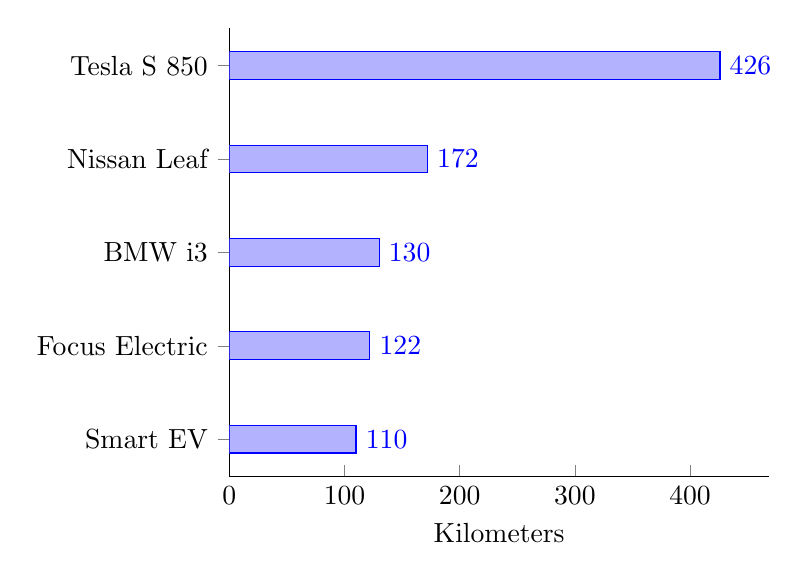
\begin{tikzpicture}
		\begin{axis}[ 
		xbar, xmin=0,
		xlabel={Kilometers},
		axis lines*=left,
		symbolic y coords={%
			{Smart EV},
			{Focus Electric},
			{BMW i3},
			{Nissan Leaf},
			{Tesla S 850}},
		ytick=data,
		nodes near coords, 
		nodes near coords align={horizontal},
		ytick=data,
		]
		\addplot coordinates {
			(110,{Smart EV}) 
			(122,{Focus Electric}) 
			(130,{BMW i3}) 
			(172,{Nissan Leaf})
			(426,{Tesla S 850})};
		\end{axis}
		\end{tikzpicture}
	\end{center}
	Depends on battery size, driving style or ambient temperature? Or all factors?
\end{example}

The right model depends on the purpose: Find all relevant factors? Prediction of range on a given day?

There is not one correct approach to model selection. What makes a good model depends on what it is designed for. Consequently, there are may different tools and techniques. Broadly, there are three types of model selection approaches:
\begin{itemize}
	\item Hypothesis tests on model parameters within models (include/exclude parameters).
	\item Measures that describe the quality or goodness of fit of models.
	\item Hypothesis tests comparing the fit of entire models (often related to measures from the previous point).
\end{itemize}
Fundamentally, model selection is at the heart of scientific inquiry. Statistical techniques offer one quantitative and rigorous approach. We'll go through a few of the most common statistical techniques.

\subsubsection{Hypothesis tests on model parameters}

We've encountered these already (test $H_0$: $\beta_j=0$). Could determine our model by fitting a full model that includes all conceivable explanatory variables first and than removing the explanatory variables for which we can't reject $H_0$.

\textbf{Problems:}
\begin{itemize}
	\item Multiple comparisons: conducting many hypothesis tests means that some may be rejected/accepted by chance (there are ways of dealing with this, e.g. \person{Bonferroni} correction).
	\item The model fit changes every time we remove an explanatory variable.
\end{itemize} 

While these tests are useful, we may want other approaches that allow us to test global hypotheses about models.

\subsubsection{$R^2$ and adjusted $R^2$}

Last lecture we looked at the \begriff{coefficient of correlation}, $R^2$ (proportion of variance in response explained by explanatory variables). Could use this to distinguish between models: the closer to 1 it is, the better the model.

\textbf{Problem:} $R^2$ always increases when we include more explanatory variables.

\begin{proposition}[\person{Occam}'s Razor by \person{William of Occam}, 1287-1347]
	\label{occams_razor}
	Entities are not to be multiplied without necessity (Latin: Non sunt multiplicanda entia sine necessitate.) Basically: prefer simpler models.
\end{proposition}

\textbf{Solution:} Adjusted $R^2$, $R^2_a$: unlike $R^2$, this takes into account the sample size $n$ and the number of model parameters.

\textbf{Warning:} I caution against relying on $R^2_a$ or $R^2$. They can only be usefully applied in particular circumstances.

\subsubsection{F-test on linear models}

Suppose we want to test a more general, global hypothesis about a linear model: \\
$H_0$: $\beta_1=\beta_2=\dots=\beta_p=0$ \\
$H_A$: At least one of the $\beta_j\neq 0$ \\
i.e. we compare our specified model to a constant model that only has an intercept $\beta_0$. This is called \begriff{F-test} or Analysis of Variance (Global). It uses the F-distribution and the test statistic can be expressed in terms of $R^2$ (we skip the details).

\textbf{Warnings}:
\begin{itemize}
	\item The test is very specific (we'll see a more general test in a moment). It asks if the improvement in model fit is larger than expected under $H_0$.
	\item It makes several assumptions (e.g. normally distributed errors), so check model assumptions hold.
	\item It doesn't tell us whether our model is correct.
\end{itemize}

\subsubsection{Quality measures based on the likelihood}

Techniques so far rely on the variance in the response explained by models. Recall the analogy for MLE of maximising $P(data\mid parameters)$. Could use the maximum likelihood of models, $\hat{L}$, to compare them: highest $\hat{L}$ indicates best model.

\textbf{Warning:} the likelihood faces the same problem as $R^2$ - it will always improve when more parameters are added to the model.

\textbf{Solution:} penalty for parameters in measures for relative model quality.
\begin{itemize}
	\item \textbf{Akaike Information Criterion:}
	\begin{align}
		\text{AIC} = 2k-2\ln(\hat{L})\notag
	\end{align}
	where $k$ is the number of model parameters, including the intercept, but typically excluding the error variance (as this is included in all models). Model with smallest AIC is best.
	\item \textbf{Bayesian Information Criterion:}
	\begin{align}
		\text{BIC} = \ln(n)k - 2\ln(\hat{L})\notag
	\end{align}
	Same idea, but penalty for parameters is stronger (based on different assumptions).
\end{itemize}

\textbf{Warning:} candidate models must be fitted to the same response data.

\subsubsection{Likelihood-ratio test for nested models}

The Likelihood-ratio test is a much more general version of the F-test. Consider a linear model, $M_1$ with parameters $\beta_{M_1}=\{\beta_1,\beta_2,...,\beta_p\}$. The test considers a restriction $M_0$ of $M_1$ where e.g. $\beta_{M_0} = \{\beta_1,\beta_2,...,\beta_q,0,...,0\}$ with $q<p$. We say $M_0$ is nested in $M_1$. We test the hypothesis: \\
$H_0$: $\beta = \beta_{M_0}$ \\
$H_A$: $\beta = \beta_{M_1}$ \\
using the test statistic 
\begin{align}
	D = 2\ln\left(\frac{\widehat{L_{M_1}}}{\widehat{L_{M_0}}}\right) = 2\bigg(\ln\big(\widehat{L_{M_1}}\big) - \ln\big(\widehat{L_{M_0}}\big)\bigg) \notag
\end{align}
Under some conditions and assuming $H_0$, $D$ is asymptotically distributed as $D\sim\chi^2_{p-q}$. This is a flexible and very useful test (e.g. tests on individual parameters). Also works when error distribution is not normal.

\subsection{Automated or standardised model selection strategies}

Model selection is time consuming. So people have tried to come up with standardised or even automated procedures, e.g. stepwise regression. Many software packages, including MATLAB, implement such procedures. There are many flavours, but the basic idea is:
\begin{enumerate}[label=\textbf{\arabic*.}]
	\item Identify response $Y$ and all potentially important explanatory variables $x_1,...,x_p$.
	\item Automatically work through models defined by all possible combinations of the $x_j$s, starting with simpler models.
	\item At each step use standard hypothesis tests (or other measures) to assess if additional explanatory variables improve model.
	\item Continue until some stopping criterion is reached.
\end{enumerate}

\textbf{Warning:} control of the process is relinquished to software that can be very intricate. Procedure conducts many statistical tests (multiple comparisons!). Because of these and other issues, many statisticians recommend not to use this approach.

\begin{center}
	\begin{tabular}{c|c}
		\textbf{use} & \textbf{technique} \\
		\hline
		Hypothesis tests for single parameters & t-test, Likelihood-ratio test \\
		Hypothesis tests for several parameters & F-test, Likelihood-ratio test \\
		Measures for relative quality of models & $R^2$, $R^2_a$, AIC, BIC
	\end{tabular}
\end{center}

\textbf{Warning}: none of these techniques tell you anything about the correctness of a model. So checking model assumptions separately is important!

Remember, none of these techniques are perfect. Choose your approach depending on what you are trying to achieve with your models. Within this in mind, prediction intervals and residual plots could be also used in model selection.
\pagebreak
\section{Model building}
So far, we have looked at linear models of the form
\begin{align}
	Y_i = \beta_0 + \beta_1x_{1i} + \beta_2x_{2i} + \dots + \beta_px_{pi} + \epsilon_i\notag
\end{align}
In this lecture, we extend this concept:
\begin{itemize}
	\item We look at how we can use different types of predictors to capture a wide range of relationships (e.g. capture non-linear relationship with linear model).
	\item We'll think about how to formulate models, depending on their use.
	\item We'll consider some common pitfalls in use of linear models.
\end{itemize}

\begin{example}
	Consider energy usage in houses, based on their size.
	\begin{center}
		\begin{tikzpicture}[scale=0.9]
			\begin{axis}[
				xmin=0, xmax=3, xlabel=$x$,
				ymin=4, ymax=8, ylabel=$y$,
				title=\textbf{Linear fit},
				axis x line=middle,
				axis y line=middle,
				samples=400
			]
			\addplot[blue, mark=x, only marks] coordinates	{
				(0.00,4.00)
				(0.10,4.42)
				(0.20,4.81)
				(0.30,5.18)
				(0.40,5.51)
				(0.50,5.82)
				(0.60,6.11)
				(0.70,6.37)
				(0.80,6.60)
				(0.90,6.81)
				(1.00,7.00)
				(1.10,7.17)
				(1.20,7.31)
				(1.30,7.43)
				(1.40,7.53)
				(1.50,7.61)
				(1.60,7.68)
				(1.70,7.72)
				(1.80,7.75)
				(1.90,7.75)
				(2.00,7.75)
				(2.10,7.72)
				(2.20,7.68)
				(2.30,7.63)
				(2.40,7.56)
				(2.50,7.48)
				(2.60,7.39)
				(2.70,7.28)
				(2.80,7.16)
				(2.90,7.03)
			};
			\addplot[mark=none] {0.96*x+5.4};
			\end{axis}
		\end{tikzpicture}
		\begin{tikzpicture}[scale=0.9]
		\begin{axis}[
		xmin=0, xmax=3, xlabel=$x$,
		ymin=4, ymax=8, ylabel=$y$,
		title=\textbf{Polynomial fit},
		axis x line=middle,
		axis y line=middle,
		samples=400
		]
		\addplot[blue, mark=x, only marks] coordinates	{
			(0.00,4.00)
			(0.10,4.42)
			(0.20,4.81)
			(0.30,5.18)
			(0.40,5.51)
			(0.50,5.82)
			(0.60,6.11)
			(0.70,6.37)
			(0.80,6.60)
			(0.90,6.81)
			(1.00,7.00)
			(1.10,7.17)
			(1.20,7.31)
			(1.30,7.43)
			(1.40,7.53)
			(1.50,7.61)
			(1.60,7.68)
			(1.70,7.72)
			(1.80,7.75)
			(1.90,7.75)
			(2.00,7.75)
			(2.10,7.72)
			(2.20,7.68)
			(2.30,7.63)
			(2.40,7.56)
			(2.50,7.48)
			(2.60,7.39)
			(2.70,7.28)
			(2.80,7.16)
			(2.90,7.03)
		};
		\addplot[mark=none] {0.1089*x^3-1.453*x^2+4.344*x+4};
		\end{axis}
		\end{tikzpicture}
	\end{center}
\end{example}

A simple linear models might tell us that a predictor is important, but it's no good prediction. Model building is a process that includes:
\begin{itemize}
	\item \textbf{Formulating a model:} model structure, we'll look at different types of predictors today.
	\item \textbf{Model fitting:} last two lectures
	\item \textbf{Model evaluation:} Check model assumptions hold, avoid common pitfalls
\end{itemize}

Before formulating a statistical model, it is good practice to explore the data. Look at scatter plots of predictors against the response and predictors against each other. Can help to develop an intuition for model structure. Look at distributions of response and predictors (e.g. look for outliers, can you capture the distribution with your model?) Think about what the model will be used for (e.g. prediction, or simply to find relevant explanatory variables).

\subsection{Types of predictors}

\subsubsection{qualitative vs quantitative}

So far, we have looked at \begriff{quantitative predictors} (numerical variables), e.g. temperature, energy usage, waiting time before computer processes data, ... But we can have \begriff{qualitative predictors} as well (categorical variables), e.g. type of engine, type fuel used, type of processor used, ... These are included in models using \begriff{dummy variables}.

\begin{example}
	Consider the performance $Y_i$ of diesel engines for three different fuel types A, B and C. We use the model $Y_i = \beta_0 + \beta_1x_{1i} + \beta_2x_{2i} + \epsilon_i$, where $x_{1i}$ and $x_{2i}$ are dummy variables such that
	\begin{align}
		x_{1i} &= \begin{cases}
		1 & \text{if fuel B is used} \\ 0 & \text{if not}
		\end{cases} \notag \\
		x_{2i} &= \begin{cases}
		1 & \text{if fuel C is used} \\ 0 & \text{if not}
		\end{cases} \notag 
	\end{align}
	The performance for fuel type A is captured in $\beta_0$.
\end{example}

Qualitative and quantitative predictors can be combined in models.

\begin{example}
	Consider fuel efficiency of car models from the 1950s (\textcolor{blue}{type 1}) and from the 1960s (\textcolor{red}{type 2}), depending on their weight. For car models $i=1,...,n$, we might consider the model $Y_i = \beta_0 + \beta_1x_i + \beta_2w_i + \epsilon_i$, where $Y_i$ is the efficiency in miles per gallon (MPG), $x_i$ is a dummy variable for the car type and $w_i$ is the weight of a car model. We might find:
	\begin{center}
	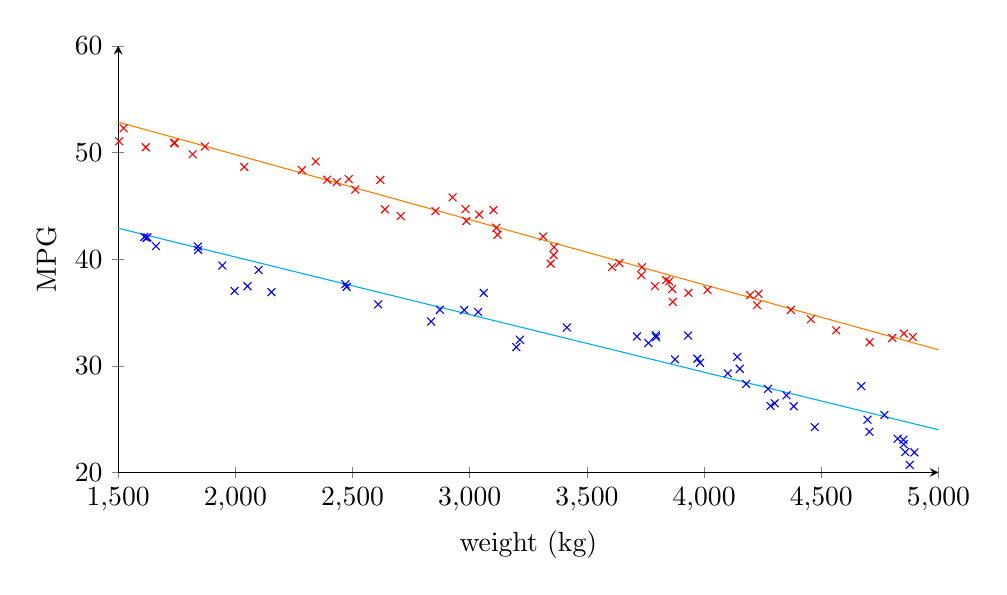
\begin{tikzpicture}
		\begin{axis}[
		xmin=1500, xmax=5000, xlabel=weight (kg),
		ymin=20, ymax=60, ylabel=MPG,
		axis x line=bottom,
		axis y line=left,
		samples = 400,
		height=7cm,
		width=12cm,
		domain=1500:5000
		]
		\addplot[blue, mark=x, only marks] coordinates {
			(1611.41,42.08)
			(1620.56,42.00)
			(1624.99,42.04)
			(1661.60,41.22)
			(1839.96,41.19)
			(1841.39,40.86)
			(1944.45,39.40)
			(1996.60,37.02)
			(2051.65,37.46)
			(2099.15,38.98)
			(2154.05,36.90)
			(2469.23,37.65)
			(2474.74,37.40)
			(2609.85,35.76)
			(2835.45,34.15)
			(2872.79,35.25)
			(2976.16,35.22)
			(3035.61,35.04)
			(3059.55,36.83)
			(3198.81,31.75)
			(3214.18,32.44)
			(3414.09,33.59)
			(3713.26,32.75)
			(3762.10,32.13)
			(3794.17,32.87)
			(3795.09,32.68)
			(3875.57,30.60)
			(3931.90,32.84)
			(3971.16,30.67)
			(3982.78,30.28)
			(4100.96,29.29)
			(4141.40,30.83)
			(4152.09,29.72)
			(4179.31,28.30)
			(4272.73,27.84)
			(4283.20,26.24)
			(4300.98,26.48)
			(4351.53,27.23)
			(4382.10,26.20)
			(4471.95,24.25)
			(4670.27,28.10)
			(4696.82,24.95)
			(4705.07,23.82)
			(4768.98,25.39)
			(4825.78,23.16)
			(4850.08,23.07)
			(4851.27,22.65)
			(4858.22,21.91)
			(4877.11,20.71)
			(4897.07,21.88)
		};
		\addplot[red,mark=x,only marks] coordinates {
			(1504.03,51.05)
			(1523.50,52.27)
			(1617.61,50.49)
			(1737.97,50.88)
			(1740.82,50.90)
			(1817.88,49.83)
			(1869.70,50.56)
			(2037.80,48.64)
			(2284.14,48.35)
			(2342.47,49.15)
			(2391.77,47.45)
			(2432.65,47.22)
			(2483.52,47.50)
			(2511.73,46.52)
			(2618.60,47.43)
			(2638.01,44.67)
			(2705.62,44.04)
			(2853.70,44.50)
			(2926.67,45.79)
			(2982.09,44.69)
			(2985.22,43.58)
			(3040.30,44.18)
			(3100.99,44.60)
			(3113.21,42.94)
			(3118.57,42.29)
			(3313.18,42.12)
			(3345.00,39.58)
			(3358.02,40.38)
			(3359.67,41.13)
			(3607.60,39.26)
			(3638.36,39.63)
			(3731.98,38.49)
			(3734.86,39.25)
			(3790.56,37.47)
			(3837.41,38.04)
			(3851.33,37.91)
			(3863.66,37.21)
			(3866.43,35.99)
			(3932.99,36.84)
			(4014.26,37.12)
			(4195.56,36.63)
			(4225.81,35.69)
			(4231.82,36.74)
			(4369.93,35.24)
			(4455.37,34.36)
			(4563.80,33.32)
			(4705.97,32.20)
			(4802.68,32.61)
			(4851.93,33.02)
			(4890.27,32.70)
		};
		\addplot[cyan,mark=none] {-0.0054*x+51};
		\addplot[orange,mark=none] {-0.0061*x+62};
		\end{axis}
	\end{tikzpicture}
\end{center}
\end{example}

\subsubsection{interaction terms}

So far, we have assumed that the effects of all explanatory variables are additive, e.g. as is $Y_i = \beta_0 + \beta_1x_{1i} + \beta_2x_{2i} + \epsilon_i$. What if the relationship between $Y_i$ and $x_{1i}$ depends on the value of $x_{2i}$? 

Then we need to consider \begriff{interaction terms} in our model, e.g. $Y_i = \beta_0 + \beta_1x_{1i} + \beta_2x_{2i} + \beta_3x_{1i}x_{2i} + \epsilon_i$. Interpretation of model parameters:
\begin{itemize}
	\item $(\beta_1 + \beta_3x_2)$ represents the change in $Y$ for every unit increase in $x_1$, holding $x_2$ fixed.
	\item $(\beta_2 + \beta_3x_1)$ represents the change in $Y$ for every unit increase in $x_2$, holding $x_1$ fixed.
	\item In model checking: if interaction term is important, then the interacting explanatory variable must be important and t-tests on them are meaningless.
\end{itemize}

This is still a linear model - the effects captured by parameters are additive.

\begin{example}
	Fuel efficiency $Y_i$ of car models from \textcolor{blue}{1970}, \textcolor{red}{'76} and \textcolor{green}{'82} depending on their weight $w_i$. Consider interaction between year built and weight.
	\begin{align}
		Y_i = \beta_0 + \beta_1x_{1i} + \beta_2x_{2i} + \beta_3w_i + \beta_4x_{1i}w_i + \beta_5x_{2i}w_i + \epsilon_i\notag
	\end{align}
	This model has main effects for year and weight and interaction terms. Model fitting:
	\begin{center}
	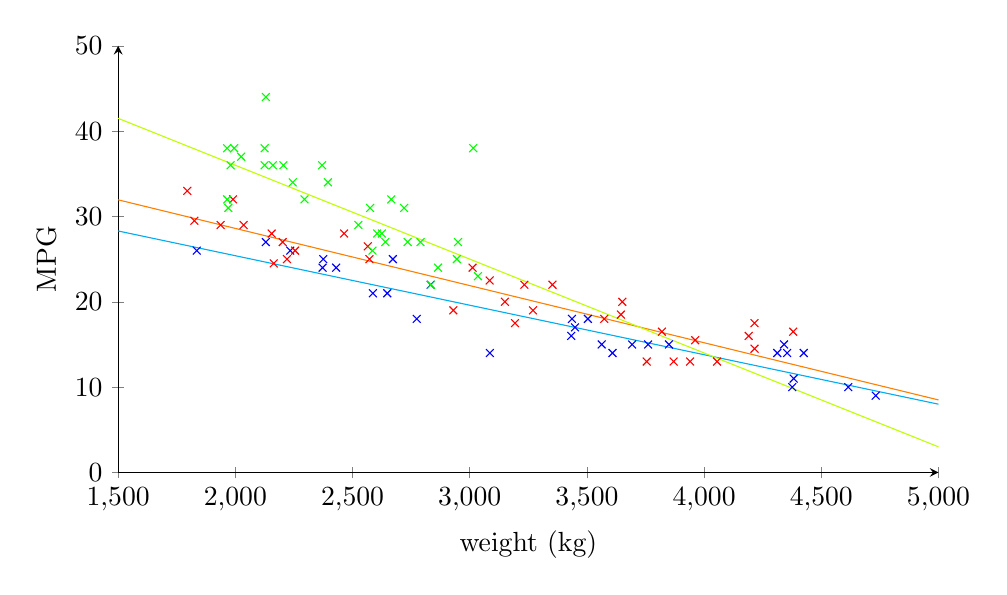
\begin{tikzpicture}
		\begin{axis}[
		xmin=1500, xmax=5000, xlabel=weight (kg),
		ymin=0, ymax=50, ylabel=MPG,
		axis x line=bottom,
		axis y line=left,
		samples = 400,
		height=7cm,
		width=12cm,
		domain=1500:5000
		]
		\addplot[blue, mark=x, only marks] coordinates {
			(3504.00,18.00)
			(3693.00,15.00)
			(3436.00,18.00)
			(3433.00,16.00)
			(3449.00,17.00)
			(4341.00,15.00)
			(4354.00,14.00)
			(4312.00,14.00)
			(4425.00,14.00)
			(3850.00,15.00)
			(3563.00,15.00)
			(3609.00,14.00)
			(3761.00,15.00)
			(3086.00,14.00)
			(2372.00,24.00)
			(2833.00,22.00)
			(2774.00,18.00)
			(2587.00,21.00)
			(2130.00,27.00)
			(1835.00,26.00)
			(2672.00,25.00)
			(2430.00,24.00)
			(2375.00,25.00)
			(2234.00,26.00)
			(2648.00,21.00)
			(4615.00,10.00)
			(4376.00,10.00)
			(4382.00,11.00)
			(4732.00,9.00)
		};
		\addplot[red,mark=x,only marks] coordinates {
			(2464.00,28.00)
			(2220.00,25.00)
			(2572.00,25.00)
			(2255.00,26.00)
			(2202.00,27.00)
			(4215.00,17.50)
			(4190.00,16.00)
			(3962.00,15.50)
			(4215.00,14.50)
			(3233.00,22.00)
			(3353.00,22.00)
			(3012.00,24.00)
			(3085.00,22.50)
			(2035.00,29.00)
			(2164.00,24.50)
			(1937.00,29.00)
			(1795.00,33.00)
			(3651.00,20.00)
			(3574.00,18.00)
			(3645.00,18.50)
			(3193.00,17.50)
			(1825.00,29.50)
			(1990.00,32.00)
			(2155.00,28.00)
			(2565.00,26.50)
			(3150.00,20.00)
			(3940.00,13.00)
			(3270.00,19.00)
			(2930.00,19.00)
			(3820.00,16.50)
			(4380.00,16.50)
			(4055.00,13.00)
			(3870.00,13.00)
			(3755.00,13.00)
		};
		\addplot[green,mark=x,only marks] coordinates {
			(2605.00,28.00)
			(2640.00,27.00)
			(2395.00,34.00)
			(2575.00,31.00)
			(2525.00,29.00)
			(2735.00,27.00)
			(2865.00,24.00)
			(3035.00,23.00)
			(1980.00,36.00)
			(2025.00,37.00)
			(1970.00,31.00)
			(2125.00,38.00)
			(2125.00,36.00)
			(2160.00,36.00)
			(2205.00,36.00)
			(2245.00,34.00)
			(1965.00,38.00)
			(1965.00,32.00)
			(1995.00,38.00)
			(2945.00,25.00)
			(3015.00,38.00)
			(2585.00,26.00)
			(2835.00,22.00)
			(2665.00,32.00)
			(2370.00,36.00)
			(2950.00,27.00)
			(2790.00,27.00)
			(2130.00,44.00)
			(2295.00,32.00)
			(2625.00,28.00)
			(2720.00,31.00)
		};
		\addplot[cyan,mark=none] {-0.0058*x+37};
		\addplot[orange,mark=none] {-0.0067*x+42};
		\addplot[lime,mark=none] {-0.011*x+58};
		\end{axis}
	\end{tikzpicture}
\end{center}
	To test if interactions are important, could use the Likelihood-ratio test ($H_0$: $\beta_4=\beta_5=0$).
\end{example}

\subsubsection{polynomials of predictors}

How to deal with non-linear relationships between variables?

Can account for this in models using polynomials of predictors, e.g. $Y_i = \beta_0 + \beta_1x_{1i} + \beta_2x_{1i}^2 + \epsilon_i$, where $\beta_0$ is the intercept, $\beta_1$ is a shift parameter and $\beta_2$ is the rate and direction of curvature. Higher-order polynomials are also possible.

This is still a linear model - the effects captured by parameters are additive.

\begin{example}
	Consider data on energy usage in houses depending on their size and second-order model $Y_i = \beta_0 + \beta_1x_{1i} + \beta_2x_{1i}^2 + \epsilon_i$.
	\begin{center}
		\begin{tikzpicture}
		\begin{axis}[
		xmin=0, xmax=3, xlabel=$x$,
		ymin=4, ymax=8, ylabel=$y$,
		axis x line=middle,
		axis y line=middle,
		samples=400
		]
		\addplot[blue, mark=x, only marks] coordinates	{
			(0.00,4.00)
			(0.10,4.42)
			(0.20,4.81)
			(0.30,5.18)
			(0.40,5.51)
			(0.50,5.82)
			(0.60,6.11)
			(0.70,6.37)
			(0.80,6.60)
			(0.90,6.81)
			(1.00,7.00)
			(1.10,7.17)
			(1.20,7.31)
			(1.30,7.43)
			(1.40,7.53)
			(1.50,7.61)
			(1.60,7.68)
			(1.70,7.72)
			(1.80,7.75)
			(1.90,7.75)
			(2.00,7.75)
			(2.10,7.72)
			(2.20,7.68)
			(2.30,7.63)
			(2.40,7.56)
			(2.50,7.48)
			(2.60,7.39)
			(2.70,7.28)
			(2.80,7.16)
			(2.90,7.03)
		};
		\addplot[mark=none] {0.1089*x^3-1.453*x^2+4.344*x+4};
		\end{axis}
		\end{tikzpicture}
	\end{center}
\end{example}

Interpreting model parameters:
\begin{itemize}
	\item $\beta_0$ can only be interpreted directly if range of data includes $x=0$.
	\item $\beta_1$ no longer represents a slope and can't be interpreted in isolation.
	\item The sign of $\beta_2$ indicates the direction of the curvature (concave upward or downward).
\end{itemize}

\textbf{Warning:} polynomials of predictors lead to correlations between predictors by design.

\subsubsection{data transformations}

\begriff{Data transformations} can help to address problems in model fit (e.g. when relationship is not linear, but residuals are normally distributed). There are many data transformations and there are two examples below, but in general I'd recommend to be cautious about this.
\begin{itemize}
	\item \begriff{Log-transform predictors}, response or both
	\item \begriff{Code predictors}, so that their range is similar. E.g. for temperature $T$, code this as $x=\frac{T-100}{50}$. Can reduce computational rounding errors in model fit and can help to address problems with multicollinearity in polynomial regression models.
\end{itemize}

\textbf{Warning:} Data transformations do make residuals more normal and statistical tests performed on transformed data are not necessarily relevant for the original data.\footnote{\person{Feng} et al. (2014) \textit{Shanghai Arch Psychiatry}. 26: 105-109}

\subsection{Pitfalls}

Often there is not one correct way to build a model, especially for large data sets with many predictors.

\begin{proposition}[\person{George Box}, 1919-2013]
	Essentially, all models are wrong, but some are useful.
\end{proposition} 

Whether a model is useful or not often depends on how it is used. Things to consider are: prediction or data analysis, exploratory or for decision-making. There are many wrong ways of doing things. Common pitfalls are listed in the following.
\begin{itemize}
	\item \textbf{Multicollinearity} arises when predictors are correlated. This can be data-based or structural when new predictors are created from existing ones (e.g. in polynomial regression). This causes problems: parameter estimates can't be interpreted sensibly and statistical tests on them are meaningless. However, prediction from models within the range covered by the data is not affected by multicollinearity.
	\item \textbf{Model assumptions are violated.} See previous lectures for model assumptions (e.g. normality and independence of errors).
	\item \textbf{Extrapolation beyond the scope of the model.} Trends identified in data by a model do not necessarily hold beyond the range of the data\footnote{\url{https://xkcd.com/605/}}.
	\item \textbf{Excluding important predictors.} Can lead to models that contain misleading associations between variables. Avoid by data exploration and considering background information on data.
	\item \textbf{Parameter interpretation.} A common misconception is that parameter estimates always measure the effect of a predictor on the response independent from other predictors (e.g. not the case in models with interactions). Another misinterpretation is that significant p-values for a parameter indicate a cause-and-effect relationship. Unless we control for all other effects, they do not.
	\item \textbf{Overfitting.} Recall \person{Occam}'s Razor (\cref{occams_razor}). An extreme case of overfitting is to use as many model parameters as there are data points. In less extreme cases, including too many predictors makes interpretation difficult.
	\item \textbf{Power and sample size.} Small data sets can lead to poorly fitted models with large standard errors for parameter estimates. The more data, the better. General guidelines, such as number of data points per predictor, are not possible, as they depend on the context (e.g. effect size, variability in the data).
\end{itemize}
\pagebreak
\section{Experimental design and ANOVA}
Recap: statistical analysis with linear models. Selecting the right model is a key challenge. Ideally, data collection and model building go hand in hand. We can analyse \begriff{observational data} (data observed in natural setting) or \begriff{experimental data} (we control the explanatory variables). The former finds correlations, the latter can establish causal links. 

\subsection{Designing an experiment}

\begin{proposition}
	The study of experimental design originated with \person{R. A. Fischer}'s work in the UK in the 1900s.
\end{proposition}

In an experiment, we collect data in a structured way. We decide on:
\begin{itemize}
	\item what to measure - \textbf{response}
	\item what to measure the response on - \textbf{experimental unit}
	\item the independent variables whose effect we study - \textbf{factors}
	\item the combinations of factors we want to study - \textbf{treatments}
	\item how many data points to collect  - \textbf{sample size}
	\item how to assign treatments to experimental units 
\end{itemize}

\begin{example}
	Compare the range of three electric car models. Range is the response, car model is a factor with three levels. With only one factor, there are no further treatments. Experimental units are cars and we can decide how many of each model we want to test.
\end{example}

The more data we collect, the more certain we can be about trends we find. However, collecting data is often expensive. Measurement errors, environmental variation or other effects lead to \begriff{noise} in data. Noise-reducing experimental design can be used to counter this. Once we have identified factors we want to investigate, we have to think carefully about which treatment to test, to get the most out of our experiment (volume-increasing design).

\subsubsection{Noise-reducing design}

Noise-reducing designs assign treatments to experimental units in such a way that extraneous noise is reduced. The simplest approach: \begriff{completely randomised design} - treatments assigned randomly to experimental units.

\begin{example}
	Length of time to assemble a watch using three different methods A, B and C. Select 15 workers and assign them randomly to A, B or C.
	
	But: assembly times could vary substantially between workers. This could skew our findings. To avoid this, we could get 5 workers to each use A, B or C in turn (randomised block design).
\end{example}

In \begriff{randomised block design}, we compare $p$ treatments by $b$ blocks. Each block contains $p$ relatively homogeneous (or identical) experimental units. The $p$ treatments are assigned randomly to experimental units in each block (one experimental unit assigned per treatment).

These experimental designs can be captured in linear models to investigate differences in the mean response across treatments. For the watch example:
\begin{itemize}
	\item Mode for completely randomised design: $Y_i = \beta_0 + \beta_1x_{1i} + \beta_2x_{2i} + \epsilon_i$,
	\begin{align}
		x_{1i} &= \begin{cases}
		1 & \text{if worker $i$ uses method A} \\ 0 & \text{if not}
		\end{cases} \notag \\
		x_{2i} &= \begin{cases}
		1 & \text{if worker $i$ uses method B} \\ 0 & \text{if not}
		\end{cases} \notag
	\end{align}
	... selected method C as the base level.
	\item Model for randomised block design:
	\begin{align}
		Y_ i = \beta_0 + \underbrace{\beta_1x_{1i} + \beta_2x_{2i}}_{\text{treatment effects}} + \underbrace{\beta_3x_{3i} + \beta_4x_{4i} + \beta_5x_{5i} + \beta_6x_{6i}}_{\text{block effects}} + \epsilon_i \notag
	\end{align}
	... $x_{3i}$ up to $x_{6i}$ are dummy variables for which worker assembles.
\end{itemize}

We can use the usual methods to test hypothesis on our data (e.g. t-test for individual parameters, F-test, Likelihood-ratio test for nested models).

\subsubsection{Volume-increasing design}

Volume-increasing designs combine factors in experiments into treatments that are maximally informative.

\begin{example}
	An electricity company wants to measure customer satisfaction for two levels of peak time price increase, $x_1$, and two different peak period lengths, $x_2$ (2 levels). How should the levels of factors $x_1$ and $x_2$ be combined into treatments?
	\begin{itemize}
		\item Option 1: keep one factor fixed and vary the other. This is consistent with block designs. However, it misses interactions between factors.
		\item Option 2: consider all possible combinations of factor levels (\begriff{complete factorial design}). For this example, we call it a $2\times 2$ factorial design.
	\end{itemize}
\end{example}

\textbf{Warning:} if many factors are tested, complete factorial designs require a lot of treatments.

Complete factorial designs can be captured in linear models with interaction terms. For this example the model is
\begin{align}
	Y_i = \beta_0 + \underbrace{\beta_1x_{1i} + \beta_2x_{2i}}_{\text{main effects}} + \underbrace{\beta_3x_{1i}x_{2i}}_{\text{interaction}} + \epsilon_i \notag
\end{align}
... $x_{1i}$ and $x_{2i}$ are dummy variables for peak time price increase levels and peak period length levels, respectively. The number of parameters is the same as the number of treatments. This is always the case for complete factorial designs. Thus, we need replicate measurements for each treatment.

Aside: this also works for quantitative predictors.

\subsection{Selecting the sample size}

Deciding how many data points to collect is important: On the one hand, the more data we have, the more certain we can be about observed trends (e.g. standard errors for parameter estimates in lecture 6). On the other hand, collecting data is expensive, so we only want to collect what's necessary.

Power analysis allows us to determine the sample size required to detect an effect of a given size with a given degree of confidence. In general, the smaller the effect and the more confident we want to be, the more replicates we need.

\subsection{Introduction to ANOVA}

Analysis of variance (ANOVA) is a statistical analysis for comparing means in experiments across different treatments. ANOVA is equivalent to analysing linear models. Before computers, ANOVA simplified calculations and it's still commonly used and referred to. 

Intuition for ANOVA: consider the variation within and between treatments.
\begin{center}
	\begin{tikzpicture}[scale=0.9]
		\begin{axis}[
			xmin=0.5, xmax=2.5, xlabel=treatment,
			ymin=3, ymax=9, ylabel=some measure (some unit),
			axis x line=bottom,
			axis y line=left,
		]
		\addplot[blue, only marks, mark=x] coordinates {
			(1.00,5.27)
			(1.00,5.92)
			(1.00,3.87)
			(1.00,5.43)
			(1.00,5.16)
		};
		\draw[cyan] (axis cs: 0.5,5) -- (axis cs: 1.5,5);
		\addplot[red, only marks, mark=x] coordinates {
			(2.00,6.73)
			(2.00,7.61)
			(2.00,7.15)
			(2.00,6.99)
			(2.00,7.14)
		};
		\draw[orange] (axis cs: 1.5,7) -- (axis cs: 2.5,7);
		\end{axis}
	\end{tikzpicture}
	\begin{tikzpicture}[scale=0.9]
	\begin{axis}[
	xmin=0.5, xmax=2.5, xlabel=treatment,
	ymin=3, ymax=9, ylabel=some measure (some unit),
	axis x line=bottom,
	axis y line=left,
	]
	\addplot[blue, only marks, mark=x] coordinates {
		(1.00,6.01)
		(1.00,3.19)
		(1.00,6.08)
		(1.00,7.45)
		(1.00,5.73)
	};
	\draw[cyan] (axis cs: 0.5,5) -- (axis cs: 1.5,5);
	\addplot[red, only marks, mark=x] coordinates {
		(2.00,8.03)
		(2.00,7.73)
		(2.00,6.70)
		(2.00,7.29)
		(2.00,6.21)
	};
	\draw[orange] (axis cs: 1.5,7) -- (axis cs: 2.5,7);
	\end{axis}
	\end{tikzpicture}
\end{center}

In ANOVA, we consider
\begin{align}
	F = \frac{\text{between-treatment variation}}{\text{within-treatment variation}} \notag
\end{align}

\subsubsection{One-way ANOVA}

Consider a one-factor completely randomised design, i.e. a number pf $p$ factor levels and experimental units assigned randomly to them. We have seen that this can be modelled as
\begin{align}
	Y_i = \beta_0 + \beta_1x_{1i} + \dots + \beta_{p-1}x_{p-1,i} + \epsilon_i \notag
\end{align}
where the $x_{ji}$s are dummy variables for the factor levels. We wish to compare the means to response, $\mu_j$, across treatments $j$ and test the null hypothesis $H_0$: $\mu_1 = \mu_2 = \dots = \mu_p$. Suppose the model above, treatment 1 is the base level, them $\beta_0 = \mu_1$, $\beta_1 = \mu_2 - \mu_1$, ..., $\beta_{p-1} = \mu_p - \mu_1$. So the $H_0$ above is equivalent to $H_0$: $\beta_1 = \beta_2 = \dots = \beta_{p-1} = 0$. This is one-way ANOVA. It is the same as an F-test on the corresponding linear model. It shows that at least two treatment means differ. The F-statistic is computed from sums of squared errors (no model fitting required).

\begin{example}
	A study on the strength of different structural beams (\person{Hogg}, 1987). The MATLAB command is \texttt{anova1}.
	
	%TODO: Insert pic + table here
	
	... this suggests that at least two beams differ in strength.
\end{example}

\subsubsection{Two-way ANOVA}

Consider a complete factorial design with two factors, one of which has three and the other has two levels. We have seen that this can be modelled as:
\begin{align}
	Y_i = \beta_0 + \beta_1x_{1i} + \beta_2x_{2i} + \beta_3w_{1i} + \beta_4x_{1i}w_{1i} + \beta_5x_{2i}w_{1i} + \epsilon_i \notag
\end{align}
where $x_{1i}$ and $x_{2i}$ are dummy variables for the first factor and $w_{1i}$ is a dummy variable for the second factor. Analogously to the one-way ANOVA, in two-way ANOVA, we perform a number of F-tests to compare the mean of the response across treatments. E.g. to test for interactions, we test $H_0$: $\beta_4 = \beta_5 = 0$. Testing if the mean response for levels of the first factor are equal, requires $H_0$: $\beta_1 = \beta_2 = 0$. Essentially, we use F-tests to compare nested models. These tests on multiple parameters simultaneously (e.g. if factors have more than 2 levels). They can show that at least two treatment means differ.

\subsection{Observational data - sampling}

Sometimes conducting experiments is not possible. Sampling methods are used to collect observational data in a systematic way. 

\begin{example}
	Opinion poll to assess the voting intentions of the population before elections. It's not enough to just ask people in Bristol.
\end{example}

Basic idea: consider a population. Ideally we would like to measure everyone. This is not possible. Sampling is the process of selecting a subset (a \begriff{statistical sample}) of units from the population to estimate whatever we are interested in for the whole population.
\begin{itemize}
	\item \textbf{Probability sampling:} every unit in the population has a probability of being selected and this can be calculated.
	\item \textbf{Nonprobability sampling:} not the product of a randomised selection process.
\end{itemize}

Different sampling methods can be used, depending on information available, costs and accuracy requirements, e.g.
\begin{itemize}
	\item \textbf{Simple random sampling:} all units in the population have the same probability of being selected (if the sample is small, this may not be representative).
	\item \textbf{Systematic sampling:} arrange population in some order, select units at regular intervals. If starting point or order is randomised, this is a probability sampling.
	\item \textbf{Stratified sampling:} organise population according to some categories into separate \begriff{strata} and sample randomly from those.
	\item There are many additional methods, e.g. \textbf{voluntary sampling}, \textbf{accidental sampling}, \textbf{quota sampling},...
\end{itemize}
\pagebreak
\section{Generalised linear models}
So far, we have looked at statistical models of the form $Y\sim Normal(X\beta,\sigma\mathbbm{1})$. This is a flexible framework, allowing us to model linear and non-linear relationships between a response and predictors. We covered model formulation, model fitting, model checking, model selection, hypothesis test on model fits, predictions from models and the design of experiments to effectively collect data for statistical analysis. Today we will look at an even more general class of statistical models than linear models.

\subsection{Where linear models are not enough}

\begin{example}
	Consider yes/no outcomes or count data:
	
	\begin{center}
		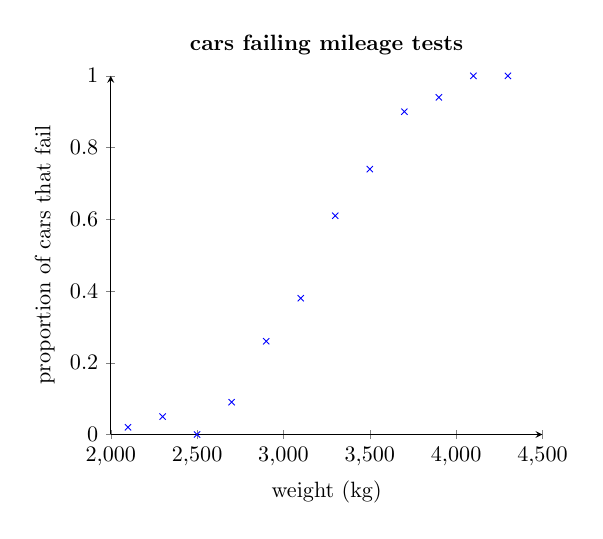
\begin{tikzpicture}[scale=0.8]
			\begin{axis}[
			xmin=2000, xmax=4500, xlabel=weight (kg),
			ymin=0, ymax=1, ylabel=proportion of cars that fail,
			title=\textbf{cars failing mileage tests},
			axis x line=bottom,
			axis y line=left,
			]
			\addplot[blue, only marks, mark=x] coordinates {
				(2100.00,0.02)
				(2300.00,0.05)
				(2500.00,0.00)
				(2700.00,0.09)
				(2900.00,0.26)
				(3100.00,0.38)
				(3300.00,0.61)
				(3500.00,0.74)
				(3700.00,0.90)
				(3900.00,0.94)
				(4100.00,1.00)
				(4300.00,1.00)
			};
			\end{axis}
		\end{tikzpicture}
		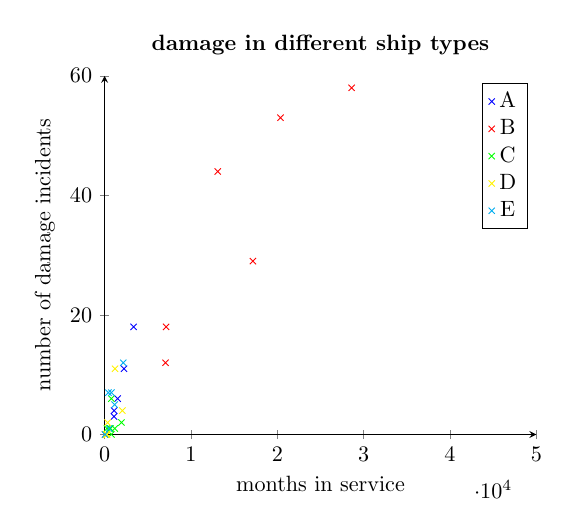
\begin{tikzpicture}[scale=0.8]
		\begin{axis}[
		xmin=0, xmax=50000, xlabel=months in service,
		ymin=0, ymax=60, ylabel=number of damage incidents,
		title=\textbf{damage in different ship types},
		axis x line=bottom,
		axis y line=left,
		]
		\addplot[blue, only marks, mark=x] coordinates {
			(127.00,0.00)
			(63.00,0.00)
			(1095.00,3.00)
			(1095.00,4.00)
			(1512.00,6.00)
			(3353.00,18.00)
			(2244.00,11.00)
		};
		\addlegendentry {A};
		\addplot[red, only marks, mark=x] coordinates {
			(44882.00,39.00)
			(17176.00,29.00)
			(28609.00,58.00)
			(20370.00,53.00)
			(7064.00,12.00)
			(13099.00,44.00)
			(7117.00,18.00)
		};
		\addlegendentry {B};
		\addplot[green, only marks, mark=x] coordinates {
			(1179.00,1.00)
			(552.00,1.00)
			(781.00,0.00)
			(676.00,1.00)
			(783.00,6.00)
			(1948.00,2.00)
			(274.00,1.00)
		};
		\addlegendentry {C};
		\addplot[yellow, only marks, mark=x] coordinates {
			(251.00,0.00)
			(105.00,0.00)
			(288.00,0.00)
			(192.00,0.00)
			(349.00,2.00)
			(1208.00,11.00)
			(2051.00,4.00)
		};
		\addlegendentry {D};
		\addplot[cyan, only marks, mark=x] coordinates {
			(45.00,0.00)
			(789.00,7.00)
			(437.00,7.00)
			(1157.00,5.00)
			(2161.00,12.00)
			(542.00,1.00)
		};
		\addlegendentry {E};
		\end{axis}
		\end{tikzpicture}
	\end{center}
	
	The normal distribution for the errors $\epsilon$ is not appropriate here.
\end{example}

There is a more general class of models than linear models, called \begriff{Generalised Linear Models} (GLMs). They can be written as
\begin{align}
	\mathbb{E}(Y_i) &\equiv \mu_i =\gamma(X_i\beta) \notag \\
	Y_i &\overset{\text{independent}}{\sim} \text{ Exponential family distribution} \notag
\end{align}
where $\gamma$ is any smooth monotonic function. The Exponential family of distributions includes distributions such as Poisson, Gaussian, binomial and gamma.

GLMs are written in terms of the \begriff{link function}, $g$, which is the inverse of $\gamma$:
\begin{align}
	g(\mu_i) &= X_i\beta \notag \\
	Y_i &\overset{\text{independent}}{\sim} \text{ Exponential family distribution} \notag
\end{align}

\begin{example}
	\begin{align}
		Y_i &\sim \text{Binomial} \notag \\
		g(\mu) &= \ln\left(\frac{\mu}{1-\mu}\right)\notag
	\end{align}
	logit link function.
\end{example}

\begin{example}
	Linear models are a special case of GLMs.
\end{example}

The link functions in the following table are only examples. Other link functions can be used with distributions.
\begin{center}
	\begin{tabular}{c|c|c|c|c}
		\textbf{distribution} & \textbf{support} & \text{use} & \textbf{link name} & \textbf{link function} \\
		\hline
		normal & $(-\infty,\infty)$ & linear response & identity & $\mu$ \\
		exponential & $(0,\infty)$ & exponential response & inverse & $\mu^{-1}$ \\
		gamma & $(0,\infty)$ & gamma response & log & $\ln(\mu)$ \\
		Poisson & $\natur_0$ & count data & log & $\ln(\mu)$ \\
		binomial & & proportions of yes/no occurrences & logit & $\ln\left(\frac{\mu}{1-\mu}\right)$
	\end{tabular}
\end{center}

\begin{example}
	AIDS cases per year in Belgium at the start of the epidemic
	\begin{center}
		\begin{tikzpicture}
			\begin{axis}[
			xmin=0, xmax=13, xlabel=year since 1980,
			ymin=0, ymax=250, ylabel=new AIDS cases,
			axis x line=bottom,
			axis y line=left,
			]
			\addplot[blue, only marks, mark=x] coordinates {
				(1,10)
				(2,15)
				(3,30)
				(4,55)
				(5,65)
				(6,70)
				(7,130)
				(8,150)
				(9,170)
				(10,210)
				(11,250)
				(12,245)
				(13,240)
			};
			\end{axis}
		\end{tikzpicture}
	\end{center}
	Early in an epidemic, an exponential increase in cases can occur
	\begin{align}
		\mathbb{E}(Y_i) &\equiv \mu_i = \delta\exp(\alpha t_i) \notag \\
		Y_i &\sim Poisson(\mu_i) \notag
	\end{align}
	Taking the logarithm of both sides and letting $\beta_0\equiv\log(\delta)$ and $\beta_1\equiv\alpha$
	\begin{align}
		\log(\mu_i) &= \beta_0 + \beta_1 t_i \notag \\
		Y_i &\sim Poisson(\mu_i) \notag
	\end{align}
	which is a GLM with a log link.
\end{example}

\subsection{Model fitting in GLMs}

To fit GLMs to data, we use the principle of Maximum Likelihood Estimation (MLE). Given parameters $\beta$, we can write down $f(Y\mid \beta)$, the probability or probability density function of the response $Y$. For observed data, $Y_i^{\text{obs}}$, the likelihood function is
\begin{align}
	L(\beta) = \prod_i f(Y_i^{\text{obs}}\mid \beta)\notag
\end{align}
For GLMs, there is no closed form solution for the values of $\beta$ that maximise this function. Instead, MLE is performed numerically, using a technique called \begriff{iteratively re-weighted least squares} (IRLS). In principle, other optimisation algorithms could also be used for MLE.

\begin{example}[logistic regression]
	The proportion of cars of various weights that fail a mileage test.
	
	\begin{center}
		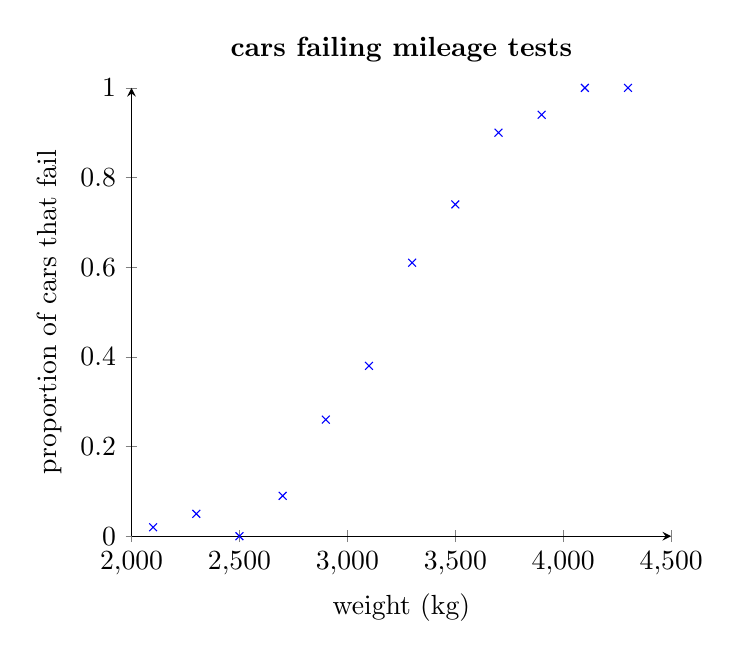
\begin{tikzpicture}
		\begin{axis}[
		xmin=2000, xmax=4500, xlabel=weight (kg),
		ymin=0, ymax=1, ylabel=proportion of cars that fail,
		title=\textbf{cars failing mileage tests},
		axis x line=bottom,
		axis y line=left,
		]
		\addplot[blue, only marks, mark=x] coordinates {
			(2100.00,0.02)
			(2300.00,0.05)
			(2500.00,0.00)
			(2700.00,0.09)
			(2900.00,0.26)
			(3100.00,0.38)
			(3300.00,0.61)
			(3500.00,0.74)
			(3700.00,0.90)
			(3900.00,0.94)
			(4100.00,1.00)
			(4300.00,1.00)
		};
		\end{axis}
		\end{tikzpicture}
	\end{center}
	
	Data are bounded, so LM is not appropriate and we fit a GLM with
	\begin{align}
		Y_i &\sim Binomial(\mu_i) \notag \\
		g(\mu_i) &= X_i\beta = \beta_0 + \beta_1\cdot weight_i \notag
	\end{align}
	Here $g(\mu_i) = \ln\left(\frac{\mu_i}{1-\mu_i}\right)$, so $\mu_i=\frac{1}{1+\exp(-X_i\beta)}$, the logistic function.
\end{example}

\subsection{GLM assumptions and checking}

Important GLM assumptions:
\begin{itemize}
	\item Independence
	\item Distributional assumptions
	\item Weak exogeneity
	\item Linear relationship between transformed response and predictors (link function)
\end{itemize}
Residual plots are still useful to check if model assumptions hold.

As we use different distributions, we cannot simply use raw residuals, as for linear models. Two common types of residuals that attempt to mimic behaviour of residuals for LMs:
\begin{itemize}
	\item \person{Pearson} Residuals
	\item Deviance Residuals
\end{itemize}

Residual plots using deviance residuals.

\begin{center}
	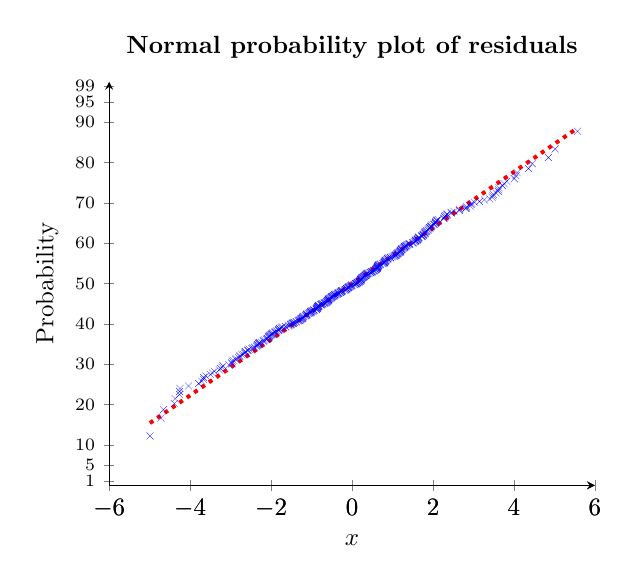
\begin{tikzpicture}[scale=0.9]
	\begin{axis}[
	xmin=-6, xmax=6, xlabel=$x$,
	ymin=-4, ymax=4, ylabel=$y$,
	samples=400,
	axis x line=bottom,
	axis y line=none,
	domain=-6:-6,
	title=\textbf{Normal probability plot of residuals}
	]
	\addplot[mark=x,blue, only marks, ultra thin] coordinates {
		(-4.99,-3.02)
		(-4.72,-2.67)
		(-4.66,-2.50)
		(-4.39,-2.38)
		(-4.37,-2.28)
		(-4.26,-2.20)
		(-4.26,-2.14)
		(-4.25,-2.08)
		(-4.04,-2.03)
		(-3.79,-1.98)
		(-3.71,-1.94)
		(-3.67,-1.90)
		(-3.67,-1.86)
		(-3.61,-1.83)
		(-3.50,-1.80)
		(-3.45,-1.77)
		(-3.40,-1.74)
		(-3.28,-1.71)
		(-3.25,-1.68)
		(-3.21,-1.66)
		(-3.19,-1.63)
		(-3.04,-1.61)
		(-2.97,-1.59)
		(-2.97,-1.57)
		(-2.96,-1.54)
		(-2.94,-1.52)
		(-2.88,-1.50)
		(-2.86,-1.49)
		(-2.80,-1.47)
		(-2.77,-1.45)
		(-2.77,-1.43)
		(-2.72,-1.41)
		(-2.69,-1.40)
		(-2.65,-1.38)
		(-2.64,-1.36)
		(-2.63,-1.35)
		(-2.58,-1.33)
		(-2.57,-1.32)
		(-2.54,-1.30)
		(-2.47,-1.29)
		(-2.45,-1.27)
		(-2.41,-1.26)
		(-2.35,-1.25)
		(-2.35,-1.23)
		(-2.34,-1.22)
		(-2.33,-1.21)
		(-2.31,-1.19)
		(-2.30,-1.18)
		(-2.28,-1.17)
		(-2.24,-1.16)
		(-2.19,-1.14)
		(-2.19,-1.13)
		(-2.16,-1.12)
		(-2.11,-1.11)
		(-2.10,-1.10)
		(-2.09,-1.09)
		(-2.07,-1.07)
		(-2.06,-1.06)
		(-2.05,-1.05)
		(-2.04,-1.04)
		(-2.03,-1.03)
		(-2.01,-1.02)
		(-1.99,-1.01)
		(-1.98,-1.00)
		(-1.97,-0.99)
		(-1.96,-0.98)
		(-1.91,-0.97)
		(-1.90,-0.96)
		(-1.88,-0.95)
		(-1.86,-0.94)
		(-1.82,-0.93)
		(-1.81,-0.92)
		(-1.81,-0.91)
		(-1.79,-0.90)
		(-1.79,-0.89)
		(-1.75,-0.88)
		(-1.73,-0.87)
		(-1.72,-0.86)
		(-1.64,-0.86)
		(-1.64,-0.85)
		(-1.57,-0.84)
		(-1.56,-0.83)
		(-1.52,-0.82)
		(-1.52,-0.81)
		(-1.50,-0.80)
		(-1.47,-0.79)
		(-1.45,-0.78)
		(-1.45,-0.78)
		(-1.42,-0.77)
		(-1.38,-0.76)
		(-1.38,-0.75)
		(-1.33,-0.74)
		(-1.31,-0.73)
		(-1.31,-0.73)
		(-1.28,-0.72)
		(-1.27,-0.71)
		(-1.26,-0.70)
		(-1.25,-0.69)
		(-1.23,-0.69)
		(-1.22,-0.68)
		(-1.22,-0.67)
		(-1.21,-0.66)
		(-1.21,-0.65)
		(-1.19,-0.65)
		(-1.15,-0.64)
		(-1.14,-0.63)
		(-1.13,-0.62)
		(-1.12,-0.62)
		(-1.12,-0.61)
		(-1.11,-0.60)
		(-1.08,-0.59)
		(-1.06,-0.59)
		(-1.04,-0.58)
		(-1.02,-0.57)
		(-1.02,-0.56)
		(-1.01,-0.56)
		(-1.01,-0.55)
		(-0.99,-0.54)
		(-0.96,-0.54)
		(-0.94,-0.53)
		(-0.94,-0.52)
		(-0.89,-0.51)
		(-0.88,-0.51)
		(-0.88,-0.50)
		(-0.87,-0.49)
		(-0.86,-0.49)
		(-0.86,-0.48)
		(-0.85,-0.47)
		(-0.85,-0.46)
		(-0.84,-0.46)
		(-0.83,-0.45)
		(-0.83,-0.44)
		(-0.82,-0.44)
		(-0.82,-0.43)
		(-0.77,-0.42)
		(-0.76,-0.42)
		(-0.75,-0.41)
		(-0.74,-0.40)
		(-0.72,-0.40)
		(-0.69,-0.39)
		(-0.67,-0.38)
		(-0.65,-0.38)
		(-0.63,-0.37)
		(-0.62,-0.36)
		(-0.62,-0.36)
		(-0.62,-0.35)
		(-0.60,-0.34)
		(-0.60,-0.34)
		(-0.59,-0.33)
		(-0.58,-0.32)
		(-0.58,-0.32)
		(-0.58,-0.31)
		(-0.57,-0.30)
		(-0.55,-0.30)
		(-0.54,-0.29)
		(-0.52,-0.28)
		(-0.51,-0.28)
		(-0.51,-0.27)
		(-0.50,-0.26)
		(-0.48,-0.26)
		(-0.47,-0.25)
		(-0.45,-0.24)
		(-0.44,-0.24)
		(-0.43,-0.23)
		(-0.43,-0.22)
		(-0.42,-0.22)
		(-0.40,-0.21)
		(-0.36,-0.21)
		(-0.36,-0.20)
		(-0.35,-0.19)
		(-0.34,-0.19)
		(-0.32,-0.18)
		(-0.29,-0.17)
		(-0.28,-0.17)
		(-0.27,-0.16)
		(-0.26,-0.15)
		(-0.26,-0.15)
		(-0.25,-0.14)
		(-0.24,-0.14)
		(-0.19,-0.13)
		(-0.17,-0.12)
		(-0.16,-0.12)
		(-0.14,-0.11)
		(-0.13,-0.10)
		(-0.13,-0.10)
		(-0.11,-0.09)
		(-0.10,-0.08)
		(-0.09,-0.08)
		(-0.09,-0.07)
		(-0.08,-0.07)
		(-0.07,-0.06)
		(-0.04,-0.05)
		(-0.03,-0.05)
		(-0.02,-0.04)
		(-0.01,-0.03)
		(-0.00,-0.03)
		(0.05,-0.02)
		(0.07,-0.02)
		(0.09,-0.01)
		(0.09,-0.00)
		(0.11,0.00)
		(0.13,0.01)
		(0.13,0.02)
		(0.14,0.02)
		(0.16,0.03)
		(0.17,0.03)
		(0.18,0.04)
		(0.19,0.05)
		(0.20,0.05)
		(0.20,0.06)
		(0.21,0.07)
		(0.22,0.07)
		(0.22,0.08)
		(0.22,0.08)
		(0.23,0.09)
		(0.23,0.10)
		(0.23,0.10)
		(0.24,0.11)
		(0.25,0.12)
		(0.27,0.12)
		(0.28,0.13)
		(0.29,0.14)
		(0.30,0.14)
		(0.31,0.15)
		(0.31,0.15)
		(0.33,0.16)
		(0.33,0.17)
		(0.35,0.17)
		(0.35,0.18)
		(0.36,0.19)
		(0.37,0.19)
		(0.38,0.20)
		(0.40,0.21)
		(0.43,0.21)
		(0.46,0.22)
		(0.47,0.22)
		(0.49,0.23)
		(0.49,0.24)
		(0.50,0.24)
		(0.53,0.25)
		(0.54,0.26)
		(0.55,0.26)
		(0.58,0.27)
		(0.58,0.28)
		(0.58,0.28)
		(0.60,0.29)
		(0.60,0.30)
		(0.62,0.30)
		(0.62,0.31)
		(0.62,0.32)
		(0.63,0.32)
		(0.63,0.33)
		(0.63,0.34)
		(0.64,0.34)
		(0.64,0.35)
		(0.65,0.36)
		(0.66,0.36)
		(0.66,0.37)
		(0.67,0.38)
		(0.70,0.38)
		(0.70,0.39)
		(0.75,0.40)
		(0.78,0.40)
		(0.79,0.41)
		(0.80,0.42)
		(0.80,0.42)
		(0.80,0.43)
		(0.80,0.44)
		(0.82,0.44)
		(0.82,0.45)
		(0.83,0.46)
		(0.83,0.46)
		(0.85,0.47)
		(0.86,0.48)
		(0.88,0.49)
		(0.88,0.49)
		(0.88,0.50)
		(0.90,0.51)
		(0.95,0.51)
		(0.95,0.52)
		(0.99,0.53)
		(1.01,0.54)
		(1.04,0.54)
		(1.05,0.55)
		(1.07,0.56)
		(1.08,0.56)
		(1.09,0.57)
		(1.10,0.58)
		(1.11,0.59)
		(1.13,0.59)
		(1.13,0.60)
		(1.14,0.61)
		(1.16,0.62)
		(1.18,0.62)
		(1.19,0.63)
		(1.19,0.64)
		(1.20,0.65)
		(1.20,0.65)
		(1.20,0.66)
		(1.22,0.67)
		(1.22,0.68)
		(1.23,0.69)
		(1.24,0.69)
		(1.26,0.70)
		(1.28,0.71)
		(1.29,0.72)
		(1.30,0.73)
		(1.30,0.73)
		(1.32,0.74)
		(1.33,0.75)
		(1.35,0.76)
		(1.37,0.77)
		(1.40,0.78)
		(1.41,0.78)
		(1.43,0.79)
		(1.50,0.80)
		(1.50,0.81)
		(1.52,0.82)
		(1.55,0.83)
		(1.57,0.84)
		(1.57,0.85)
		(1.57,0.86)
		(1.60,0.86)
		(1.62,0.87)
		(1.62,0.88)
		(1.63,0.89)
		(1.64,0.90)
		(1.65,0.91)
		(1.65,0.92)
		(1.72,0.93)
		(1.73,0.94)
		(1.73,0.95)
		(1.76,0.96)
		(1.76,0.97)
		(1.77,0.98)
		(1.80,0.99)
		(1.80,1.00)
		(1.80,1.01)
		(1.80,1.02)
		(1.82,1.03)
		(1.84,1.04)
		(1.85,1.05)
		(1.88,1.06)
		(1.88,1.07)
		(1.90,1.09)
		(1.92,1.10)
		(1.92,1.11)
		(1.94,1.12)
		(1.95,1.13)
		(1.95,1.14)
		(1.97,1.16)
		(2.02,1.17)
		(2.03,1.18)
		(2.06,1.19)
		(2.06,1.21)
		(2.07,1.22)
		(2.07,1.23)
		(2.09,1.25)
		(2.10,1.26)
		(2.13,1.27)
		(2.26,1.29)
		(2.28,1.30)
		(2.29,1.32)
		(2.29,1.33)
		(2.31,1.35)
		(2.34,1.36)
		(2.35,1.38)
		(2.45,1.40)
		(2.45,1.41)
		(2.52,1.43)
		(2.65,1.45)
		(2.66,1.47)
		(2.81,1.49)
		(2.82,1.50)
		(2.83,1.52)
		(2.92,1.54)
		(2.94,1.57)
		(2.96,1.59)
		(3.03,1.61)
		(3.15,1.63)
		(3.27,1.66)
		(3.40,1.68)
		(3.46,1.71)
		(3.48,1.74)
		(3.49,1.77)
		(3.56,1.80)
		(3.61,1.83)
		(3.62,1.86)
		(3.63,1.90)
		(3.72,1.94)
		(3.76,1.98)
		(3.82,2.03)
		(4.01,2.08)
		(4.05,2.14)
		(4.08,2.20)
		(4.36,2.28)
		(4.45,2.38)
		(4.85,2.50)
		(5.02,2.67)
		(5.57,3.02)
	};
	\addplot[dotted,red,ultra thick] coordinates {
		(-4.9938,-2.7658)
		(5.5747,3.0865)
	};
	\end{axis}
	\begin{axis}[
	xmin=-6,
	xmax=6,
	ymin=0,
	ymax=100,
	ylabel=Probability,
	axis y line=left,
	axis x line=bottom,
	yticklabel style={font=\scriptsize},
	ytick={1,5,10,20,30,40,50,60,70,80,90,95,99},
	]
	\end{axis}
	\end{tikzpicture}
	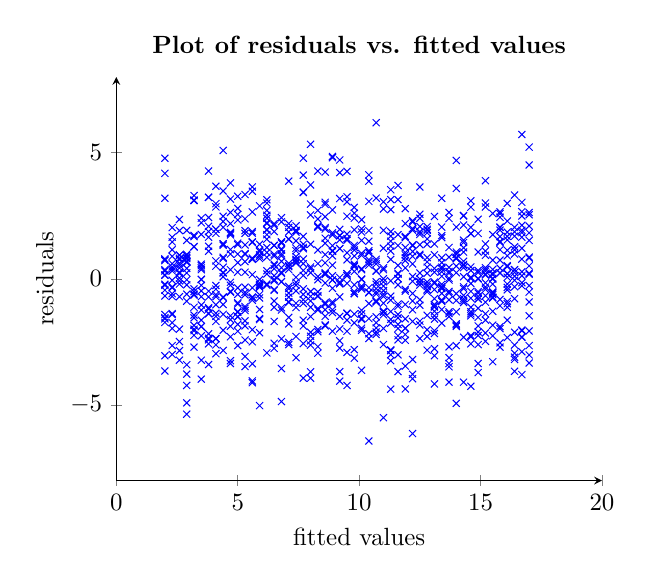
\begin{tikzpicture}[scale=0.9]
	\begin{axis}[
	xmin=0, xmax=20, xlabel=fitted values,
	ymin=-8, ymax=8, ylabel=residuals,
	samples=400,
	axis x line=bottom,
	axis y line=left,
	domain=0:20,
	title=\textbf{Plot of residuals vs. fitted values}
	]
	\addplot[mark=x,blue, only marks] coordinates {
		(2.00,-0.26)
		(2.00,-1.54)
		(2.00,4.78)
		(2.00,0.15)
		(2.00,0.75)
		(2.00,0.79)
		(2.00,-0.22)
		(2.00,-3.66)
		(2.00,4.18)
		(2.00,0.72)
		(2.00,-1.59)
		(2.00,-0.45)
		(2.00,3.19)
		(2.00,0.31)
		(2.00,0.36)
		(2.00,-0.68)
		(2.00,-3.05)
		(2.00,-1.42)
		(2.00,-1.73)
		(2.00,0.14)
		(2.30,0.31)
		(2.30,-0.36)
		(2.30,1.46)
		(2.30,-0.70)
		(2.30,0.47)
		(2.30,-1.74)
		(2.30,-1.97)
		(2.30,-0.59)
		(2.30,1.65)
		(2.30,0.39)
		(2.30,0.60)
		(2.30,-1.42)
		(2.30,-1.38)
		(2.30,1.15)
		(2.30,0.89)
		(2.30,-2.65)
		(2.30,-3.00)
		(2.30,2.03)
		(2.30,-0.06)
		(2.30,-0.32)
		(2.60,0.76)
		(2.60,-0.21)
		(2.60,0.43)
		(2.60,0.94)
		(2.60,-3.23)
		(2.60,0.03)
		(2.60,-0.08)
		(2.60,0.81)
		(2.60,0.61)
		(2.60,-2.49)
		(2.60,0.26)
		(2.60,-2.00)
		(2.60,-0.71)
		(2.60,0.21)
		(2.60,1.91)
		(2.60,0.93)
		(2.60,0.53)
		(2.60,-2.85)
		(2.60,0.22)
		(2.60,2.35)
		(2.90,-4.23)
		(2.90,0.92)
		(2.90,-4.92)
		(2.90,-0.61)
		(2.90,0.80)
		(2.90,-3.41)
		(2.90,1.52)
		(2.90,0.41)
		(2.90,1.92)
		(2.90,0.97)
		(2.90,-0.89)
		(2.90,0.65)
		(2.90,-0.04)
		(2.90,-3.78)
		(2.90,0.68)
		(2.90,0.68)
		(2.90,0.85)
		(2.90,0.23)
		(2.90,-0.24)
		(2.90,-5.37)
		(3.20,3.10)
		(3.20,-1.85)
		(3.20,-1.44)
		(3.20,1.67)
		(3.20,-1.13)
		(3.20,-2.00)
		(3.20,1.28)
		(3.20,-0.51)
		(3.20,-2.24)
		(3.20,3.30)
		(3.20,-0.61)
		(3.20,-1.55)
		(3.20,-2.71)
		(3.20,-0.65)
		(3.20,3.11)
		(3.20,1.26)
		(3.20,-2.06)
		(3.20,-0.40)
		(3.20,1.72)
		(3.20,3.12)
		(3.50,-0.26)
		(3.50,-1.64)
		(3.50,0.58)
		(3.50,-2.26)
		(3.50,1.76)
		(3.50,-1.89)
		(3.50,-1.24)
		(3.50,-3.98)
		(3.50,-1.90)
		(3.50,0.52)
		(3.50,2.40)
		(3.50,2.22)
		(3.50,-3.23)
		(3.50,-0.71)
		(3.50,-0.02)
		(3.50,-0.03)
		(3.50,0.43)
		(3.50,0.36)
		(3.50,-1.04)
		(3.50,-0.48)
		(3.80,-1.39)
		(3.80,-1.37)
		(3.80,1.87)
		(3.80,-2.42)
		(3.80,-0.72)
		(3.80,-2.36)
		(3.80,1.29)
		(3.80,-2.18)
		(3.80,-3.40)
		(3.80,-2.58)
		(3.80,1.09)
		(3.80,4.27)
		(3.80,-1.15)
		(3.80,1.65)
		(3.80,3.23)
		(3.80,2.43)
		(3.80,3.23)
		(3.80,-1.20)
		(3.80,2.08)
		(3.80,-0.49)
		(4.10,-2.97)
		(4.10,-0.71)
		(4.10,0.71)
		(4.10,3.67)
		(4.10,1.80)
		(4.10,0.50)
		(4.10,1.97)
		(4.10,-1.03)
		(4.10,-2.62)
		(4.10,-1.37)
		(4.10,-2.37)
		(4.10,1.96)
		(4.10,-0.27)
		(4.10,-2.38)
		(4.10,-0.41)
		(4.10,-1.69)
		(4.10,-0.63)
		(4.10,2.85)
		(4.10,2.98)
		(4.10,-1.49)
		(4.40,-0.75)
		(4.40,0.85)
		(4.40,0.23)
		(4.40,-1.02)
		(4.40,2.04)
		(4.40,-2.84)
		(4.40,5.09)
		(4.40,-0.72)
		(4.40,0.80)
		(4.40,-1.41)
		(4.40,-2.04)
		(4.40,2.27)
		(4.40,0.08)
		(4.40,0.46)
		(4.40,0.25)
		(4.40,1.39)
		(4.40,3.48)
		(4.40,1.33)
		(4.40,1.38)
		(4.40,2.48)
		(4.70,1.80)
		(4.70,-2.30)
		(4.70,-0.53)
		(4.70,-3.25)
		(4.70,1.16)
		(4.70,3.80)
		(4.70,3.16)
		(4.70,1.84)
		(4.70,-1.88)
		(4.70,-1.47)
		(4.70,0.36)
		(4.70,-0.26)
		(4.70,1.74)
		(4.70,2.63)
		(4.70,-0.50)
		(4.70,-0.14)
		(4.70,2.19)
		(4.70,0.98)
		(4.70,-3.36)
		(4.70,-1.62)
		(5.00,-1.50)
		(5.00,-2.65)
		(5.00,-0.36)
		(5.00,0.26)
		(5.00,2.79)
		(5.00,1.41)
		(5.00,2.33)
		(5.00,-1.51)
		(5.00,0.64)
		(5.00,3.27)
		(5.00,-1.30)
		(5.00,1.35)
		(5.00,2.55)
		(5.00,-2.08)
		(5.00,0.98)
		(5.00,-1.81)
		(5.00,-0.95)
		(5.00,-1.33)
		(5.00,-1.00)
		(5.00,-0.62)
		(5.30,-1.67)
		(5.30,-1.26)
		(5.30,1.00)
		(5.30,3.34)
		(5.30,-3.08)
		(5.30,-0.54)
		(5.30,0.68)
		(5.30,0.97)
		(5.30,1.91)
		(5.30,0.26)
		(5.30,-3.48)
		(5.30,1.34)
		(5.30,1.80)
		(5.30,-1.10)
		(5.30,-0.64)
		(5.30,-1.17)
		(5.30,-0.33)
		(5.30,-1.87)
		(5.30,2.38)
		(5.30,-2.43)
		(5.60,-0.76)
		(5.60,2.65)
		(5.60,0.77)
		(5.60,-0.72)
		(5.60,-0.85)
		(5.60,0.77)
		(5.60,1.81)
		(5.60,1.44)
		(5.60,3.47)
		(5.60,-2.02)
		(5.60,-0.36)
		(5.60,-4.05)
		(5.60,0.82)
		(5.60,1.47)
		(5.60,0.16)
		(5.60,-3.37)
		(5.60,-4.12)
		(5.60,3.64)
		(5.60,-2.50)
		(5.60,1.87)
		(5.90,-0.34)
		(5.90,-0.16)
		(5.90,-1.22)
		(5.90,1.14)
		(5.90,-0.31)
		(5.90,-2.14)
		(5.90,-0.63)
		(5.90,-0.03)
		(5.90,-0.26)
		(5.90,0.89)
		(5.90,0.80)
		(5.90,-5.03)
		(5.90,-1.58)
		(5.90,-0.23)
		(5.90,0.95)
		(5.90,1.37)
		(5.90,1.08)
		(5.90,-0.76)
		(5.90,2.89)
		(5.90,-1.62)
		(6.20,-2.94)
		(6.20,0.85)
		(6.20,1.93)
		(6.20,1.94)
		(6.20,1.04)
		(6.20,1.75)
		(6.20,0.32)
		(6.20,3.13)
		(6.20,2.71)
		(6.20,0.19)
		(6.20,1.57)
		(6.20,2.22)
		(6.20,3.00)
		(6.20,-0.26)
		(6.20,2.52)
		(6.20,2.19)
		(6.20,1.95)
		(6.20,2.40)
		(6.20,-0.21)
		(6.20,1.24)
		(6.50,2.18)
		(6.50,-0.88)
		(6.50,-2.56)
		(6.50,1.32)
		(6.50,0.40)
		(6.50,0.90)
		(6.50,-0.03)
		(6.50,-1.69)
		(6.50,0.97)
		(6.50,1.87)
		(6.50,0.58)
		(6.50,-0.43)
		(6.50,-0.08)
		(6.50,-0.46)
		(6.50,-2.76)
		(6.50,0.53)
		(6.50,2.12)
		(6.50,0.12)
		(6.50,-1.13)
		(6.50,1.33)
		(6.80,2.42)
		(6.80,0.91)
		(6.80,0.99)
		(6.80,0.44)
		(6.80,-1.15)
		(6.80,0.26)
		(6.80,2.26)
		(6.80,-0.11)
		(6.80,1.41)
		(6.80,-0.12)
		(6.80,1.18)
		(6.80,-1.24)
		(6.80,-2.38)
		(6.80,-4.87)
		(6.80,1.46)
		(6.80,0.69)
		(6.80,1.46)
		(6.80,1.14)
		(6.80,-3.56)
		(6.80,0.21)
		(7.10,3.87)
		(7.10,1.86)
		(7.10,-0.30)
		(7.10,-0.94)
		(7.10,-0.73)
		(7.10,0.52)
		(7.10,0.37)
		(7.10,-1.79)
		(7.10,-0.91)
		(7.10,-0.57)
		(7.10,2.19)
		(7.10,2.04)
		(7.10,0.61)
		(7.10,-2.52)
		(7.10,0.48)
		(7.10,1.57)
		(7.10,-0.39)
		(7.10,-2.61)
		(7.10,-1.53)
		(7.10,1.57)
		(7.40,-0.14)
		(7.40,0.77)
		(7.40,0.62)
		(7.40,1.50)
		(7.40,1.91)
		(7.40,0.88)
		(7.40,1.11)
		(7.40,0.73)
		(7.40,-2.29)
		(7.40,1.85)
		(7.40,2.10)
		(7.40,0.66)
		(7.40,-0.48)
		(7.40,-1.14)
		(7.40,-3.13)
		(7.40,0.06)
		(7.40,1.21)
		(7.40,1.92)
		(7.40,-0.25)
		(7.40,-0.97)
		(7.70,3.44)
		(7.70,3.42)
		(7.70,4.78)
		(7.70,-1.87)
		(7.70,-2.57)
		(7.70,0.33)
		(7.70,0.78)
		(7.70,1.37)
		(7.70,-0.98)
		(7.70,-0.40)
		(7.70,-0.62)
		(7.70,-3.94)
		(7.70,-1.64)
		(7.70,0.13)
		(7.70,-0.83)
		(7.70,1.68)
		(7.70,1.19)
		(7.70,0.60)
		(7.70,1.24)
		(7.70,4.11)
		(8.00,-0.50)
		(8.00,5.33)
		(8.00,3.72)
		(8.00,2.53)
		(8.00,-3.94)
		(8.00,-1.13)
		(8.00,-2.63)
		(8.00,0.40)
		(8.00,-2.12)
		(8.00,-0.88)
		(8.00,2.96)
		(8.00,-2.46)
		(8.00,-3.69)
		(8.00,-1.50)
		(8.00,-0.51)
		(8.00,1.37)
		(8.00,0.24)
		(8.00,-0.70)
		(8.00,0.47)
		(8.00,-2.28)
		(8.30,0.60)
		(8.30,2.07)
		(8.30,-0.04)
		(8.30,2.37)
		(8.30,-0.67)
		(8.30,2.04)
		(8.30,-2.69)
		(8.30,0.09)
		(8.30,1.14)
		(8.30,-2.10)
		(8.30,-2.95)
		(8.30,-1.18)
		(8.30,-0.52)
		(8.30,2.71)
		(8.30,-2.01)
		(8.30,2.09)
		(8.30,-0.52)
		(8.30,-1.24)
		(8.30,-0.70)
		(8.30,4.27)
		(8.60,-1.23)
		(8.60,3.03)
		(8.60,0.17)
		(8.60,-1.01)
		(8.60,1.41)
		(8.60,0.24)
		(8.60,-0.17)
		(8.60,0.96)
		(8.60,-0.95)
		(8.60,4.23)
		(8.60,0.20)
		(8.60,1.61)
		(8.60,2.03)
		(8.60,-1.87)
		(8.60,2.95)
		(8.60,1.97)
		(8.60,-1.49)
		(8.60,0.63)
		(8.60,-1.83)
		(8.60,2.46)
		(8.90,-0.05)
		(8.90,1.82)
		(8.90,0.12)
		(8.90,0.54)
		(8.90,-0.99)
		(8.90,-0.92)
		(8.90,-0.38)
		(8.90,4.85)
		(8.90,1.74)
		(8.90,1.12)
		(8.90,1.10)
		(8.90,4.80)
		(8.90,0.91)
		(8.90,1.31)
		(8.90,-1.23)
		(8.90,-0.04)
		(8.90,-2.08)
		(8.90,1.09)
		(8.90,-1.34)
		(8.90,2.73)
		(9.20,1.96)
		(9.20,-0.13)
		(9.20,-0.72)
		(9.20,-2.75)
		(9.20,1.70)
		(9.20,1.72)
		(9.20,-0.20)
		(9.20,4.21)
		(9.20,1.19)
		(9.20,1.20)
		(9.20,0.05)
		(9.20,1.54)
		(9.20,-1.49)
		(9.20,-0.19)
		(9.20,-1.99)
		(9.20,-2.46)
		(9.20,-3.68)
		(9.20,3.18)
		(9.20,-4.06)
		(9.20,4.71)
		(9.50,1.53)
		(9.50,-4.23)
		(9.50,-0.18)
		(9.50,1.77)
		(9.50,-1.38)
		(9.50,1.59)
		(9.50,-2.08)
		(9.50,0.20)
		(9.50,3.05)
		(9.50,0.75)
		(9.50,2.48)
		(9.50,0.13)
		(9.50,-1.36)
		(9.50,1.03)
		(9.50,0.11)
		(9.50,4.26)
		(9.50,-1.64)
		(9.50,0.20)
		(9.50,-2.92)
		(9.50,3.25)
		(9.80,1.32)
		(9.80,2.83)
		(9.80,-0.51)
		(9.80,0.90)
		(9.80,2.60)
		(9.80,-0.59)
		(9.80,1.14)
		(9.80,-2.81)
		(9.80,-0.59)
		(9.80,-0.24)
		(9.80,-1.40)
		(9.80,-3.15)
		(9.80,0.58)
		(9.80,0.48)
		(9.80,1.24)
		(9.80,1.94)
		(9.80,-1.75)
		(9.80,0.52)
		(9.80,0.29)
		(9.80,2.40)
		(10.10,1.85)
		(10.10,-1.57)
		(10.10,-3.63)
		(10.10,-1.62)
		(10.10,1.98)
		(10.10,-0.01)
		(10.10,-0.41)
		(10.10,-1.39)
		(10.10,-1.25)
		(10.10,0.93)
		(10.10,1.52)
		(10.10,1.01)
		(10.10,0.36)
		(10.10,2.34)
		(10.10,-0.36)
		(10.10,-0.03)
		(10.10,-1.96)
		(10.10,0.40)
		(10.10,-0.29)
		(10.10,-2.04)
		(10.40,1.11)
		(10.40,0.54)
		(10.40,4.12)
		(10.40,1.03)
		(10.40,1.04)
		(10.40,-0.35)
		(10.40,-2.18)
		(10.40,-2.37)
		(10.40,0.68)
		(10.40,3.07)
		(10.40,0.76)
		(10.40,1.91)
		(10.40,-0.98)
		(10.40,0.63)
		(10.40,-0.53)
		(10.40,-1.58)
		(10.40,1.49)
		(10.40,-0.56)
		(10.40,-6.43)
		(10.40,3.87)
		(10.70,-0.60)
		(10.70,0.77)
		(10.70,-0.91)
		(10.70,0.31)
		(10.70,-0.52)
		(10.70,-0.12)
		(10.70,-0.87)
		(10.70,-2.21)
		(10.70,-0.92)
		(10.70,0.59)
		(10.70,-0.39)
		(10.70,3.20)
		(10.70,6.19)
		(10.70,-1.51)
		(10.70,-1.74)
		(10.70,-2.11)
		(10.70,-1.95)
		(10.70,-0.22)
		(10.70,0.69)
		(10.70,0.31)
		(11.00,-2.61)
		(11.00,3.05)
		(11.00,1.92)
		(11.00,-1.97)
		(11.00,-0.47)
		(11.00,-0.97)
		(11.00,-0.12)
		(11.00,-1.28)
		(11.00,-1.43)
		(11.00,0.36)
		(11.00,-0.61)
		(11.00,-0.00)
		(11.00,-0.70)
		(11.00,-0.29)
		(11.00,0.43)
		(11.00,-1.31)
		(11.00,2.77)
		(11.00,1.21)
		(11.00,-5.51)
		(11.00,-1.33)
		(11.30,1.29)
		(11.30,1.87)
		(11.30,-2.85)
		(11.30,3.53)
		(11.30,-0.08)
		(11.30,-3.01)
		(11.30,-0.85)
		(11.30,-1.30)
		(11.30,3.14)
		(11.30,-4.38)
		(11.30,-1.61)
		(11.30,0.77)
		(11.30,1.49)
		(11.30,-3.25)
		(11.30,2.74)
		(11.30,-2.82)
		(11.30,-1.76)
		(11.30,-0.69)
		(11.30,1.69)
		(11.30,1.10)
		(11.60,0.01)
		(11.60,1.75)
		(11.60,-1.09)
		(11.60,3.14)
		(11.60,0.18)
		(11.60,-3.68)
		(11.60,-1.81)
		(11.60,-1.97)
		(11.60,-2.26)
		(11.60,1.32)
		(11.60,-2.42)
		(11.60,-0.00)
		(11.60,-0.24)
		(11.60,-1.55)
		(11.60,0.22)
		(11.60,-1.41)
		(11.60,3.70)
		(11.60,-3.02)
		(11.60,0.53)
		(11.60,-1.00)
		(11.90,-0.42)
		(11.90,-3.46)
		(11.90,1.68)
		(11.90,0.43)
		(11.90,2.19)
		(11.90,1.24)
		(11.90,-1.59)
		(11.90,-2.44)
		(11.90,-1.02)
		(11.90,1.04)
		(11.90,-2.21)
		(11.90,-0.49)
		(11.90,-4.37)
		(11.90,-1.97)
		(11.90,0.95)
		(11.90,1.63)
		(11.90,2.78)
		(11.90,0.84)
		(11.90,0.72)
		(11.90,-1.96)
		(12.20,-3.96)
		(12.20,1.99)
		(12.20,1.08)
		(12.20,0.89)
		(12.20,1.31)
		(12.20,-0.88)
		(12.20,2.25)
		(12.20,1.92)
		(12.20,-0.58)
		(12.20,-1.23)
		(12.20,-0.10)
		(12.20,1.34)
		(12.20,2.30)
		(12.20,1.98)
		(12.20,-3.79)
		(12.20,0.59)
		(12.20,-6.14)
		(12.20,-3.20)
		(12.20,-1.69)
		(12.20,0.09)
		(12.50,-0.12)
		(12.50,-0.25)
		(12.50,2.07)
		(12.50,0.23)
		(12.50,1.76)
		(12.50,-0.15)
		(12.50,-1.83)
		(12.50,-2.37)
		(12.50,2.40)
		(12.50,-0.83)
		(12.50,0.97)
		(12.50,-0.01)
		(12.50,-1.05)
		(12.50,0.92)
		(12.50,-1.68)
		(12.50,1.84)
		(12.50,2.56)
		(12.50,3.64)
		(12.50,1.35)
		(12.50,1.87)
		(12.80,1.58)
		(12.80,-2.02)
		(12.80,-0.23)
		(12.80,0.84)
		(12.80,-2.29)
		(12.80,-0.45)
		(12.80,-2.83)
		(12.80,-0.52)
		(12.80,0.46)
		(12.80,0.67)
		(12.80,1.37)
		(12.80,1.96)
		(12.80,-0.43)
		(12.80,1.92)
		(12.80,2.07)
		(12.80,-0.31)
		(12.80,0.22)
		(12.80,1.82)
		(12.80,-0.13)
		(12.80,-1.45)
		(13.10,-1.02)
		(13.10,-1.29)
		(13.10,-2.17)
		(13.10,2.47)
		(13.10,-4.17)
		(13.10,-0.18)
		(13.10,0.26)
		(13.10,0.41)
		(13.10,-0.43)
		(13.10,-3.05)
		(13.10,-1.09)
		(13.10,-2.06)
		(13.10,1.38)
		(13.10,-0.79)
		(13.10,0.95)
		(13.10,-0.13)
		(13.10,-1.12)
		(13.10,-1.47)
		(13.10,-2.77)
		(13.10,-1.60)
		(13.40,-1.22)
		(13.40,-0.22)
		(13.40,0.83)
		(13.40,0.46)
		(13.40,1.71)
		(13.40,0.10)
		(13.40,2.05)
		(13.40,-0.36)
		(13.40,-0.58)
		(13.40,1.63)
		(13.40,0.64)
		(13.40,0.28)
		(13.40,-0.90)
		(13.40,-0.31)
		(13.40,-1.76)
		(13.40,-0.39)
		(13.40,0.39)
		(13.40,3.19)
		(13.40,-0.88)
		(13.40,-0.84)
		(13.70,0.45)
		(13.70,0.29)
		(13.70,0.02)
		(13.70,0.22)
		(13.70,-4.10)
		(13.70,2.63)
		(13.70,1.24)
		(13.70,-0.84)
		(13.70,-1.31)
		(13.70,-1.38)
		(13.70,-3.36)
		(13.70,-0.50)
		(13.70,2.39)
		(13.70,-3.13)
		(13.70,-3.49)
		(13.70,-0.05)
		(13.70,-2.70)
		(13.70,-0.57)
		(13.70,-1.50)
		(13.70,0.86)
		(14.00,-0.86)
		(14.00,0.24)
		(14.00,0.84)
		(14.00,0.81)
		(14.00,0.97)
		(14.00,-0.59)
		(14.00,-4.94)
		(14.00,0.50)
		(14.00,-1.86)
		(14.00,1.06)
		(14.00,-2.65)
		(14.00,2.05)
		(14.00,-1.80)
		(14.00,-1.31)
		(14.00,0.80)
		(14.00,4.69)
		(14.00,-1.89)
		(14.00,3.58)
		(14.00,0.98)
		(14.00,-1.79)
		(14.30,1.53)
		(14.30,0.44)
		(14.30,-0.94)
		(14.30,-0.87)
		(14.30,-4.10)
		(14.30,-0.32)
		(14.30,1.06)
		(14.30,0.53)
		(14.30,-0.66)
		(14.30,2.13)
		(14.30,-0.79)
		(14.30,1.23)
		(14.30,-2.32)
		(14.30,-0.39)
		(14.30,0.57)
		(14.30,1.44)
		(14.30,0.08)
		(14.30,0.69)
		(14.30,2.51)
		(14.30,2.49)
		(14.60,-1.13)
		(14.60,0.47)
		(14.60,3.09)
		(14.60,0.33)
		(14.60,0.06)
		(14.60,2.84)
		(14.60,1.78)
		(14.60,-1.31)
		(14.60,0.01)
		(14.60,-2.25)
		(14.60,-0.50)
		(14.60,1.80)
		(14.60,-2.58)
		(14.60,2.04)
		(14.60,-0.77)
		(14.60,-1.39)
		(14.60,-1.47)
		(14.60,-4.26)
		(14.60,-0.19)
		(14.60,-2.30)
		(14.90,-3.36)
		(14.90,-0.01)
		(14.90,-1.17)
		(14.90,-0.80)
		(14.90,0.25)
		(14.90,0.33)
		(14.90,-0.70)
		(14.90,-0.57)
		(14.90,-0.80)
		(14.90,-0.51)
		(14.90,-1.87)
		(14.90,-2.61)
		(14.90,-2.25)
		(14.90,1.06)
		(14.90,0.01)
		(14.90,1.80)
		(14.90,2.36)
		(14.90,-1.53)
		(14.90,-2.11)
		(14.90,-3.72)
		(15.20,-0.42)
		(15.20,1.38)
		(15.20,3.00)
		(15.20,0.15)
		(15.20,-0.93)
		(15.20,0.44)
		(15.20,-1.64)
		(15.20,0.18)
		(15.20,-0.16)
		(15.20,-2.48)
		(15.20,-0.67)
		(15.20,0.93)
		(15.20,2.85)
		(15.20,1.10)
		(15.20,3.89)
		(15.20,-1.39)
		(15.20,0.37)
		(15.20,-0.33)
		(15.20,0.30)
		(15.20,-2.15)
		(15.50,-0.21)
		(15.50,-0.63)
		(15.50,-0.75)
		(15.50,-0.73)
		(15.50,-0.52)
		(15.50,0.02)
		(15.50,2.59)
		(15.50,-0.76)
		(15.50,-0.01)
		(15.50,-3.29)
		(15.50,0.37)
		(15.50,0.16)
		(15.50,-1.29)
		(15.50,0.74)
		(15.50,-0.57)
		(15.50,-0.54)
		(15.50,-2.26)
		(15.50,1.75)
		(15.50,-1.84)
		(15.50,0.22)
		(15.80,0.24)
		(15.80,1.44)
		(15.80,1.48)
		(15.80,-2.71)
		(15.80,2.58)
		(15.80,1.15)
		(15.80,-1.90)
		(15.80,-1.98)
		(15.80,-0.82)
		(15.80,-1.07)
		(15.80,1.93)
		(15.80,2.04)
		(15.80,0.42)
		(15.80,2.05)
		(15.80,0.22)
		(15.80,2.65)
		(15.80,2.44)
		(15.80,-2.54)
		(15.80,1.67)
		(15.80,0.74)
		(16.10,-0.44)
		(16.10,1.68)
		(16.10,-0.90)
		(16.10,-1.13)
		(16.10,1.13)
		(16.10,-0.21)
		(16.10,0.19)
		(16.10,2.29)
		(16.10,-0.99)
		(16.10,0.48)
		(16.10,1.54)
		(16.10,-2.33)
		(16.10,0.21)
		(16.10,-0.34)
		(16.10,0.91)
		(16.10,0.52)
		(16.10,0.06)
		(16.10,-1.64)
		(16.10,1.85)
		(16.10,2.99)
		(16.40,0.98)
		(16.40,1.69)
		(16.40,0.10)
		(16.40,-0.79)
		(16.40,0.36)
		(16.40,-3.11)
		(16.40,3.32)
		(16.40,1.86)
		(16.40,-3.67)
		(16.40,-2.63)
		(16.40,1.15)
		(16.40,-0.32)
		(16.40,-0.06)
		(16.40,-3.20)
		(16.40,0.25)
		(16.40,0.36)
		(16.40,1.27)
		(16.40,-2.95)
		(16.40,2.04)
		(16.40,-2.12)
		(16.70,0.12)
		(16.70,3.03)
		(16.70,2.66)
		(16.70,0.78)
		(16.70,2.12)
		(16.70,-2.31)
		(16.70,1.65)
		(16.70,1.83)
		(16.70,-2.06)
		(16.70,0.28)
		(16.70,5.72)
		(16.70,1.92)
		(16.70,2.49)
		(16.70,1.21)
		(16.70,-2.32)
		(16.70,-3.80)
		(16.70,-0.16)
		(16.70,-2.03)
		(16.70,-2.89)
		(16.70,-0.28)
		(17.00,0.86)
		(17.00,4.51)
		(17.00,-0.92)
		(17.00,0.18)
		(17.00,5.22)
		(17.00,-2.07)
		(17.00,0.51)
		(17.00,-0.53)
		(17.00,2.63)
		(17.00,0.22)
		(17.00,2.54)
		(17.00,0.82)
		(17.00,1.52)
		(17.00,-3.34)
		(17.00,-1.47)
		(17.00,-2.65)
		(17.00,-3.02)
		(17.00,1.82)
		(17.00,2.09)
		(17.00,-0.27)
	};
	\end{axis}
	\end{tikzpicture}
\end{center}
\begin{center}
	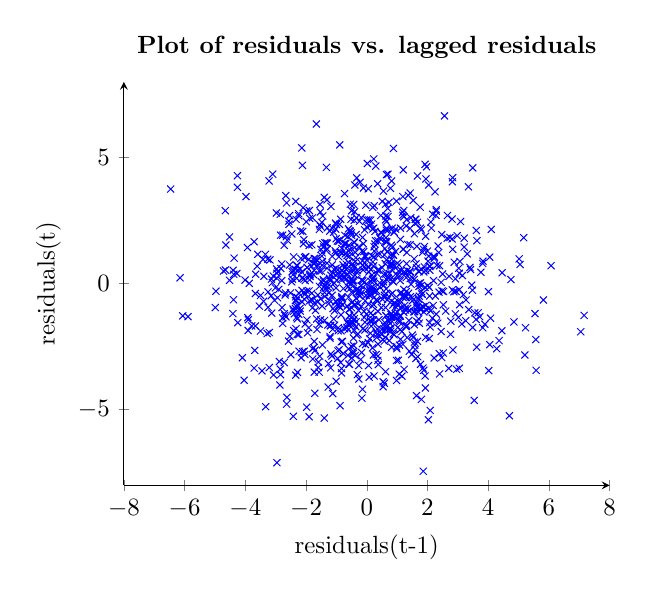
\begin{tikzpicture}[scale=0.9]
	\begin{axis}[
	xmin=-8, xmax=8, xlabel=residuals(t-1),
	ymin=-8, ymax=8, ylabel=residuals(t),
	samples=400,
	axis x line=bottom,
	axis y line=left,
	domain=-8:-8,
	title=\textbf{Plot of residuals vs. lagged residuals}
	]
	\addplot[mark=x,blue, only marks] coordinates {
		(3.67,-1.16)
		(-4.52,1.85)
		(1.72,0.01)
		(0.64,-1.27)
		(-2.62,1.72)
		(-0.87,-0.96)
		(0.69,2.98)
		(7.16,-1.26)
		(5.54,-1.19)
		(-2.70,-1.26)
		(6.07,0.71)
		(1.45,2.61)
		(-0.13,0.73)
		(1.43,1.54)
		(-0.41,2.51)
		(-0.25,-0.26)
		(2.98,1.90)
		(2.82,-0.25)
		(2.83,4.20)
		(1.34,0.52)
		(-2.41,-1.09)
		(1.43,0.20)
		(3.26,-1.47)
		(0.98,-3.05)
		(2.07,0.70)
		(1.45,0.47)
		(-0.61,1.31)
		(0.59,-1.69)
		(-1.57,-1.61)
		(1.78,-0.98)
		(-2.29,-2.01)
		(-2.14,5.38)
		(-1.62,0.74)
		(-5.89,-1.31)
		(2.88,0.85)
		(0.65,2.46)
		(-1.51,1.36)
		(2.74,1.83)
		(-3.42,0.96)
		(-0.20,-3.01)
		(-0.48,-1.52)
		(0.64,2.12)
		(0.63,-0.40)
		(-1.73,0.52)
		(-0.06,1.11)
		(-0.33,-2.04)
		(1.26,0.38)
		(2.19,-0.87)
		(2.22,-2.95)
		(-1.73,0.79)
		(0.15,-1.69)
		(-2.43,-1.01)
		(-2.23,-2.68)
		(-0.01,-1.21)
		(3.07,0.88)
		(-1.54,3.14)
		(0.74,-2.26)
		(-0.45,0.69)
		(2.23,1.05)
		(-2.18,2.09)
		(0.07,2.52)
		(1.11,-2.21)
		(2.20,0.12)
		(3.09,2.46)
		(0.17,1.09)
		(-2.98,2.80)
		(-1.48,2.43)
		(-2.12,4.69)
		(4.70,-5.24)
		(-1.23,-0.66)
		(1.50,-0.68)
		(-0.38,-2.85)
		(1.78,-1.04)
		(-1.53,2.84)
		(-2.80,0.12)
		(-2.84,1.92)
		(0.98,3.27)
		(-0.35,-0.58)
		(-0.39,-0.82)
		(2.84,-2.63)
		(0.58,-0.55)
		(0.40,-1.43)
		(3.18,-0.44)
		(-1.61,-0.45)
		(1.39,-1.46)
		(1.67,-2.29)
		(-0.49,-0.76)
		(0.43,0.03)
		(-2.33,-1.79)
		(-2.30,0.70)
		(0.21,-0.29)
		(1.44,-0.52)
		(5.17,1.82)
		(-1.33,4.61)
		(0.37,1.70)
		(-0.16,1.29)
		(-3.87,0.01)
		(-0.88,0.26)
		(-3.59,1.16)
		(1.68,-1.11)
		(-1.78,-2.99)
		(0.20,0.86)
		(-1.09,-1.40)
		(0.61,0.79)
		(-1.20,-1.66)
		(0.98,-2.51)
		(1.48,-2.81)
		(3.42,0.56)
		(-0.39,3.91)
		(-4.28,0.40)
		(-1.68,0.98)
		(2.71,0.29)
		(-2.14,0.46)
		(1.92,4.73)
		(0.25,-1.56)
		(2.87,-0.32)
		(-3.92,-1.35)
		(-0.40,1.43)
		(-2.42,0.51)
		(5.82,-0.65)
		(1.65,1.48)
		(2.76,-2.01)
		(-2.12,0.24)
		(-0.94,0.40)
		(-0.54,3.15)
		(2.20,1.08)
		(-0.56,0.07)
		(1.40,-2.68)
		(-4.10,-2.94)
		(-0.71,1.18)
		(-1.65,-1.40)
		(-3.15,-0.48)
		(1.02,-1.74)
		(0.56,0.36)
		(0.07,0.46)
		(-2.67,3.49)
		(2.25,3.64)
		(0.70,2.12)
		(-0.60,2.17)
		(0.05,-2.34)
		(-0.52,2.55)
		(-3.50,-1.88)
		(-0.57,-3.20)
		(-1.66,6.33)
		(-1.96,0.64)
		(-2.31,-1.33)
		(-1.07,0.02)
		(-4.01,0.14)
		(1.93,-4.14)
		(1.04,-1.43)
		(-0.04,1.06)
		(-0.07,0.07)
		(-1.60,-3.33)
		(2.04,-0.98)
		(-0.27,-0.30)
		(-1.43,0.16)
		(2.70,-3.36)
		(-0.45,0.51)
		(-1.18,3.06)
		(-0.59,-3.19)
		(-1.70,0.88)
		(-2.24,2.69)
		(5.05,0.76)
		(3.31,1.18)
		(0.62,-0.95)
		(-2.51,-0.37)
		(-1.73,-2.29)
		(-0.35,-0.24)
		(1.58,-1.11)
		(-2.66,-1.32)
		(-4.66,2.89)
		(-2.90,-0.23)
		(0.67,1.26)
		(0.78,0.75)
		(0.90,-2.03)
		(-0.26,-3.78)
		(0.37,-2.87)
		(-0.95,0.55)
		(1.72,-0.60)
		(-2.72,1.52)
		(0.91,-0.76)
		(-1.70,-2.64)
		(-0.67,0.19)
		(1.11,2.20)
		(2.08,0.53)
		(-2.24,-0.37)
		(2.52,-0.84)
		(1.32,2.54)
		(-0.14,1.83)
		(-0.39,-0.86)
		(-0.44,-2.69)
		(-0.61,-1.83)
		(0.05,0.67)
		(0.10,-2.19)
		(1.65,-0.77)
		(3.05,-0.24)
		(0.93,-1.32)
		(-0.42,-1.25)
		(1.25,-0.45)
		(0.37,-1.10)
		(-2.06,-2.68)
		(1.90,1.47)
		(0.61,-1.84)
		(0.27,2.07)
		(1.03,-0.69)
		(0.52,-0.62)
		(-1.88,2.59)
		(-0.32,0.52)
		(-0.29,-0.80)
		(-1.06,-1.65)
		(3.36,-1.03)
		(-1.75,0.80)
		(-0.97,1.69)
		(-1.42,0.10)
		(-2.35,-0.99)
		(-0.38,0.67)
		(-0.55,1.34)
		(3.06,-0.84)
		(-0.50,2.89)
		(-2.13,-0.73)
		(3.21,1.80)
		(2.47,1.94)
		(-0.46,0.11)
		(-3.01,-0.17)
		(-0.89,1.74)
		(-0.31,-3.61)
		(0.55,0.07)
		(-0.52,0.14)
		(0.89,0.73)
		(0.78,-1.77)
		(-2.50,-2.82)
		(-1.90,-5.28)
		(-1.48,1.09)
		(-1.02,2.16)
		(-0.64,-0.89)
		(0.02,4.76)
		(-6.06,-1.28)
		(-0.91,-2.62)
		(2.48,-0.29)
		(-2.13,0.21)
		(1.87,1.36)
		(0.70,0.24)
		(-0.06,-1.53)
		(0.36,-3.05)
		(-3.13,-1.17)
		(-0.17,-2.73)
		(3.21,1.45)
		(0.20,-0.21)
		(0.08,-3.71)
		(-1.47,0.73)
		(-0.06,-1.84)
		(0.46,2.70)
		(0.85,0.10)
		(-0.75,0.46)
		(-0.47,-1.57)
		(4.05,1.05)
		(-4.52,0.13)
		(4.46,0.43)
		(0.68,-0.64)
		(2.00,1.29)
		(-3.33,-4.88)
		(-1.18,0.33)
		(-0.56,2.10)
		(0.85,-0.38)
		(-3.34,1.16)
		(0.94,-1.19)
		(-2.43,0.35)
		(0.13,-1.17)
		(1.30,2.29)
		(0.65,0.94)
		(2.17,2.75)
		(2.01,-0.08)
		(-1.30,-0.12)
		(0.51,0.63)
		(-1.89,2.90)
		(-2.64,-4.78)
		(1.85,-3.35)
		(0.00,2.53)
		(-0.11,3.79)
		(1.82,-0.41)
		(1.19,2.71)
		(0.70,4.34)
		(2.50,0.38)
		(1.86,-0.91)
		(0.48,-0.95)
		(-1.38,-0.51)
		(-1.30,1.60)
		(2.38,-0.34)
		(-3.22,4.07)
		(-0.05,-0.68)
		(-3.90,-1.43)
		(2.04,1.09)
		(1.72,0.47)
		(0.00,0.93)
		(-0.14,-4.19)
		(-4.97,-0.30)
		(1.16,-3.67)
		(-4.38,0.37)
		(-4.64,1.53)
		(0.16,2.36)
		(-1.90,1.51)
		(0.82,0.97)
		(1.35,1.55)
		(1.72,-0.11)
		(-1.38,-0.08)
		(0.90,2.04)
		(0.20,2.17)
		(1.65,-0.94)
		(1.07,-3.59)
		(1.80,-4.59)
		(-0.26,-3.25)
		(-0.29,-2.00)
		(2.02,0.89)
		(-4.25,-1.55)
		(-1.01,-0.17)
		(-2.54,0.74)
		(-0.77,-2.77)
		(1.30,-1.70)
		(1.65,-1.50)
		(-2.03,-1.60)
		(-0.94,-0.88)
		(0.27,1.57)
		(-0.58,-1.01)
		(0.60,1.39)
		(0.80,0.68)
		(-1.86,0.38)
		(-0.35,1.95)
		(-4.26,4.28)
		(2.29,2.93)
		(-1.26,-3.17)
		(-2.41,1.06)
		(-0.51,-2.49)
		(-2.86,-4.02)
		(-0.04,-2.42)
		(-1.12,-4.36)
		(4.36,-2.26)
		(2.28,2.71)
		(-4.99,-0.95)
		(0.88,5.36)
		(-2.80,0.78)
		(-0.51,2.01)
		(0.33,-0.29)
		(1.50,-0.56)
		(-0.55,-1.57)
		(3.15,0.32)
		(-0.96,-2.97)
		(0.66,-1.70)
		(1.33,-2.14)
		(0.17,0.34)
		(1.76,3.03)
		(0.65,4.32)
		(-1.57,-3.51)
		(-3.61,0.69)
		(3.72,-1.31)
		(-1.21,-2.16)
		(0.21,0.21)
		(1.13,-0.94)
		(0.23,0.10)
		(-1.81,1.54)
		(-0.94,-1.87)
		(-0.25,-0.31)
		(2.96,-3.40)
		(-1.72,-0.77)
		(1.57,1.98)
		(0.62,-3.49)
		(-0.47,0.78)
		(-2.11,-2.70)
		(-0.57,0.44)
		(-0.17,-0.90)
		(-2.94,-0.56)
		(0.38,-3.21)
		(-1.64,-1.82)
		(-0.19,-0.39)
		(0.67,0.14)
		(-1.81,-0.38)
		(-0.58,-1.28)
		(0.70,2.66)
		(-3.67,-0.39)
		(2.07,-1.55)
		(4.85,-1.52)
		(1.92,-0.15)
		(-0.63,1.86)
		(0.86,-0.85)
		(-2.07,1.74)
		(3.76,0.45)
		(1.88,-1.13)
		(1.57,-1.63)
		(-1.75,0.35)
		(0.64,-0.21)
		(-1.12,-1.81)
		(-0.62,-1.59)
		(-1.14,1.08)
		(-2.05,1.04)
		(-1.82,-0.62)
		(-0.42,1.65)
		(-3.40,-0.70)
		(1.22,-0.23)
		(-0.24,2.47)
		(1.40,-1.08)
		(0.54,-4.09)
		(0.99,-2.58)
		(-2.97,0.58)
		(-2.04,-0.43)
		(-0.89,5.50)
		(0.22,-2.83)
		(2.26,-0.49)
		(-0.58,0.08)
		(2.52,-2.75)
		(0.95,2.16)
		(2.35,1.49)
		(0.25,3.09)
		(-1.31,1.38)
		(-2.96,-7.10)
		(0.31,-1.93)
		(1.64,0.62)
		(-0.59,-1.63)
		(-1.08,0.57)
		(-0.62,-0.13)
		(-2.19,-1.09)
		(-0.99,0.14)
		(-0.36,1.03)
		(0.09,2.29)
		(-0.13,-1.79)
		(1.22,-1.14)
		(0.22,-1.44)
		(3.63,1.70)
		(0.62,3.15)
		(3.61,2.11)
		(-1.45,2.68)
		(1.05,0.50)
		(-0.52,-1.60)
		(1.20,1.36)
		(1.19,3.45)
		(-4.37,1.01)
		(-2.65,1.86)
		(-2.88,-3.09)
		(0.80,1.14)
		(2.94,-0.31)
		(-0.65,1.11)
		(1.62,2.55)
		(1.09,-1.28)
		(-2.10,3.01)
		(0.79,-1.89)
		(-1.50,0.08)
		(3.03,0.61)
		(-0.07,2.13)
		(3.27,-0.65)
		(-0.85,-1.87)
		(1.18,2.83)
		(-0.13,0.73)
		(-4.04,-3.83)
		(-1.96,0.64)
		(1.23,-3.40)
		(-0.11,1.58)
		(-2.24,2.77)
		(-1.25,-0.37)
		(0.50,-1.82)
		(-1.99,2.45)
		(1.95,-1.02)
		(-1.28,-1.64)
		(3.62,-2.52)
		(-2.16,-2.94)
		(0.40,0.55)
		(-3.04,-0.66)
		(-1.45,1.58)
		(-1.19,-0.11)
		(0.80,-0.42)
		(1.88,-3.44)
		(0.60,-1.55)
		(-0.75,0.21)
		(1.63,-0.86)
		(1.60,2.55)
		(0.24,-3.66)
		(1.14,-0.36)
		(0.83,0.23)
		(-1.97,-1.44)
		(1.52,0.22)
		(-1.31,3.32)
		(-1.21,-2.10)
		(0.35,-0.70)
		(-0.62,-2.84)
		(-0.26,1.46)
		(1.19,-2.41)
		(2.09,-1.72)
		(-0.40,2.85)
		(0.66,1.65)
		(-0.48,-1.51)
		(0.46,2.03)
		(0.88,-1.32)
		(-1.23,0.21)
		(0.55,3.67)
		(1.20,4.51)
		(0.18,-0.89)
		(3.46,-0.06)
		(-1.22,2.08)
		(-1.47,1.22)
		(-3.50,-0.47)
		(1.82,-0.42)
		(1.73,-1.57)
		(-0.16,-4.54)
		(1.80,-0.31)
		(0.37,-2.40)
		(0.58,-0.46)
		(0.23,4.94)
		(0.88,0.07)
		(0.20,3.02)
		(5.57,-2.22)
		(-2.33,2.55)
		(-3.71,-3.35)
		(-2.28,-0.56)
		(-2.19,0.58)
		(-0.87,1.24)
		(-0.34,-0.25)
		(-0.44,-2.16)
		(1.08,-2.44)
		(0.78,-1.44)
		(1.50,-2.04)
		(3.56,-1.16)
		(2.45,-1.90)
		(-2.57,2.48)
		(-4.66,0.54)
		(1.80,0.57)
		(-3.67,-1.68)
		(0.13,0.55)
		(0.07,0.65)
		(4.45,-1.87)
		(-0.14,-2.38)
		(-1.01,-3.87)
		(0.47,1.75)
		(0.49,-2.02)
		(0.14,0.09)
		(-1.22,0.17)
		(-2.45,0.18)
		(0.63,-1.28)
		(-2.69,-0.45)
		(-2.06,-0.61)
		(2.66,2.70)
		(-0.84,-2.31)
		(-0.28,-0.41)
		(1.80,2.13)
		(-0.60,0.84)
		(2.06,-2.18)
		(-0.69,1.59)
		(2.03,-5.40)
		(1.26,-0.99)
		(-0.43,3.14)
		(-1.73,1.00)
		(-2.09,1.58)
		(-0.54,-0.19)
		(-0.88,-0.76)
		(-0.82,1.39)
		(1.97,4.63)
		(-0.60,-0.54)
		(2.29,2.87)
		(-1.06,-1.08)
		(1.95,-0.86)
		(-1.04,1.30)
		(0.35,-1.80)
		(1.94,1.88)
		(-0.83,-3.37)
		(-0.88,-4.84)
		(4.01,-0.32)
		(1.90,0.66)
		(-0.86,2.55)
		(1.30,0.24)
		(-0.72,1.91)
		(1.41,0.48)
		(2.83,1.36)
		(-3.21,-1.94)
		(2.06,-0.15)
		(2.92,-1.20)
		(0.09,-0.47)
		(3.49,4.59)
		(0.31,-2.81)
		(-2.47,0.07)
		(-4.39,-0.64)
		(-0.67,0.76)
		(1.43,3.59)
		(0.63,1.82)
		(0.83,-1.31)
		(-1.15,-2.87)
		(0.29,1.70)
		(-3.28,-1.98)
		(-1.52,-1.43)
		(-1.64,0.93)
		(1.04,-3.04)
		(-0.03,3.11)
		(-2.31,0.21)
		(-0.02,-0.47)
		(-1.38,1.62)
		(-1.33,1.61)
		(1.73,-0.50)
		(0.23,2.20)
		(0.80,0.73)
		(1.77,2.20)
		(0.36,0.53)
		(1.10,-0.38)
		(1.37,3.50)
		(2.34,-1.57)
		(0.95,1.27)
		(2.82,4.04)
		(0.05,-0.83)
		(-0.10,1.27)
		(3.40,0.64)
		(-1.02,-0.70)
		(-0.01,-0.01)
		(1.84,1.24)
		(0.30,4.66)
		(2.81,1.77)
		(2.07,-0.49)
		(0.58,-3.95)
		(-1.56,0.50)
		(1.13,0.52)
		(-2.77,-1.58)
		(0.49,2.02)
		(1.62,0.78)
		(0.43,1.17)
		(1.76,-0.97)
		(4.08,-1.37)
		(1.85,-0.93)
		(0.53,-2.22)
		(1.28,-1.05)
		(0.85,1.45)
		(-2.63,-4.51)
		(-0.83,-3.54)
		(2.45,0.05)
		(-0.09,0.66)
		(1.16,-1.90)
		(-2.01,1.07)
		(0.13,2.52)
		(1.20,1.37)
		(-2.72,-3.13)
		(0.70,-1.46)
		(-0.36,-1.71)
		(-1.88,-0.68)
		(-0.08,-1.34)
		(-3.79,-1.68)
		(-4.26,3.82)
		(-2.35,-0.67)
		(-1.98,-0.30)
		(-2.35,0.57)
		(-3.45,-3.46)
		(0.58,-2.28)
		(-3.19,0.94)
		(0.22,0.70)
		(1.57,-2.32)
		(-0.00,2.25)
		(0.19,-0.13)
		(-0.76,0.28)
		(-2.97,0.22)
		(-0.09,-1.10)
		(1.92,-3.66)
		(3.48,-0.26)
		(-0.86,-3.13)
		(-3.25,-0.33)
		(0.33,0.41)
		(0.75,0.40)
		(-0.45,-2.77)
		(-2.30,0.73)
		(4.05,-2.42)
		(-4.72,0.50)
		(-1.02,1.21)
		(-2.64,3.20)
		(-1.27,-4.10)
		(0.64,1.66)
		(0.28,-0.32)
		(-1.42,-0.15)
		(1.55,-1.12)
		(1.24,0.47)
		(1.29,-0.52)
		(-0.85,-1.24)
		(2.10,-1.08)
		(1.32,1.23)
		(5.02,0.98)
		(2.13,2.20)
		(2.31,0.73)
		(0.11,-0.29)
		(-2.58,-2.28)
		(-0.74,0.63)
		(-1.52,-0.61)
		(-1.13,0.44)
		(1.11,1.75)
		(-1.11,-0.99)
		(-1.79,-0.96)
		(-0.82,-0.52)
		(-0.32,0.43)
		(0.82,4.07)
		(-1.91,-1.75)
		(0.63,2.68)
		(0.16,-0.43)
		(2.65,1.80)
		(-0.43,0.12)
		(-0.27,-1.07)
		(-2.34,-0.52)
		(-2.77,1.92)
		(0.62,2.53)
		(-0.50,1.92)
		(1.01,-1.13)
		(-1.79,-2.58)
		(3.82,0.80)
		(0.24,1.06)
		(2.09,-5.03)
		(-0.45,0.05)
		(-0.33,4.19)
		(1.38,-0.38)
		(1.11,-1.29)
		(-2.24,-2.02)
		(-3.07,-3.62)
		(-2.20,-0.98)
		(-2.83,0.60)
		(0.12,-1.97)
		(-0.82,0.51)
		(-0.74,1.58)
		(-2.72,-1.19)
		(1.56,0.98)
		(0.88,1.13)
		(-0.18,-0.09)
		(2.04,3.91)
		(-1.75,-2.54)
		(0.83,0.55)
		(0.70,-1.85)
		(0.70,-1.44)
		(-1.46,0.88)
		(0.65,2.19)
		(-1.03,0.34)
		(-1.79,2.61)
		(-2.41,-1.86)
		(2.08,0.68)
		(-1.69,-1.06)
		(-0.35,-1.51)
		(-2.42,-5.26)
		(-0.59,1.52)
		(-6.46,3.75)
		(-2.17,1.00)
		(-2.85,2.75)
		(-2.03,0.12)
		(-0.43,-2.46)
		(-0.65,-1.74)
		(3.89,-1.61)
		(-1.14,2.20)
		(-0.50,-0.96)
		(-3.14,0.18)
		(-0.95,-2.67)
		(-2.68,-0.37)
		(0.06,-3.25)
		(1.71,-1.40)
		(0.81,1.52)
		(-1.40,3.42)
		(-3.26,0.97)
		(2.92,0.19)
		(4.10,2.15)
		(0.24,1.46)
		(-1.98,-4.90)
		(2.40,-3.58)
		(-1.19,-1.67)
		(-0.94,-1.75)
		(1.77,-3.20)
		(-2.77,-1.36)
		(-3.91,-1.86)
		(0.84,2.20)
		(0.80,-1.22)
		(0.19,-2.55)
		(0.99,-0.83)
		(2.16,-1.37)
		(1.94,0.52)
		(-1.14,-0.46)
		(1.62,-2.97)
		(0.35,1.16)
		(-1.01,-0.73)
		(-2.39,-1.20)
		(1.29,-1.70)
		(-0.71,1.59)
		(0.09,-0.22)
		(-1.59,-3.11)
		(-3.10,4.34)
		(0.34,-0.68)
		(-0.12,0.54)
		(2.40,0.71)
		(1.60,-2.61)
		(2.11,2.44)
		(-1.50,0.50)
		(-1.87,0.29)
		(-2.54,2.70)
		(1.00,0.32)
		(5.58,-3.44)
		(1.46,-0.03)
		(-1.55,2.33)
		(1.67,2.43)
		(-2.26,0.53)
		(-2.85,-3.39)
		(1.43,2.19)
		(-1.56,-0.11)
		(0.63,0.38)
		(2.81,2.56)
		(0.80,0.81)
		(1.86,-7.44)
		(-3.21,-3.33)
		(1.32,-1.66)
		(4.28,-2.58)
		(1.08,0.31)
		(-3.08,0.30)
		(-0.41,-1.39)
		(-1.00,2.34)
		(0.77,-1.58)
		(0.82,-0.69)
		(0.81,-1.33)
		(-0.73,-1.79)
		(-1.20,0.11)
		(-1.18,-2.79)
		(1.71,-0.62)
		(-3.71,1.66)
		(-0.41,1.63)
		(0.54,-3.89)
		(-1.31,0.81)
		(0.95,-0.92)
		(-0.14,0.90)
		(-1.88,0.34)
		(0.32,-0.63)
		(-0.54,-0.03)
		(-0.82,1.22)
		(-1.42,1.45)
		(0.12,-1.50)
		(-3.69,-2.65)
		(-0.80,-0.84)
		(-1.09,2.04)
		(-1.82,0.69)
		(1.31,0.79)
		(-1.47,-0.89)
		(1.08,-1.53)
		(1.95,4.15)
		(-0.31,-0.21)
		(0.56,-0.07)
		(1.28,-0.55)
		(-0.16,0.14)
		(1.08,-0.64)
		(-2.53,-2.09)
		(2.22,0.99)
		(-1.98,2.88)
		(-3.66,0.37)
		(2.77,-1.49)
		(-0.13,0.11)
		(0.90,2.04)
		(-0.73,3.57)
		(-2.04,-2.81)
		(-6.15,0.23)
		(1.25,-0.87)
		(-0.57,1.09)
		(-0.39,0.34)
		(0.81,-1.18)
		(-2.84,-3.61)
		(-1.46,-2.43)
		(2.29,-1.21)
		(1.20,-0.55)
		(-2.56,2.35)
		(-4.41,-1.19)
		(-1.14,0.74)
		(0.43,1.81)
		(1.88,0.46)
		(0.19,0.17)
		(-2.24,-1.22)
		(0.61,1.68)
		(-2.34,3.26)
		(-1.92,0.95)
		(-1.31,0.61)
		(-2.46,0.47)
		(-0.54,2.07)
		(-1.80,-0.66)
		(-0.57,-1.02)
		(-0.92,1.06)
		(-0.82,-0.61)
		(-1.01,1.78)
		(2.47,-2.93)
		(1.22,2.65)
		(0.12,-1.46)
		(-2.93,0.48)
		(-3.25,-0.94)
		(-3.93,1.43)
		(5.21,-2.83)
		(1.94,-2.13)
		(0.51,3.26)
		(-1.95,-1.95)
		(-2.29,-1.40)
		(1.10,0.12)
		(3.13,-1.60)
		(-3.39,0.29)
		(-0.90,2.35)
		(-0.17,0.14)
		(-3.98,3.45)
		(1.68,-2.90)
		(-0.83,-0.57)
		(3.82,-1.75)
		(-0.78,0.74)
		(0.82,-2.52)
		(-2.28,-3.52)
		(-1.25,-0.79)
		(-2.34,-3.63)
		(0.79,-1.80)
		(2.60,-1.09)
		(-1.19,-3.34)
		(0.87,1.13)
		(-1.01,0.61)
		(0.20,-1.25)
		(2.39,-2.78)
		(0.24,-0.55)
		(-2.07,-0.34)
		(-1.71,-4.35)
		(-0.34,2.61)
		(-0.38,0.87)
		(-1.73,-3.51)
		(0.36,3.96)
		(2.53,-0.31)
		(-0.50,-2.95)
		(-0.41,-1.85)
		(-4.40,0.53)
		(-1.55,-2.88)
		(-2.79,-0.95)
		(-0.77,-0.20)
		(1.05,-0.85)
		(3.05,0.41)
		(3.60,-1.42)
		(-0.23,-0.50)
		(-0.64,0.38)
		(1.64,-4.44)
		(0.98,-3.84)
		(1.53,-2.13)
		(1.56,0.16)
		(-2.96,0.41)
		(1.08,-1.46)
		(-0.18,2.62)
		(-1.52,2.27)
		(-1.39,-0.35)
		(2.56,6.65)
		(-1.62,-0.73)
		(-2.47,1.97)
		(0.43,-0.13)
		(4.02,-3.45)
		(0.05,3.76)
		(0.62,-2.13)
		(-1.88,0.15)
		(3.35,3.84)
		(0.25,1.29)
		(1.06,0.74)
		(-1.90,-0.29)
		(1.71,0.49)
		(0.78,3.78)
		(-2.31,-0.92)
		(0.08,-0.44)
		(-0.90,-0.91)
		(0.22,-0.82)
		(-0.50,-0.34)
		(-0.38,1.24)
		(-2.07,0.18)
		(-0.65,-1.52)
		(1.53,3.30)
		(3.49,-1.74)
		(-2.32,-0.66)
		(4.75,0.16)
		(3.05,-3.36)
		(0.34,-2.02)
		(-0.60,-2.59)
		(-1.40,-5.33)
		(1.67,4.27)
		(-1.39,-1.46)
		(-0.92,1.68)
		(1.77,0.03)
		(0.87,-1.99)
		(1.79,-0.08)
		(1.01,0.81)
		(-0.80,-2.29)
		(-1.03,2.40)
		(1.59,2.39)
		(-1.34,-0.19)
		(2.37,1.23)
		(1.58,-2.44)
		(0.58,1.14)
		(0.01,-0.26)
		(0.73,3.22)
		(7.05,-1.91)
		(-0.22,4.02)
		(-3.11,0.04)
		(3.83,0.89)
		(1.22,2.90)
		(-1.30,2.21)
		(5.23,-1.75)
		(1.10,-1.83)
		(0.59,-1.83)
		(-1.56,2.15)
		(-2.13,-0.27)
		(-3.54,-0.89)
		(-0.85,0.17)
		(-2.11,2.07)
		(1.30,-0.32)
		(-0.64,0.62)
		(3.54,-4.63)
		(3.02,-1.34)
		(0.33,-2.13)
		(-0.57,-1.28)
		(2.30,-1.52)
		(-2.29,-0.84)
		(1.35,-0.98)
		(-1.34,1.32)
	};
	\end{axis}
	\end{tikzpicture}
	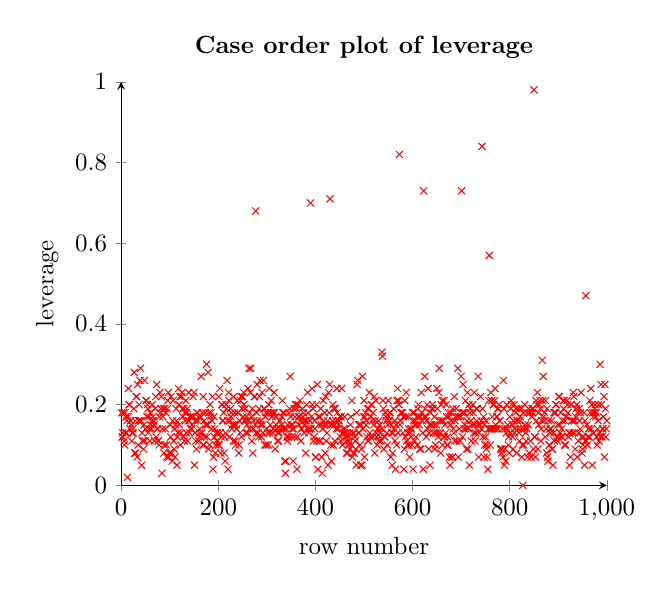
\begin{tikzpicture}[scale=0.9]
	\begin{axis}[
	xmin=0, xmax=1000, xlabel=row number,
	ymin=0, ymax=1, ylabel=leverage,
	axis x line=bottom,
	axis y line=left,
	title=\textbf{Case order plot of leverage}
	]
	\addplot[mark=x,red, only marks] coordinates {
		(1.00,0.18)
		(2.00,0.12)
		(3.00,0.13)
		(4.00,0.12)
		(5.00,0.18)
		(6.00,0.11)
		(7.00,0.10)
		(8.00,0.18)
		(9.00,0.13)
		(10.00,0.17)
		(11.00,0.13)
		(12.00,0.16)
		(13.00,0.02)
		(14.00,0.17)
		(15.00,0.24)
		(16.00,0.20)
		(17.00,0.20)
		(18.00,0.14)
		(19.00,0.16)
		(20.00,0.16)
		(21.00,0.15)
		(22.00,0.11)
		(23.00,0.13)
		(24.00,0.14)
		(25.00,0.13)
		(26.00,0.19)
		(27.00,0.28)
		(28.00,0.08)
		(29.00,0.16)
		(30.00,0.08)
		(31.00,0.22)
		(32.00,0.22)
		(33.00,0.07)
		(34.00,0.25)
		(35.00,0.10)
		(36.00,0.16)
		(37.00,0.20)
		(38.00,0.16)
		(39.00,0.26)
		(40.00,0.29)
		(41.00,0.16)
		(42.00,0.05)
		(43.00,0.13)
		(44.00,0.11)
		(45.00,0.11)
		(46.00,0.09)
		(47.00,0.15)
		(48.00,0.26)
		(49.00,0.11)
		(50.00,0.14)
		(51.00,0.21)
		(52.00,0.21)
		(53.00,0.17)
		(54.00,0.20)
		(55.00,0.19)
		(56.00,0.13)
		(57.00,0.17)
		(58.00,0.14)
		(59.00,0.11)
		(60.00,0.18)
		(61.00,0.15)
		(62.00,0.14)
		(63.00,0.16)
		(64.00,0.20)
		(65.00,0.17)
		(66.00,0.16)
		(67.00,0.16)
		(68.00,0.15)
		(69.00,0.11)
		(70.00,0.19)
		(71.00,0.22)
		(72.00,0.12)
		(73.00,0.25)
		(74.00,0.14)
		(75.00,0.14)
		(76.00,0.11)
		(77.00,0.11)
		(78.00,0.10)
		(79.00,0.17)
		(80.00,0.23)
		(81.00,0.18)
		(82.00,0.19)
		(83.00,0.22)
		(84.00,0.03)
		(85.00,0.14)
		(86.00,0.17)
		(87.00,0.19)
		(88.00,0.08)
		(89.00,0.10)
		(90.00,0.19)
		(91.00,0.14)
		(92.00,0.18)
		(93.00,0.10)
		(94.00,0.07)
		(95.00,0.19)
		(96.00,0.21)
		(97.00,0.23)
		(98.00,0.07)
		(99.00,0.08)
		(100.00,0.08)
		(101.00,0.15)
		(102.00,0.12)
		(103.00,0.22)
		(104.00,0.08)
		(105.00,0.06)
		(106.00,0.16)
		(107.00,0.21)
		(108.00,0.11)
		(109.00,0.09)
		(110.00,0.14)
		(111.00,0.07)
		(112.00,0.15)
		(113.00,0.19)
		(114.00,0.16)
		(115.00,0.05)
		(116.00,0.12)
		(117.00,0.13)
		(118.00,0.24)
		(119.00,0.20)
		(120.00,0.15)
		(121.00,0.22)
		(122.00,0.10)
		(123.00,0.13)
		(124.00,0.22)
		(125.00,0.23)
		(126.00,0.19)
		(127.00,0.17)
		(128.00,0.12)
		(129.00,0.19)
		(130.00,0.11)
		(131.00,0.18)
		(132.00,0.16)
		(133.00,0.21)
		(134.00,0.13)
		(135.00,0.18)
		(136.00,0.19)
		(137.00,0.11)
		(138.00,0.16)
		(139.00,0.23)
		(140.00,0.16)
		(141.00,0.13)
		(142.00,0.17)
		(143.00,0.14)
		(144.00,0.17)
		(145.00,0.14)
		(146.00,0.15)
		(147.00,0.17)
		(148.00,0.22)
		(149.00,0.17)
		(150.00,0.23)
		(151.00,0.05)
		(152.00,0.13)
		(153.00,0.16)
		(154.00,0.11)
		(155.00,0.09)
		(156.00,0.18)
		(157.00,0.18)
		(158.00,0.16)
		(159.00,0.17)
		(160.00,0.11)
		(161.00,0.13)
		(162.00,0.14)
		(163.00,0.12)
		(164.00,0.17)
		(165.00,0.27)
		(166.00,0.13)
		(167.00,0.18)
		(168.00,0.10)
		(169.00,0.22)
		(170.00,0.10)
		(171.00,0.16)
		(172.00,0.12)
		(173.00,0.18)
		(174.00,0.15)
		(175.00,0.15)
		(176.00,0.30)
		(177.00,0.12)
		(178.00,0.15)
		(179.00,0.28)
		(180.00,0.09)
		(181.00,0.18)
		(182.00,0.10)
		(183.00,0.20)
		(184.00,0.17)
		(185.00,0.18)
		(186.00,0.14)
		(187.00,0.16)
		(188.00,0.22)
		(189.00,0.04)
		(190.00,0.07)
		(191.00,0.17)
		(192.00,0.12)
		(193.00,0.14)
		(194.00,0.08)
		(195.00,0.10)
		(196.00,0.13)
		(197.00,0.11)
		(198.00,0.11)
		(199.00,0.13)
		(200.00,0.10)
		(201.00,0.22)
		(202.00,0.10)
		(203.00,0.24)
		(204.00,0.13)
		(205.00,0.08)
		(206.00,0.12)
		(207.00,0.20)
		(208.00,0.20)
		(209.00,0.16)
		(210.00,0.16)
		(211.00,0.18)
		(212.00,0.08)
		(213.00,0.12)
		(214.00,0.06)
		(215.00,0.13)
		(216.00,0.20)
		(217.00,0.19)
		(218.00,0.26)
		(219.00,0.16)
		(220.00,0.04)
		(221.00,0.23)
		(222.00,0.21)
		(223.00,0.12)
		(224.00,0.16)
		(225.00,0.19)
		(226.00,0.17)
		(227.00,0.18)
		(228.00,0.14)
		(229.00,0.15)
		(230.00,0.15)
		(231.00,0.11)
		(232.00,0.22)
		(233.00,0.15)
		(234.00,0.18)
		(235.00,0.11)
		(236.00,0.10)
		(237.00,0.15)
		(238.00,0.14)
		(239.00,0.21)
		(240.00,0.18)
		(241.00,0.18)
		(242.00,0.08)
		(243.00,0.10)
		(244.00,0.16)
		(245.00,0.13)
		(246.00,0.21)
		(247.00,0.22)
		(248.00,0.12)
		(249.00,0.19)
		(250.00,0.22)
		(251.00,0.17)
		(252.00,0.23)
		(253.00,0.20)
		(254.00,0.16)
		(255.00,0.19)
		(256.00,0.16)
		(257.00,0.13)
		(258.00,0.17)
		(259.00,0.15)
		(260.00,0.13)
		(261.00,0.24)
		(262.00,0.16)
		(263.00,0.29)
		(264.00,0.14)
		(265.00,0.18)
		(266.00,0.23)
		(267.00,0.29)
		(268.00,0.17)
		(269.00,0.11)
		(270.00,0.19)
		(271.00,0.08)
		(272.00,0.14)
		(273.00,0.16)
		(274.00,0.22)
		(275.00,0.22)
		(276.00,0.15)
		(277.00,0.68)
		(278.00,0.13)
		(279.00,0.18)
		(280.00,0.25)
		(281.00,0.16)
		(282.00,0.13)
		(283.00,0.12)
		(284.00,0.19)
		(285.00,0.22)
		(286.00,0.26)
		(287.00,0.15)
		(288.00,0.16)
		(289.00,0.12)
		(290.00,0.23)
		(291.00,0.15)
		(292.00,0.13)
		(293.00,0.26)
		(294.00,0.19)
		(295.00,0.19)
		(296.00,0.10)
		(297.00,0.17)
		(298.00,0.18)
		(299.00,0.10)
		(300.00,0.14)
		(301.00,0.13)
		(302.00,0.18)
		(303.00,0.10)
		(304.00,0.20)
		(305.00,0.24)
		(306.00,0.13)
		(307.00,0.15)
		(308.00,0.18)
		(309.00,0.21)
		(310.00,0.18)
		(311.00,0.17)
		(312.00,0.13)
		(313.00,0.14)
		(314.00,0.18)
		(315.00,0.23)
		(316.00,0.18)
		(317.00,0.09)
		(318.00,0.17)
		(319.00,0.15)
		(320.00,0.14)
		(321.00,0.14)
		(322.00,0.11)
		(323.00,0.13)
		(324.00,0.11)
		(325.00,0.13)
		(326.00,0.16)
		(327.00,0.16)
		(328.00,0.14)
		(329.00,0.14)
		(330.00,0.15)
		(331.00,0.17)
		(332.00,0.21)
		(333.00,0.18)
		(334.00,0.14)
		(335.00,0.18)
		(336.00,0.14)
		(337.00,0.06)
		(338.00,0.03)
		(339.00,0.06)
		(340.00,0.14)
		(341.00,0.12)
		(342.00,0.11)
		(343.00,0.15)
		(344.00,0.12)
		(345.00,0.12)
		(346.00,0.18)
		(347.00,0.19)
		(348.00,0.27)
		(349.00,0.17)
		(350.00,0.15)
		(351.00,0.12)
		(352.00,0.14)
		(353.00,0.15)
		(354.00,0.06)
		(355.00,0.14)
		(356.00,0.19)
		(357.00,0.12)
		(358.00,0.17)
		(359.00,0.20)
		(360.00,0.20)
		(361.00,0.19)
		(362.00,0.04)
		(363.00,0.12)
		(364.00,0.20)
		(365.00,0.17)
		(366.00,0.15)
		(367.00,0.17)
		(368.00,0.21)
		(369.00,0.16)
		(370.00,0.11)
		(371.00,0.14)
		(372.00,0.14)
		(373.00,0.19)
		(374.00,0.17)
		(375.00,0.18)
		(376.00,0.16)
		(377.00,0.13)
		(378.00,0.15)
		(379.00,0.16)
		(380.00,0.08)
		(381.00,0.16)
		(382.00,0.20)
		(383.00,0.14)
		(384.00,0.23)
		(385.00,0.18)
		(386.00,0.13)
		(387.00,0.14)
		(388.00,0.14)
		(389.00,0.16)
		(390.00,0.70)
		(391.00,0.14)
		(392.00,0.17)
		(393.00,0.24)
		(394.00,0.20)
		(395.00,0.19)
		(396.00,0.11)
		(397.00,0.12)
		(398.00,0.16)
		(399.00,0.14)
		(400.00,0.07)
		(401.00,0.07)
		(402.00,0.20)
		(403.00,0.11)
		(404.00,0.25)
		(405.00,0.04)
		(406.00,0.17)
		(407.00,0.15)
		(408.00,0.11)
		(409.00,0.17)
		(410.00,0.11)
		(411.00,0.19)
		(412.00,0.15)
		(413.00,0.07)
		(414.00,0.03)
		(415.00,0.14)
		(416.00,0.21)
		(417.00,0.16)
		(418.00,0.15)
		(419.00,0.18)
		(420.00,0.08)
		(421.00,0.22)
		(422.00,0.11)
		(423.00,0.15)
		(424.00,0.13)
		(425.00,0.16)
		(426.00,0.05)
		(427.00,0.23)
		(428.00,0.18)
		(429.00,0.25)
		(430.00,0.71)
		(431.00,0.15)
		(432.00,0.10)
		(433.00,0.06)
		(434.00,0.15)
		(435.00,0.16)
		(436.00,0.20)
		(437.00,0.10)
		(438.00,0.19)
		(439.00,0.15)
		(440.00,0.11)
		(441.00,0.19)
		(442.00,0.16)
		(443.00,0.14)
		(444.00,0.24)
		(445.00,0.18)
		(446.00,0.14)
		(447.00,0.16)
		(448.00,0.15)
		(449.00,0.16)
		(450.00,0.17)
		(451.00,0.12)
		(452.00,0.11)
		(453.00,0.17)
		(454.00,0.24)
		(455.00,0.13)
		(456.00,0.10)
		(457.00,0.14)
		(458.00,0.13)
		(459.00,0.13)
		(460.00,0.17)
		(461.00,0.14)
		(462.00,0.12)
		(463.00,0.13)
		(464.00,0.08)
		(465.00,0.11)
		(466.00,0.08)
		(467.00,0.12)
		(468.00,0.10)
		(469.00,0.11)
		(470.00,0.13)
		(471.00,0.09)
		(472.00,0.15)
		(473.00,0.17)
		(474.00,0.10)
		(475.00,0.21)
		(476.00,0.07)
		(477.00,0.13)
		(478.00,0.08)
		(479.00,0.13)
		(480.00,0.08)
		(481.00,0.12)
		(482.00,0.11)
		(483.00,0.09)
		(484.00,0.05)
		(485.00,0.18)
		(486.00,0.25)
		(487.00,0.26)
		(488.00,0.13)
		(489.00,0.15)
		(490.00,0.13)
		(491.00,0.15)
		(492.00,0.10)
		(493.00,0.05)
		(494.00,0.15)
		(495.00,0.09)
		(496.00,0.05)
		(497.00,0.27)
		(498.00,0.14)
		(499.00,0.17)
		(500.00,0.21)
		(501.00,0.07)
		(502.00,0.17)
		(503.00,0.18)
		(504.00,0.15)
		(505.00,0.16)
		(506.00,0.12)
		(507.00,0.19)
		(508.00,0.11)
		(509.00,0.11)
		(510.00,0.19)
		(511.00,0.23)
		(512.00,0.13)
		(513.00,0.12)
		(514.00,0.17)
		(515.00,0.20)
		(516.00,0.20)
		(517.00,0.16)
		(518.00,0.12)
		(519.00,0.18)
		(520.00,0.15)
		(521.00,0.22)
		(522.00,0.08)
		(523.00,0.16)
		(524.00,0.21)
		(525.00,0.13)
		(526.00,0.12)
		(527.00,0.10)
		(528.00,0.14)
		(529.00,0.14)
		(530.00,0.16)
		(531.00,0.11)
		(532.00,0.15)
		(533.00,0.12)
		(534.00,0.13)
		(535.00,0.11)
		(536.00,0.14)
		(537.00,0.33)
		(538.00,0.32)
		(539.00,0.21)
		(540.00,0.19)
		(541.00,0.09)
		(542.00,0.12)
		(543.00,0.12)
		(544.00,0.18)
		(545.00,0.17)
		(546.00,0.16)
		(547.00,0.13)
		(548.00,0.10)
		(549.00,0.15)
		(550.00,0.21)
		(551.00,0.17)
		(552.00,0.16)
		(553.00,0.18)
		(554.00,0.18)
		(555.00,0.07)
		(556.00,0.15)
		(557.00,0.13)
		(558.00,0.05)
		(559.00,0.08)
		(560.00,0.13)
		(561.00,0.19)
		(562.00,0.14)
		(563.00,0.16)
		(564.00,0.11)
		(565.00,0.04)
		(566.00,0.15)
		(567.00,0.10)
		(568.00,0.21)
		(569.00,0.24)
		(570.00,0.13)
		(571.00,0.21)
		(572.00,0.20)
		(573.00,0.82)
		(574.00,0.15)
		(575.00,0.16)
		(576.00,0.18)
		(577.00,0.18)
		(578.00,0.18)
		(579.00,0.18)
		(580.00,0.13)
		(581.00,0.17)
		(582.00,0.04)
		(583.00,0.09)
		(584.00,0.21)
		(585.00,0.12)
		(586.00,0.17)
		(587.00,0.23)
		(588.00,0.11)
		(589.00,0.10)
		(590.00,0.13)
		(591.00,0.17)
		(592.00,0.14)
		(593.00,0.10)
		(594.00,0.07)
		(595.00,0.13)
		(596.00,0.14)
		(597.00,0.12)
		(598.00,0.14)
		(599.00,0.10)
		(600.00,0.18)
		(601.00,0.04)
		(602.00,0.16)
		(603.00,0.18)
		(604.00,0.11)
		(605.00,0.15)
		(606.00,0.16)
		(607.00,0.12)
		(608.00,0.15)
		(609.00,0.17)
		(610.00,0.10)
		(611.00,0.19)
		(612.00,0.20)
		(613.00,0.17)
		(614.00,0.15)
		(615.00,0.09)
		(616.00,0.17)
		(617.00,0.09)
		(618.00,0.23)
		(619.00,0.18)
		(620.00,0.16)
		(621.00,0.13)
		(622.00,0.04)
		(623.00,0.73)
		(624.00,0.17)
		(625.00,0.27)
		(626.00,0.19)
		(627.00,0.17)
		(628.00,0.12)
		(629.00,0.16)
		(630.00,0.20)
		(631.00,0.14)
		(632.00,0.24)
		(633.00,0.09)
		(634.00,0.13)
		(635.00,0.15)
		(636.00,0.05)
		(637.00,0.18)
		(638.00,0.15)
		(639.00,0.15)
		(640.00,0.19)
		(641.00,0.20)
		(642.00,0.19)
		(643.00,0.13)
		(644.00,0.15)
		(645.00,0.17)
		(646.00,0.09)
		(647.00,0.10)
		(648.00,0.13)
		(649.00,0.15)
		(650.00,0.24)
		(651.00,0.19)
		(652.00,0.13)
		(653.00,0.12)
		(654.00,0.23)
		(655.00,0.29)
		(656.00,0.16)
		(657.00,0.13)
		(658.00,0.08)
		(659.00,0.20)
		(660.00,0.16)
		(661.00,0.21)
		(662.00,0.10)
		(663.00,0.16)
		(664.00,0.12)
		(665.00,0.21)
		(666.00,0.12)
		(667.00,0.15)
		(668.00,0.13)
		(669.00,0.20)
		(670.00,0.17)
		(671.00,0.10)
		(672.00,0.12)
		(673.00,0.10)
		(674.00,0.18)
		(675.00,0.17)
		(676.00,0.07)
		(677.00,0.05)
		(678.00,0.15)
		(679.00,0.18)
		(680.00,0.16)
		(681.00,0.07)
		(682.00,0.07)
		(683.00,0.19)
		(684.00,0.14)
		(685.00,0.13)
		(686.00,0.22)
		(687.00,0.11)
		(688.00,0.16)
		(689.00,0.17)
		(690.00,0.19)
		(691.00,0.11)
		(692.00,0.17)
		(693.00,0.29)
		(694.00,0.07)
		(695.00,0.17)
		(696.00,0.14)
		(697.00,0.11)
		(698.00,0.11)
		(699.00,0.17)
		(700.00,0.27)
		(701.00,0.73)
		(702.00,0.18)
		(703.00,0.12)
		(704.00,0.25)
		(705.00,0.18)
		(706.00,0.14)
		(707.00,0.18)
		(708.00,0.15)
		(709.00,0.21)
		(710.00,0.14)
		(711.00,0.09)
		(712.00,0.16)
		(713.00,0.23)
		(714.00,0.09)
		(715.00,0.14)
		(716.00,0.20)
		(717.00,0.05)
		(718.00,0.18)
		(719.00,0.19)
		(720.00,0.16)
		(721.00,0.11)
		(722.00,0.15)
		(723.00,0.15)
		(724.00,0.20)
		(725.00,0.18)
		(726.00,0.13)
		(727.00,0.23)
		(728.00,0.15)
		(729.00,0.11)
		(730.00,0.13)
		(731.00,0.19)
		(732.00,0.16)
		(733.00,0.19)
		(734.00,0.15)
		(735.00,0.27)
		(736.00,0.07)
		(737.00,0.13)
		(738.00,0.15)
		(739.00,0.15)
		(740.00,0.22)
		(741.00,0.16)
		(742.00,0.14)
		(743.00,0.84)
		(744.00,0.19)
		(745.00,0.12)
		(746.00,0.17)
		(747.00,0.07)
		(748.00,0.15)
		(749.00,0.10)
		(750.00,0.12)
		(751.00,0.16)
		(752.00,0.09)
		(753.00,0.10)
		(754.00,0.07)
		(755.00,0.04)
		(756.00,0.14)
		(757.00,0.21)
		(758.00,0.57)
		(759.00,0.14)
		(760.00,0.10)
		(761.00,0.23)
		(762.00,0.14)
		(763.00,0.21)
		(764.00,0.17)
		(765.00,0.14)
		(766.00,0.20)
		(767.00,0.20)
		(768.00,0.14)
		(769.00,0.21)
		(770.00,0.24)
		(771.00,0.15)
		(772.00,0.14)
		(773.00,0.17)
		(774.00,0.17)
		(775.00,0.19)
		(776.00,0.14)
		(777.00,0.19)
		(778.00,0.20)
		(779.00,0.16)
		(780.00,0.16)
		(781.00,0.09)
		(782.00,0.09)
		(783.00,0.08)
		(784.00,0.09)
		(785.00,0.14)
		(786.00,0.07)
		(787.00,0.26)
		(788.00,0.19)
		(789.00,0.05)
		(790.00,0.09)
		(791.00,0.14)
		(792.00,0.06)
		(793.00,0.13)
		(794.00,0.20)
		(795.00,0.14)
		(796.00,0.15)
		(797.00,0.10)
		(798.00,0.12)
		(799.00,0.08)
		(800.00,0.17)
		(801.00,0.13)
		(802.00,0.19)
		(803.00,0.21)
		(804.00,0.20)
		(805.00,0.15)
		(806.00,0.12)
		(807.00,0.09)
		(808.00,0.16)
		(809.00,0.20)
		(810.00,0.13)
		(811.00,0.14)
		(812.00,0.18)
		(813.00,0.19)
		(814.00,0.08)
		(815.00,0.16)
		(816.00,0.16)
		(817.00,0.14)
		(818.00,0.19)
		(819.00,0.13)
		(820.00,0.11)
		(821.00,0.16)
		(822.00,0.17)
		(823.00,0.14)
		(824.00,0.19)
		(825.00,0.07)
		(826.00,0.10)
		(827.00,-0.00)
		(828.00,0.18)
		(829.00,0.10)
		(830.00,0.14)
		(831.00,0.20)
		(832.00,0.15)
		(833.00,0.13)
		(834.00,0.11)
		(835.00,0.14)
		(836.00,0.18)
		(837.00,0.07)
		(838.00,0.15)
		(839.00,0.19)
		(840.00,0.08)
		(841.00,0.18)
		(842.00,0.18)
		(843.00,0.11)
		(844.00,0.07)
		(845.00,0.17)
		(846.00,0.19)
		(847.00,0.18)
		(848.00,0.19)
		(849.00,0.09)
		(850.00,0.98)
		(851.00,0.12)
		(852.00,0.12)
		(853.00,0.07)
		(854.00,0.21)
		(855.00,0.16)
		(856.00,0.20)
		(857.00,0.23)
		(858.00,0.09)
		(859.00,0.18)
		(860.00,0.15)
		(861.00,0.20)
		(862.00,0.21)
		(863.00,0.19)
		(864.00,0.11)
		(865.00,0.14)
		(866.00,0.16)
		(867.00,0.31)
		(868.00,0.21)
		(869.00,0.27)
		(870.00,0.17)
		(871.00,0.16)
		(872.00,0.18)
		(873.00,0.12)
		(874.00,0.21)
		(875.00,0.14)
		(876.00,0.08)
		(877.00,0.19)
		(878.00,0.07)
		(879.00,0.06)
		(880.00,0.16)
		(881.00,0.10)
		(882.00,0.10)
		(883.00,0.14)
		(884.00,0.13)
		(885.00,0.14)
		(886.00,0.16)
		(887.00,0.09)
		(888.00,0.09)
		(889.00,0.05)
		(890.00,0.13)
		(891.00,0.18)
		(892.00,0.11)
		(893.00,0.18)
		(894.00,0.18)
		(895.00,0.20)
		(896.00,0.20)
		(897.00,0.12)
		(898.00,0.11)
		(899.00,0.15)
		(900.00,0.12)
		(901.00,0.22)
		(902.00,0.22)
		(903.00,0.15)
		(904.00,0.13)
		(905.00,0.18)
		(906.00,0.12)
		(907.00,0.14)
		(908.00,0.12)
		(909.00,0.16)
		(910.00,0.21)
		(911.00,0.19)
		(912.00,0.21)
		(913.00,0.10)
		(914.00,0.16)
		(915.00,0.10)
		(916.00,0.17)
		(917.00,0.17)
		(918.00,0.21)
		(919.00,0.20)
		(920.00,0.18)
		(921.00,0.12)
		(922.00,0.13)
		(923.00,0.05)
		(924.00,0.13)
		(925.00,0.07)
		(926.00,0.20)
		(927.00,0.20)
		(928.00,0.16)
		(929.00,0.13)
		(930.00,0.16)
		(931.00,0.23)
		(932.00,0.22)
		(933.00,0.13)
		(934.00,0.16)
		(935.00,0.09)
		(936.00,0.17)
		(937.00,0.19)
		(938.00,0.20)
		(939.00,0.07)
		(940.00,0.18)
		(941.00,0.11)
		(942.00,0.13)
		(943.00,0.19)
		(944.00,0.16)
		(945.00,0.14)
		(946.00,0.18)
		(947.00,0.23)
		(948.00,0.12)
		(949.00,0.08)
		(950.00,0.09)
		(951.00,0.10)
		(952.00,0.12)
		(953.00,0.18)
		(954.00,0.05)
		(955.00,0.16)
		(956.00,0.11)
		(957.00,0.47)
		(958.00,0.11)
		(959.00,0.15)
		(960.00,0.10)
		(961.00,0.12)
		(962.00,0.14)
		(963.00,0.14)
		(964.00,0.12)
		(965.00,0.21)
		(966.00,0.18)
		(967.00,0.24)
		(968.00,0.14)
		(969.00,0.20)
		(970.00,0.05)
		(971.00,0.18)
		(972.00,0.17)
		(973.00,0.13)
		(974.00,0.18)
		(975.00,0.19)
		(976.00,0.20)
		(977.00,0.17)
		(978.00,0.18)
		(979.00,0.12)
		(980.00,0.10)
		(981.00,0.14)
		(982.00,0.16)
		(983.00,0.20)
		(984.00,0.11)
		(985.00,0.13)
		(986.00,0.30)
		(987.00,0.12)
		(988.00,0.25)
		(989.00,0.20)
		(990.00,0.12)
		(991.00,0.14)
		(992.00,0.14)
		(993.00,0.17)
		(994.00,0.22)
		(995.00,0.07)
		(996.00,0.25)
		(997.00,0.19)
		(998.00,0.12)
		(999.00,0.14)
		(1000.00,0.16)
	};
	\end{axis}
	\end{tikzpicture}
\end{center}

Measures like Leverage and \person{Cook}'s distance can be used to look for outliers in the data.

\textbf{Warning:} MATLAB uses raw residuals as default.

\subsection{Hypothesis tests on GLM fits}

As for LMs, hypothesis tests for individual parameters have been developed. They test the hypothesis that $Y$ does not change as an explanatory changes. In other words, we test hypotheses like: \\
$H_0$: $\beta_1=0$ \\
$H_A$: $\beta_1\neq 0$ \\
... we skip the details of these tests (different software may using different tests).

As discussed previously, we could also use Likelihood-ratio tests to look at similar hypotheses. For global tests on the entire model, the Likelihood-ratio test can be used. E.g. for a model with $p$ parameters, compare the fitted model to the constant model by testing: \\
$H_0$: $\beta_1=\dots=\beta_{p-1}=0$

\subsection{Model selection on GLMs}

Model selection for GLMs proceeds in a similar way to what we discussed for LMs. However, some tests that were developed specifically for LMs are not usually appropriate.

AIC and BIC can always be used.

To compare nested models, the Likelihood-ratio test can be  used (versions of the F-test can only be used with great caution). Parameter-specific tests are available (although the likelihood-ratio test could be used for this). A similar measure to $R^2$ exists (\begriff{Deviance}). It is based on comparing the likelihood of the model to a \begriff{saturated model} with one parameter per data point.

\subsection{Interpreting GLM parameters}

From our model formulation and fit, we find that
\begin{align}
	\mu_i = \frac{1}{1+\exp(-(-13.38+0.0042\cdot weight_i))} \notag
\end{align}

\begin{center}
	\begin{tikzpicture}
	\begin{axis}[
	xmin=2000, xmax=4500, xlabel=weight (kg),
	ymin=0, ymax=1, ylabel=proportion of cars that fail,
	title=\textbf{cars failing mileage tests},
	axis x line=bottom,
	axis y line=left,
	domain=2000:4500,
	]
	\addplot[blue, only marks, mark=x] coordinates {
		(2100.00,0.02)
		(2300.00,0.05)
		(2500.00,0.00)
		(2700.00,0.09)
		(2900.00,0.26)
		(3100.00,0.38)
		(3300.00,0.61)
		(3500.00,0.74)
		(3700.00,0.90)
		(3900.00,0.94)
		(4100.00,1.00)
		(4300.00,1.00)
	};
	\addplot[cyan] {1/(1+exp(-(-13.38 + 0.0042*x)))};
	\end{axis}
	\end{tikzpicture}
\end{center}

Unlike for linear models, we cannot read off effect sizes directly from parameter estimates in GLMs. \textcolor{red}{Need to consider the link function.}

\pagebreak

\section{Appendix}
\subsection{\person{Weibulls} Distribution - Graphs}

\begin{center}
    \begin{tabular}{p{5cm}|p{5cm}|p{5cm}}
        $shape = 0.5$ & $shape = 1$ & $shape = 2$ \\
        \hline
        \multicolumn{3}{c}{\cellcolor{gray!50}\textbf{Weibull PDF} ($scale = 1$)} \\
        \hline
        \begin{tikzpicture}[scale=0.6]
            \begin{axis}[
		    xmin=0, xmax=2, xlabel=$x$,
		    ymin=0, ymax=1, ylabel=$y$,
		    samples=400,
		    axis y line=middle,
		    axis x line=middle,
		    ]
		    \addplot+[mark=none] {0.5*x^(-0.5)*exp(-x^0.5)};
		    \end{axis}
        \end{tikzpicture} &
        \begin{tikzpicture}[scale=0.6]
            \begin{axis}[
		    xmin=0, xmax=2, xlabel=$x$,
		    ymin=0, ymax=1, ylabel=$y$,
		    samples=400,
		    axis y line=middle,
		    axis x line=middle,
		    restrict y to domain=0:1,
		    ]
		    \addplot+[mark=none] {1/exp(x)};
		    \end{axis}
        \end{tikzpicture} &
        \begin{tikzpicture}[scale=0.6]
            \begin{axis}[
		    xmin=0, xmax=2, xlabel=$x$,
		    ymin=0, ymax=1, ylabel=$y$,
		    samples=400,
		    axis y line=middle,
		    axis x line=middle,
		    ]
		    \addplot+[mark=none] {2*x^(1)*exp(-x^2)};
		    \end{axis}
        \end{tikzpicture} \\
        \hline
        \multicolumn{3}{c}{\cellcolor{gray!50}\textbf{Weibull CDF} ($scale = 1$)} \\
        \hline
        \begin{tikzpicture}[scale=0.6]
            \begin{axis}[
		    xmin=0, xmax=2, xlabel=$x$,
		    ymin=0, ymax=1, ylabel=$y$,
		    samples=400,
		    axis y line=middle,
		    axis x line=middle,
		    ]
		    \addplot+[mark=none] {1-exp(-x^0.5)};
		    \end{axis}
        \end{tikzpicture} &
        \begin{tikzpicture}[scale=0.6]
            \begin{axis}[
		    xmin=0, xmax=2, xlabel=$x$,
		    ymin=0, ymax=1, ylabel=$y$,
		    samples=400,
		    axis y line=middle,
		    axis x line=middle,
		    restrict y to domain=0:1,
		    ]
		    \addplot+[mark=none] {1-1/exp(x)};
		    \end{axis}
        \end{tikzpicture} &
        \begin{tikzpicture}[scale=0.6]
            \begin{axis}[
		    xmin=0, xmax=2, xlabel=$x$,
		    ymin=0, ymax=1, ylabel=$y$,
		    samples=400,
		    axis y line=middle,
		    axis x line=middle,
		    ]
		    \addplot+[mark=none] {1-exp(-x^2)};
		    \end{axis}
        \end{tikzpicture} \\
        \hline
        \multicolumn{3}{c}{\cellcolor{gray!50}\textbf{Hazard function} $\left(h = \frac{\text{PDF}}{1-\text{CDF}}\right)$} \\
        \hline
        \begin{tikzpicture}[scale=0.6]
            \begin{axis}[
		    xmin=0, xmax=2, xlabel=$x$,
		    ymin=0, ymax=1, ylabel=$y$,
		    samples=400,
		    axis y line=middle,
		    axis x line=middle,
		    ]
		    \addplot+[mark=none] {(0.5*x^(-0.5)*exp(-x^0.5))/(1-(1-exp(-x^0.5)))};
		    \end{axis}
        \end{tikzpicture} &
        \begin{tikzpicture}[scale=0.6]
            \begin{axis}[
		    xmin=0, xmax=2, xlabel=$x$,
		    ymin=0, ymax=1, ylabel=$y$,
		    samples=400,
		    axis y line=middle,
		    axis x line=middle,
		    restrict y to domain=0:1,
		    ]
		    \addplot+[mark=none] {(1/exp(x))/(1-(1-1/exp(x)))};
		    \end{axis}
        \end{tikzpicture} &
        \begin{tikzpicture}[scale=0.6]
            \begin{axis}[
		    xmin=0, xmax=2, xlabel=$x$,
		    ymin=0, ymax=1, ylabel=$y$,
		    samples=400,
		    axis y line=middle,
		    axis x line=middle,
		    ]
		    \addplot+[mark=none] {(2*x^(1)*exp(-x^2))/(1-(1-exp(-x^2)))};
		    \end{axis}
        \end{tikzpicture} \\
        \hline
        \multicolumn{3}{c}{\cellcolor{gray!50}\textbf{Survival function} ($R = 1-\text{CDF}$)} \\
        \hline
        \begin{tikzpicture}[scale=0.6]
            \begin{axis}[
		    xmin=0, xmax=2, xlabel=$x$,
		    ymin=0, ymax=1, ylabel=$y$,
		    samples=400,
		    axis y line=middle,
		    axis x line=middle,
		    ]
		    \addplot+[mark=none] {1-(1-exp(-x^0.5))};
		    \end{axis}
        \end{tikzpicture} &
        \begin{tikzpicture}[scale=0.6]
            \begin{axis}[
		    xmin=0, xmax=2, xlabel=$x$,
		    ymin=0, ymax=1, ylabel=$y$,
		    samples=400,
		    axis y line=middle,
		    axis x line=middle,
		    restrict y to domain=0:1,
		    ]
		    \addplot+[mark=none] {1-(1-1/exp(x))};
		    \end{axis}
        \end{tikzpicture} &
        \begin{tikzpicture}[scale=0.6]
            \begin{axis}[
		    xmin=0, xmax=2, xlabel=$x$,
		    ymin=0, ymax=1, ylabel=$y$,
		    samples=400,
		    axis y line=middle,
		    axis x line=middle,
		    ]
		    \addplot+[mark=none] {1-(1-exp(-x^2))};
		    \end{axis}
        \end{tikzpicture} \\
    \end{tabular}
\end{center}
%\addcontentsline{toc}{part}{Appendix}
%\appendix

%\printglossary[type=\acronymtype]

\printindex

\end{document}
